\documentclass{templateReport}
\usepackage{tocloft} % Para personalizar el índice de contenidos
\usepackage{fontawesome5}
\hypersetup{
    colorlinks=true,        % Habilita el coloreado de enlaces
    linkcolor=black,         % Color de los enlaces internos (como la tabla de contenido)
    citecolor=blue,         % Color de las citas
    filecolor=blue,         % Color de los enlaces a archivos locales
    urlcolor=black           % Color de los enlaces URL
}
\usepackage{verbatim}
\tcbuselibrary{listingsutf8}
\usepackage{listings}
\definecolor{codebg}{rgb}{0.95, 0.95, 0.95}
\usepackage{graphicx}
\usepackage{tikz}
\lstset{
    language=SQL,
    basicstyle=\ttfamily\footnotesize,
    % backgroundcolor=\color{codebg},
    % frame=single,
    breaklines=true,
    keepspaces=true,
    showstringspaces=false,
    tabsize=4
}
\usepackage{caption}

% Algunos colores personalizados
\definecolor{Violeta}{RGB}{124,0,254}
\definecolor{Verde2}{RGB}{130,254,0} % Complementario
\definecolor{Naranja2}{RGB}{254,124,0} % Triadico
\definecolor{Verde3}{RGB}{0,254,124} % Triadico
\definecolor{Amarillo}{RGB}{249,228,0}
\definecolor{Azul2}{RGB}{0,21,249} % Complementario
\definecolor{Celeste2}{RGB}{0,249,228} % Triadico
\definecolor{Rosa}{RGB}{228,0,249} % Triadico
\definecolor{Naranja}{RGB}{255,175,0}
\definecolor{Azul3}{RGB}{0,80,255} % Complementario
\definecolor{Cian}{RGB}{0,255,175} % Triadico
\definecolor{Violeta2}{RGB}{175,0,255} % Triadico
\definecolor{Rojo}{RGB}{245,0,79}
\definecolor{Verde4}{RGB}{0,245,166} % Complementario
\definecolor{Verde}{RGB}{79,245,0} % Triadico
\definecolor{Azul}{RGB}{0,79,245} % Triadico
\definecolor{Celeste}{RGB}{0,191,255}
\definecolor{Salmon}{RGB}{255,0,157}

\newcommand{\newparagraph}{\par\vspace{\baselineskip}\noindent}
\newcommand{\hlcolor}[2]{{\sethlcolor{#1}\hl{#2}}}

% Personalizar el formato del índice de contenidos
\addto\captionsspanish{\renewcommand{\contentsname}{Índice de contenidos}} % Cambiar el título del índice de contenidos
\addto\captionsspanish{\renewcommand{\listtablename}{Índice de tablas}} % Cambiar el título del índice de tablas
\renewcommand{\cftsecleader}{\cftdotfill{\cftdotsep}} % Puntos entre el título y el número de página
\renewcommand{\cftsecfont}{} % Títulos de secciones en negrita
\renewcommand{\cftsecpagefont}{} % Números de página en negrita
\renewcommand{\cftsecindent}{1.5em}
\renewcommand{\cftsubsecindent}{2.5em}
\renewcommand{\cftsecnumwidth}{2.5em} 
\renewcommand{\cftsubsecnumwidth}{2.5em}

% Ajustar el espaciado antes y después de las secciones
\setlength{\cftbeforesecskip}{0.5em}
\setlength{\cftaftertoctitleskip}{1em}

% Cuadro personalizado
\tcbuselibrary{skins}
\usetikzlibrary{shadings}
\newcounter{contador}
\tcbset{
  base/.style={
    empty,
    frame engine=path,
    colframe=white,
    sharp corners,
    attach boxed title to top left={yshift*=-\tcboxedtitleheight},
    boxed title style={size=minimal, top=4pt, left=4pt},
    coltitle=black,
    fonttitle=\large\it,
  }
}
\newtcolorbox{CuadroPersonalizado}[5]{%
  base,
  title={#3 \csname the#2\endcsname}, % Título personalizado #2 = nombre contador ; #3 = Título
  drop fuzzy shadow, % Sombra del cuadro de texto
  coltitle=#1,
  borderline west={3pt}{-3pt}{#4}, % Borde Izquierdo #4 = color del borde
  attach boxed title to top left={xshift=-3mm, yshift*=-\tcboxedtitleheight/2},
  boxed title style={right=3pt, bottom=3pt, overlay={
    \draw[draw=#5, fill=#5, line join=round]
      (frame.south west) -- (frame.north west) -- (frame.north east) --
      (frame.south east) -- ++(-2pt, 0) -- ++(-2pt, -4pt) --
      ++(-2pt, 4pt) -- cycle; % #5 = color del fondo
  }}, % Cuadro de titulo
  overlay unbroken={
    \scoped \shade[left color=#5!30!black, right color=#5]
    ([yshift=-0.2pt]title.south west) -- ([xshift=-3pt, yshift=-0.2pt]title.south-|frame.west) -- ++(0, -4pt) -- cycle;
  }, % Sombra de titulo #5 = color del titulo
  before upper={\stepcounter{#2}}
}

\newtcolorbox{cPB}[2]{%
  base,
  coltitle=#1,
  borderline west={3pt}{-3pt}{#2}, % Borde izquierdo
  listing only, % Configura para mostrar solo código
  listing options={%
    basicstyle=\ttfamily,   % Fuente monoespaciada
    breaklines=true,        % Dividir líneas largas automáticamente
    keepspaces=true,        % Mantener espacios en blanco
    showstringspaces=false  % No mostrar espacios en cadenas
  },
  before skip=0pt,          % Quita espacio antes del cuadro
  after skip=0pt            % Quita espacio después del cuadro
}
\lstset{
  basicstyle=\ttfamily,  % Fuente monoespaciada
  % breaklines=true,       % Dividir líneas largas automáticamente
  keepspaces=true,       % Mantener espacios en blanco
  showstringspaces=false,
}
\newtcolorbox{warningbox}[1]{
	base,
	drop fuzzy shadow, % Sombra del cuadro de texto
	borderline west={3pt}{-3pt}{#1}, % Borde Izquierdo #4 = color del borde
  	coltitle=black, % Color del texto del título
  	left=18mm, % Espaciado izquierdo dentro del cuadro
  	overlay={%
    \node[anchor=west, xshift=3mm] at (frame.west) {%
      {\fontsize{24}{28}\selectfont\textcolor{#1}{\faExclamationTriangle}} % Tamaño ajustado del ícono
    };
  },
}

% Formato de la página
\fancypagestyle{plain}{
    \makenomenclature
    \pagestyle{fancy}
    \fancyheadoffset{1cm}
    \setlength{\headheight}{2cm}
    \lhead{\includegraphics[scale=0.3]{\imagenlogoDOS}}
    \rhead{\nouppercase{\leftmark}}
    \rfoot{\thepage}
    \cfoot{Informe - \textbf{\titulo}}
}

\begin{document}
\setcounter{contador}{1}

\imagenlogoUNO{img/UBBVertical.png} % El logo de la universidad tiene escrito "Universidad del Bío-Bío"
\imagenlogoDOS{img/UBBHorizontalNegro.png} % El logo para el encabezado del documento
\titulo{Proyecto: Asistencia digital} % Titulo del proyecto
\integrantes{
	\hspace*{2cm}Marcelo Paz \\
	\hspace*{2cm}Bastián Rodríguez \\
} % Integrantes
\supervisor{
	\hspace*{2cm}Luis Vera
} % Supervisor

% Ingresar Metadatos para nombre y autores del documento
\title{[CIMUBB-INFORME]-\titulo}
\author{
	\integrantes
	\supervisor
}

\portada % Crear portada
\margenes % Crear márgenes

\tableofcontents % Tabla de contenidos
\newpage
\listoffigures % Tabla de figuras
\listoftables % Tabla de tablas 

\newpage
\section{Introducción}

\subsection{Situación actual}
Respecto al estudio realizado en el establecimiento, se observó un gran flujo de personas que hacen ingreso al Laboratorio utilizando un registro de asistencia manual. Algunas de estas personas son trabajadores de la institución, estudiantes en prácticas o invitados. Existen ocasiones especiales, como exposiciones de maquetas o presentaciones de nuevas tecnologías en desarrollo, en la cual ingresa personal externo a la institución.

\subsection{Objetivos del proyecto}
\subsubsection{Objetivo general}
\begin{itemize}
	\item Construir un sistema de asistencia digital que permita conocer el ingreso y salida de los individuos dentro del laboratorio.
	\item Visualizar los datos registrados en un dashboard con información sobre el uso del espacio y las actividades principales.
\end{itemize}
\subsubsection{Objetivos específicos}
\begin{itemize}
	\item Recepción de datos de individuos.
	\item Validación de datos utilizando un API proporcionada por la Universidad del Bío-Bío.
	\item Almacenamiento de datos registrados.
	\item Visualización de datos registrados.
\end{itemize}

\newpage
\section{Análisis y Diseño}
\subsection{Diseño lógico}
\subsubsection{Modelo de entidad-relación}
\begin{figure}[H]
	\centering
	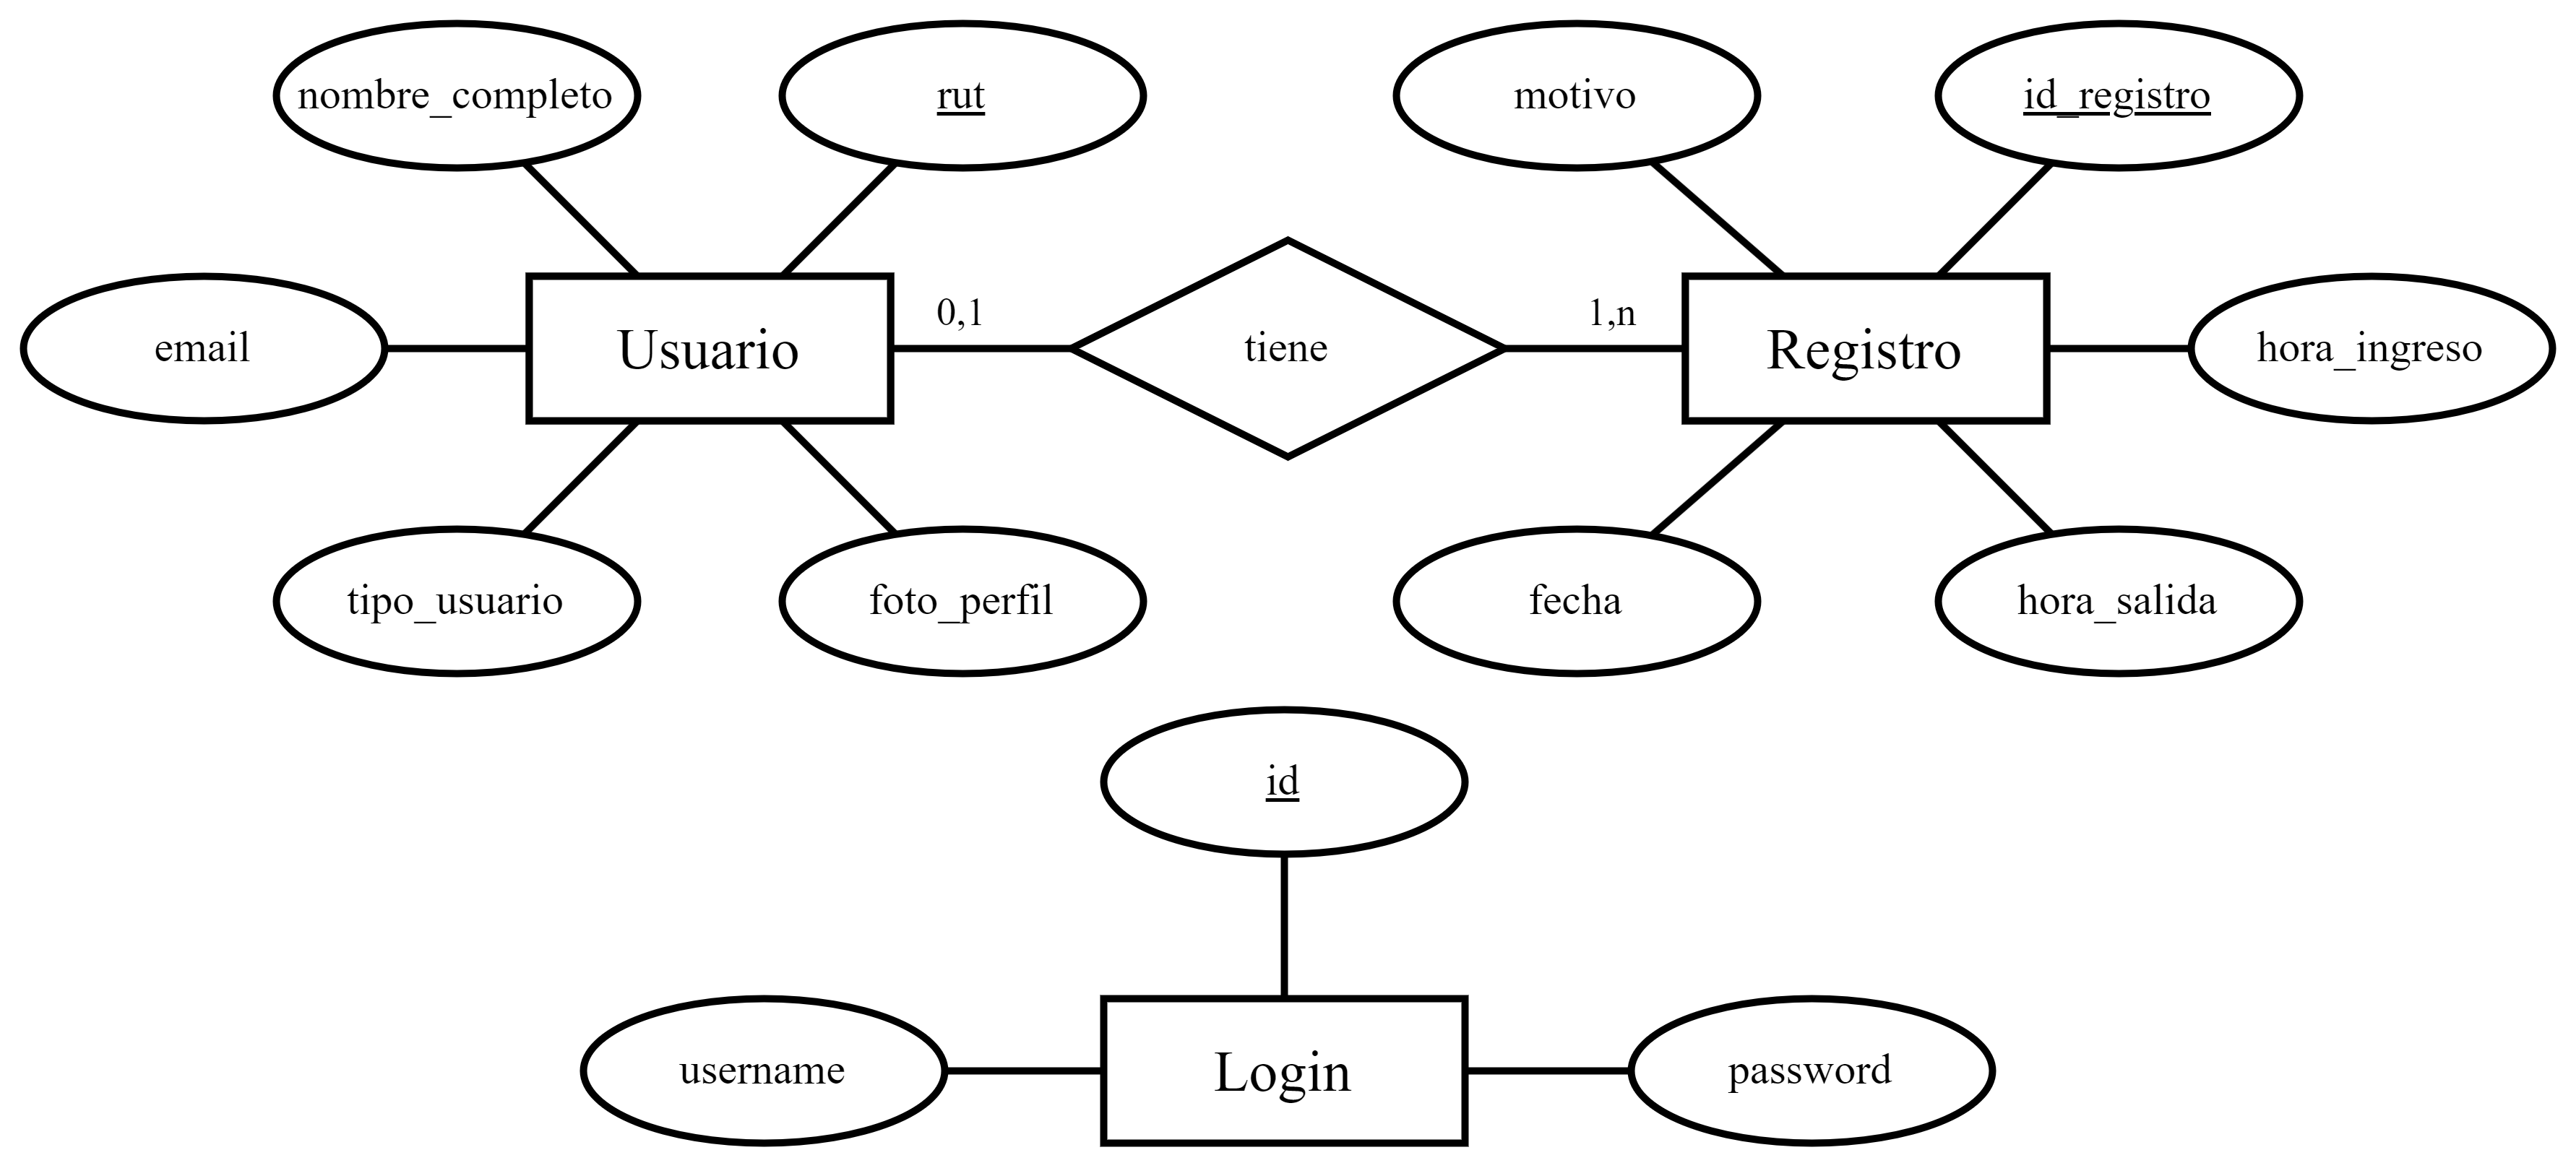
\includegraphics[scale=0.13]{img/TS-SI-MER.drawio.png}
	\caption{Modelo de entidad-relación}
	\label{fig:modeloEntidadRelacion}
\end{figure}


\subsubsection{Modelo relacional}
\begin{figure}[H]
	\centering
	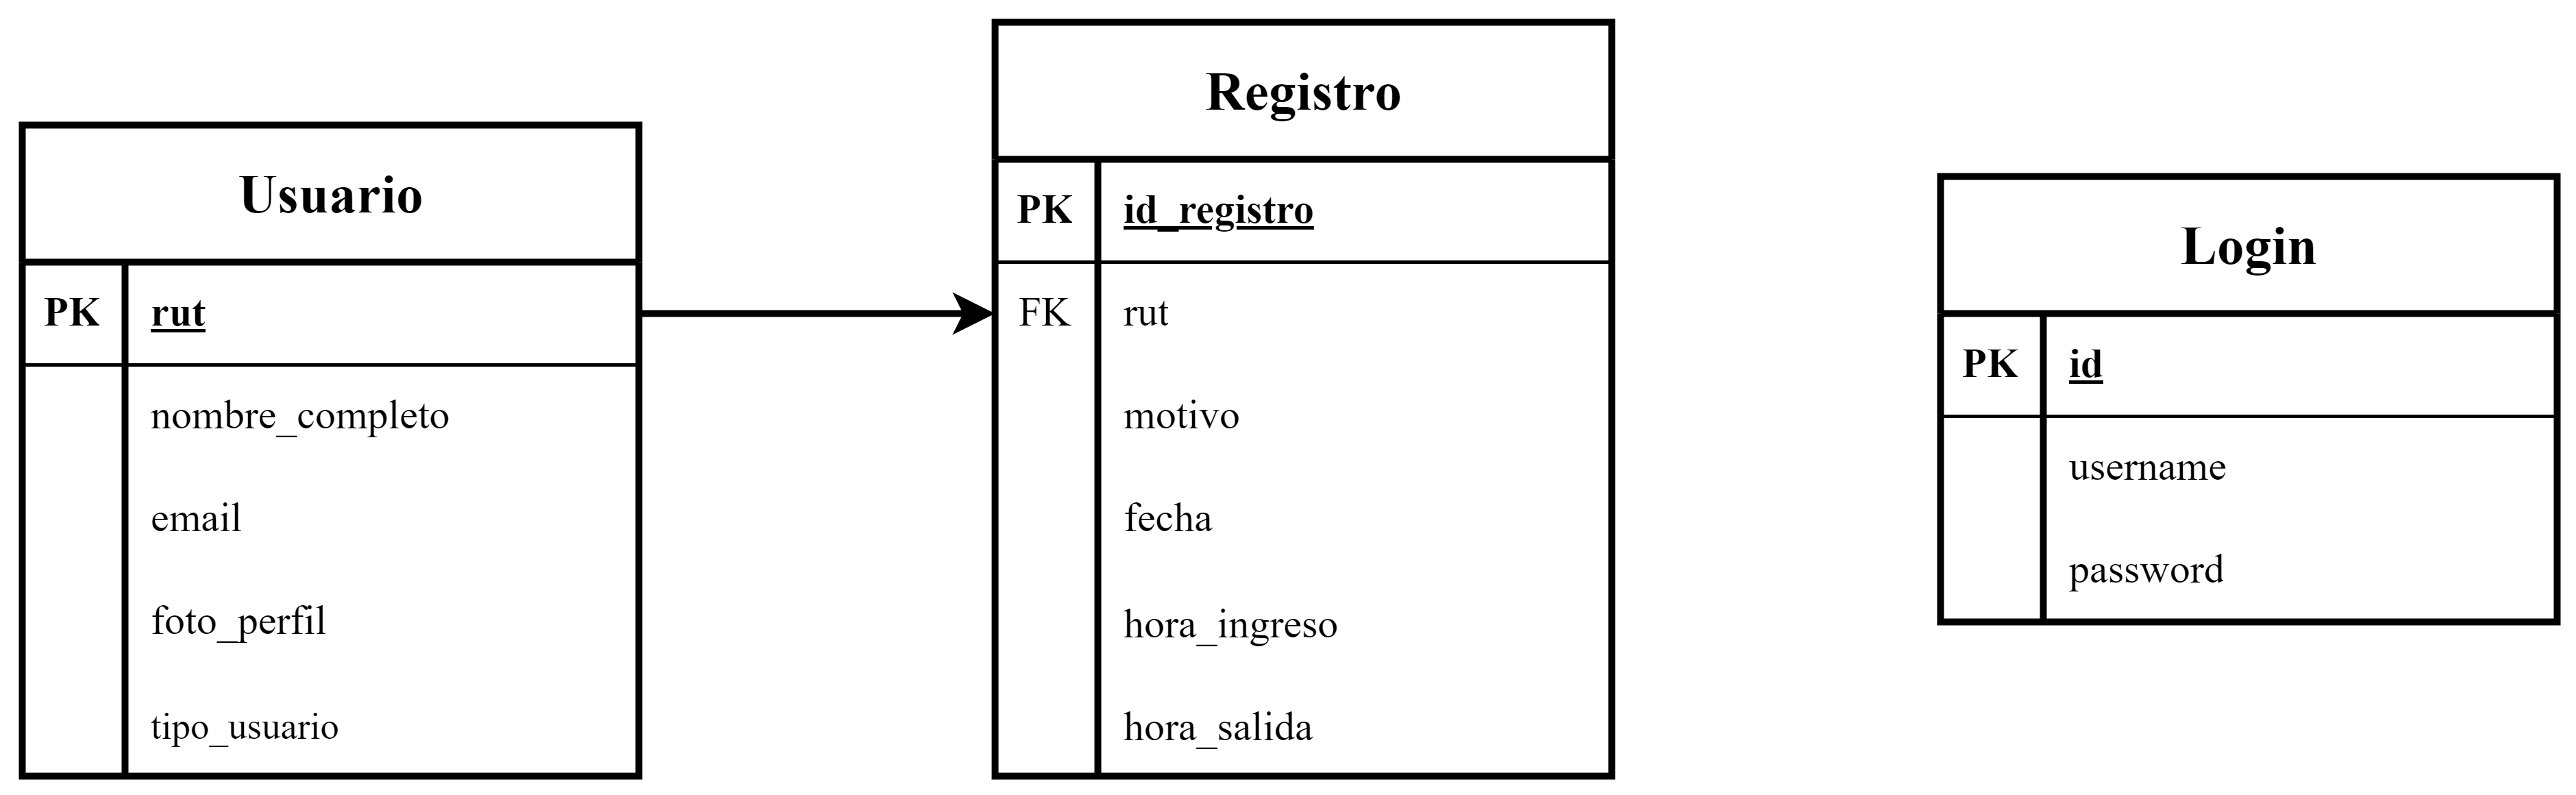
\includegraphics[scale=0.11]{img/TS-SI-MR.drawio.png}
	\caption{Modelo relacional}
	\label{fig:modeloRelacional}
\end{figure}

\subsubsection{Diagrama de contexto}
\begin{figure}[H]
	\centering
	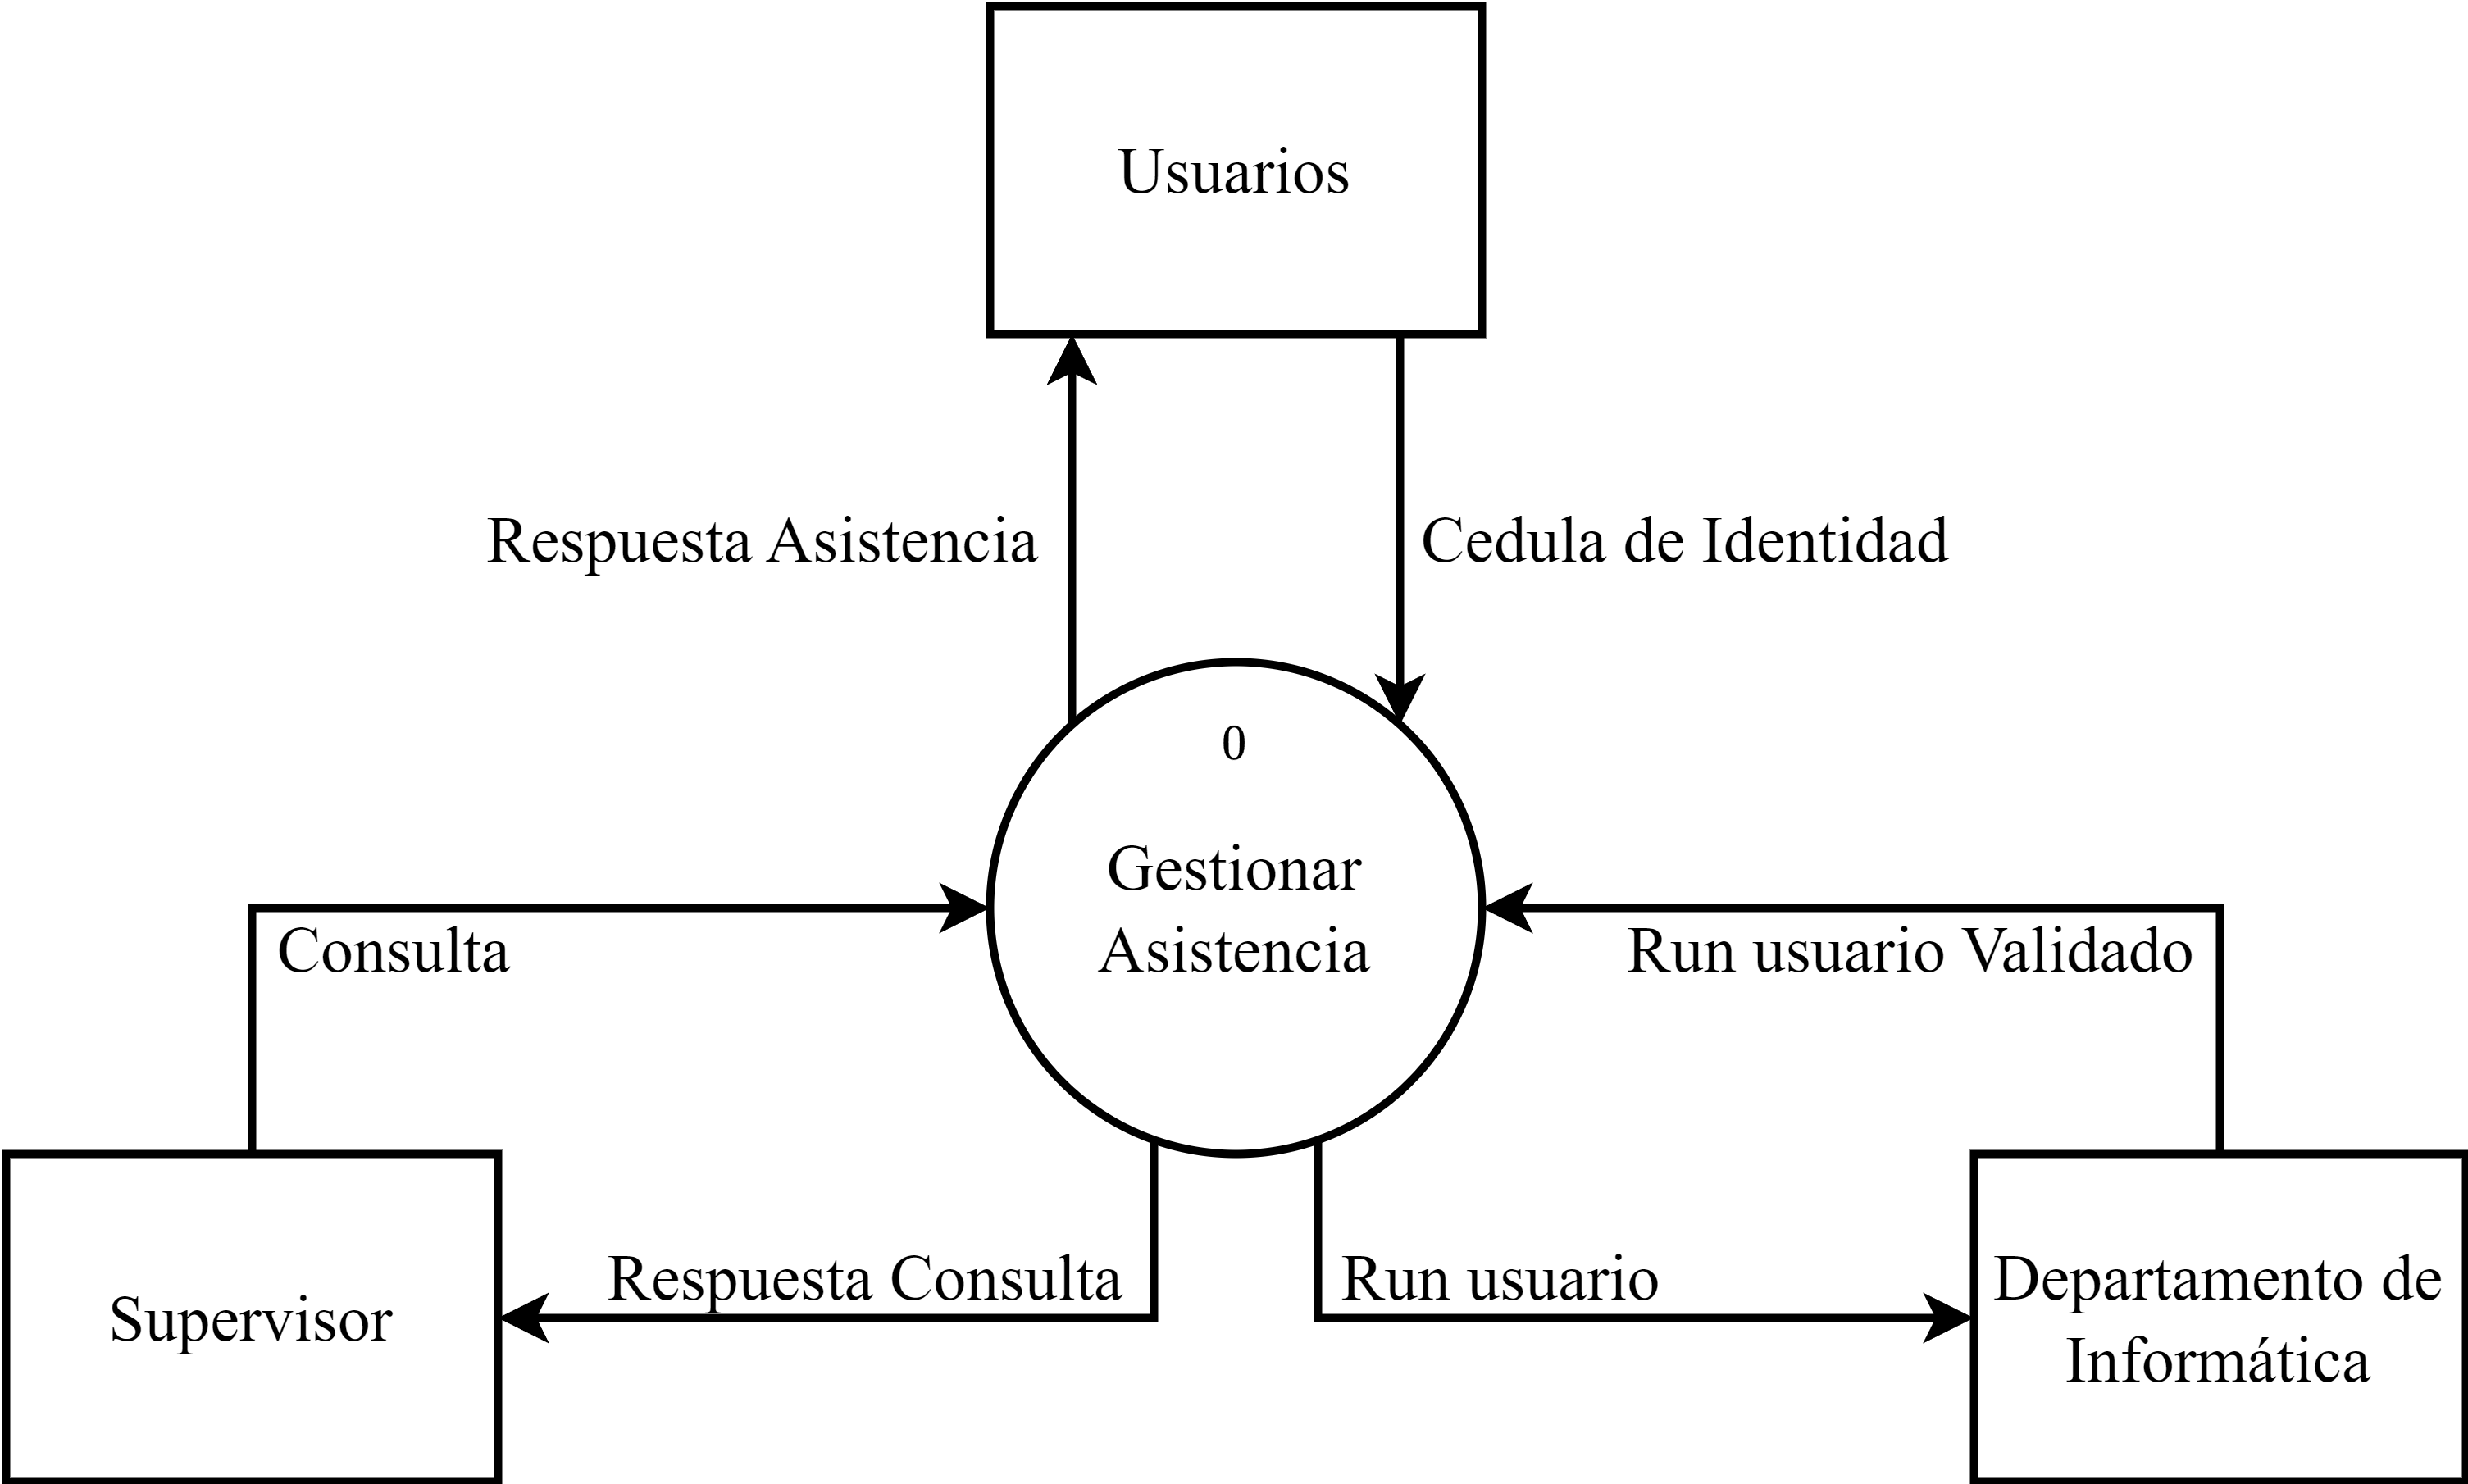
\includegraphics[scale=0.09]{img/TS-SI-Contexto.drawio.png}
	\caption{Diagrama de contexto}
	\label{fig:diagramaContexto}
\end{figure}
\subsubsection{Diagrama de nivel superior}
\begin{figure}[H]
	\centering
	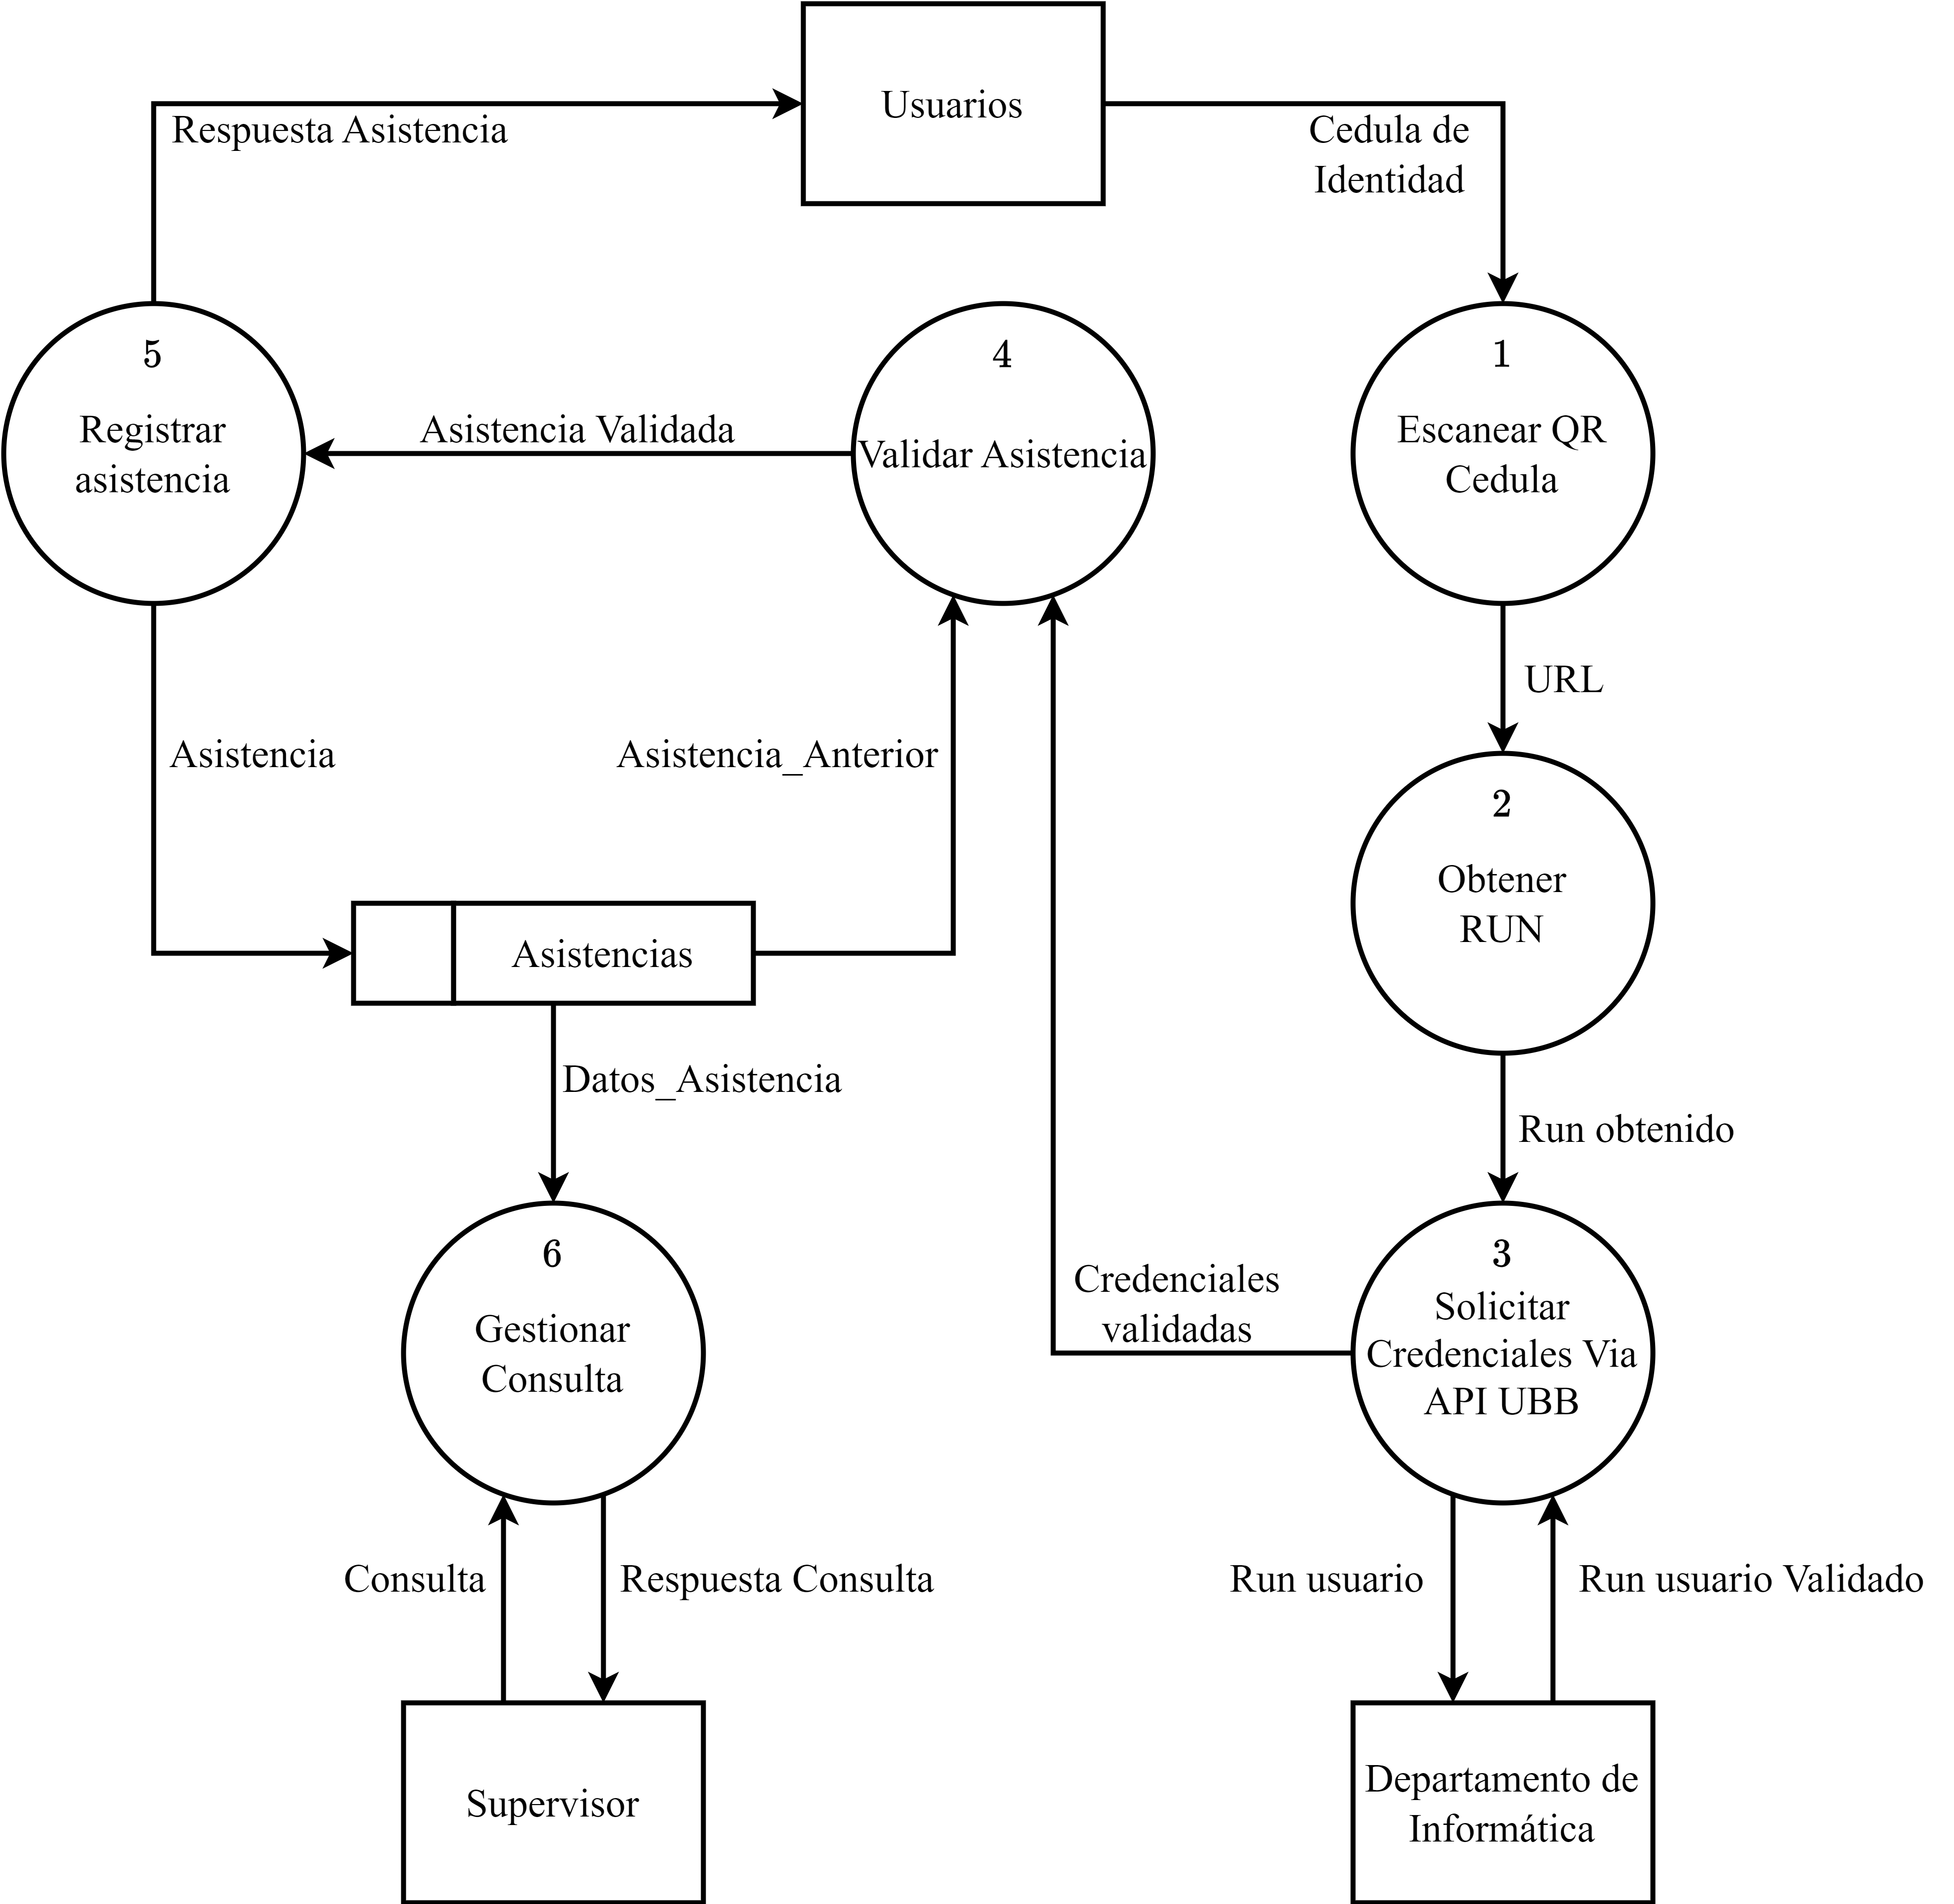
\includegraphics[scale=0.09]{img/TS-SI-Nivel Superior.drawio.png}
	\caption{Diagrama de nivel superior}
	\label{fig:diagramaNivelSuperior}
\end{figure}

\subsubsection{Procedimientos administrativos}
\begin{figure}[H]
	\centering
	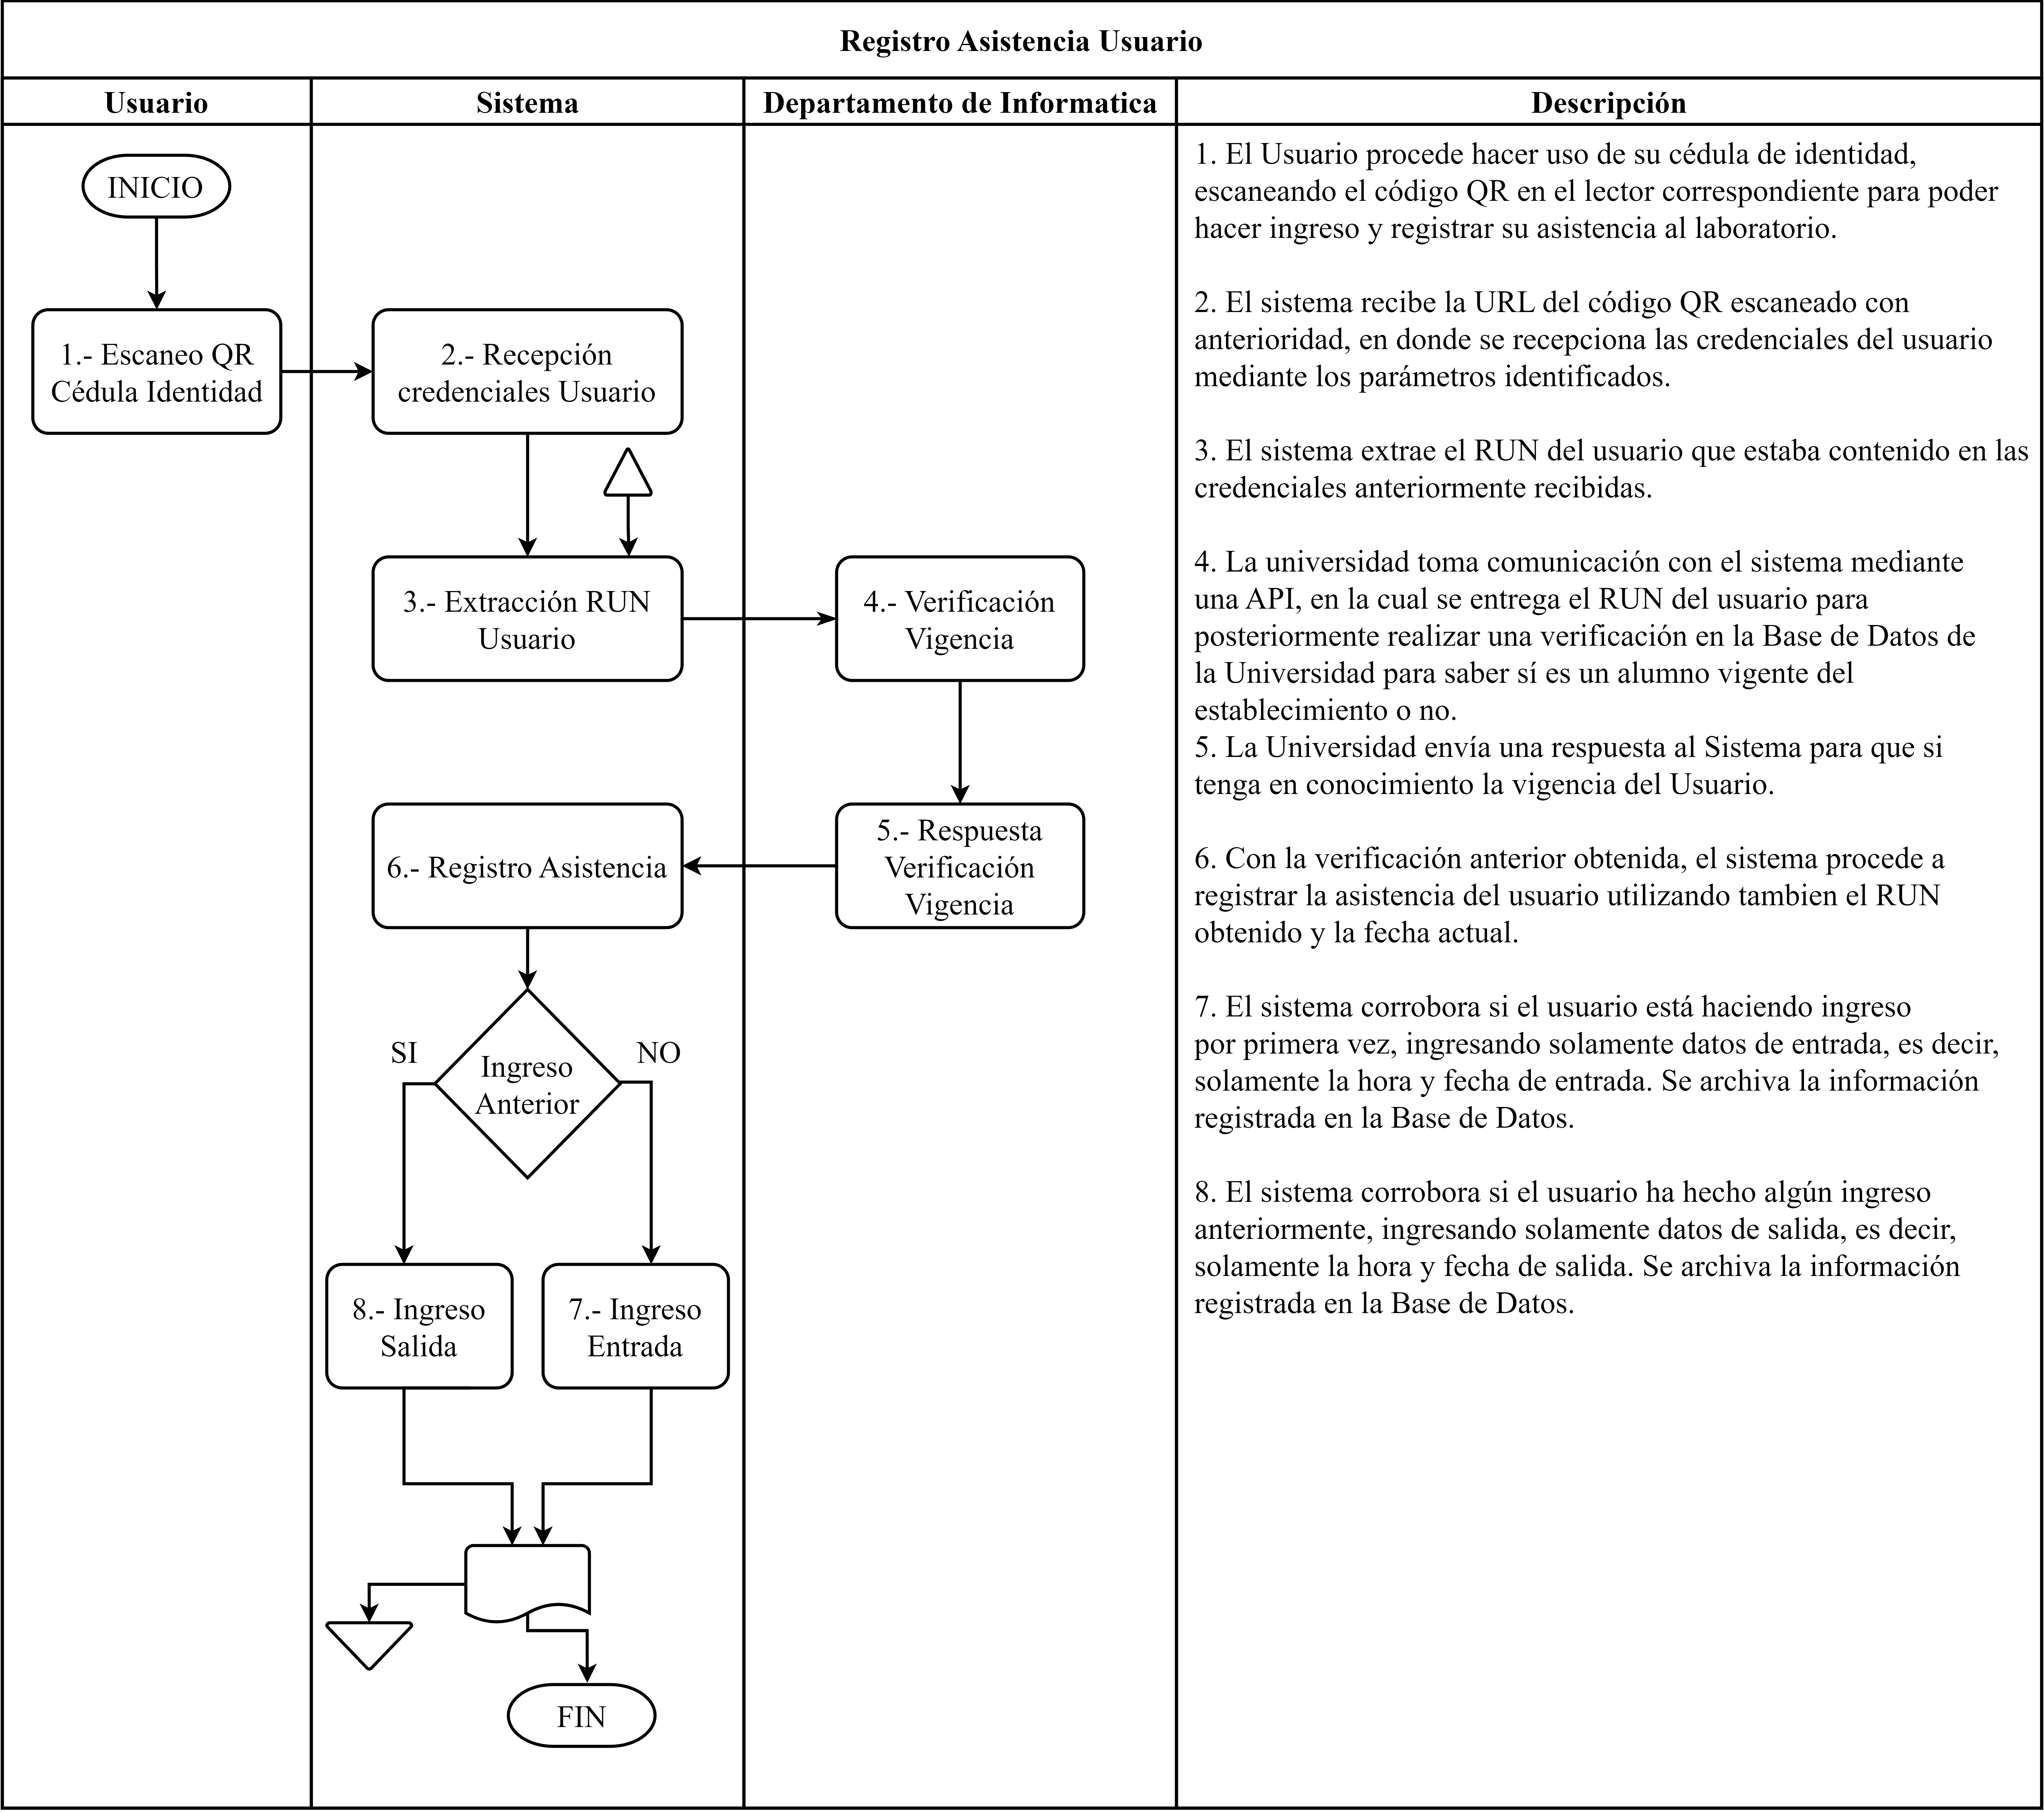
\includegraphics[scale=0.068]{img/TS-SI-Procedo Administrativo.drawio.png}
	\caption{Procedimientos administrativos}
	\label{fig:procedimientosAdministrativos}
\end{figure}

\newpage

\subsection{Diseño físico}
\subsubsection{Arquitectura del sistema}
\begin{figure}[H]
	\centering
	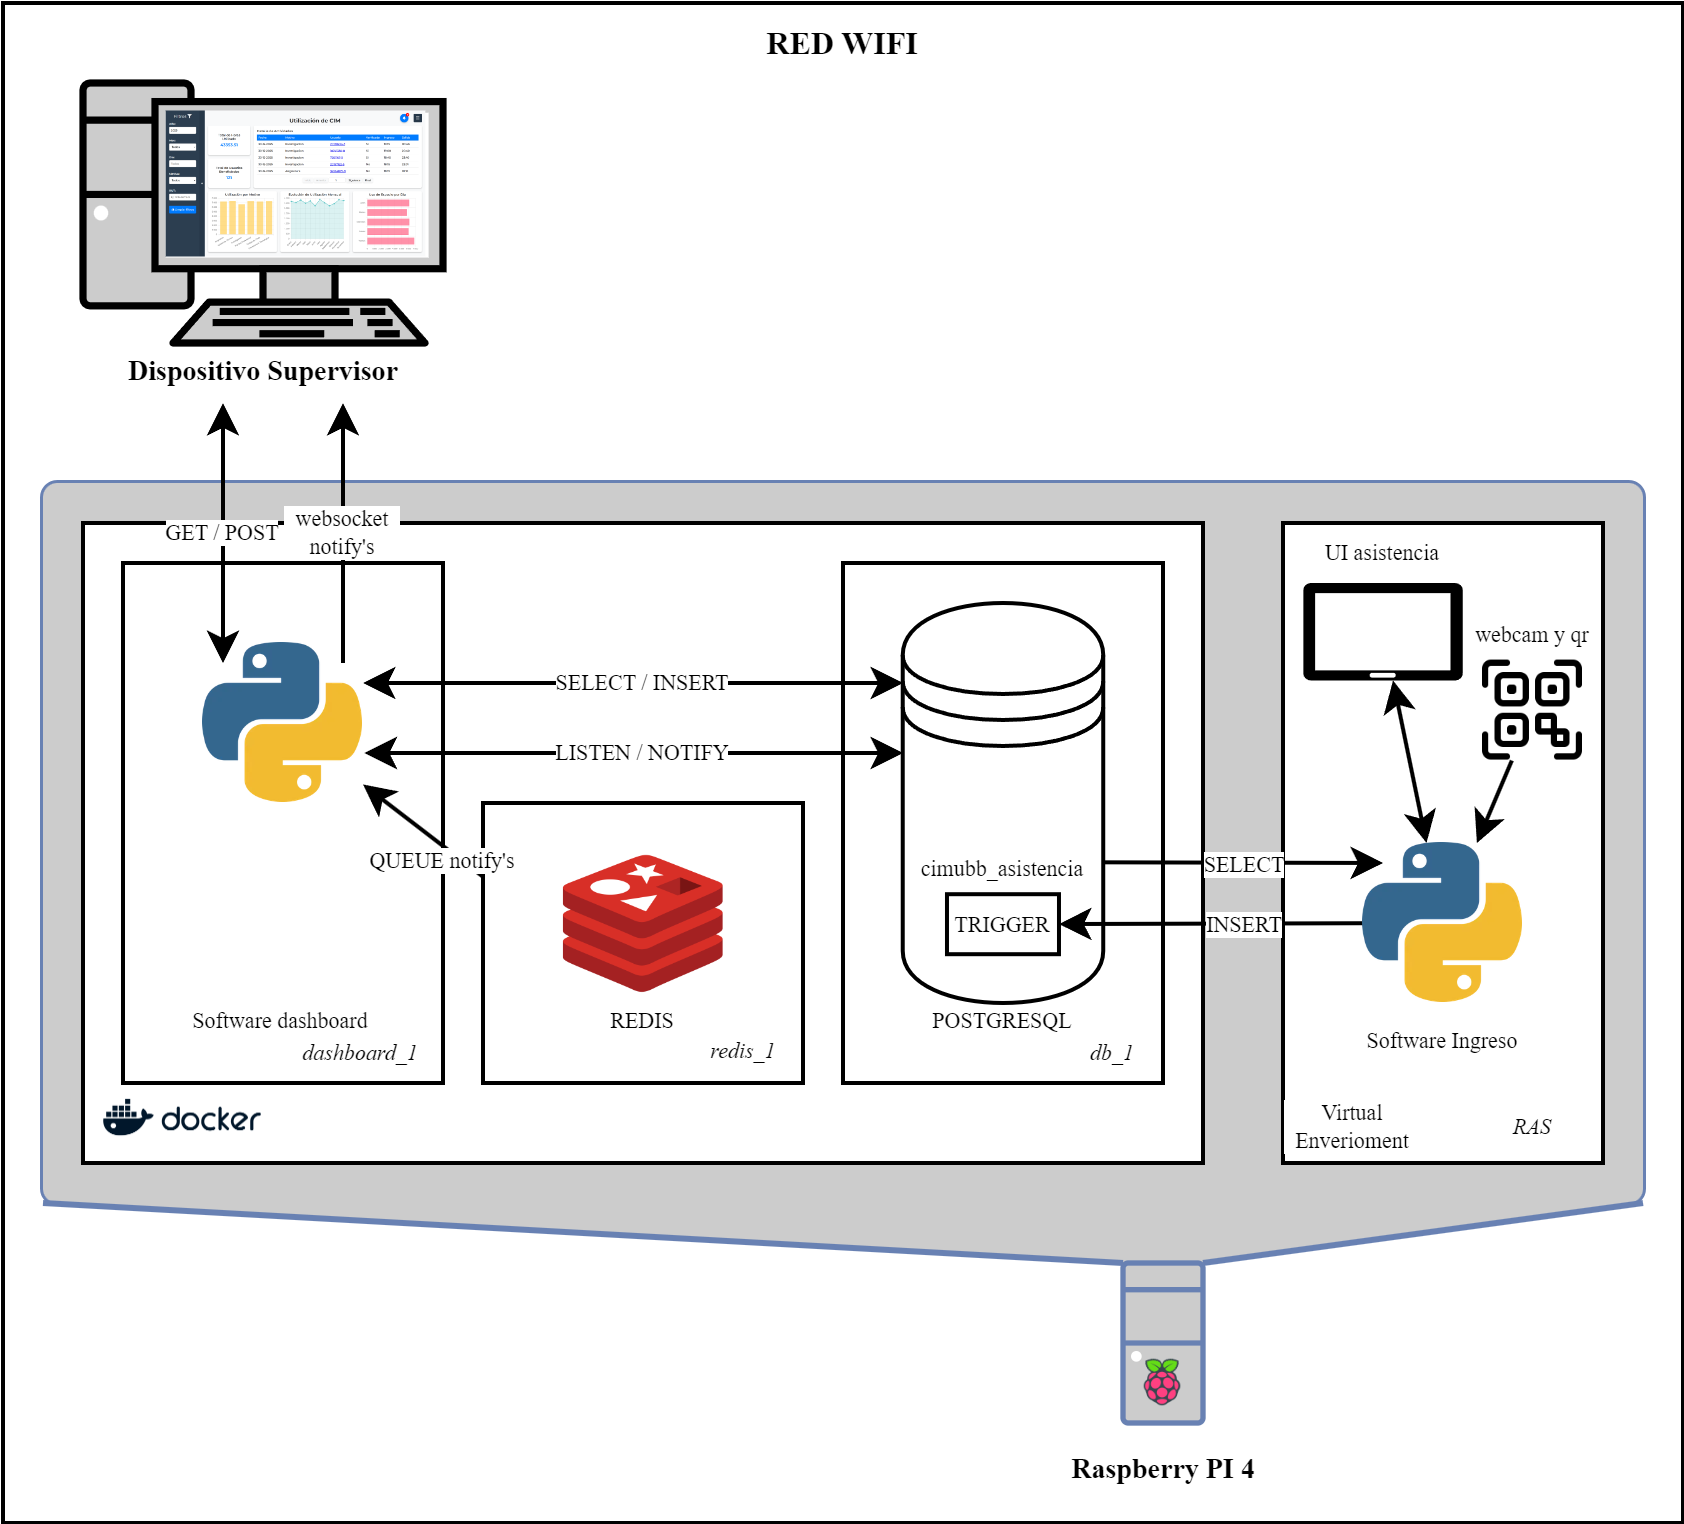
\includegraphics[scale=0.24]{img/TS-SI-Arquitectura.drawio.png}
	\caption{Arquitectura del sistema}
	\label{fig:arquitecturaSistema}
\end{figure}
Se decidió utilizar Docker para facilitar la implementación del software. En resumen, dentro de la raspberry tendremos 3 imagenes de Docker y un entorno virtual para el correcto funcionamiento de la aplicación de registro:
\begin{itemize}
	\item \textbf{dashboard\_1}: Se utiliza una imagen de python13 slim con la aplicación que controla el servicio web para la supervisión de los registros.
	\item \textbf{redis\_1}: Se utiliza una imagen oficial de redis para el guardado de notificaciones temporales, pues si no tenemos activo un WebSocket se pierden las notificaciones, por lo que el usar Redis de forma temporal nos resuelve este problema al utilizar una Queue.
	\item \textbf{db\_1}: Se utiliza una imagen oficial de postgres:17 para guardar nuestros datos y montar inicialmente la configuración.
	\item \textbf{RAS:} La aplicación encargada de mostrar una GUI para el registro de asistencias del laboratorio.
\end{itemize}

\newpage
\section{Documentación de Hardware}
\subsection{Raspberry Pi 4}
\begin{figure}[H]
	\centering
	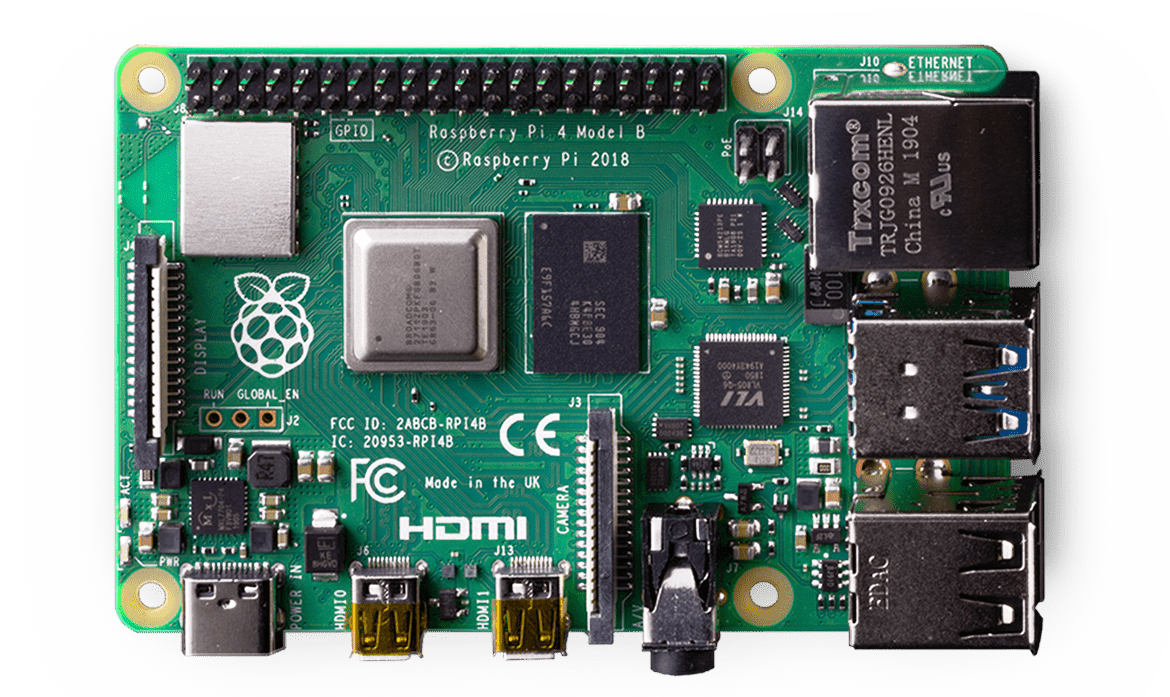
\includegraphics[scale=0.27]{img/Raspberry-Pi.png}
	\caption{Raspberry Pi 4 \cite{raspberryPi}}
	\label{fig:raspberryPi4}
\end{figure}
La Raspberry Pi 4 Model B de 8GB de RAM es utilizada en el proyecto por su capacidad para manejar aplicaciones intensivas en procesamiento y datos, su conectividad avanzada, que incluye Wi-Fi y Ethernet, asegura la comunicación eficiente con servidores o sistemas remotos, facilitando el monitoreo y notificación del ingreso de personal al laboratorio.
\subsection{Pantalla táctil de 7 pulgadas \textbf{[Se desconoce el modelo de pantalla]}}
\begin{figure}[H]
	\centering
	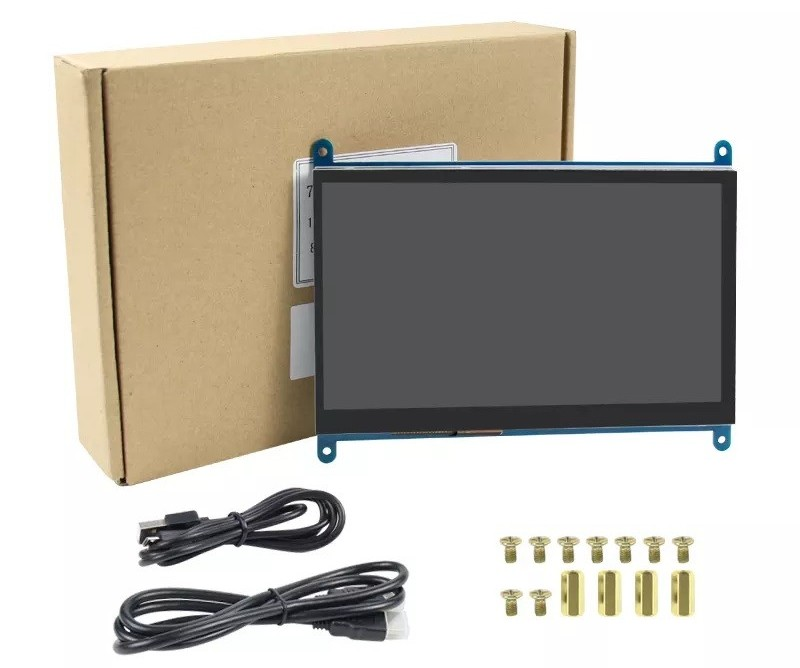
\includegraphics[scale=0.3]{img/PantallaTouch.jpg}
	\caption{Pantalla táctil de 7 pulgadas}
	\label{fig:pantallaTactil7Pulgadas}
\end{figure}
La pantalla táctil de 7 pulgadas es utilizada para mostrar el software de registro de asistencia, permitiendo a los usuarios ingresar su información personal y registrar su ingreso al laboratorio.

\newpage
\subsection{Logitech HD Webcam C270}
\begin{figure}[H]
	\centering
	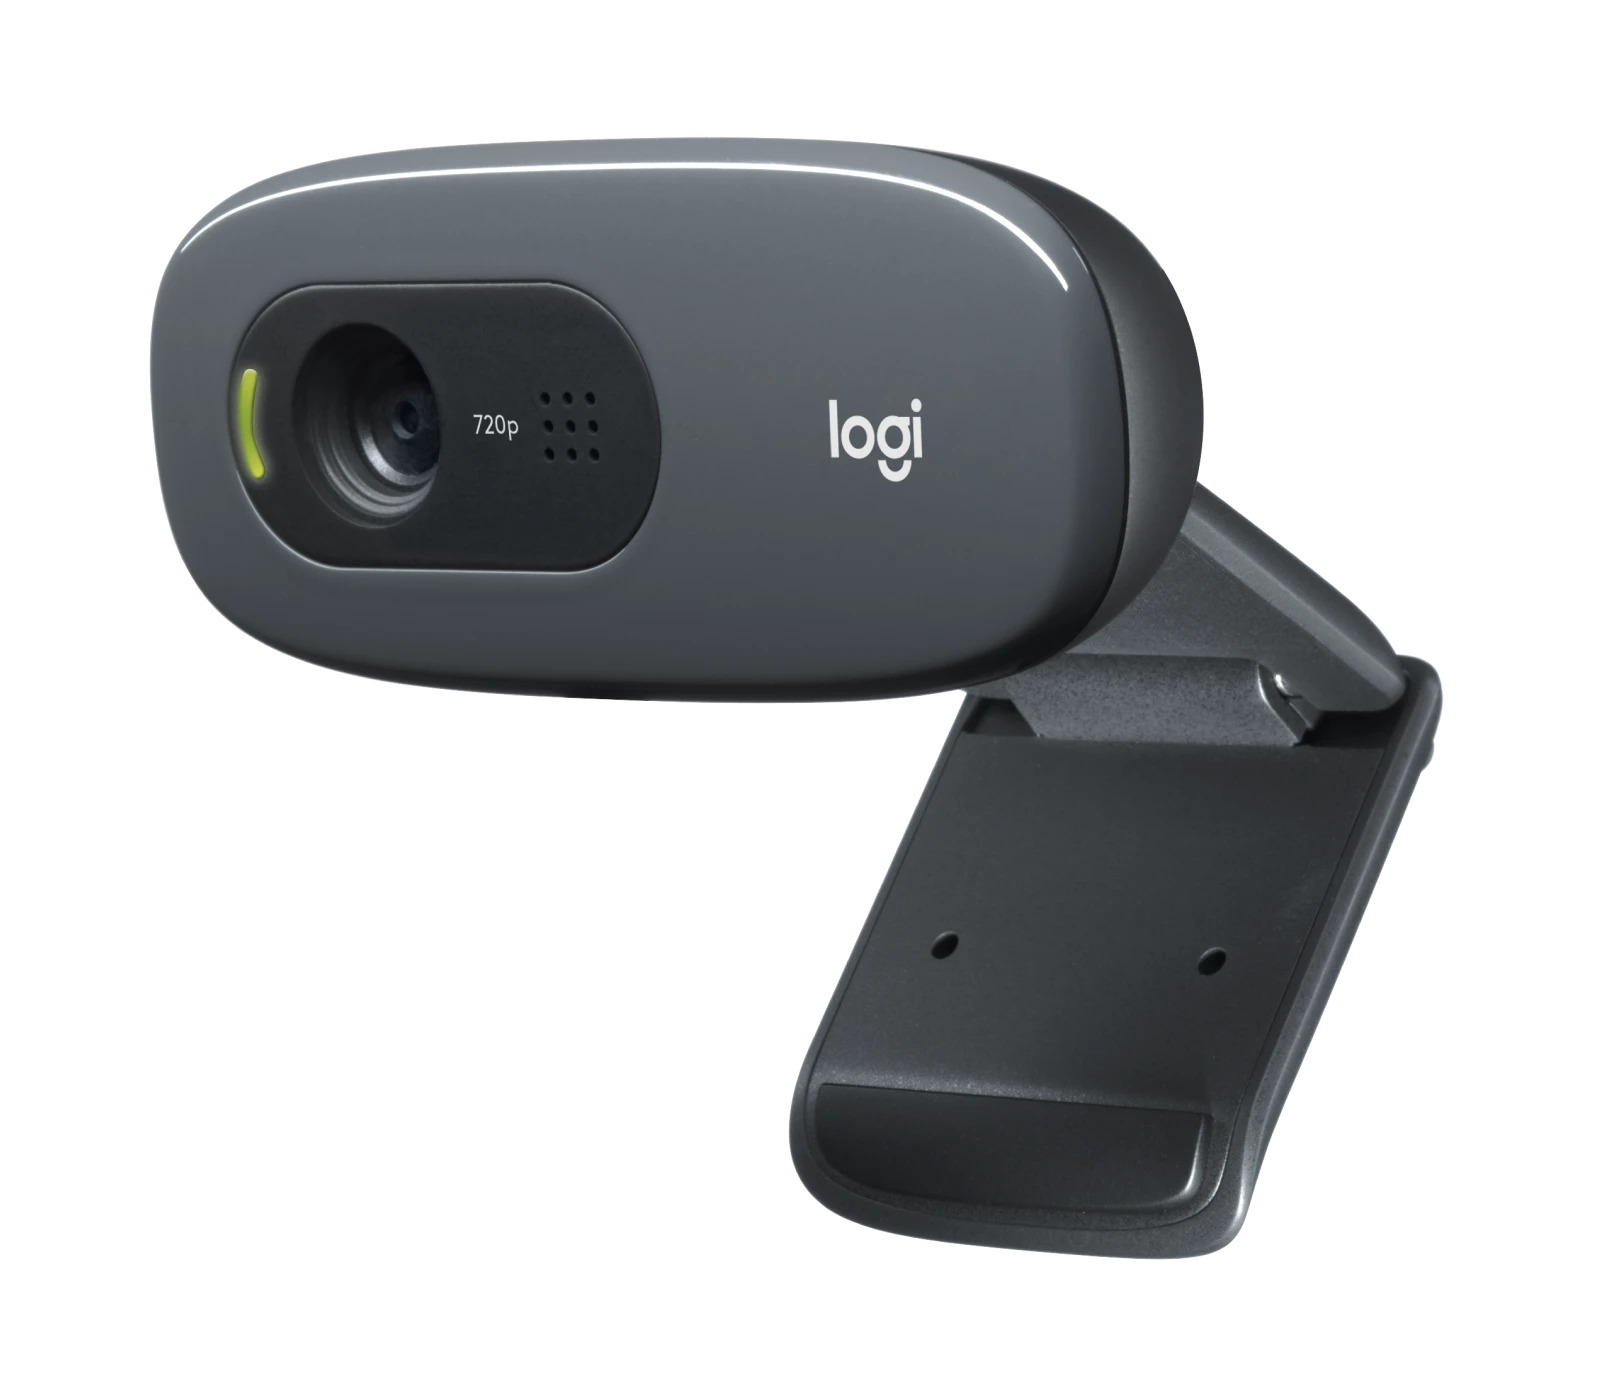
\includegraphics[scale=0.15]{img/webcamC270.jpg}
	\caption{Logitech HD Webcam C270 \cite{webcam}}
	\label{fig:webcam}
\end{figure}
La Logitech HD Webcam C270 es utilizada para capturar la foto de perfil de las personas que se registran en el sistema.
\subsection{Sensor QR}
\begin{figure}[H]
	\centering
	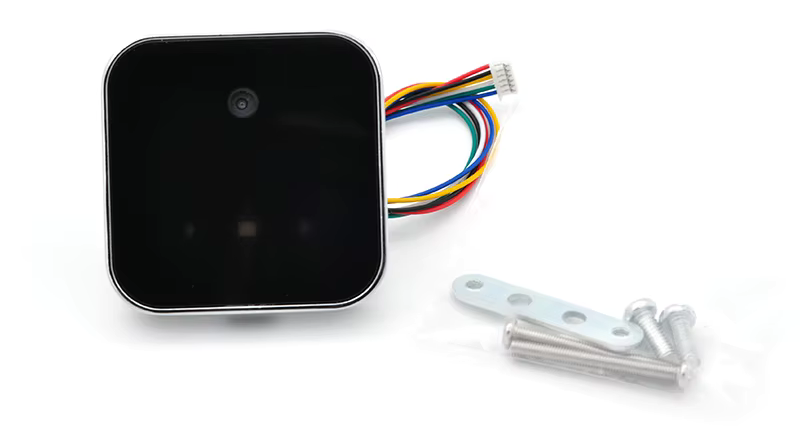
\includegraphics[scale=0.5]{img/SensorQR.png}
	\caption{Sensor QR GM811 \cite{GM811}}
	\label{fig:sensorQR}
\end{figure}
El sensor QR GM811 es utilizado para leer los códigos QR de las cedulas de identidad, de las personas que ingresan al laboratorio, permitiendo un registro rápido y eficiente de la asistencia.
\newparagraph
Lo más importante de este sensor es que tiene un modo de POS (Point of Sale) que permite leer códigos QR de manera rápida y eficiente, lo que lo hace ideal para el proyecto.

\newpage
\section{Documentación desarrollo del Software}
\subsection{Etapa 0}
Se elaboro de un informe para la asignatura Sistemas de Información, en el cual se desarrolló un prototipo de un sistema de asistencia digital para el Laboratorio de Sistemas Automatizados de Producción de la Universidad del Bío-Bío.
El software inicialmente fue desarrollado de forma rudimentaria, pues lo importante del informe era llevar a cabo una idea, definir ciertos aspectos y realizar los diagramas de contexto, nivel superior y de procedimientos administrativos.

\subsection{Etapa 1}
En esta etapa se utilizo la idea de la Etapa 0 para desarrollarlo en la practica profesional II dentro del Laboratorio de Sistemas Automatizados de Producción de la Universidad del Bío-Bío.
\newparagraph
Se utilizo inicialmente un dispositivo Windows con una cámara web para el registro de asistencia, el software ánalizaba la imagen con opencv y detectaba el código QR de la cédula de identidad, luego se enviaba la información a una base de datos en PostgreSQL.

\subsection{Etapa 2}
En esta etapa se utilizo una Raspberry Pi 4 con una cámara web, se utilizo el SO Raspbian y el mismo software de la etapa 1.
\newparagraph
Se observo que la Raspberry Pi 4 tenia problemas al procesar la imagen de la cámara web, tanto en la detección del código QR como en la velocidad de actualización de la imangen en la interfaz gráfica.
Al intentar resolver el problema, se crearon más problematicas, pues se intento implementar la pantalla tactil que se comunicaba por GPIO, lo que genero problematicas en la comunicación, dejando la pantalla en negro, por lo que se tuvo que reinstalar el SO.
\newparagraph
Finalmente se decidió cambiar el software de registro de asistencia y utilizar un Sensor QR.

\subsection{Etapa 3 (Sin pruebas)}
Se desarrollo desde cero, el software de registro de asistencia, implementando el sensor QR.
Lo malo es que mientras se descubria el funcionamiento del sensor, se configuro a un modo que solo aceptaba configuracion por comunicacion Serial, pero luego no era reconocido por ningun dispositivo. Lo que nos retraso en nuestro limitado tiempo.
\newparagraph
El supervisor nos recomendo hacer algunos avances sin realizar pruebas para entregar al menos una idea del software a implementar, para completar la practica profesional II.

\subsection{Etapa 4 (Sin pruebas)}
Se desarrollo una aplicación web para la visualización de los datos, para ello se utilizo Python con FastAPI. Para el acceso a esta aplicación, el supervisor debe acceder a la IP de las raspberry por el puerto 8000, la aplicación cuenta con un ingreso por PWT, para la seguridad mínima del sistema.
\newparagraph
Durante el desarrollo se fueron reformulando ciertas ideas, lo que llevo a algunas modificaciones de la BD, como por ejemplo la capacidad de notificar de un nuevo ingreso, la actualización automatica de la hora de salida si es que una persona no hubiera marcado y la actualización automatica de la zona horaria para inverno/verano.
\newparagraph
Al final de esta etapa se decidió utilizar Docker para contener los diferentes módulos del SW, aparte de su facil implementación, pues con el docker compose se puede crear facilmente una DB segura y compacta.

\section{Implementación}

\subsection{Software consultor}
\subsubsection{Librerías}
\begin{figure}[H]
	\centering
	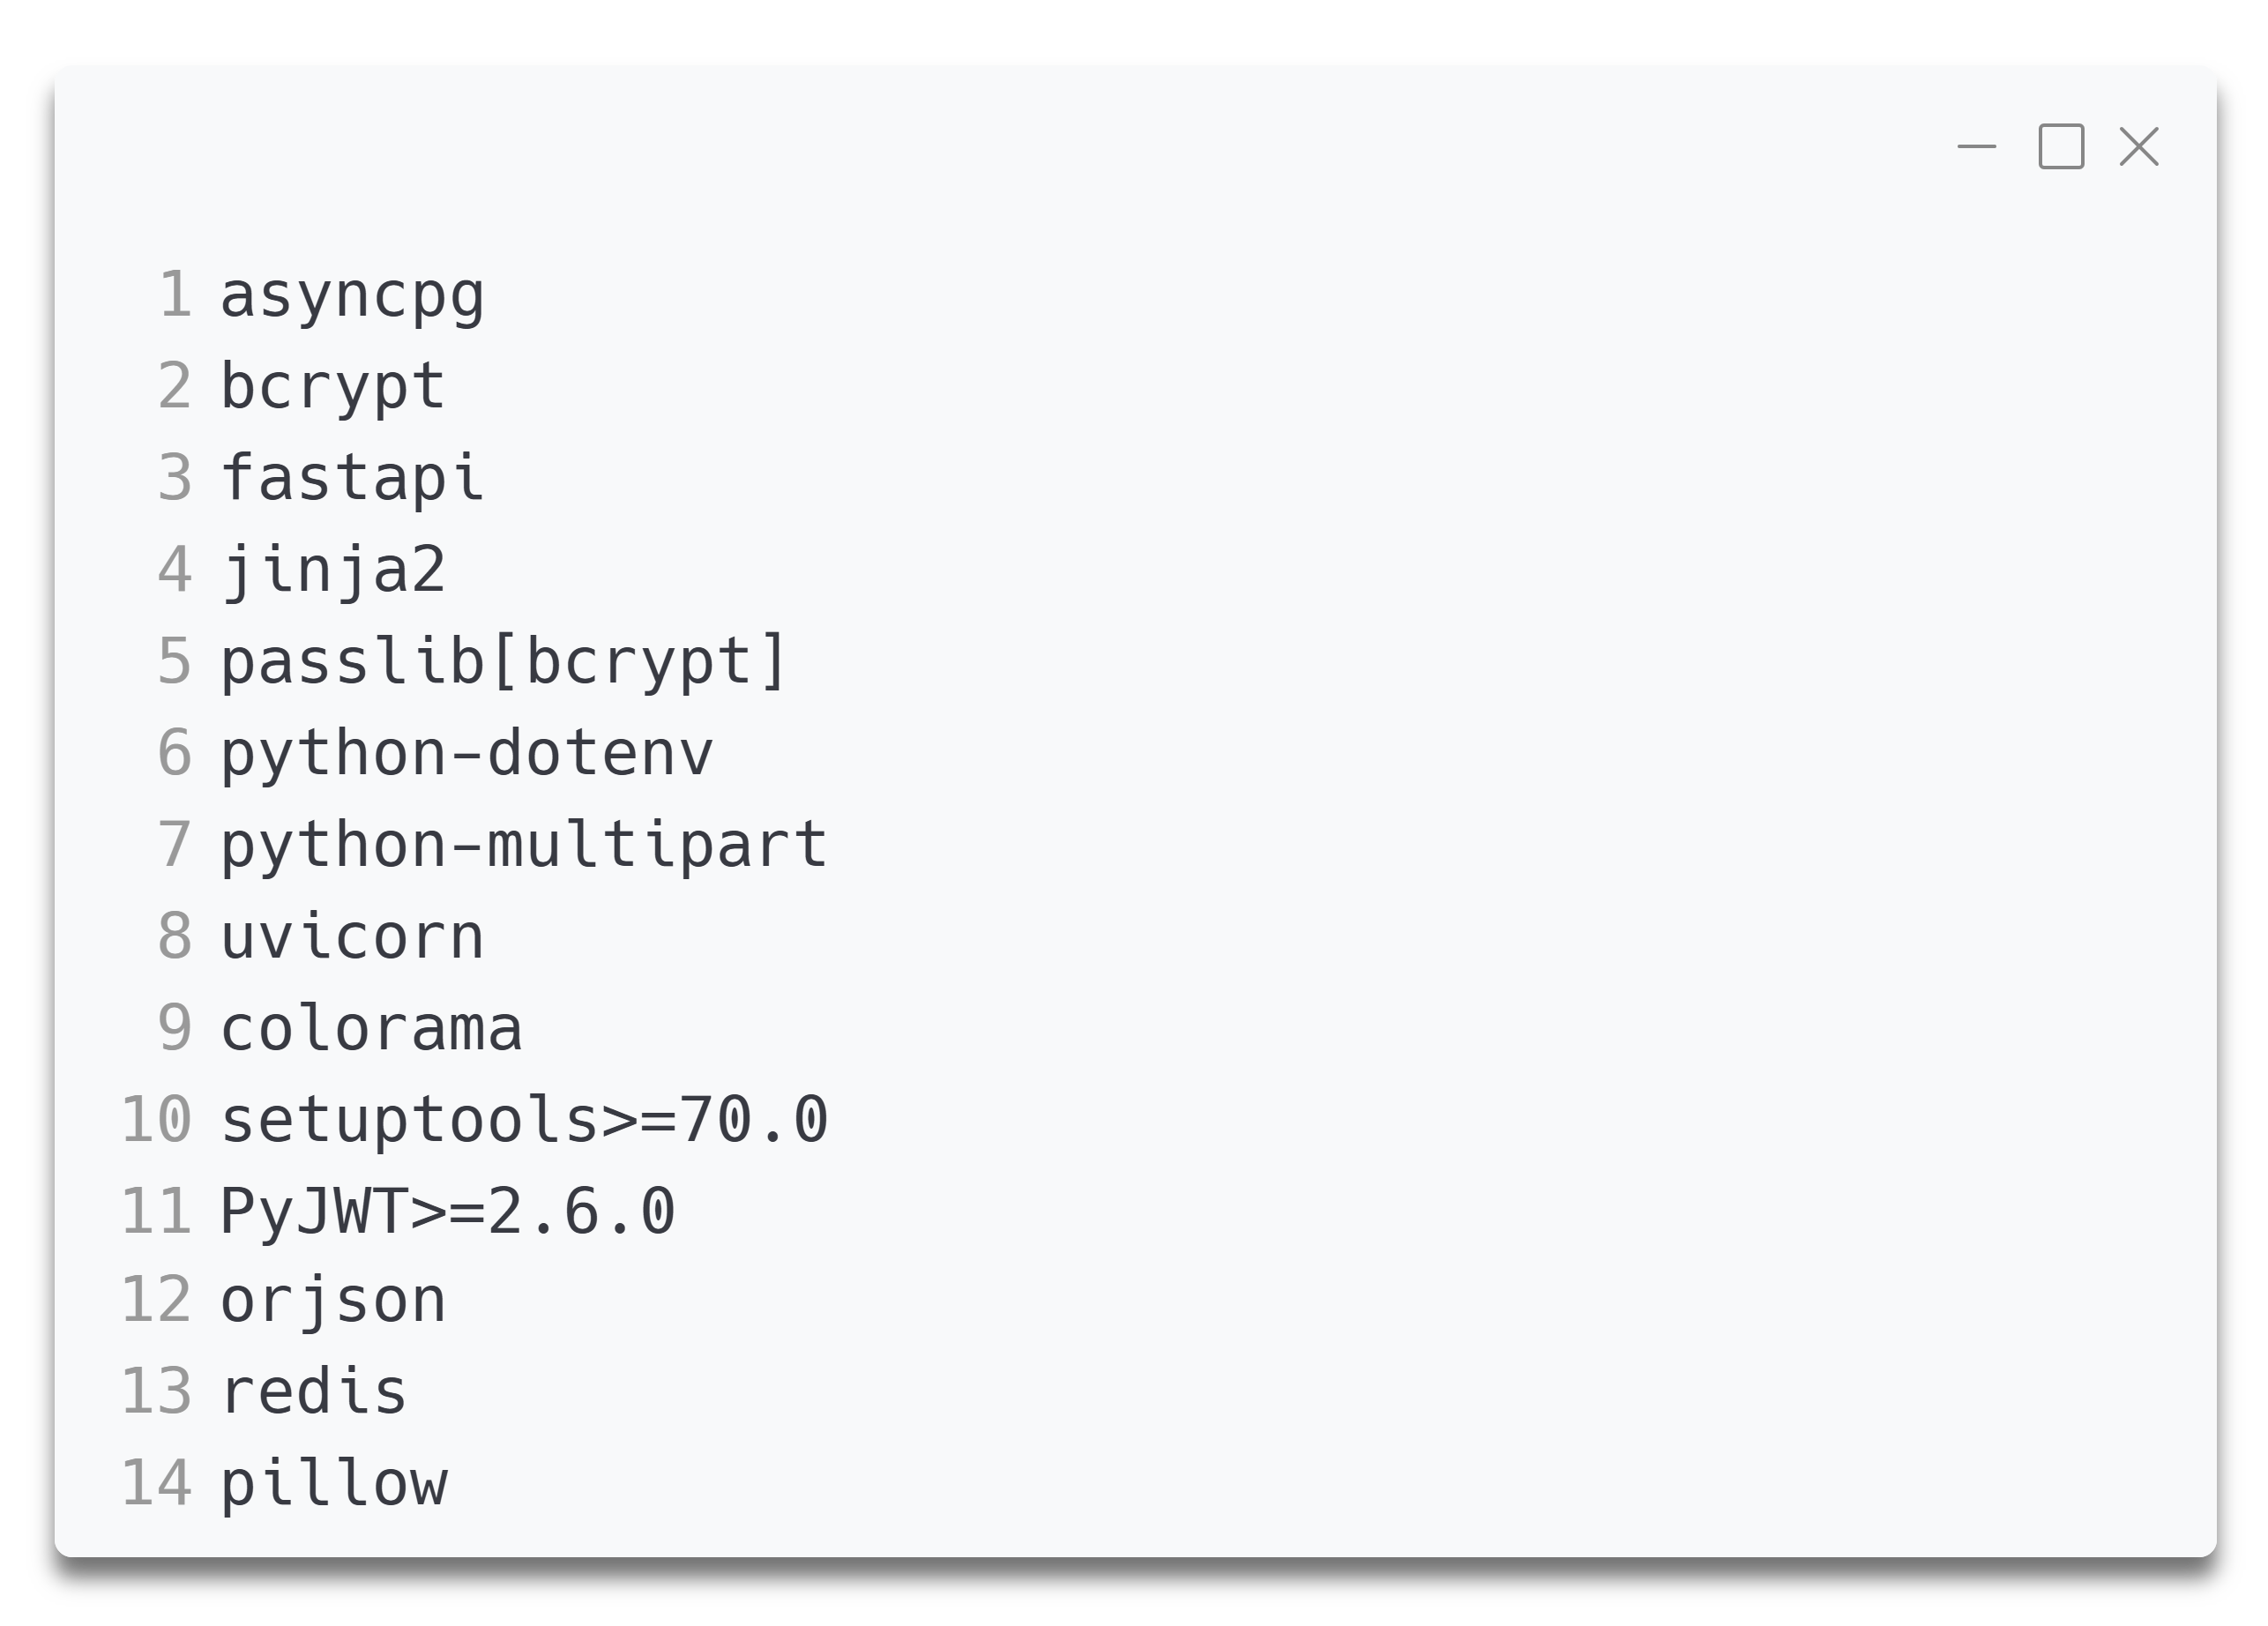
\includegraphics[scale=0.15]{img/requerimientosApp.png}
	\caption{Requerimientos software consultor}
	\label{fig:softwareConsultor}
\end{figure}
\subsubsection{Estructura de archivos y directorios}
\begin{figure}[H]
	\centering
	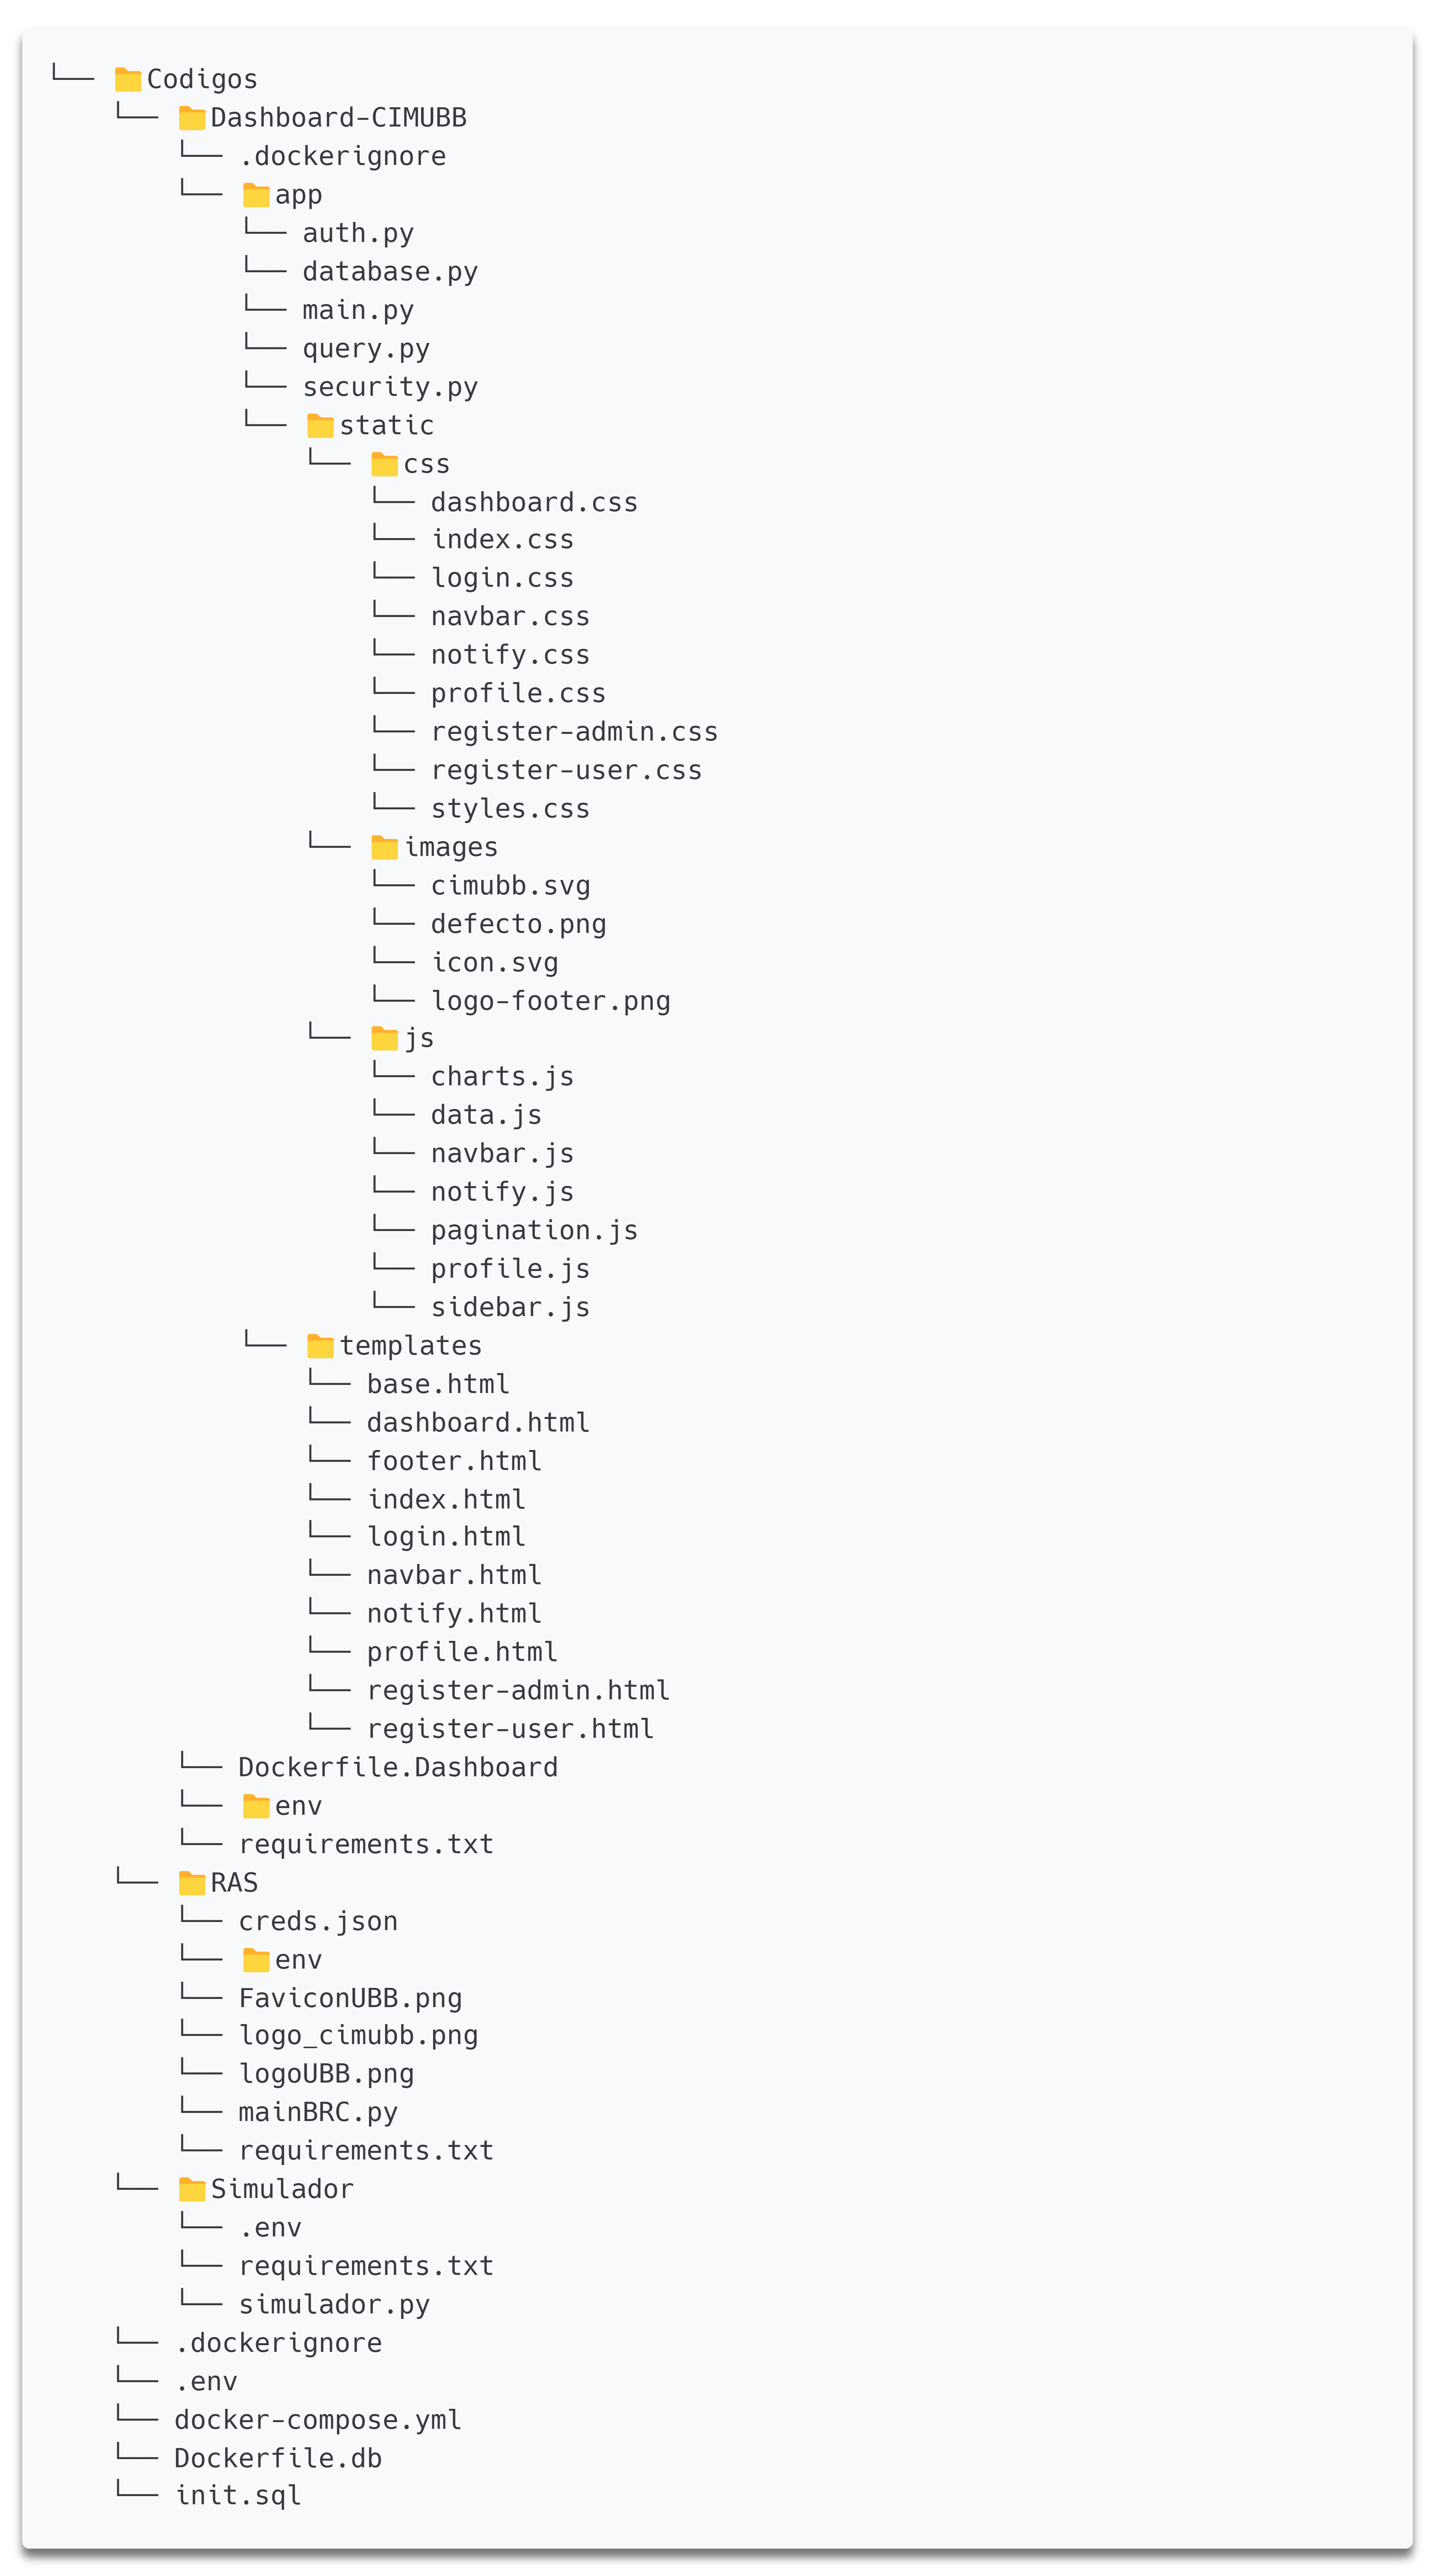
\includegraphics[scale=0.09]{img/estructuraDirectorio.png}
	\caption{Estructura de archivos y directorios}
	\label{fig:estructuraDirectorio}
\end{figure}
\subsubsection{Puesta en marcha (MANUAL)}
\textbf{WINDOWS}
\begin{enumerate}
	\item Clonamos el repositorio:
	      \newline
	      \begingroup
	      \centering
	      
\includegraphics[scale=0.1]{img/repositorioClone.png}
	      \endgroup

	\item Nos movemos a la carpeta del proyecto:
	      \newline
	      \begingroup
	      \centering
	      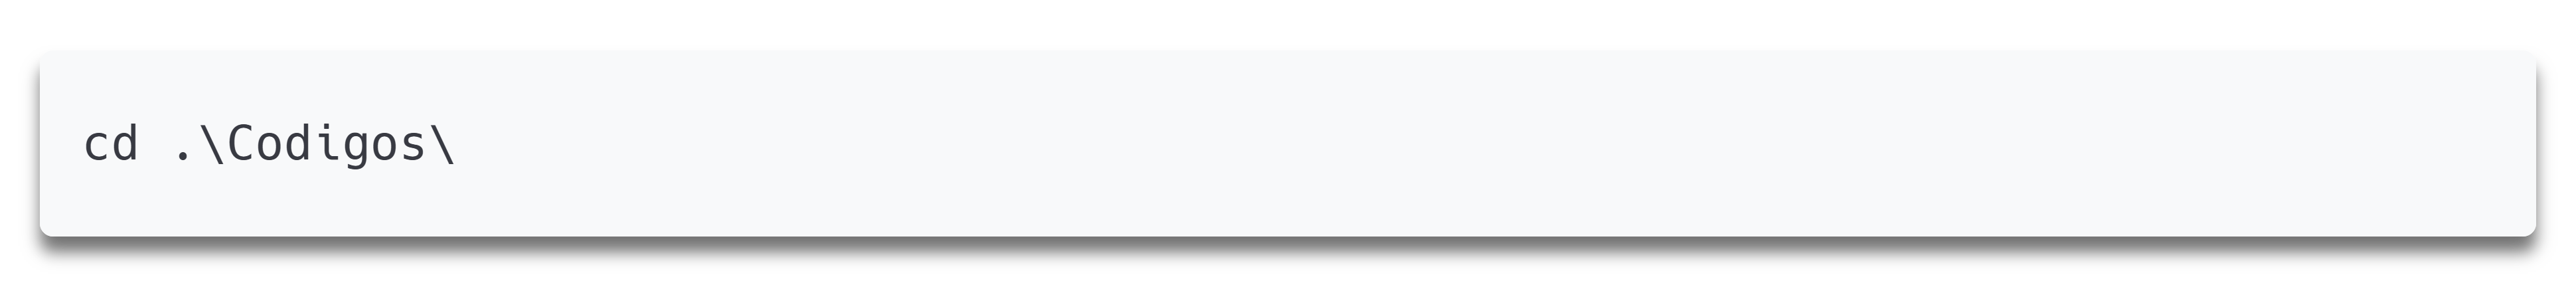
\includegraphics[scale=0.1]{img/mvCodigos.png}
	      \endgroup

	\item Utilizando PgAdmin 4, DBeaver o la conexión por terminal, creamos una base de datos en PostgreSQL con el nombre $cimubb\_asistencia$.
	      \begin{enumerate}
		      \item Crear la base de datos con el comando:
		            \newline
		            \begingroup
		            \centering
		            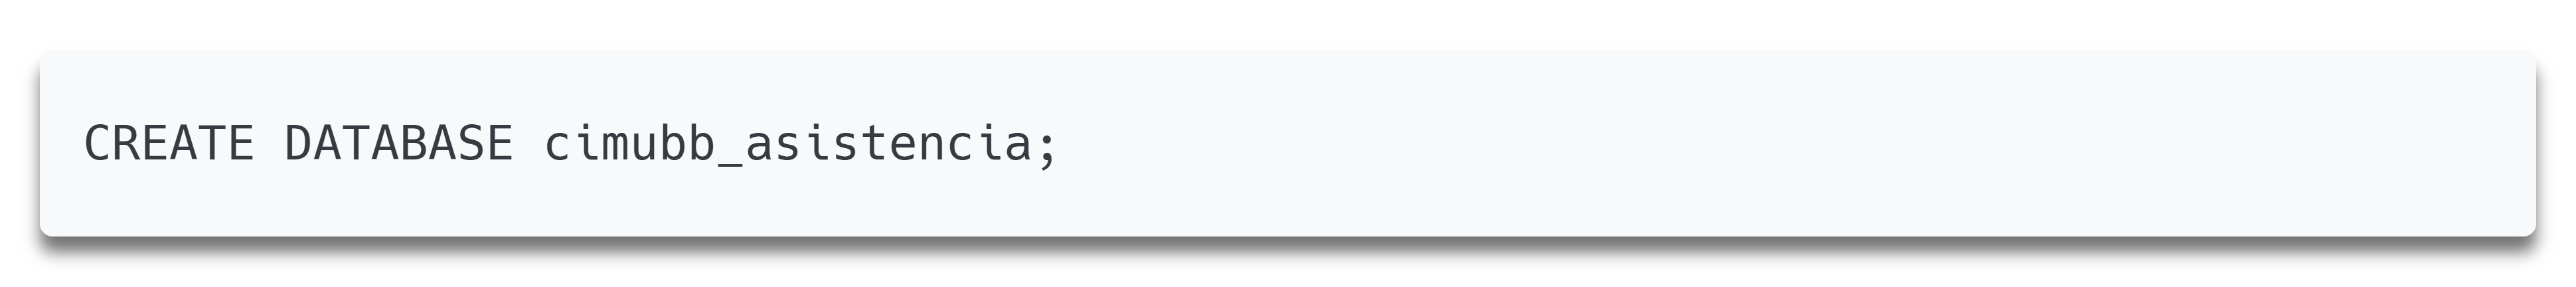
\includegraphics[scale=0.1]{img/sqlDB.png}
		            \endgroup

		      \item Nos conectamos a la BD creada:
		            \newline
		            \begingroup
		            \centering
		            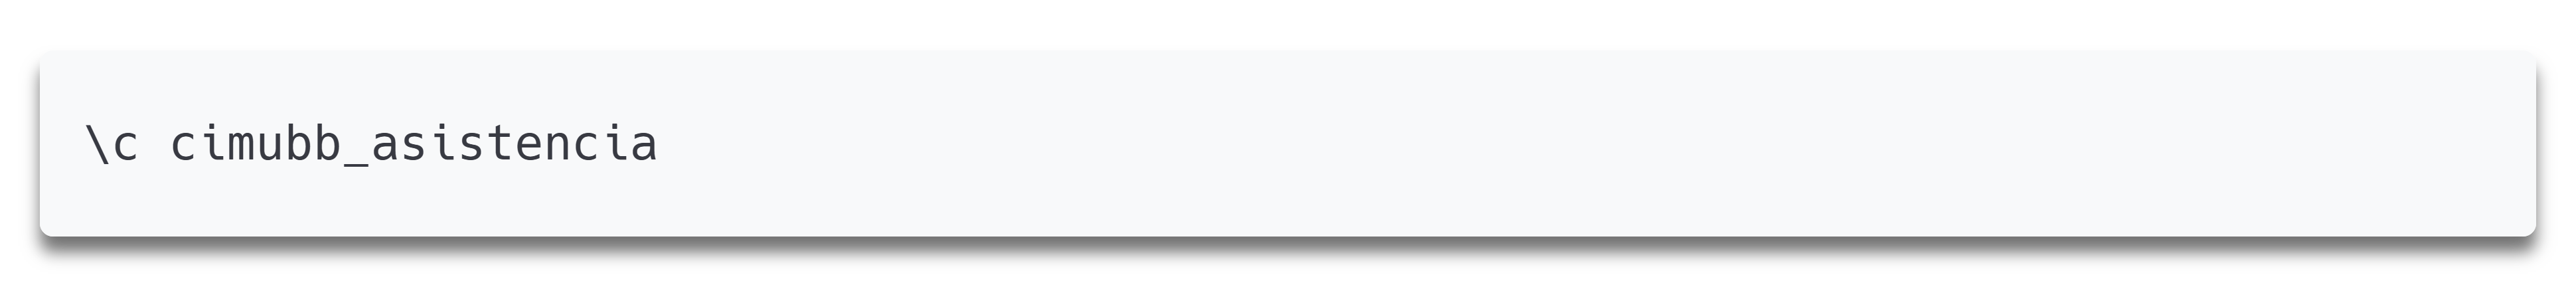
\includegraphics[scale=0.1]{img/sqlConnect.png}
		            \endgroup

		            \newpage
		            \textbf{Forma automática:}
		      \item Ejecutamos el archivo init.sql, utilizando la ruta del archivo. Como cron no existe para windows las tareas de marcar salida y actualizar zona horaria no funcionaran:
		            \newline
		            \begingroup
		            \centering
		            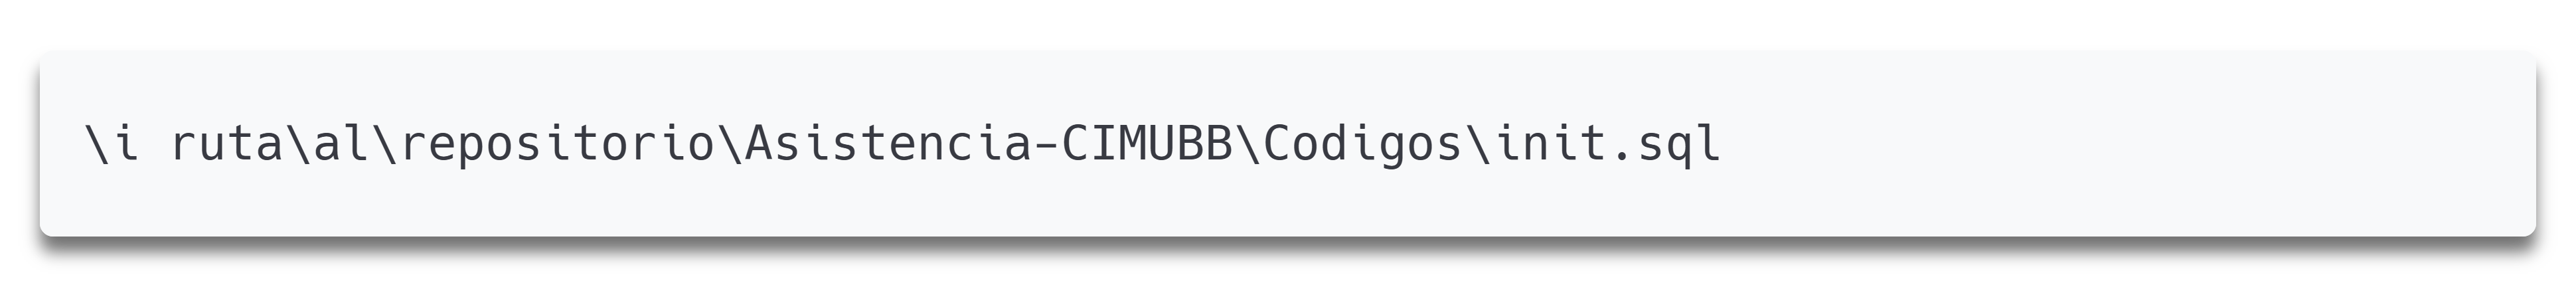
\includegraphics[scale=0.1]{img/sqlAutomatico.png}
		            \endgroup
		            \newline
		            \textbf{Forma manual:}
		      \item Creamos las tablas:
		            \newline
		            \begingroup
		            \centering
		            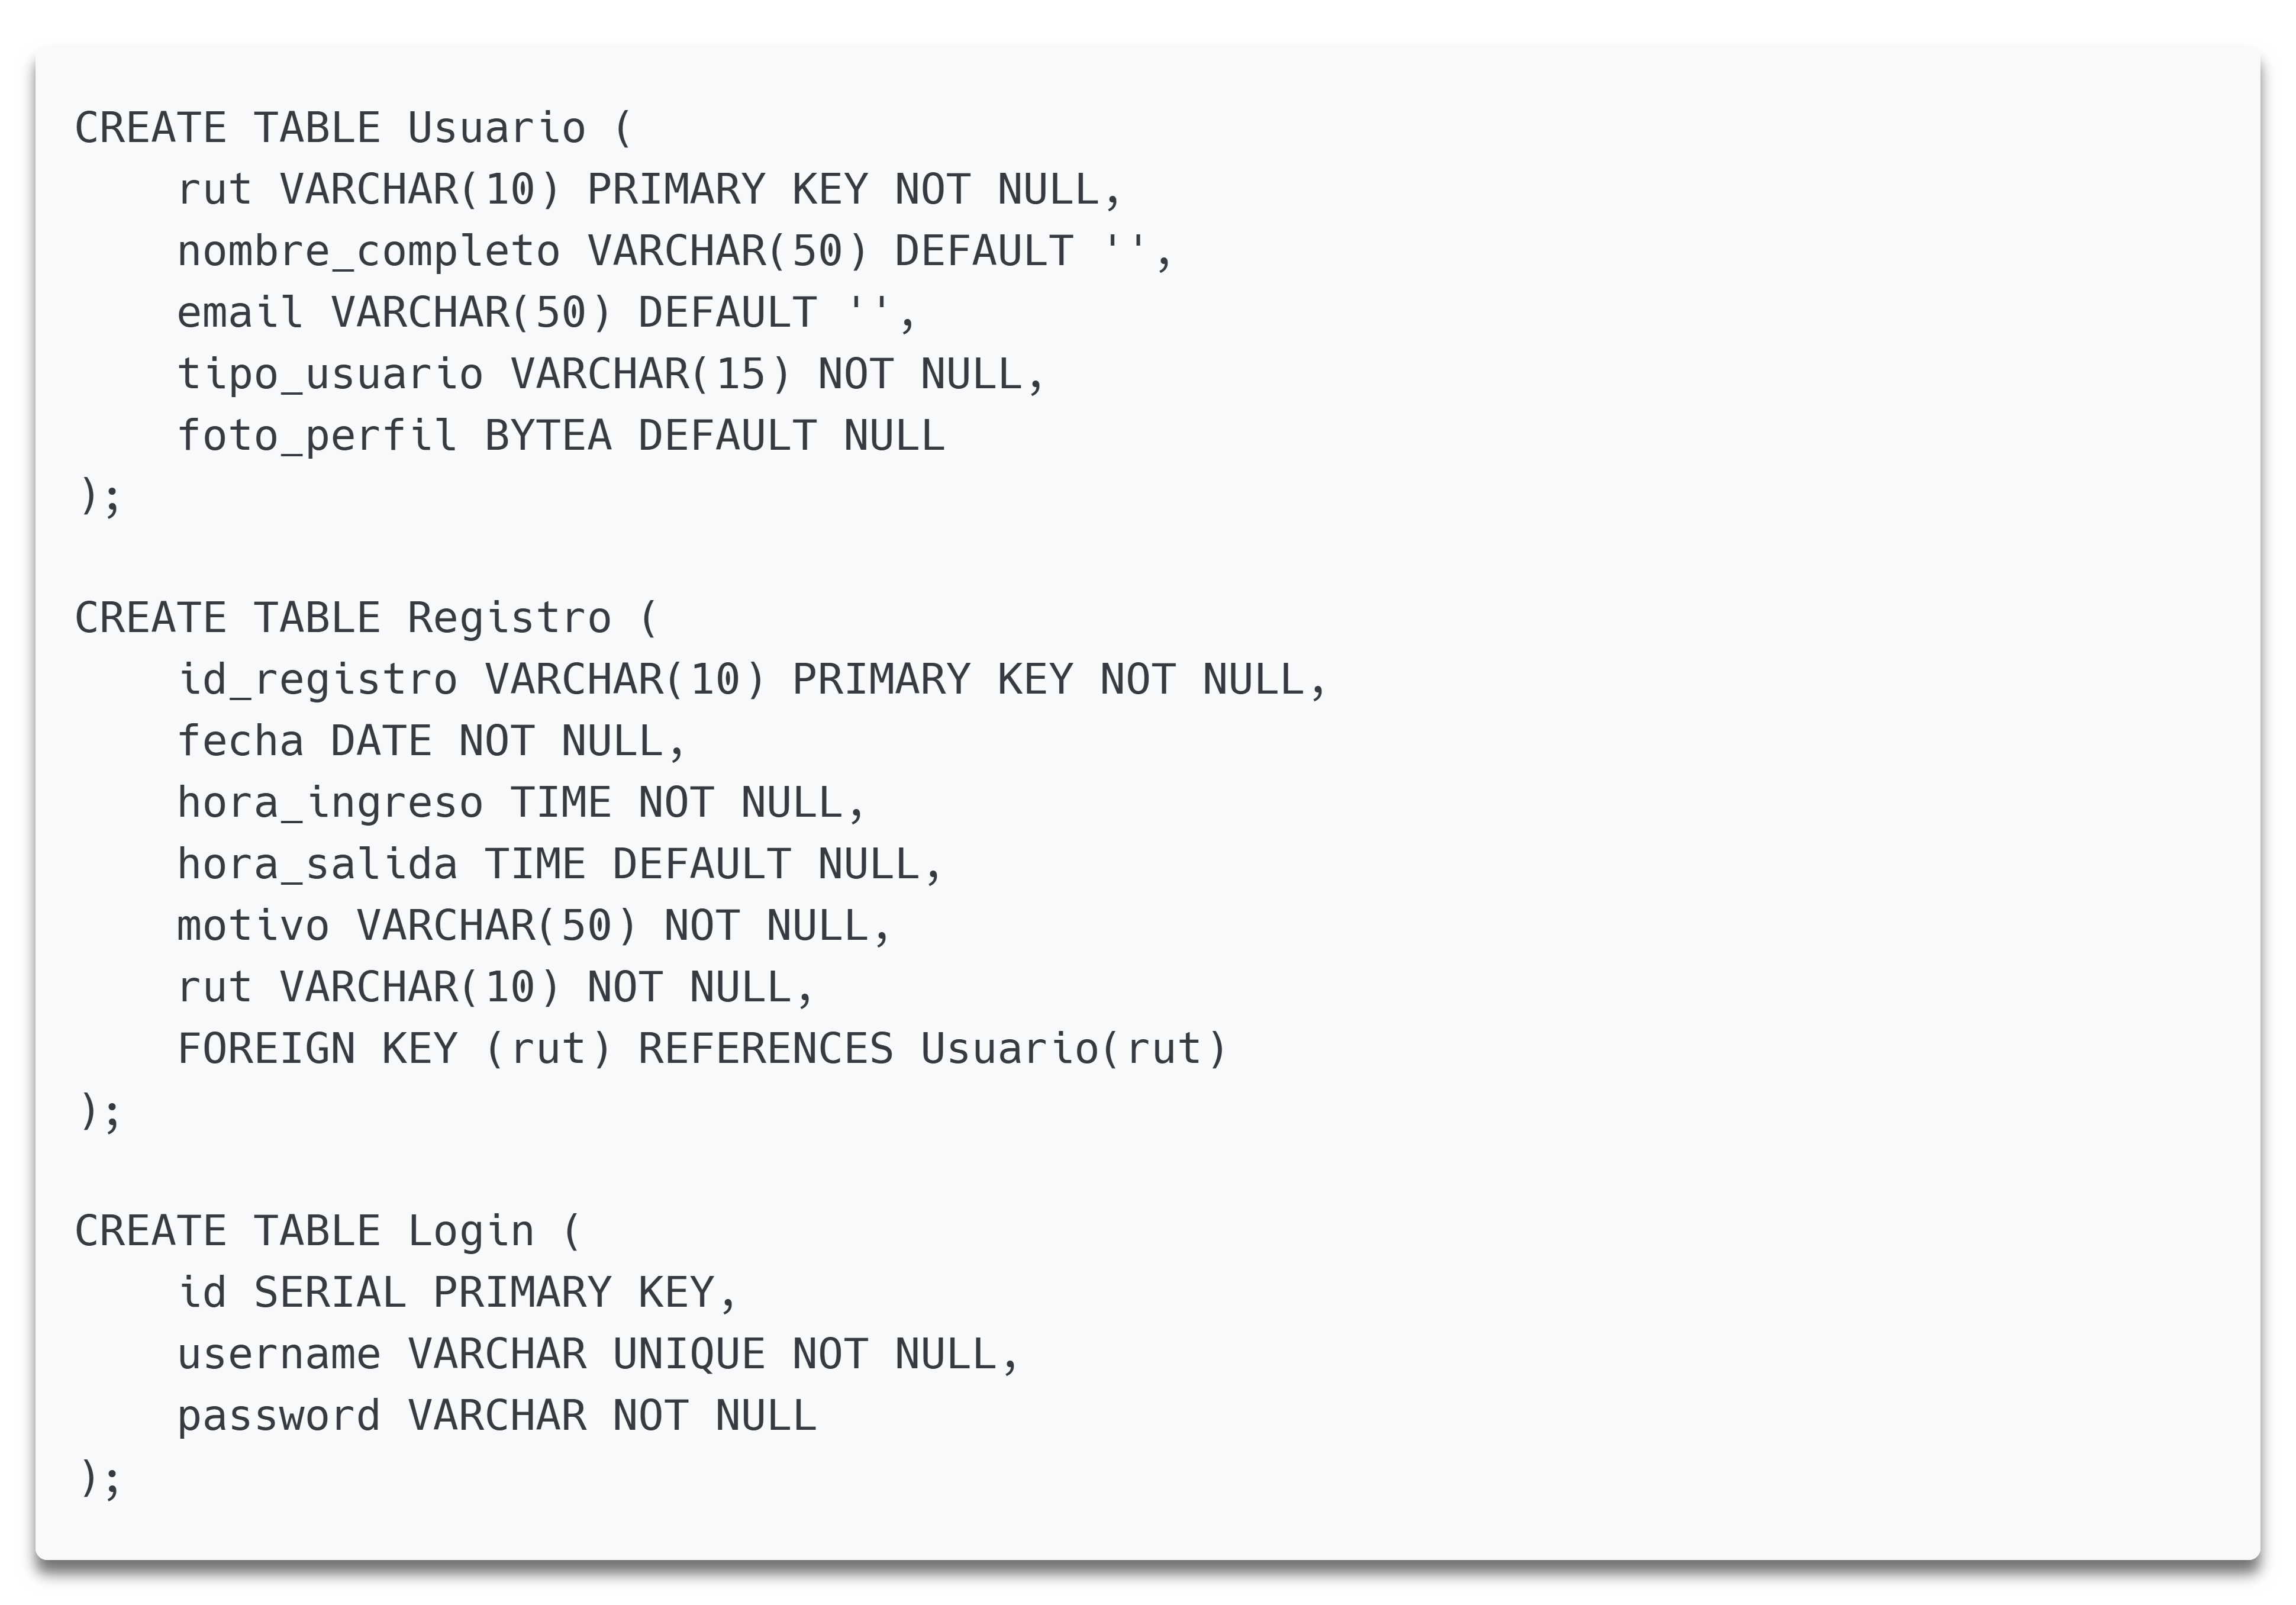
\includegraphics[scale=0.1]{img/sqlTablas.png}
		            \endgroup

		      \item Habilitamos la extensión crypto e insertamos el login para el admin:
		            \newline
		            \begingroup
		            \centering
		            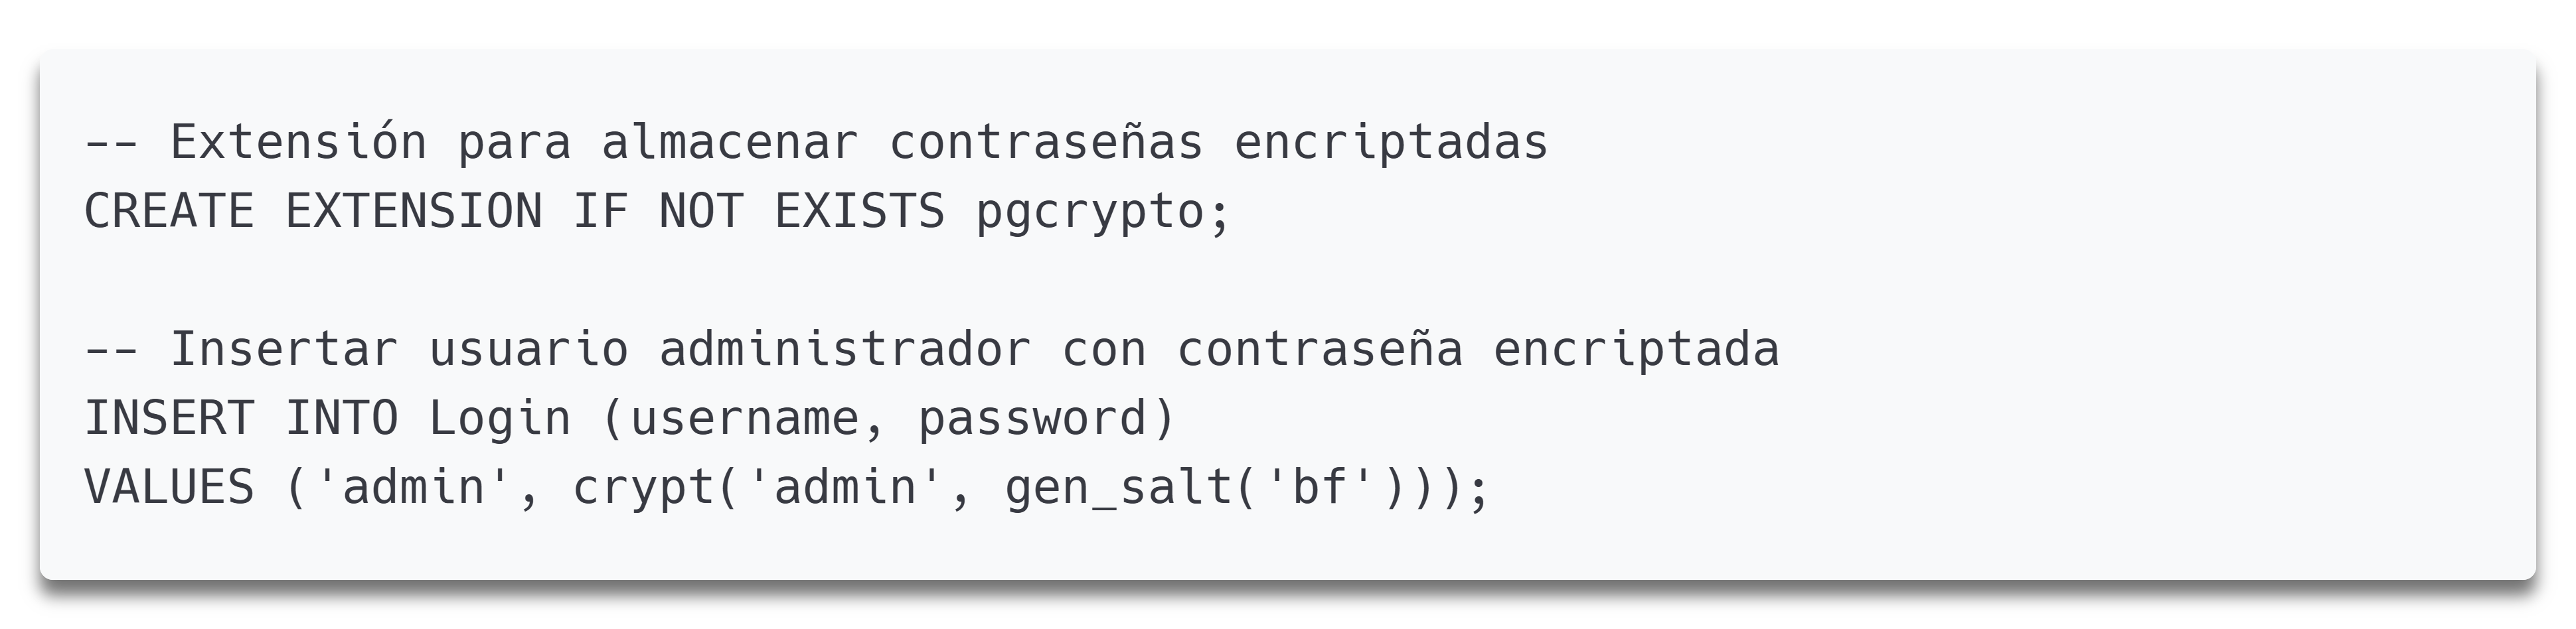
\includegraphics[scale=0.1]{img/sqlCryptoYAdmin.png}
		            \endgroup
		            \newline
		            \textbf{*OBS:} Por obvias razones se recomienda cambiar el username y el password del login a la dashboard.

		            \newpage
		      \item Habilitamos la extensión cron y creamos una función para marcar la salida automatica a las 19:00 de los registros que se les olvido marcar la hora salida:
		            \newline
		            \begingroup
		            \centering
		            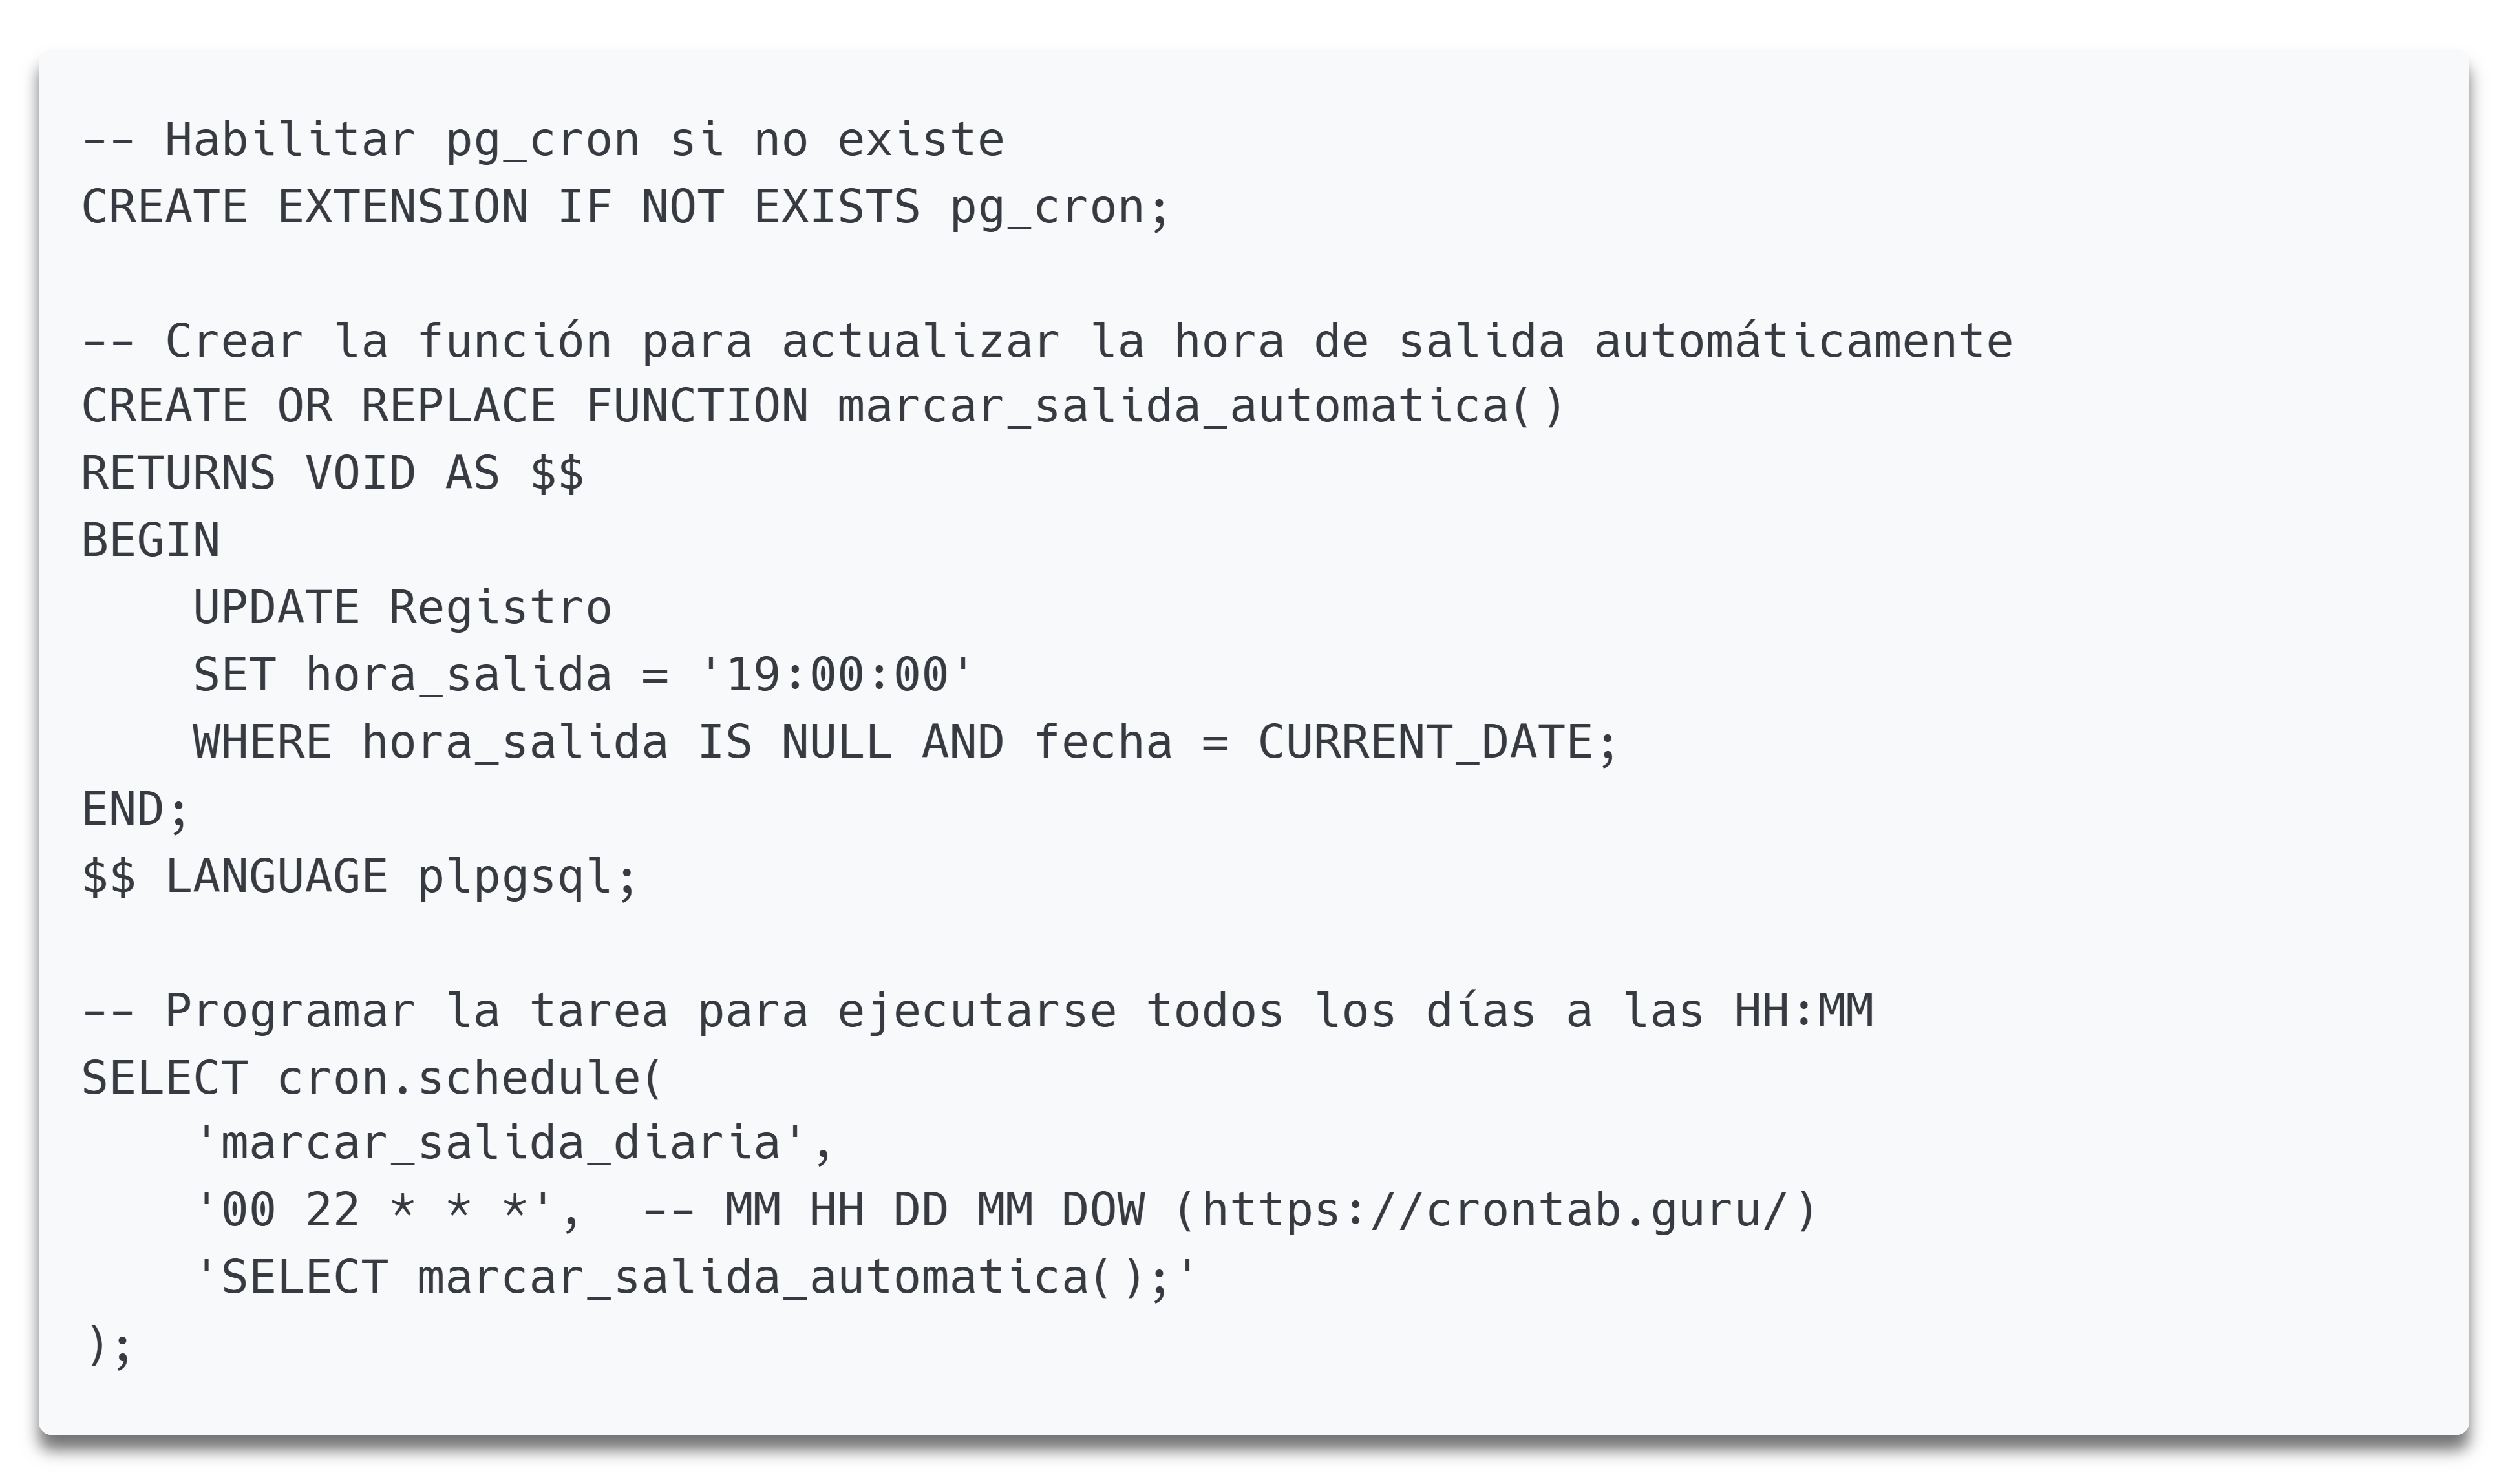
\includegraphics[scale=0.1]{img/sqlCronSalidaAuto.png}
		            \endgroup
		      \item Creamos una función para habilitar un LISTEN / NOTIFY con un trigger al detectar un ingreso o salida:
		            \newline
		            \begingroup
		            \centering
		            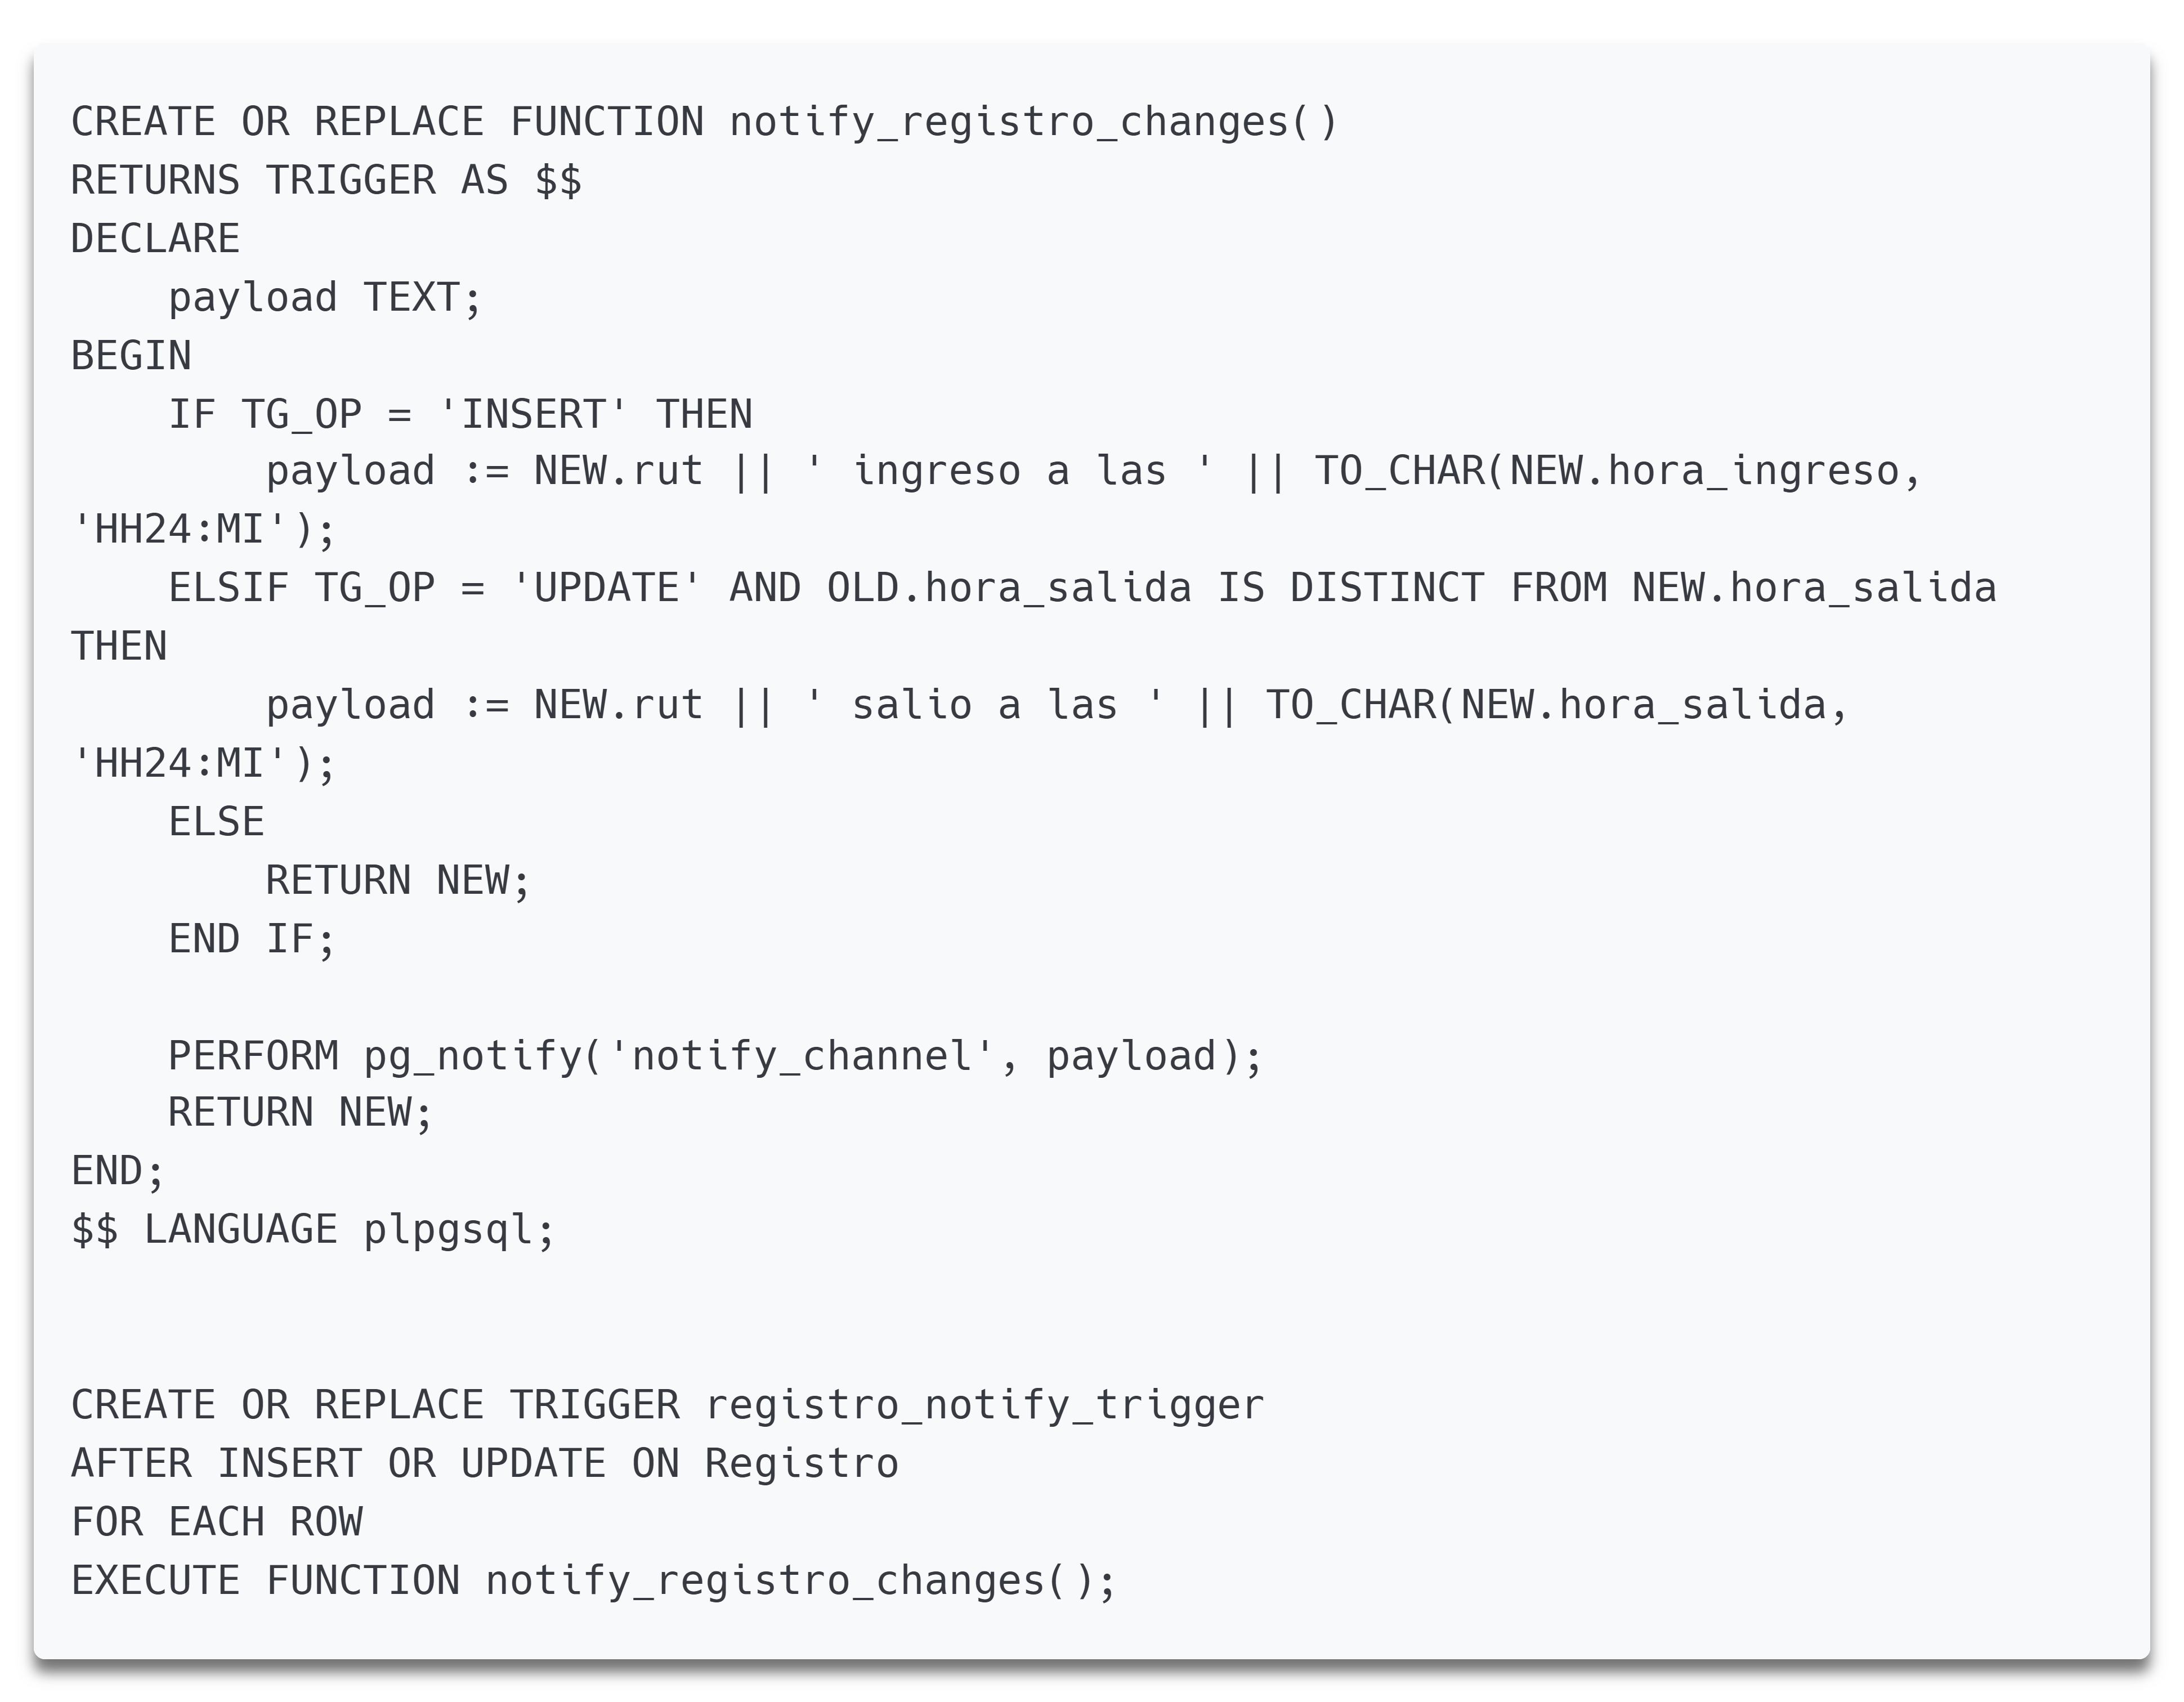
\includegraphics[scale=0.1]{img/sqlTrigger.png}
		            \endgroup
		            \newpage
		      \item Creamos una función para actualizar la zona horaria, pues postgres trabaja con UTC:
		            \newline
		            \begingroup
		            \centering
		            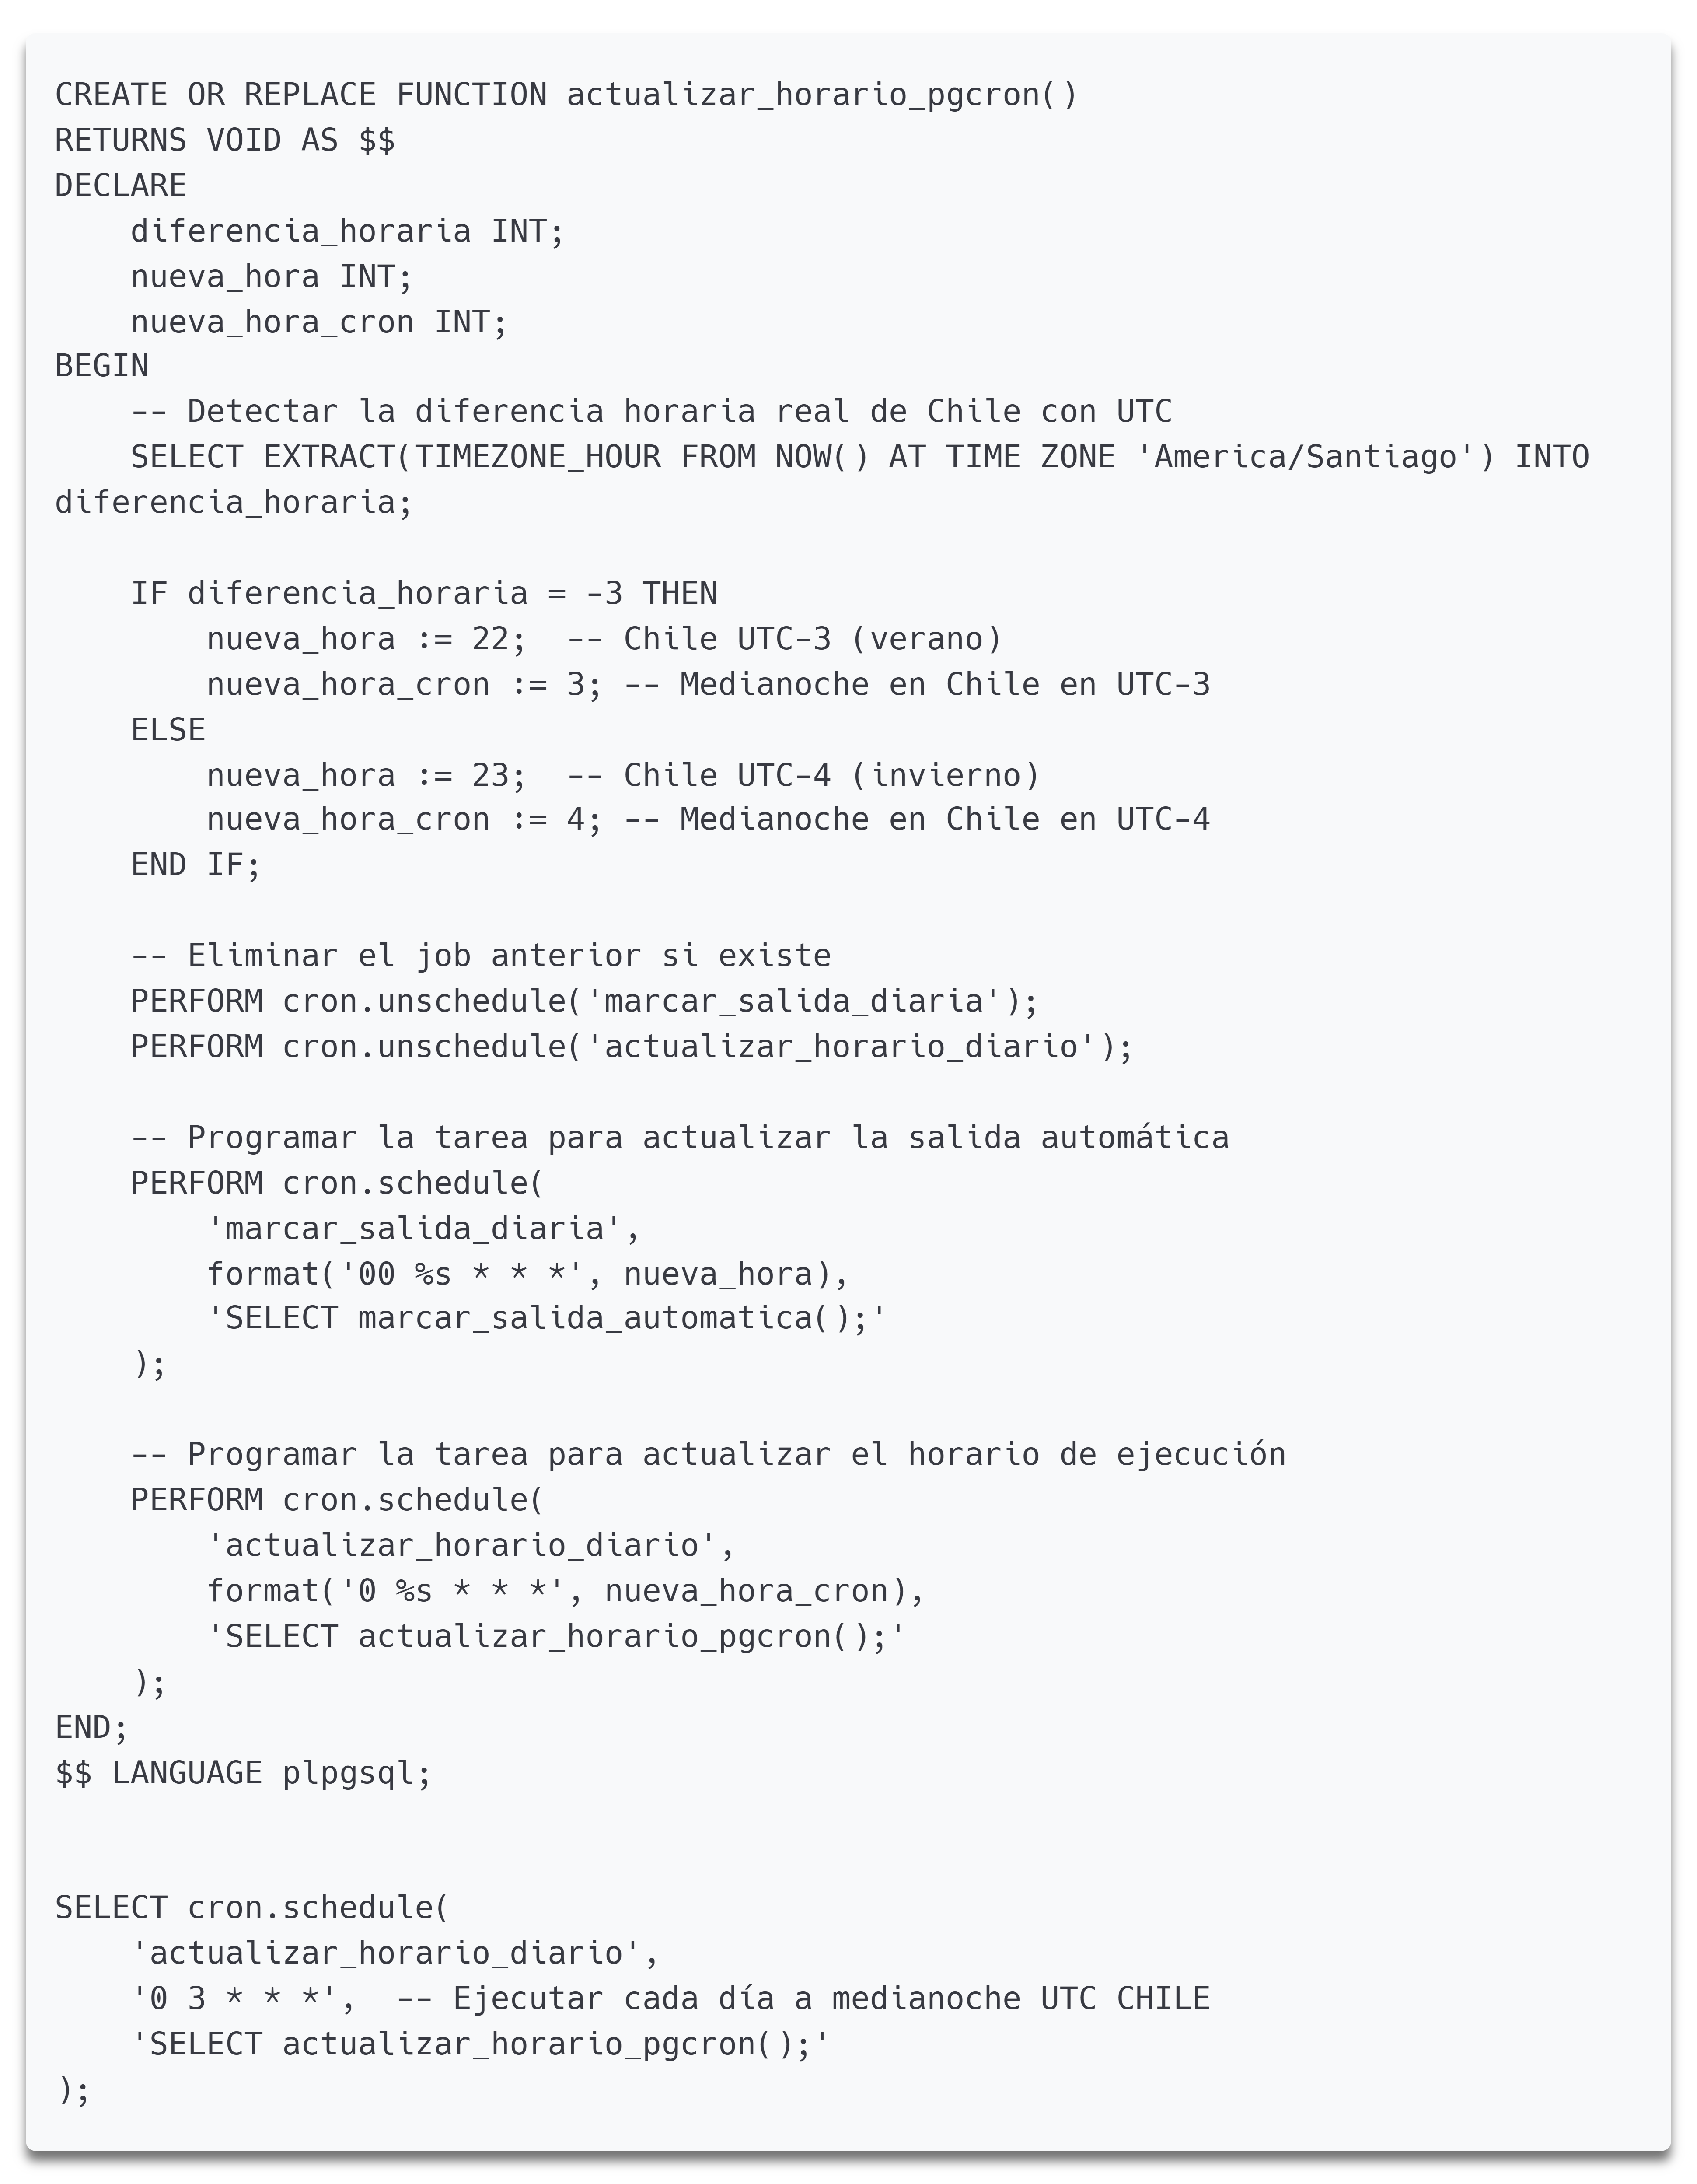
\includegraphics[scale=0.1]{img/sqlCronZonaHoraria.png}
		            \endgroup
		            \newline
		            *OBS: El paso g) y h) no funcionaran porque CRON no existe para Windows, por lo que estas funciones no aplican, pues el software fue desarrollado para raspberryPi.
	      \end{enumerate}

	\item Volviendo al repositorio nos movemos a la carpeta Dashboard:
	      \newline
	      \begingroup
	      \centering
	      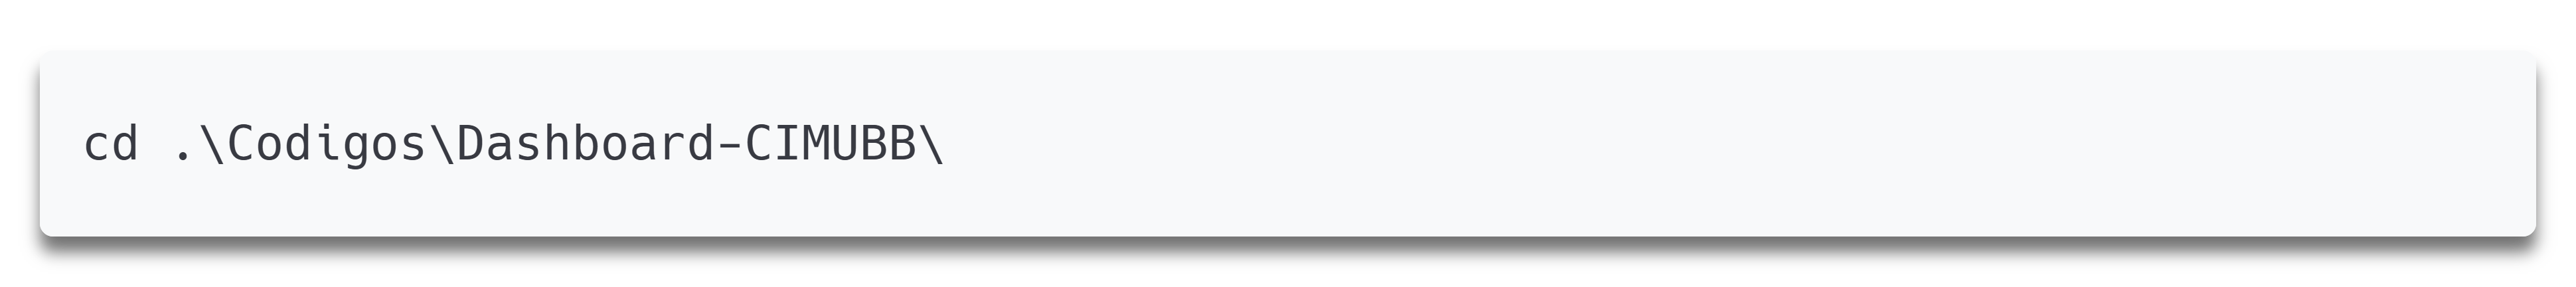
\includegraphics[scale=0.1]{img/mvDashboard.png}
	      \endgroup
	      \newpage
	\item Creamos un entorno virtual de python y lo activamos:
	      \newline
	      \begingroup
	      \centering
	      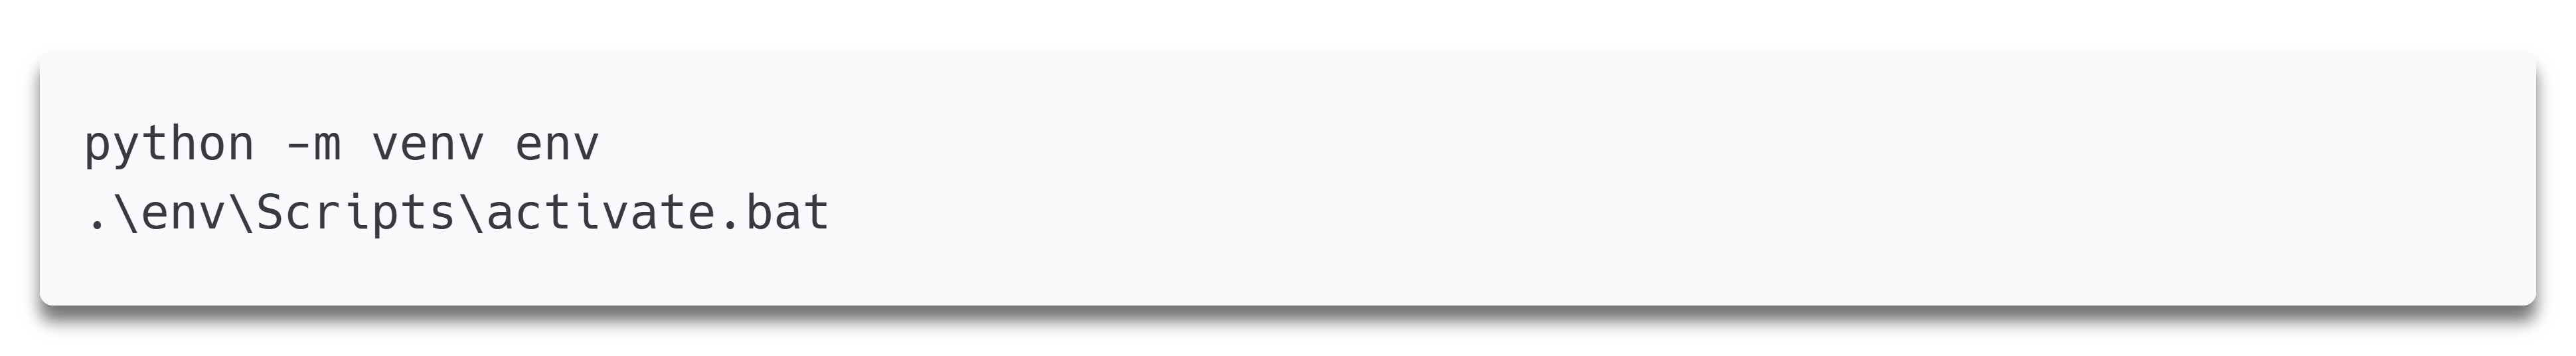
\includegraphics[scale=0.1]{img/pythonVirtual.png}
	      \endgroup

	\item Instalamos las dependencias:
	      \newline
	      \begingroup
	      \centering
	      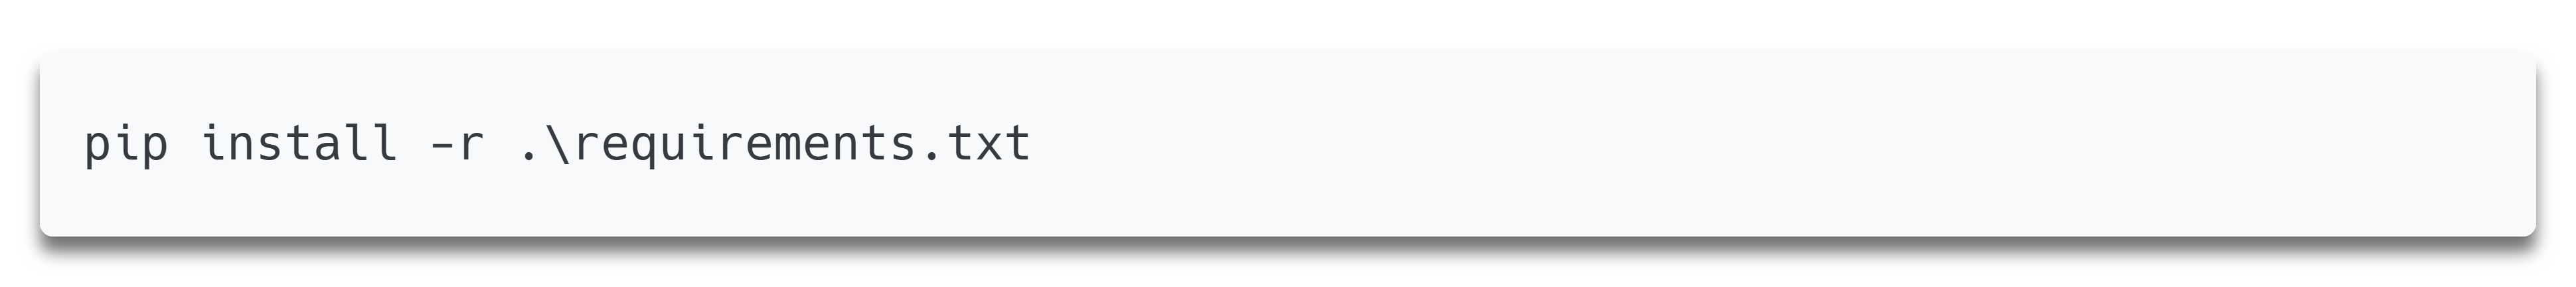
\includegraphics[scale=0.1]{img/pipRequerements.png}
	      \endgroup
	\item Configuramos el archivo .env dentro de la carpeta Dashboard-CIMUBB con las siguientes variables:
	      \newline
	      \begingroup
	      \centering
	      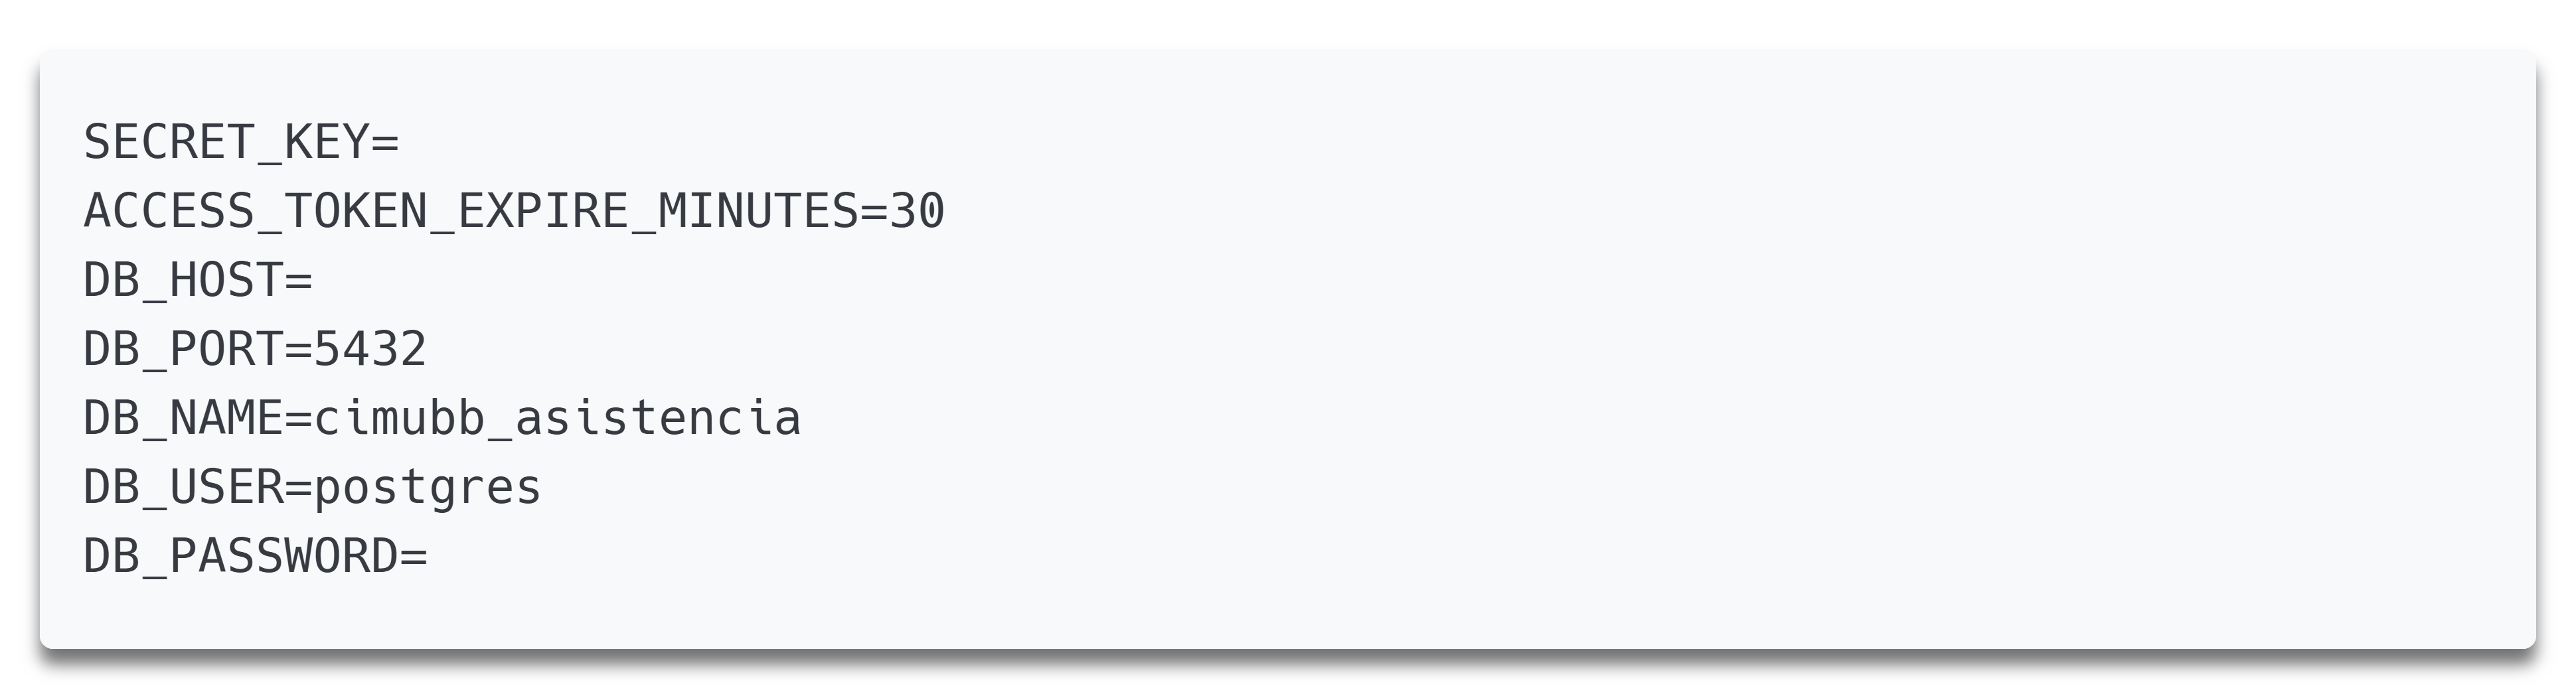
\includegraphics[scale=0.1]{img/dotenv.png}
	      \endgroup
	      \newline
	      \textbf{*OBS:} Para la generación del SECRET\_KEY utilizaremos la pagina browserling\cite{randomString}
	      \begin{figure}[H]
		      \centering
		      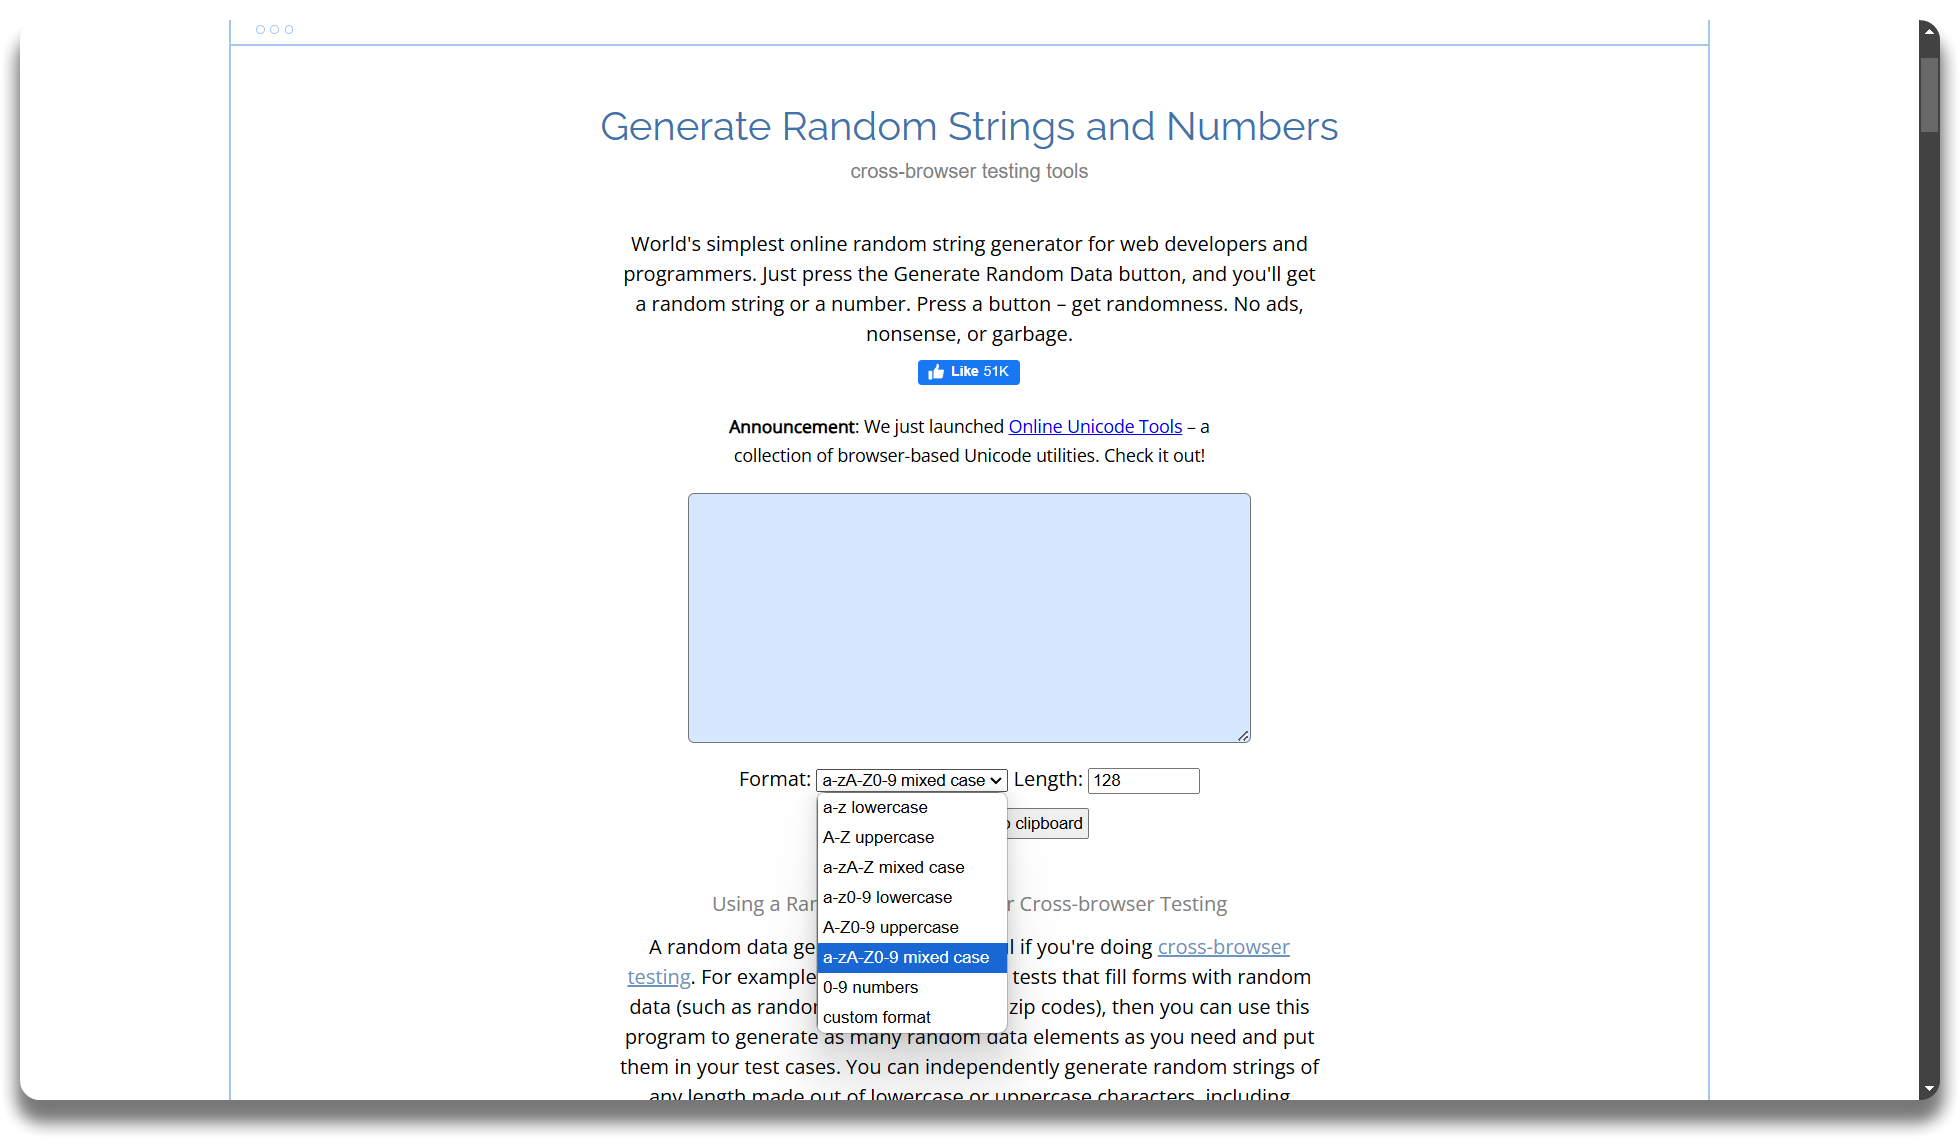
\includegraphics[scale=0.31]{img/capturaRandomString.png}
		      \caption{Generate Random Strings and Numbers \cite{randomString}}
		      \label{fig:randomString}
	      \end{figure}

	\item Para finalizar ejecutamos el servidor de UVICORN:
	      \newline
	      \begingroup
	      \centering
	      
\includegraphics[scale=0.1]{img/uvicorn.png}
	      \endgroup
\end{enumerate}

\newpage
\subsubsection{Puesta en marcha (AUTOMÁTICA)}
\textbf{DOCKER}
\begin{enumerate}
	\item Teniendo instalado docker, clonamos el repositorio:
	      \newline
	      \begingroup
	      \centering
	      
\includegraphics[scale=0.1]{img/repositorioClone.png}
	      \endgroup

	\item Nos movemos a la carpeta del proyecto:
	      \newline
	      \begingroup
	      \centering
	      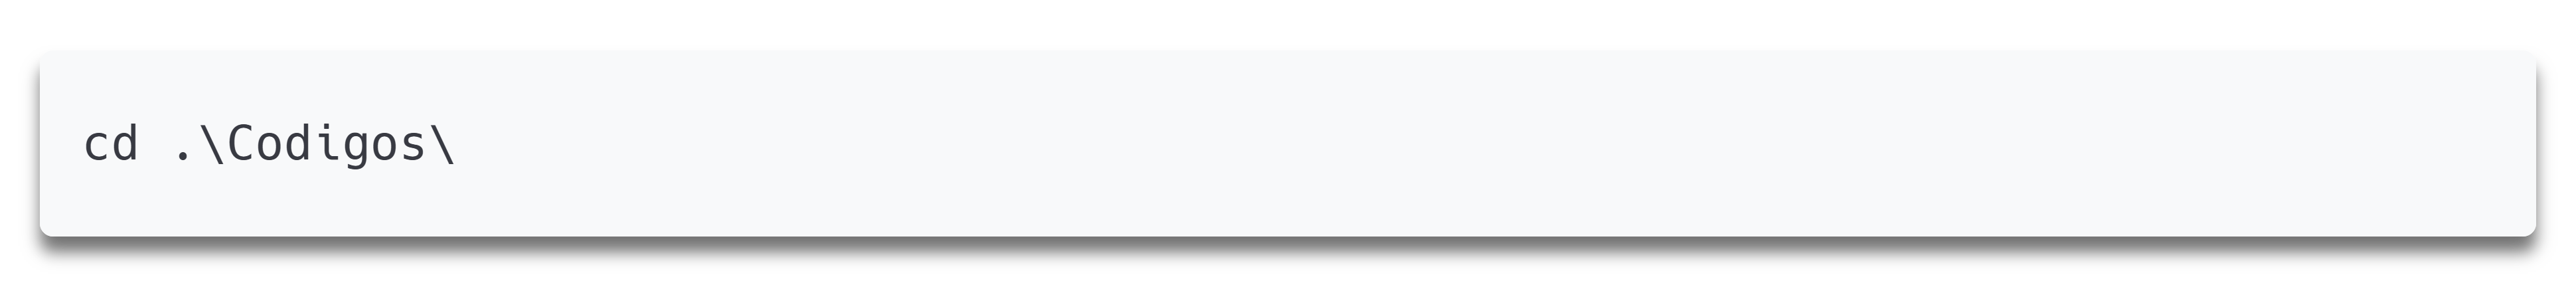
\includegraphics[scale=0.1]{img/mvCodigos.png}
	      \endgroup
	\item Construimos las imagenes utilizando docker compose:
	      \newline
	      \begingroup
	      \centering
	      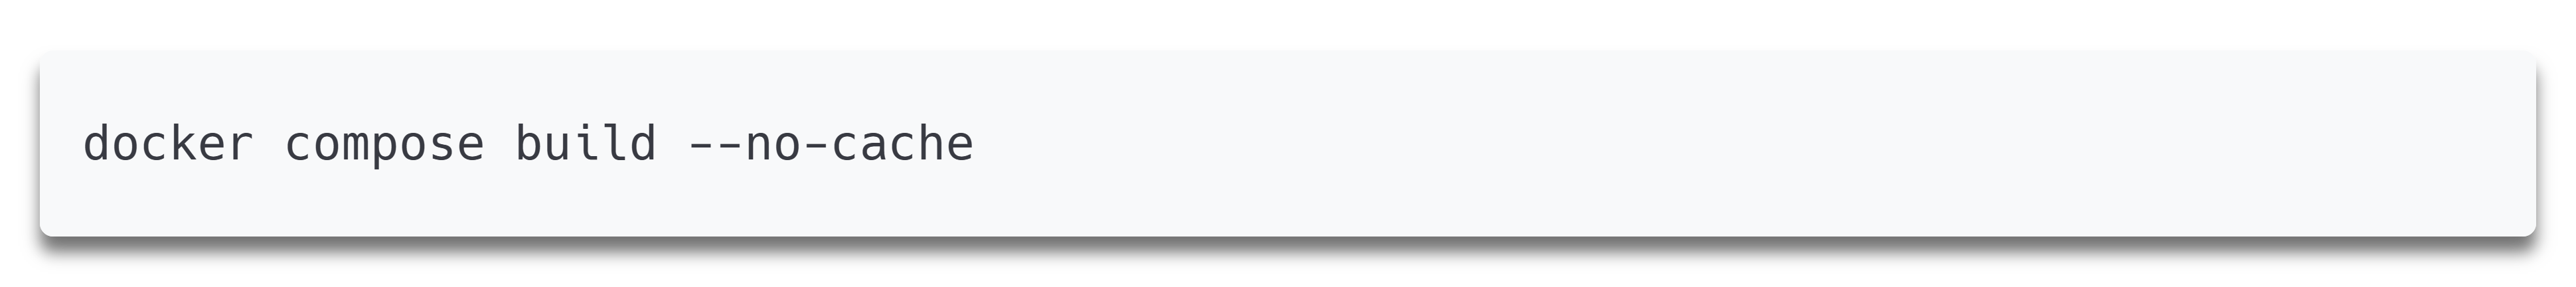
\includegraphics[scale=0.1]{img/dockerBuild.png}
	      \endgroup
	\item Activamos los contenedores:
	      \newline
	      \begingroup
	      \centering
	      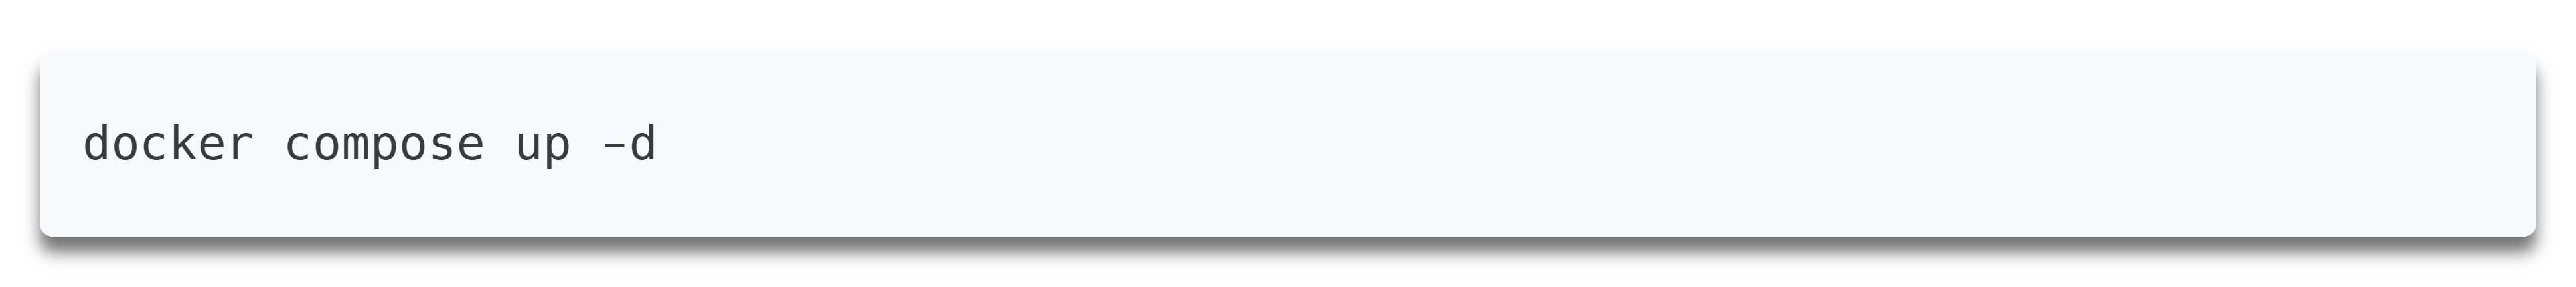
\includegraphics[scale=0.1]{img/dockerUp.png}
	      \endgroup
\end{enumerate}
\subsubsection{Capturas de la interfaz}
\begin{itemize}
	\item \textbf{http://\{IP\}:8000/}
	      \begin{figure}[H]
		      \centering
		      
\includegraphics[scale=0.31]{img/capturaHome.png}
		      \caption{Interfaz del home}
		      \label{fig:interfazHome}
	      \end{figure}

	\item \textbf{http:/\{IP\}:8000/login}
	      \begin{figure}[H]
		      \centering
		      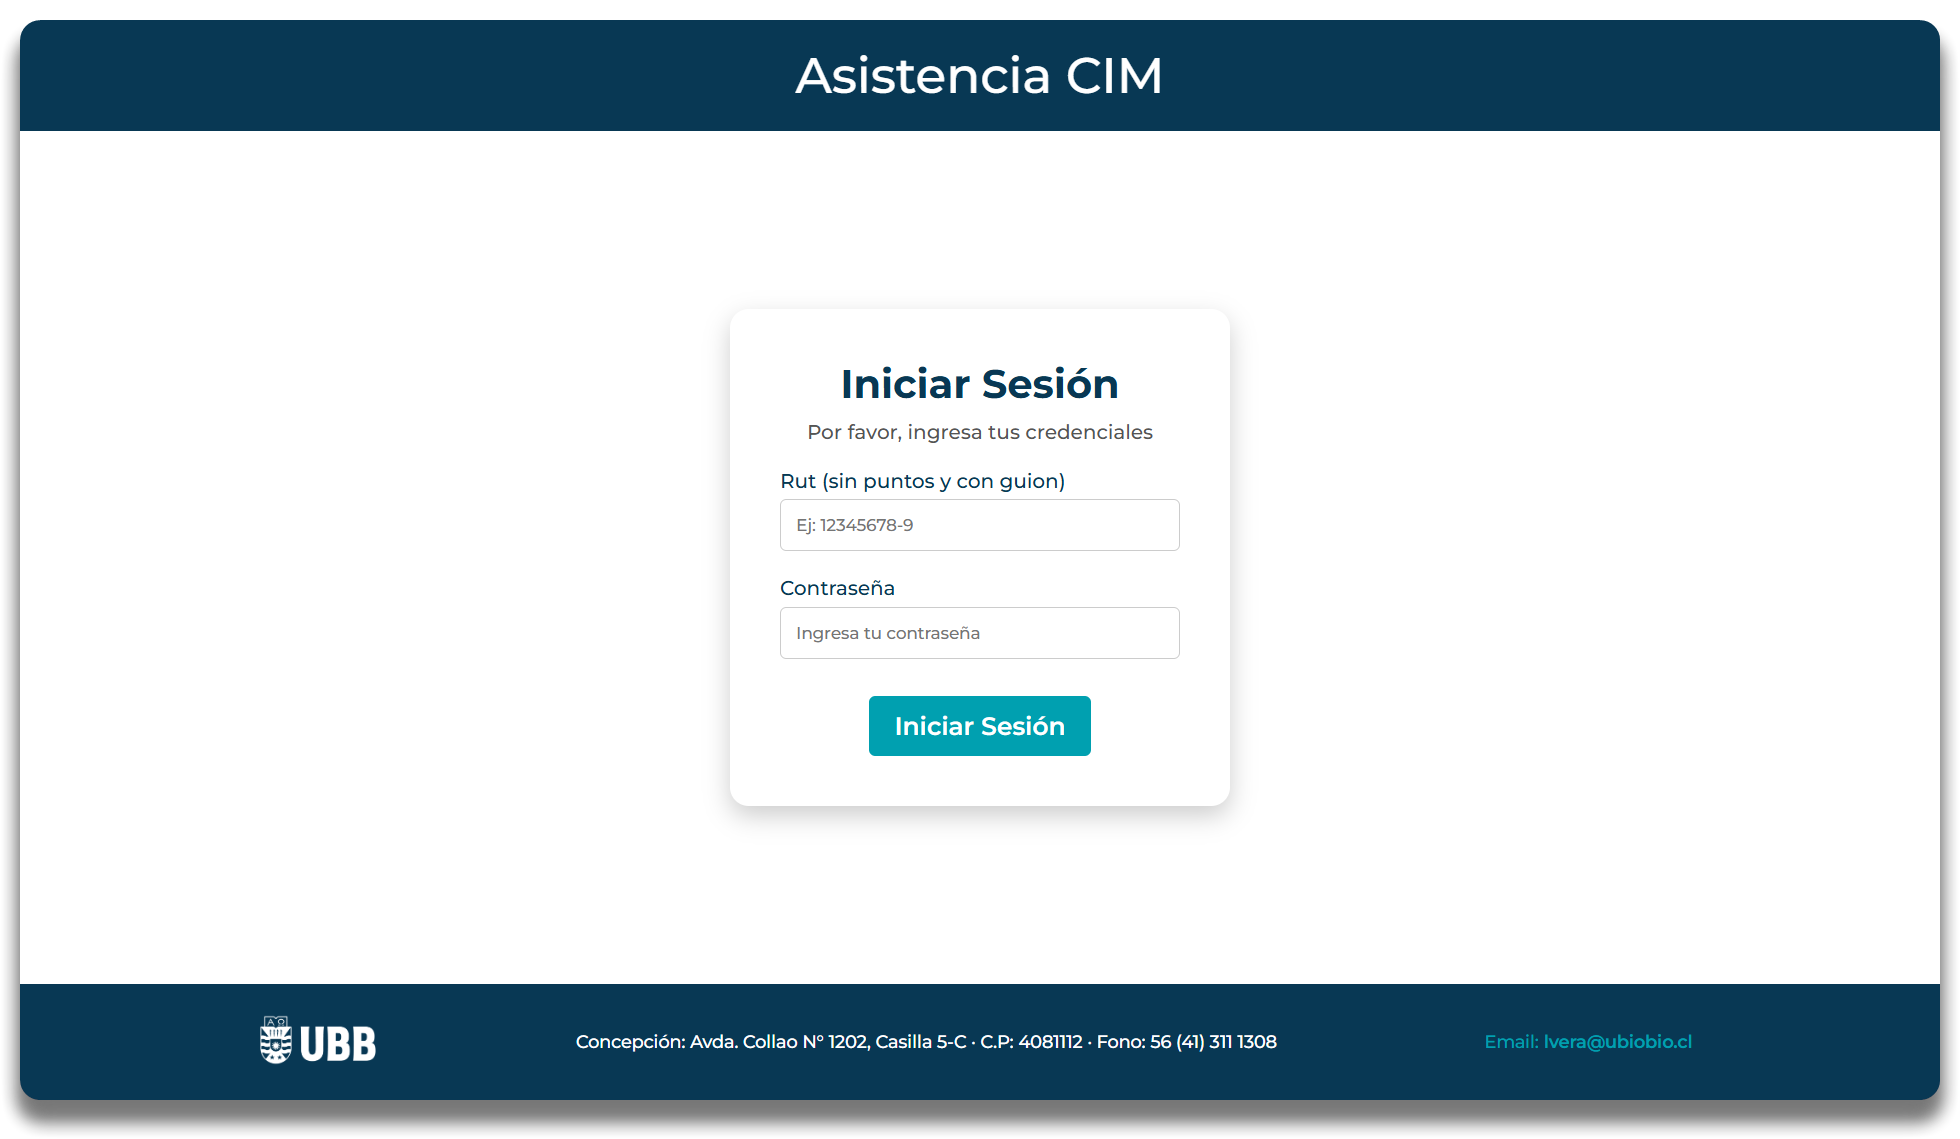
\includegraphics[scale=0.31]{img/capturaLogin.png}
		      \caption{Interfaz del login}
		      \label{fig:interfazLogin}
	      \end{figure}

	\item \textbf{http://\{IP\}:8000/dashboard}
	      \begin{figure}[H]
		      \centering
		      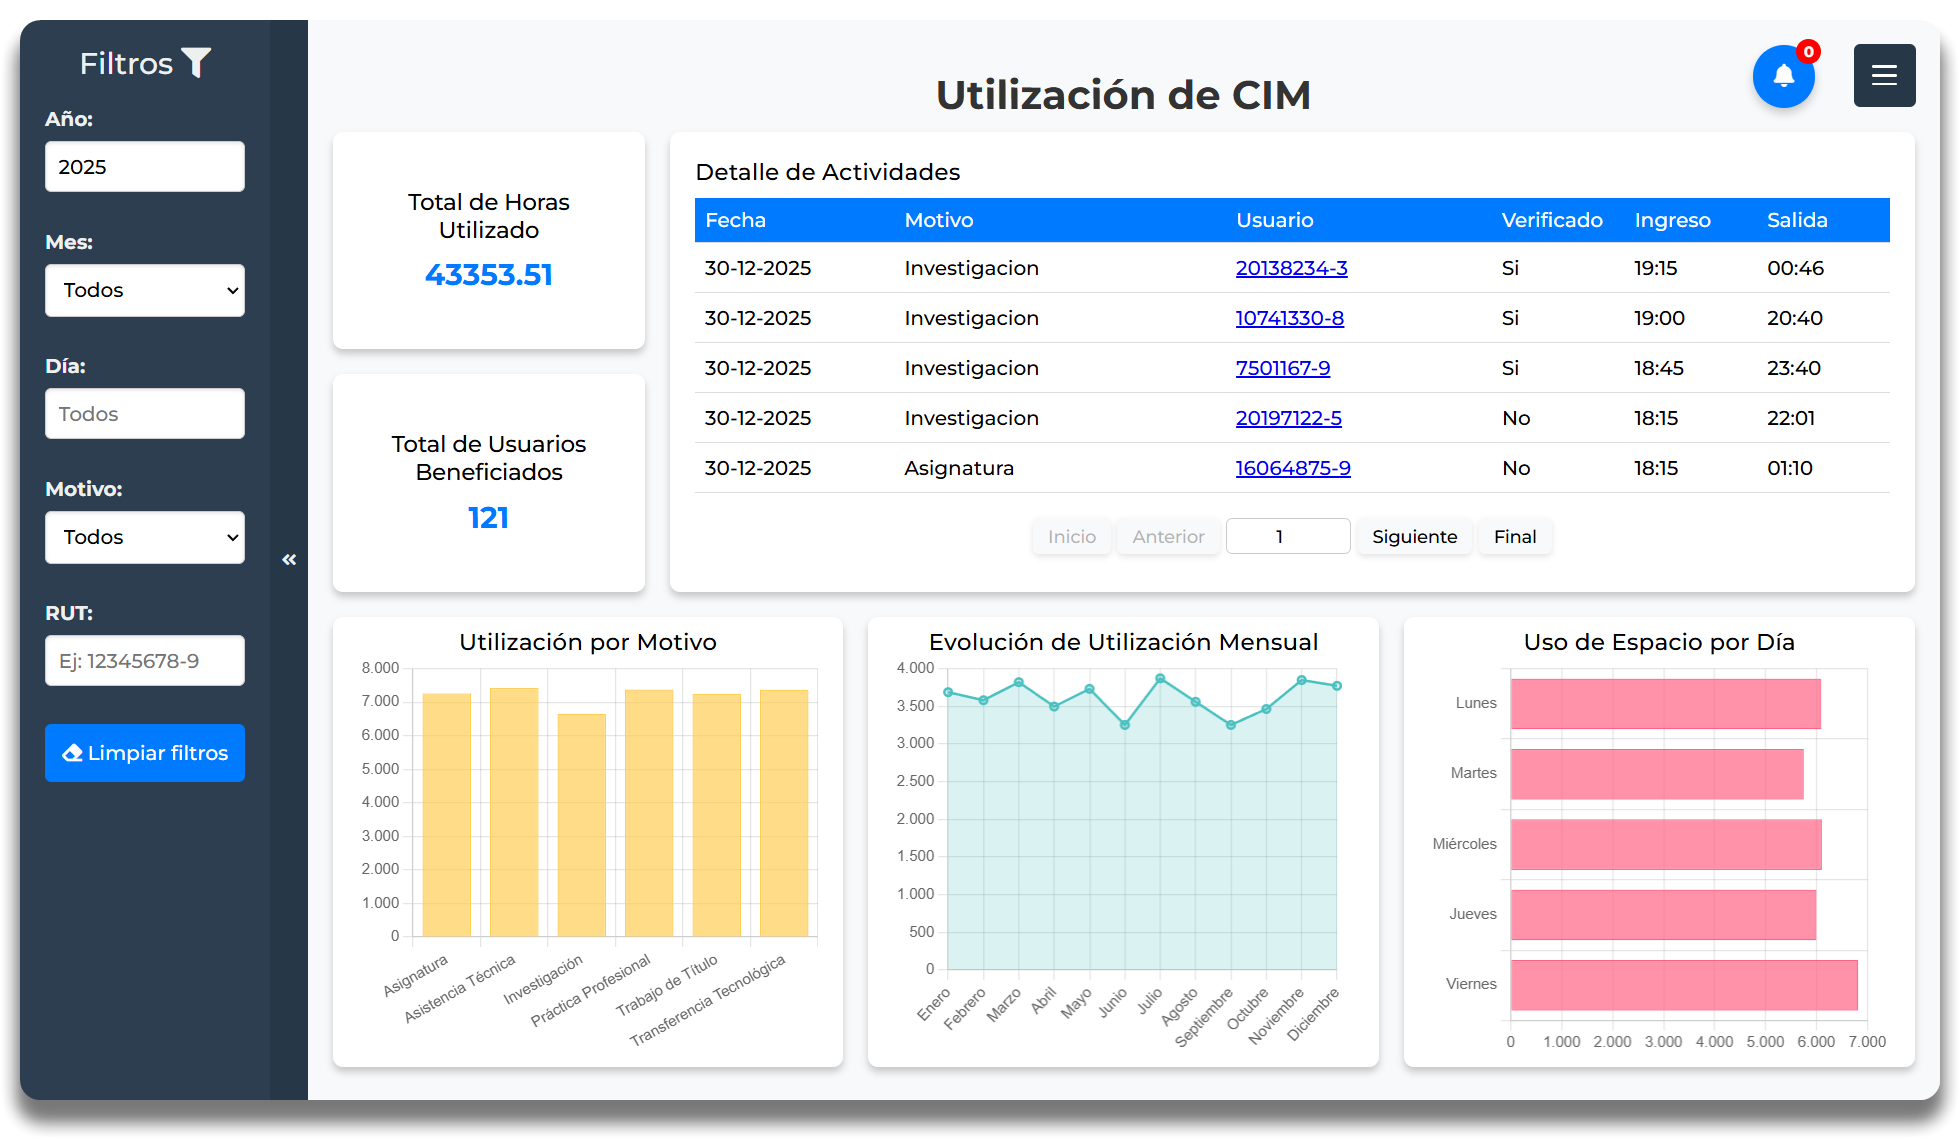
\includegraphics[scale=0.31]{img/capturaDashboard.png}
		      \caption{Interfaz del dashboard}
		      \label{fig:interfazDashboard}
	      \end{figure}
	      \newpage
	\item \textbf{http://\{IP\}:8000/profile?rut=\{RUT\}}
	      \begin{figure}[H]
		      \centering
		      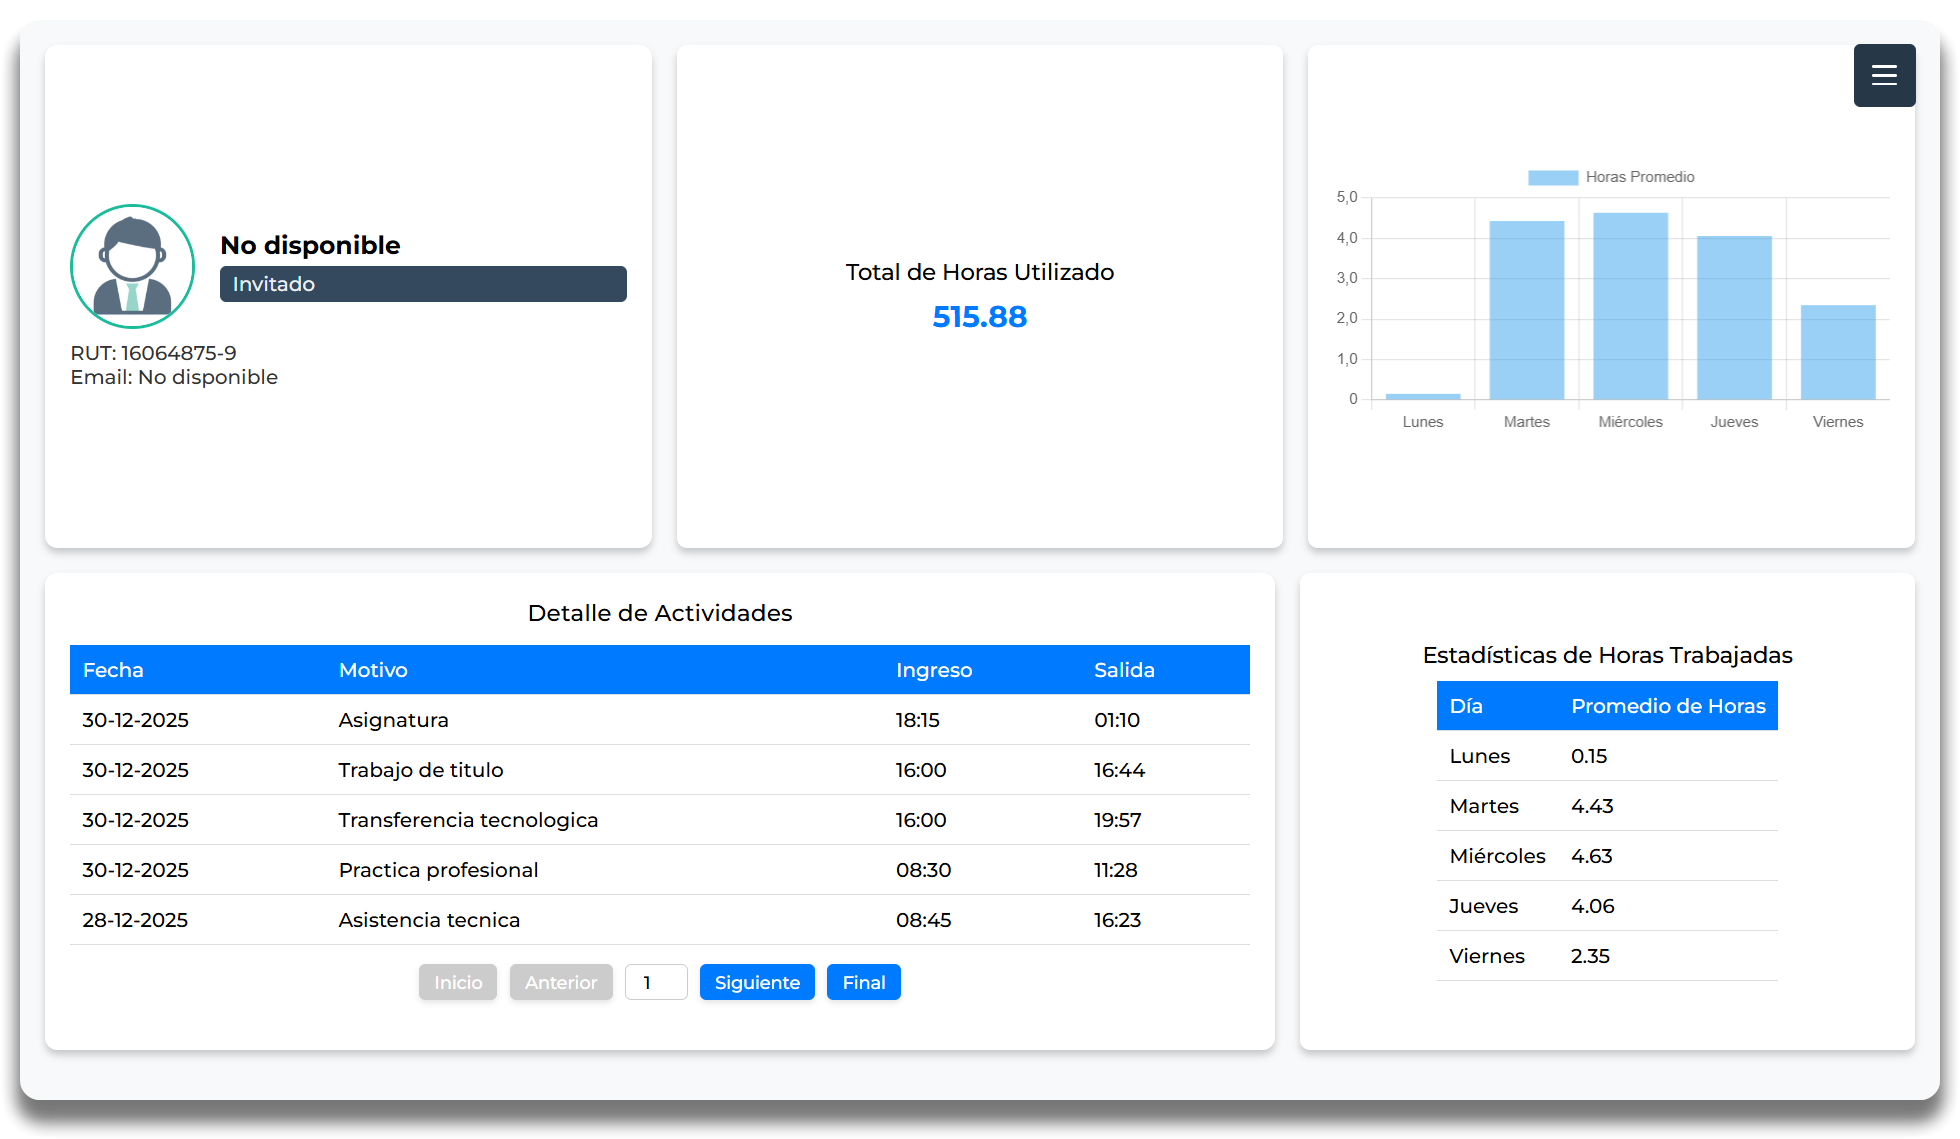
\includegraphics[scale=0.31]{img/capturaProfile.png}
		      \caption{Interfaz del profile}
		      \label{fig:interfazProfile}
	      \end{figure}

	\item \textbf{http://\{IP\}:8000/register-admin}
	      \begin{figure}[H]
		      \centering
		      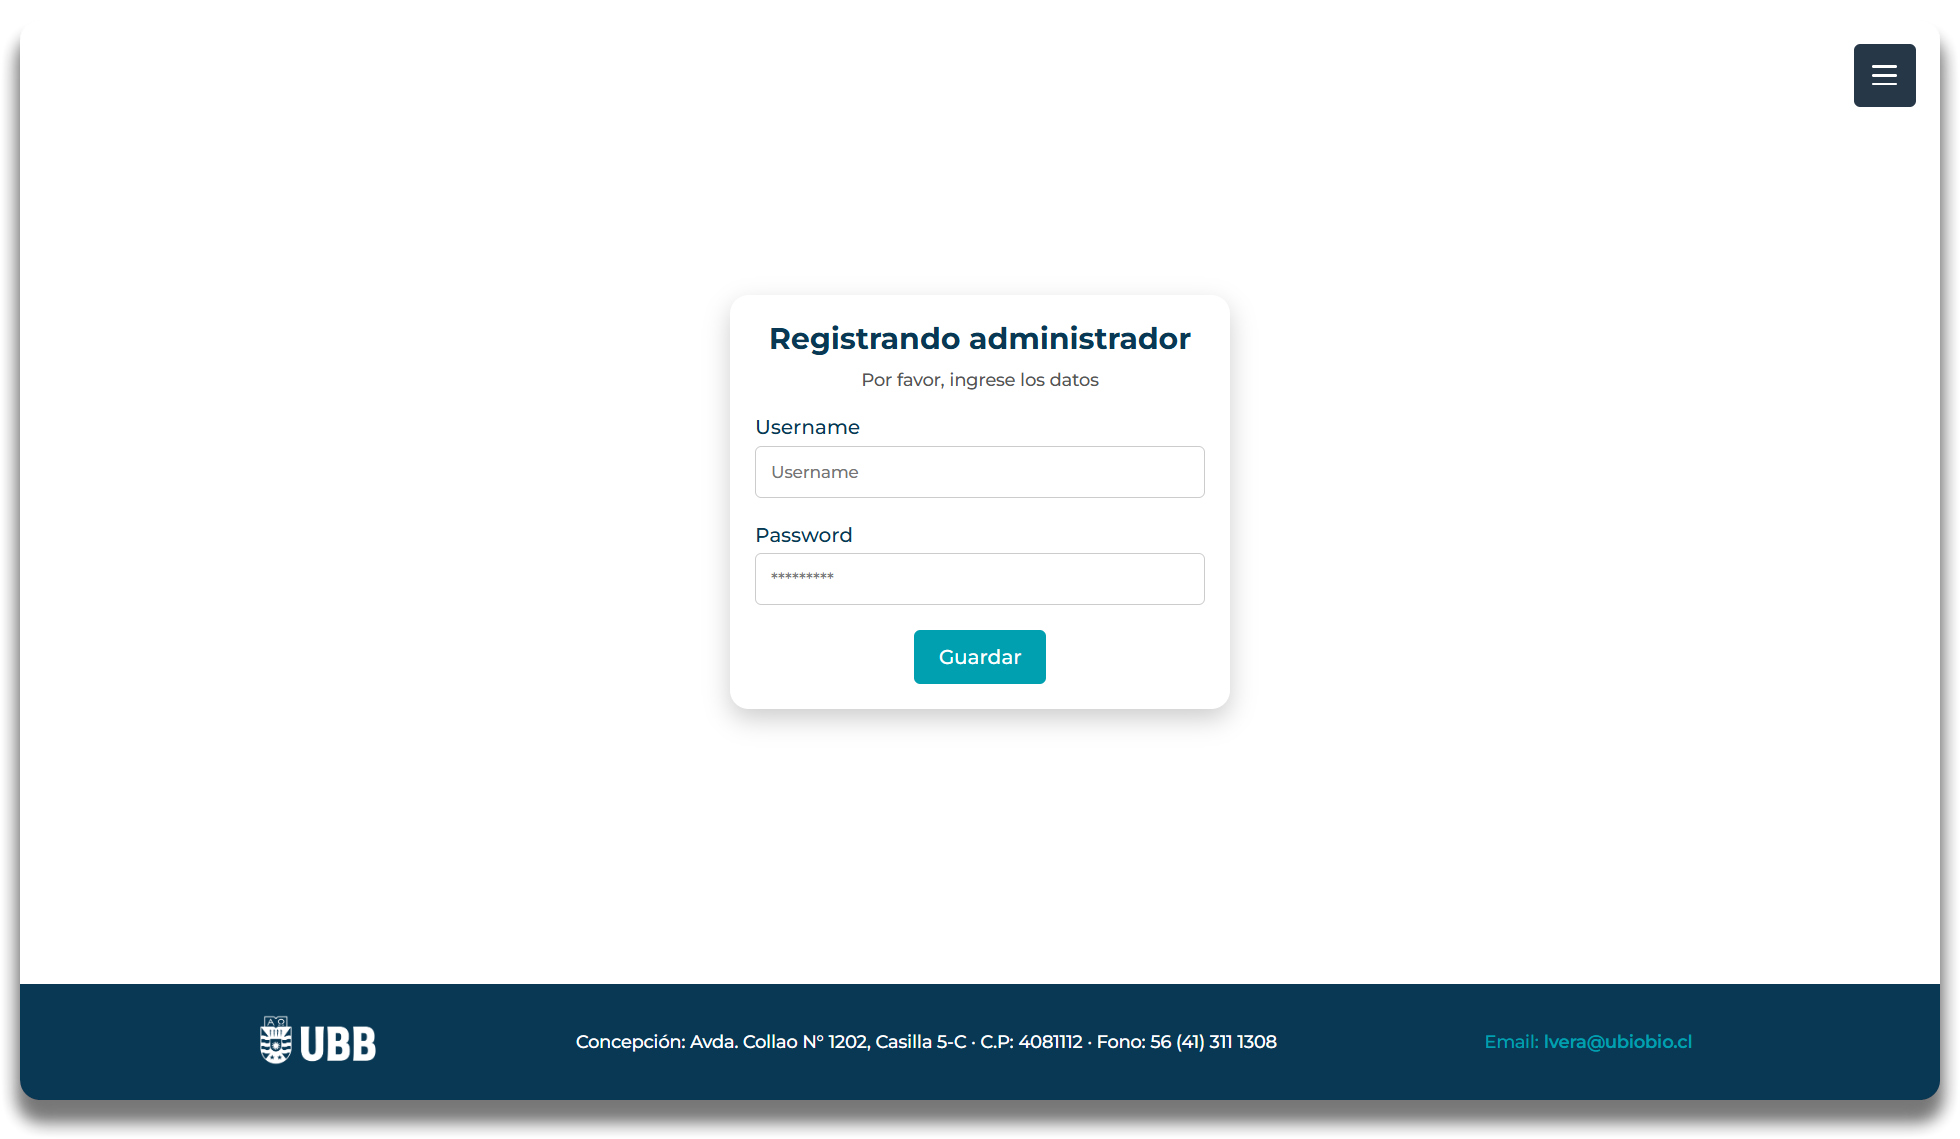
\includegraphics[scale=0.31]{img/capturaRegisterAdmin.png}
		      \caption{Interfaz del register admin}
		      \label{fig:interfazRegisterAdmin}
	      \end{figure}
	      \newpage
	\item \textbf{http://\{IP\}:8000/register-user}
	      \begin{figure}[H]
		      \centering
		      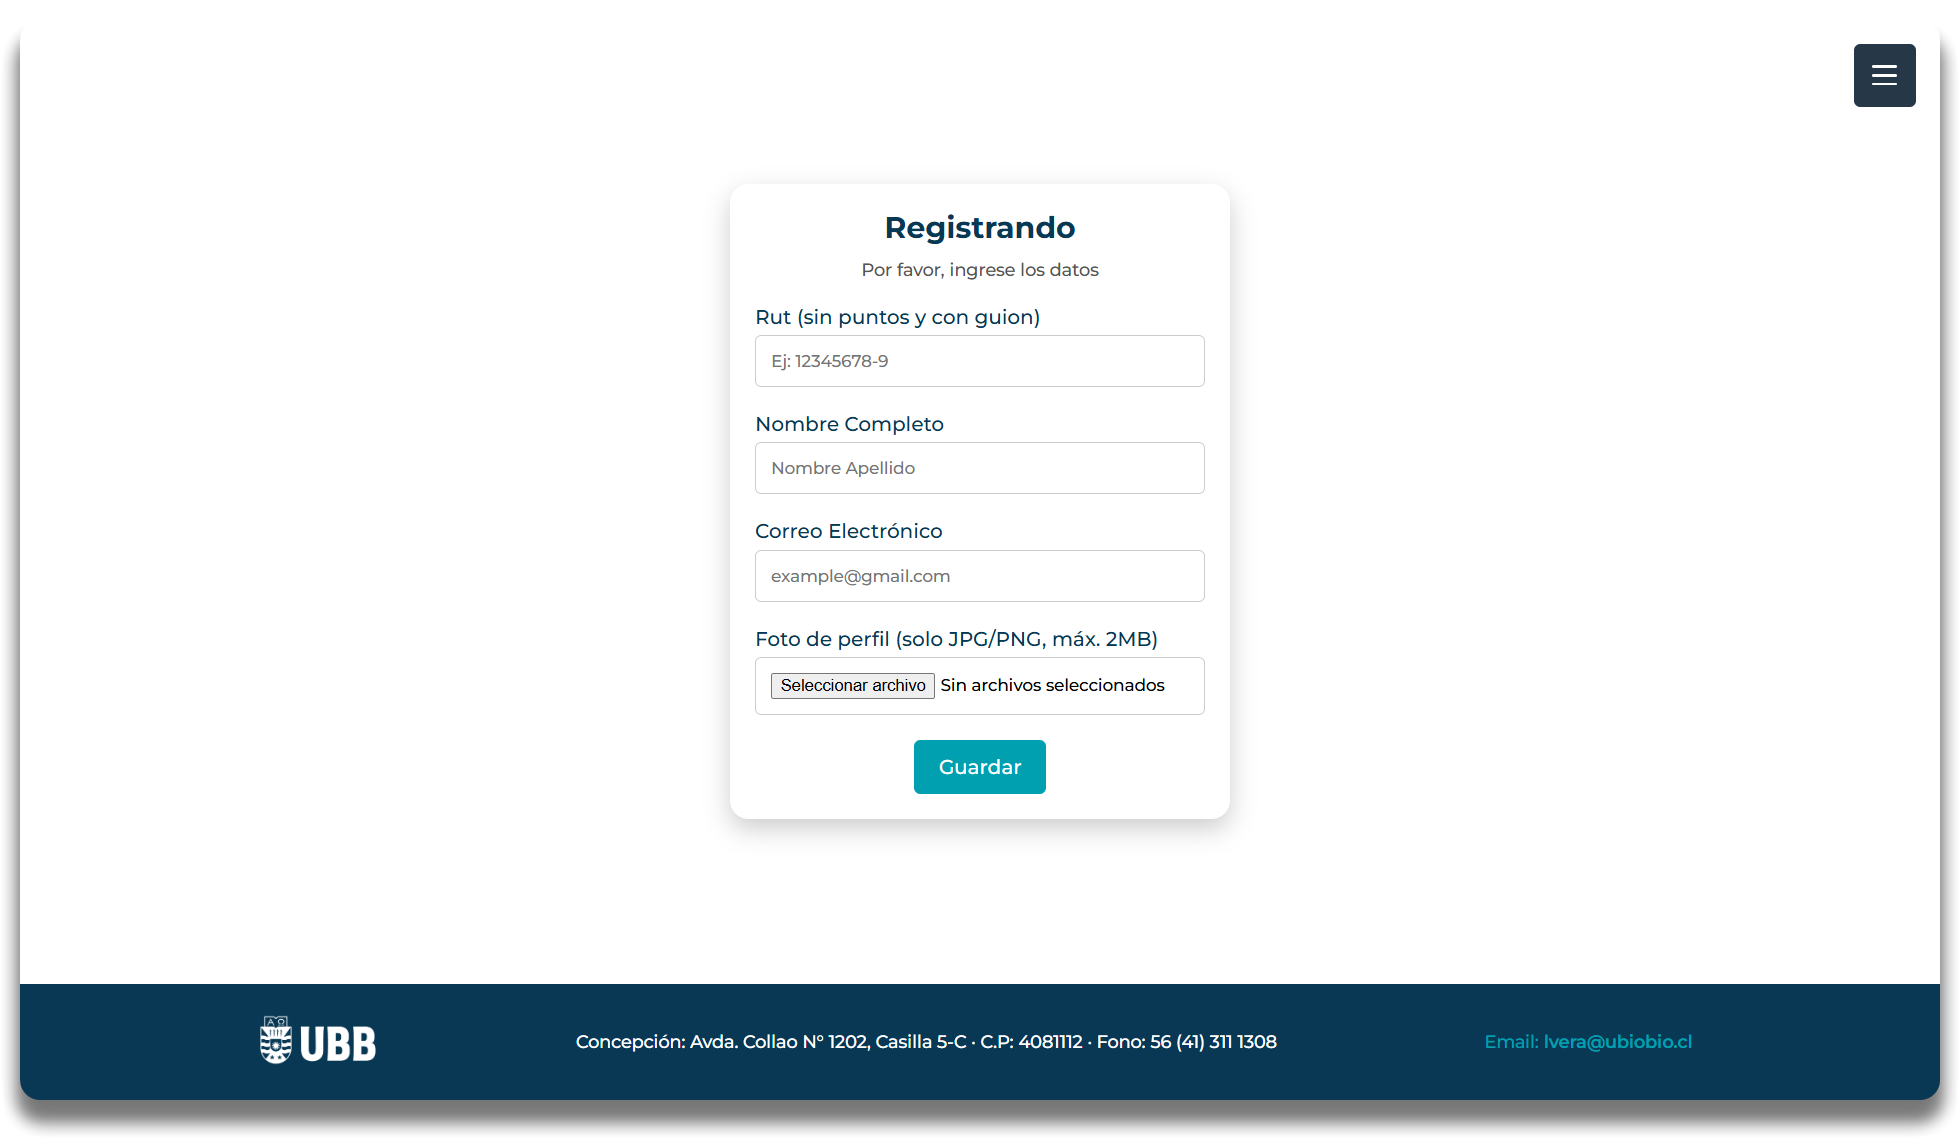
\includegraphics[scale=0.31]{img/capturaRegisterUser.png}
		      \caption{Interfaz del register user}
		      \label{fig:interfazRegisterUser}
	      \end{figure}

	\item Componentes Navbar y Notify:
	      \newline
	      \begin{minipage}{0.45\textwidth}
		      \centering
		      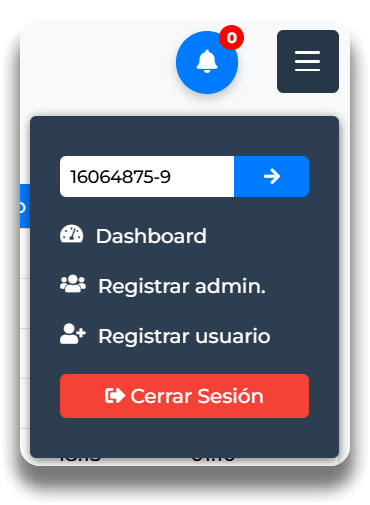
\includegraphics[height=8cm]{img/capturaNavbar.png}
		      \captionof{figure}{Componente Navbar}
		      \label{fig:componenteNavbar}
	      \end{minipage}
	      \hfill
	      \begin{minipage}{0.45\textwidth}
		      \centering
		      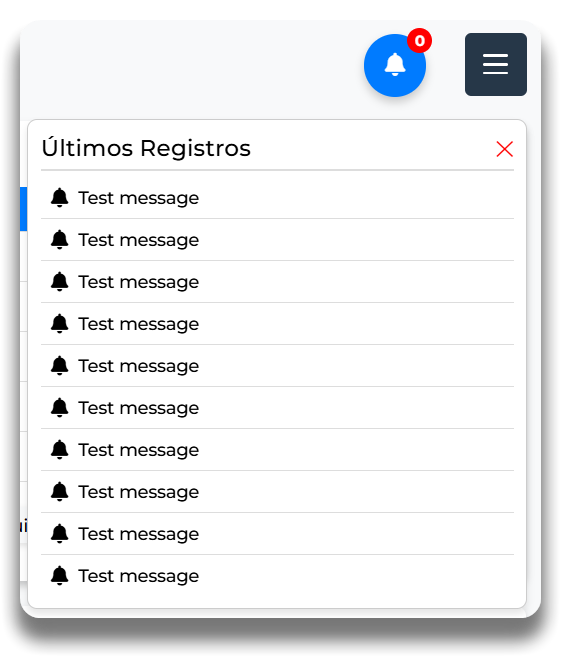
\includegraphics[height=8cm]{img/capturaNotify.png}
		      \captionof{figure}{Componente Notify}
		      \label{fig:componenteNotify}
	      \end{minipage}


\end{itemize}
\newpage
\subsubsection{Código}
Por la obvia cantidad de código que engloba todo el proyecto se dejara captura de gran parte del código y se explicara algunas de las partes que al autor le parecen importantes.
\begin{enumerate}
	\item \textbf{auth.py}:
	      \begin{enumerate}
		      \item La importación de librerías, la obtención del secreto y la duración del token:
		            \begin{figure}[H]
			            \centering
			            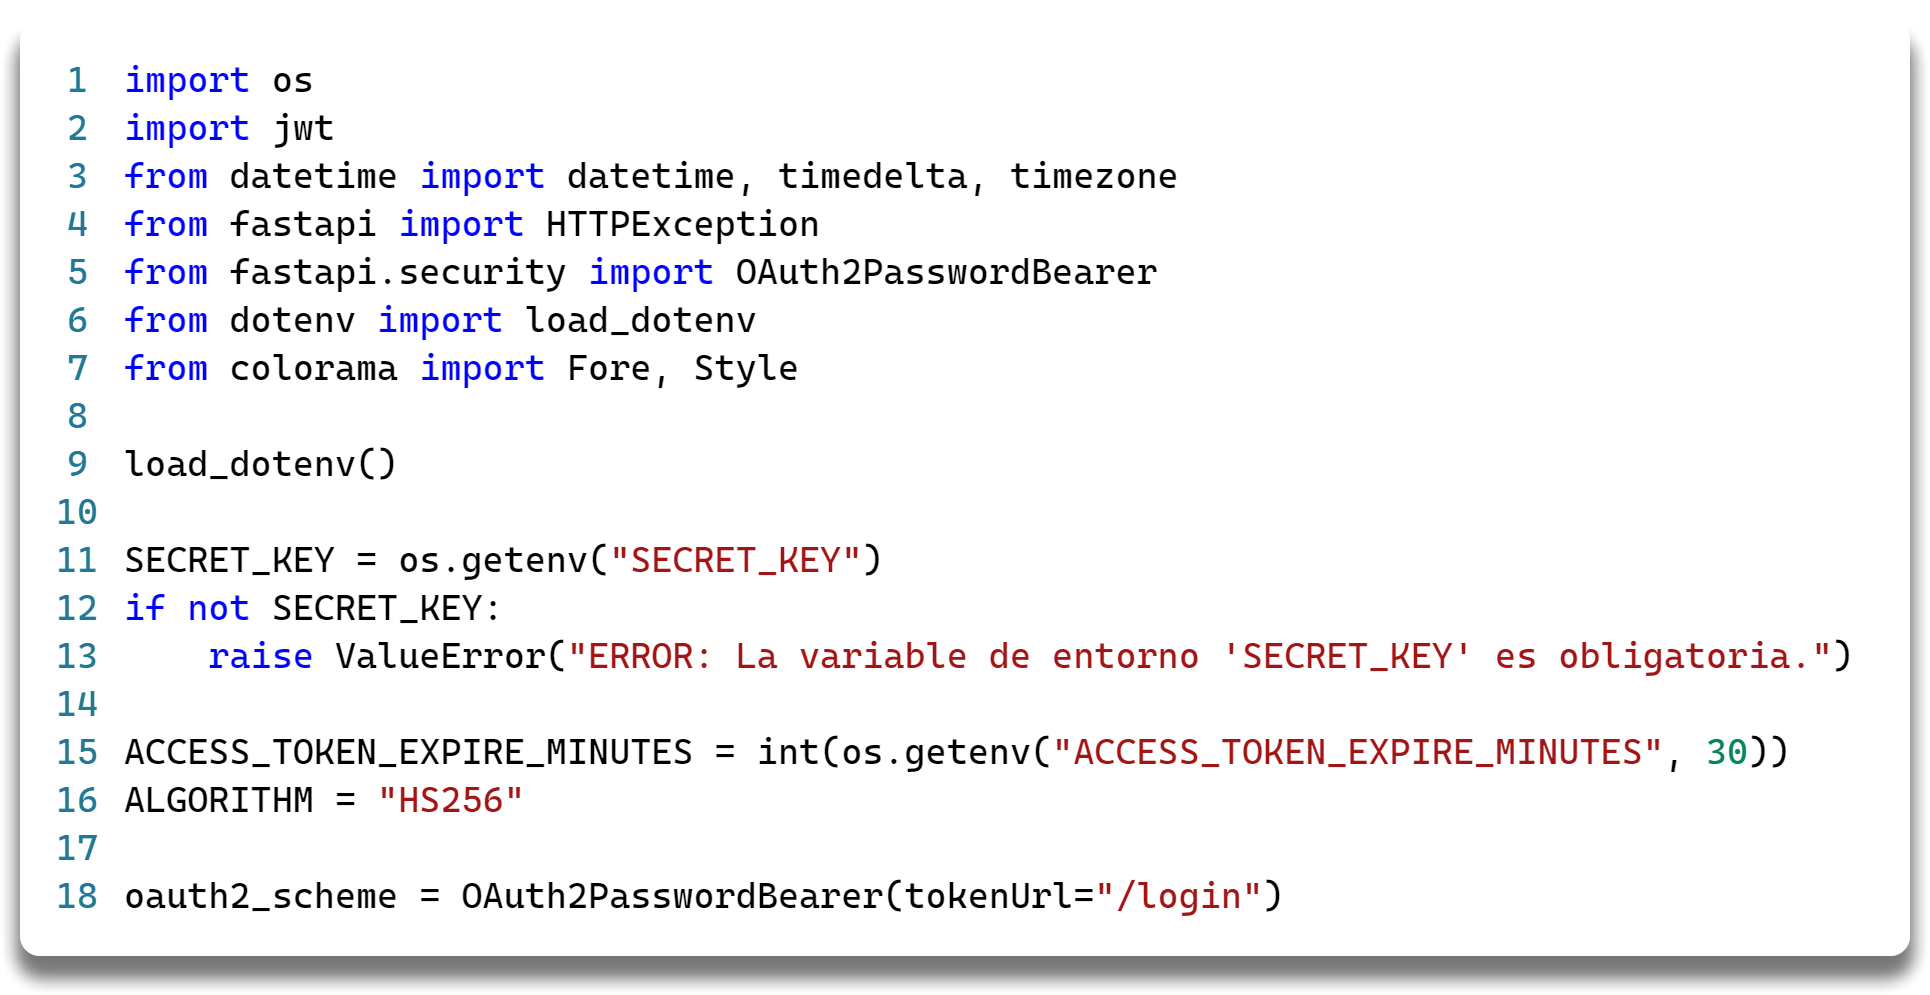
\includegraphics[width=\textwidth]{img/auth1.png}
			            \caption{Archivo auth.py Parte I}
			            \label{fig:auth1}
		            \end{figure}
		      \item Una función que crea un token JWT para el login del supervisor:
		            \begin{figure}[H]
			            \centering
			            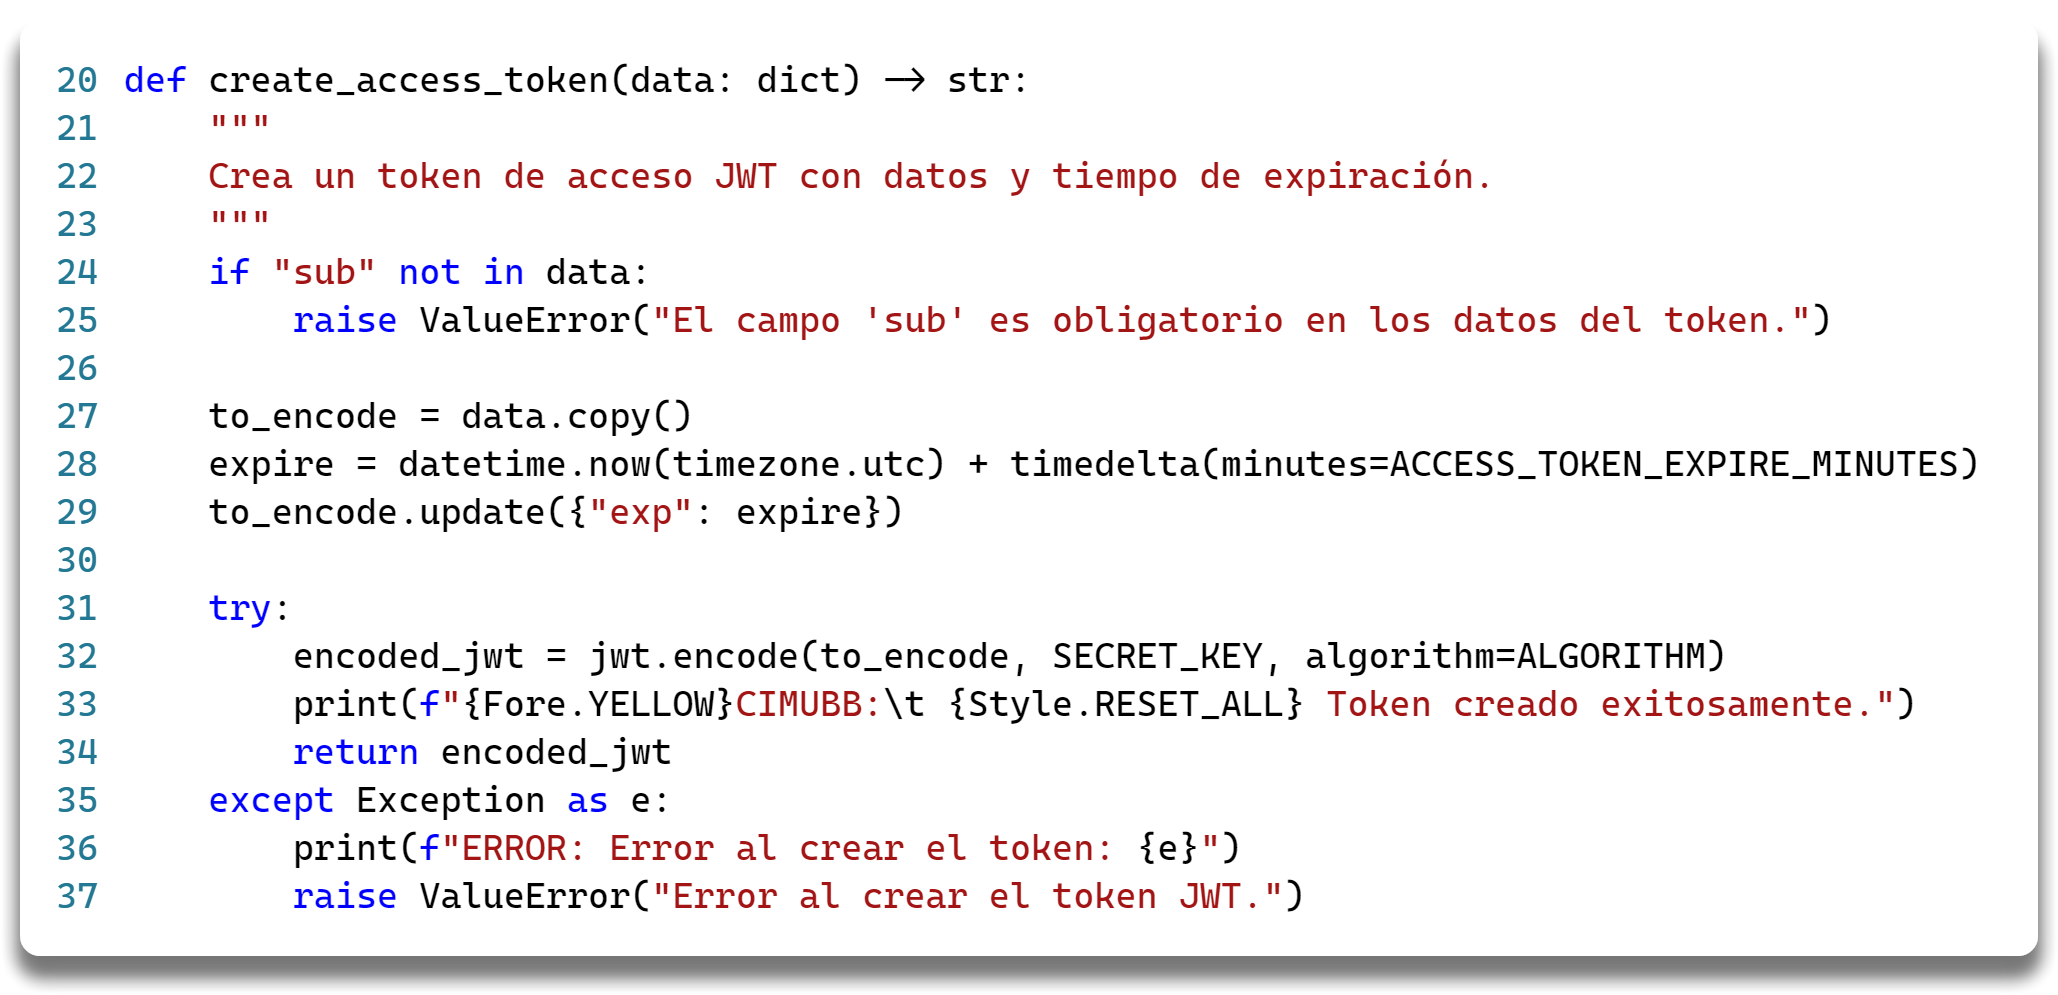
\includegraphics[width=\textwidth]{img/auth2.png}
			            \caption{Archivo auth.py Parte II}
			            \label{fig:auth2}
		            \end{figure}
		      \item Una función que verifica si el token es inválido o a sido experida al pasar los 30 minutos:
		            \begin{figure}[H]
			            \centering
			            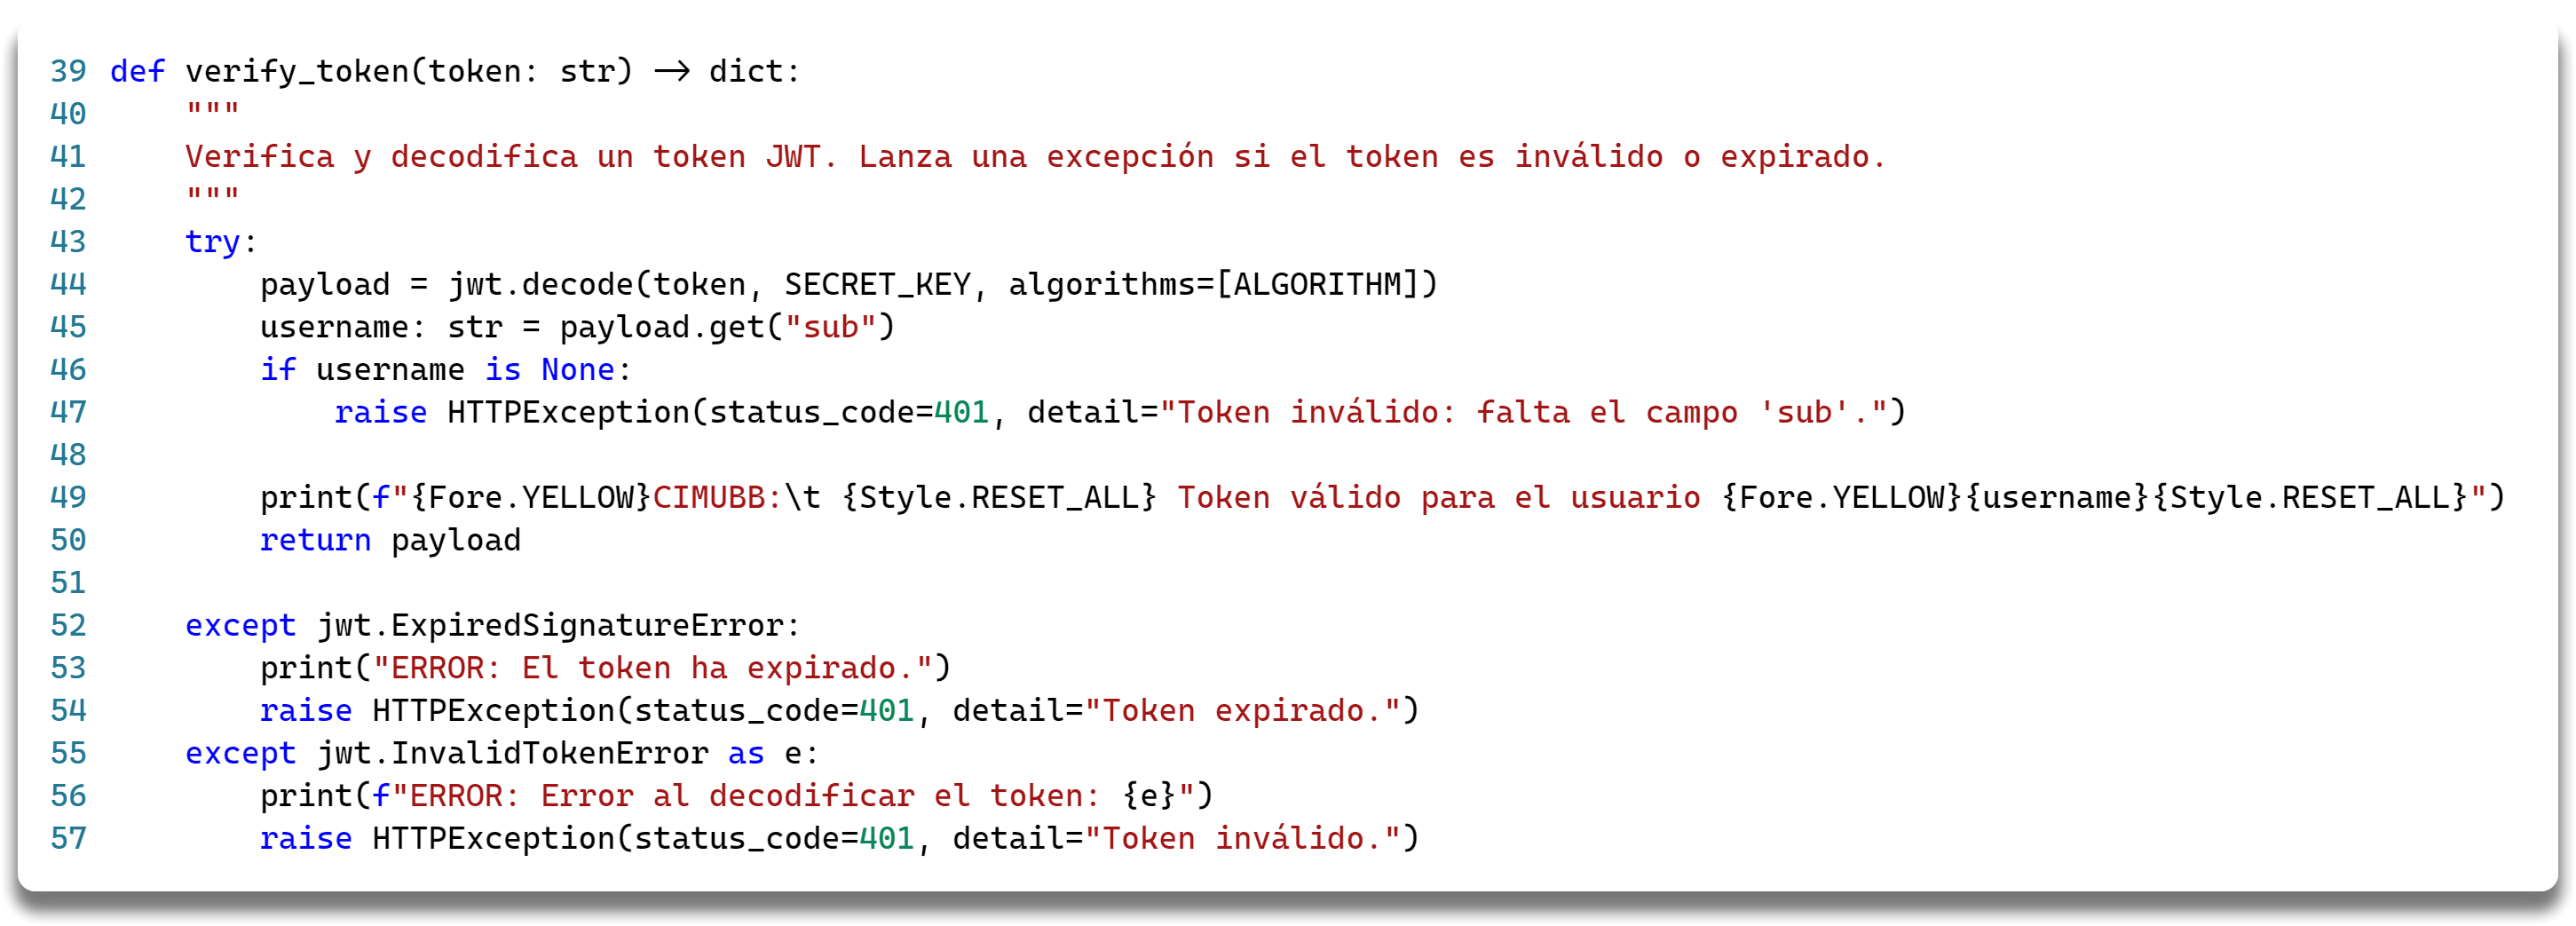
\includegraphics[width=\textwidth]{img/auth3.png}
			            \caption{Archivo auth.py Parte III}
			            \label{fig:auth3}
		            \end{figure}
	      \end{enumerate}

	\item \textbf{security.py}:
	      \begin{enumerate}
		      \item Se crean 2 funciones que permiten comparar el hash del password del login:
		            \begin{figure}[H]
			            \centering
			            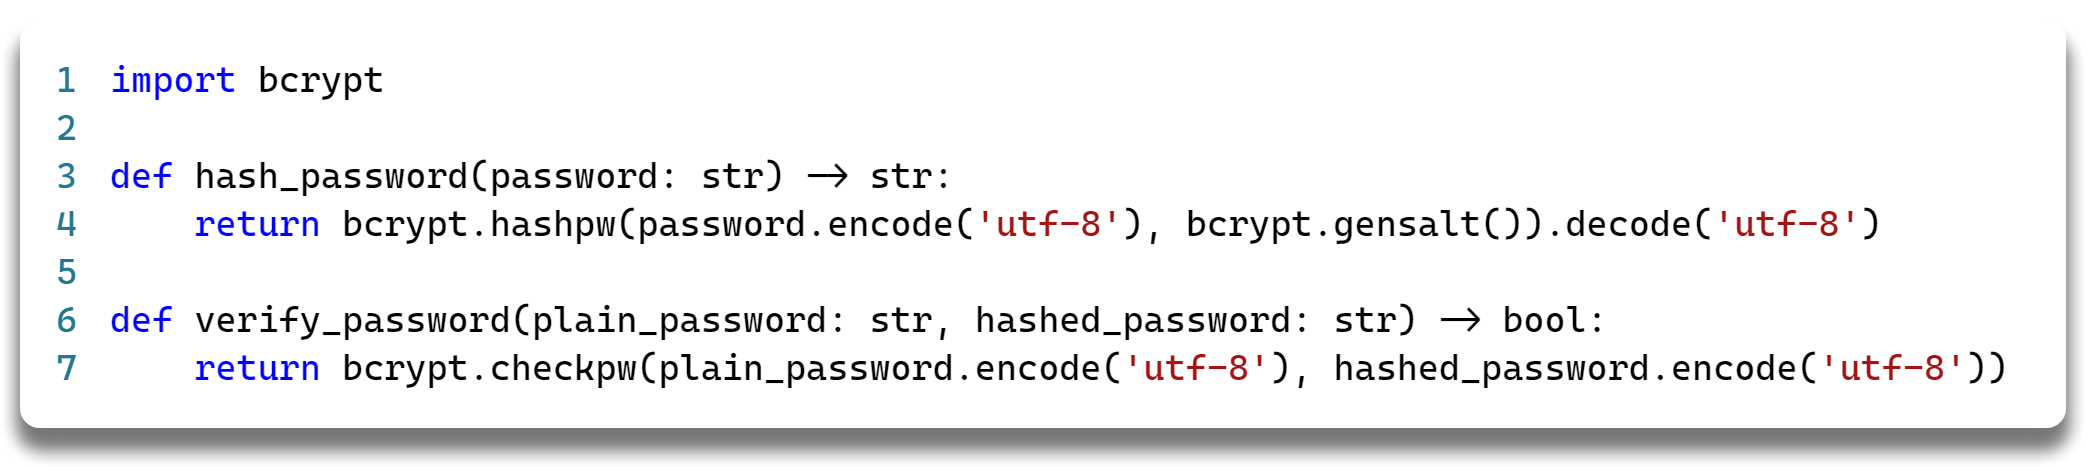
\includegraphics[width=\textwidth]{img/security.png}
			            \caption{Archivo security.py}
			            \label{fig:security}
		            \end{figure}
	      \end{enumerate}
	      \newpage
	\item \textbf{database.py}:
	      \begin{enumerate}
		      \item Importación de librerías, creación de objeto Database y conexión por piscinas, lo que mejora significativamente la cantidad simultánea de consultas:
		            \begin{figure}[H]
			            \centering
			            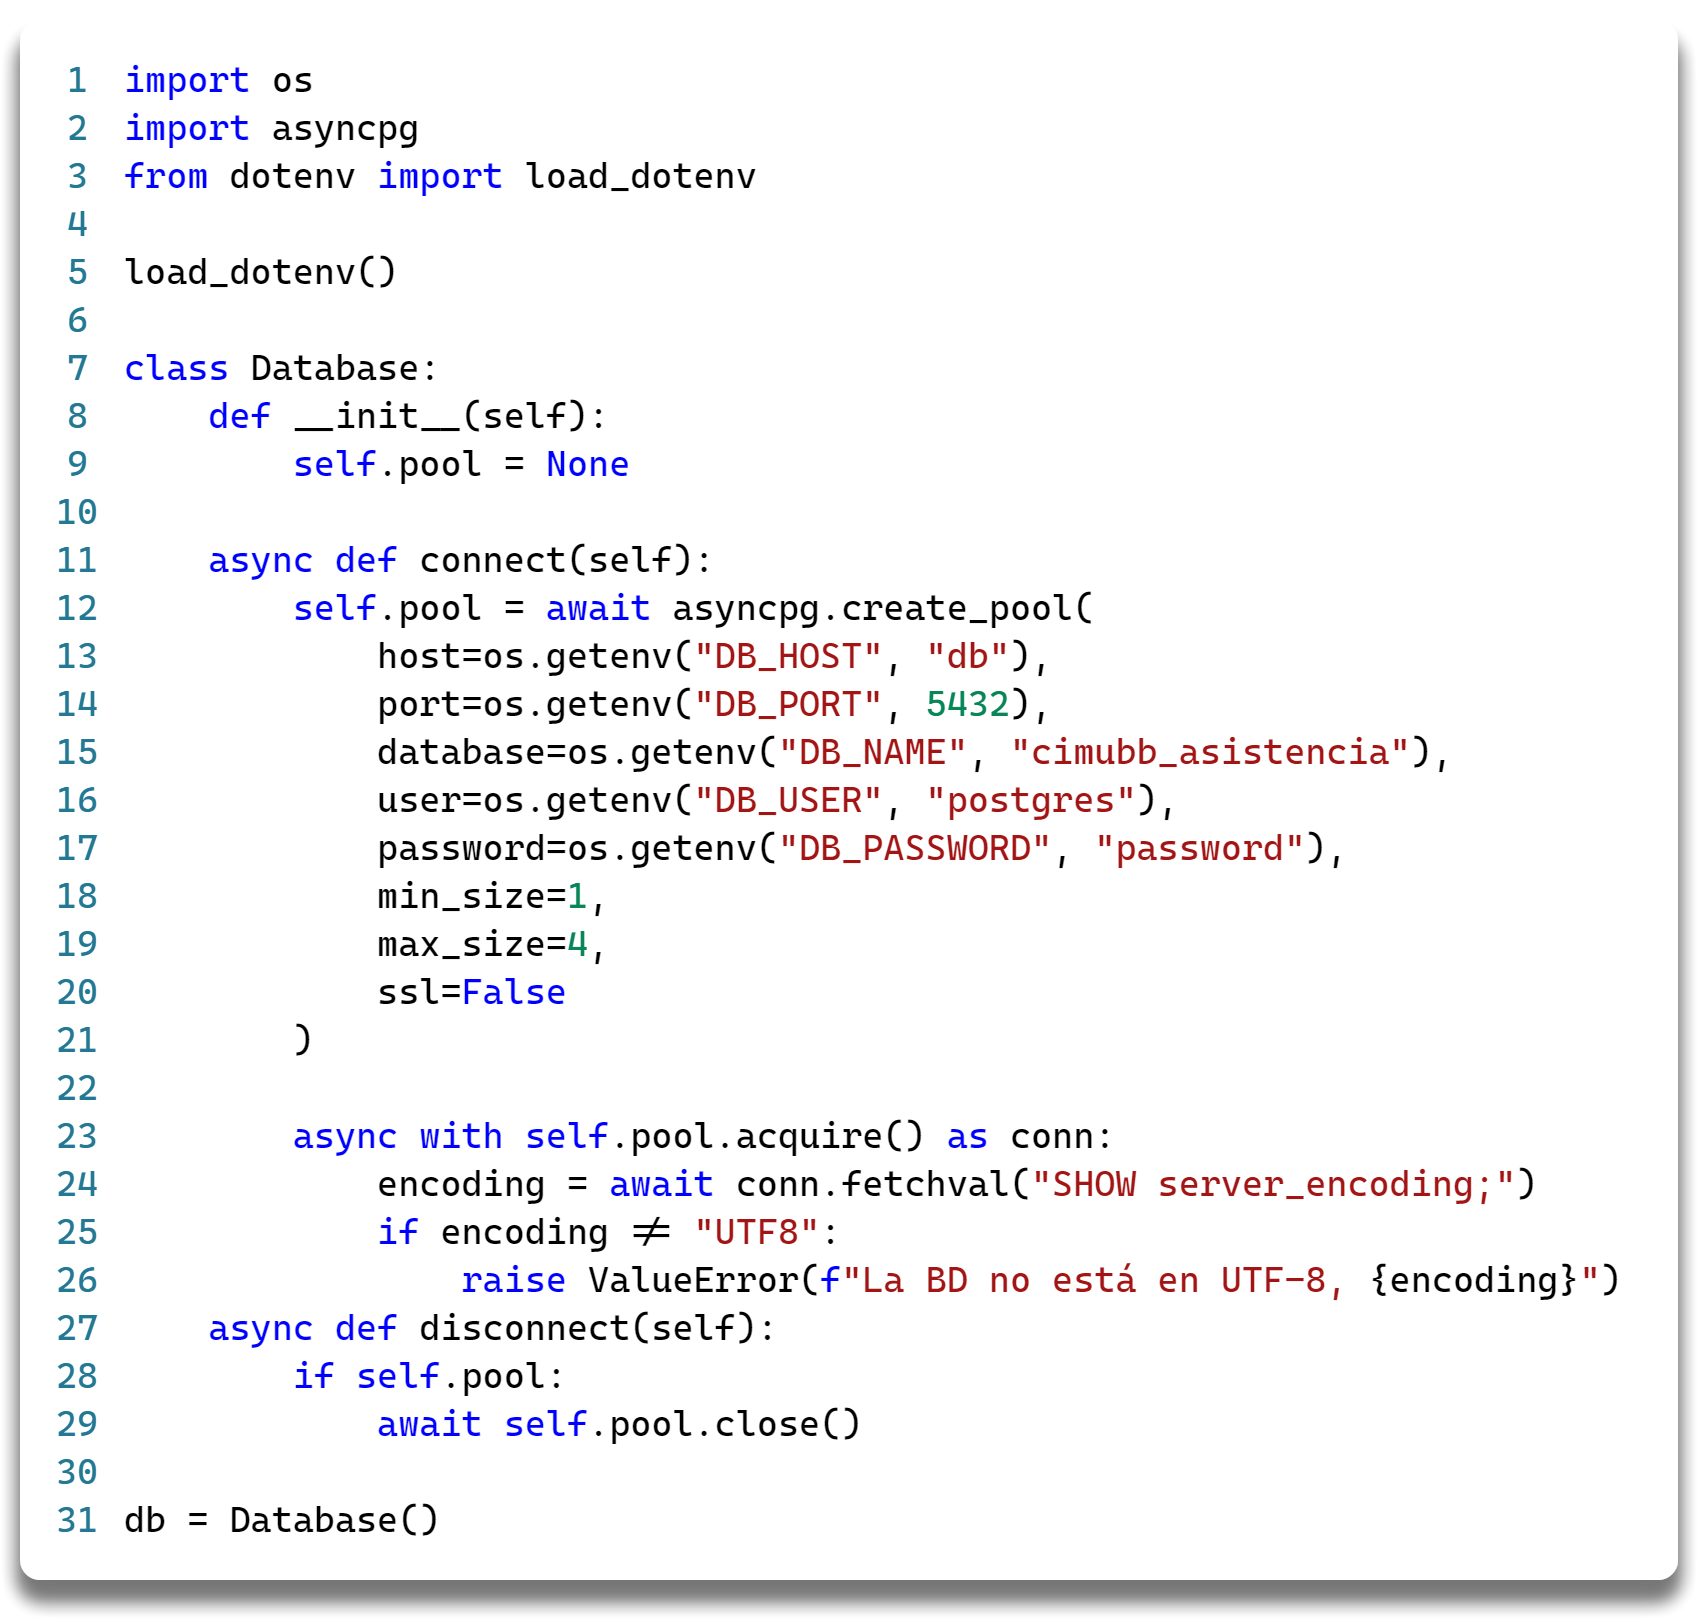
\includegraphics[width=0.9\textwidth]{img/database.png}
			            \caption{Archivo database.py}
			            \label{fig:database}
		            \end{figure}
	      \end{enumerate}

	\item \textbf{query.py}:
	      \begin{enumerate}
		      \item Importación de librerías:
		            \begin{figure}[H]
			            \centering
			            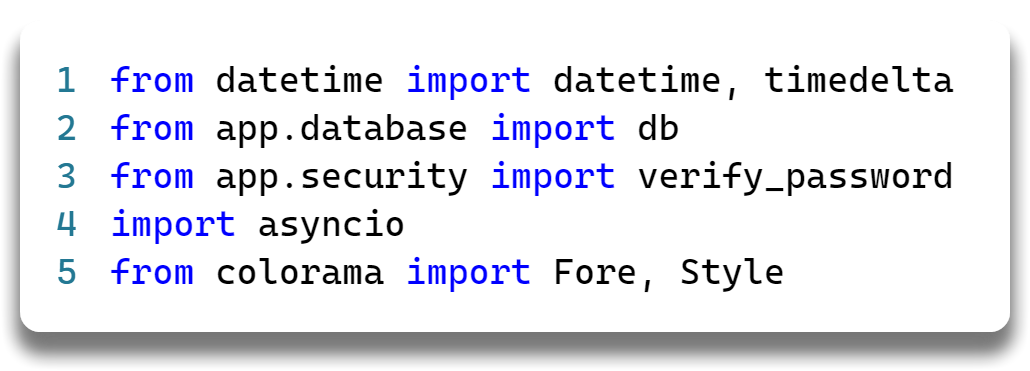
\includegraphics[width=0.6\textwidth]{img/query1.png}
			            \caption{Archivo query.py Parte I}
			            \label{fig:query1}
		            \end{figure}
		      \item Función principal que obtiene todos los datos a mostrar en el dashboard según los parametros:
		            \begin{figure}[H]
			            \centering
			            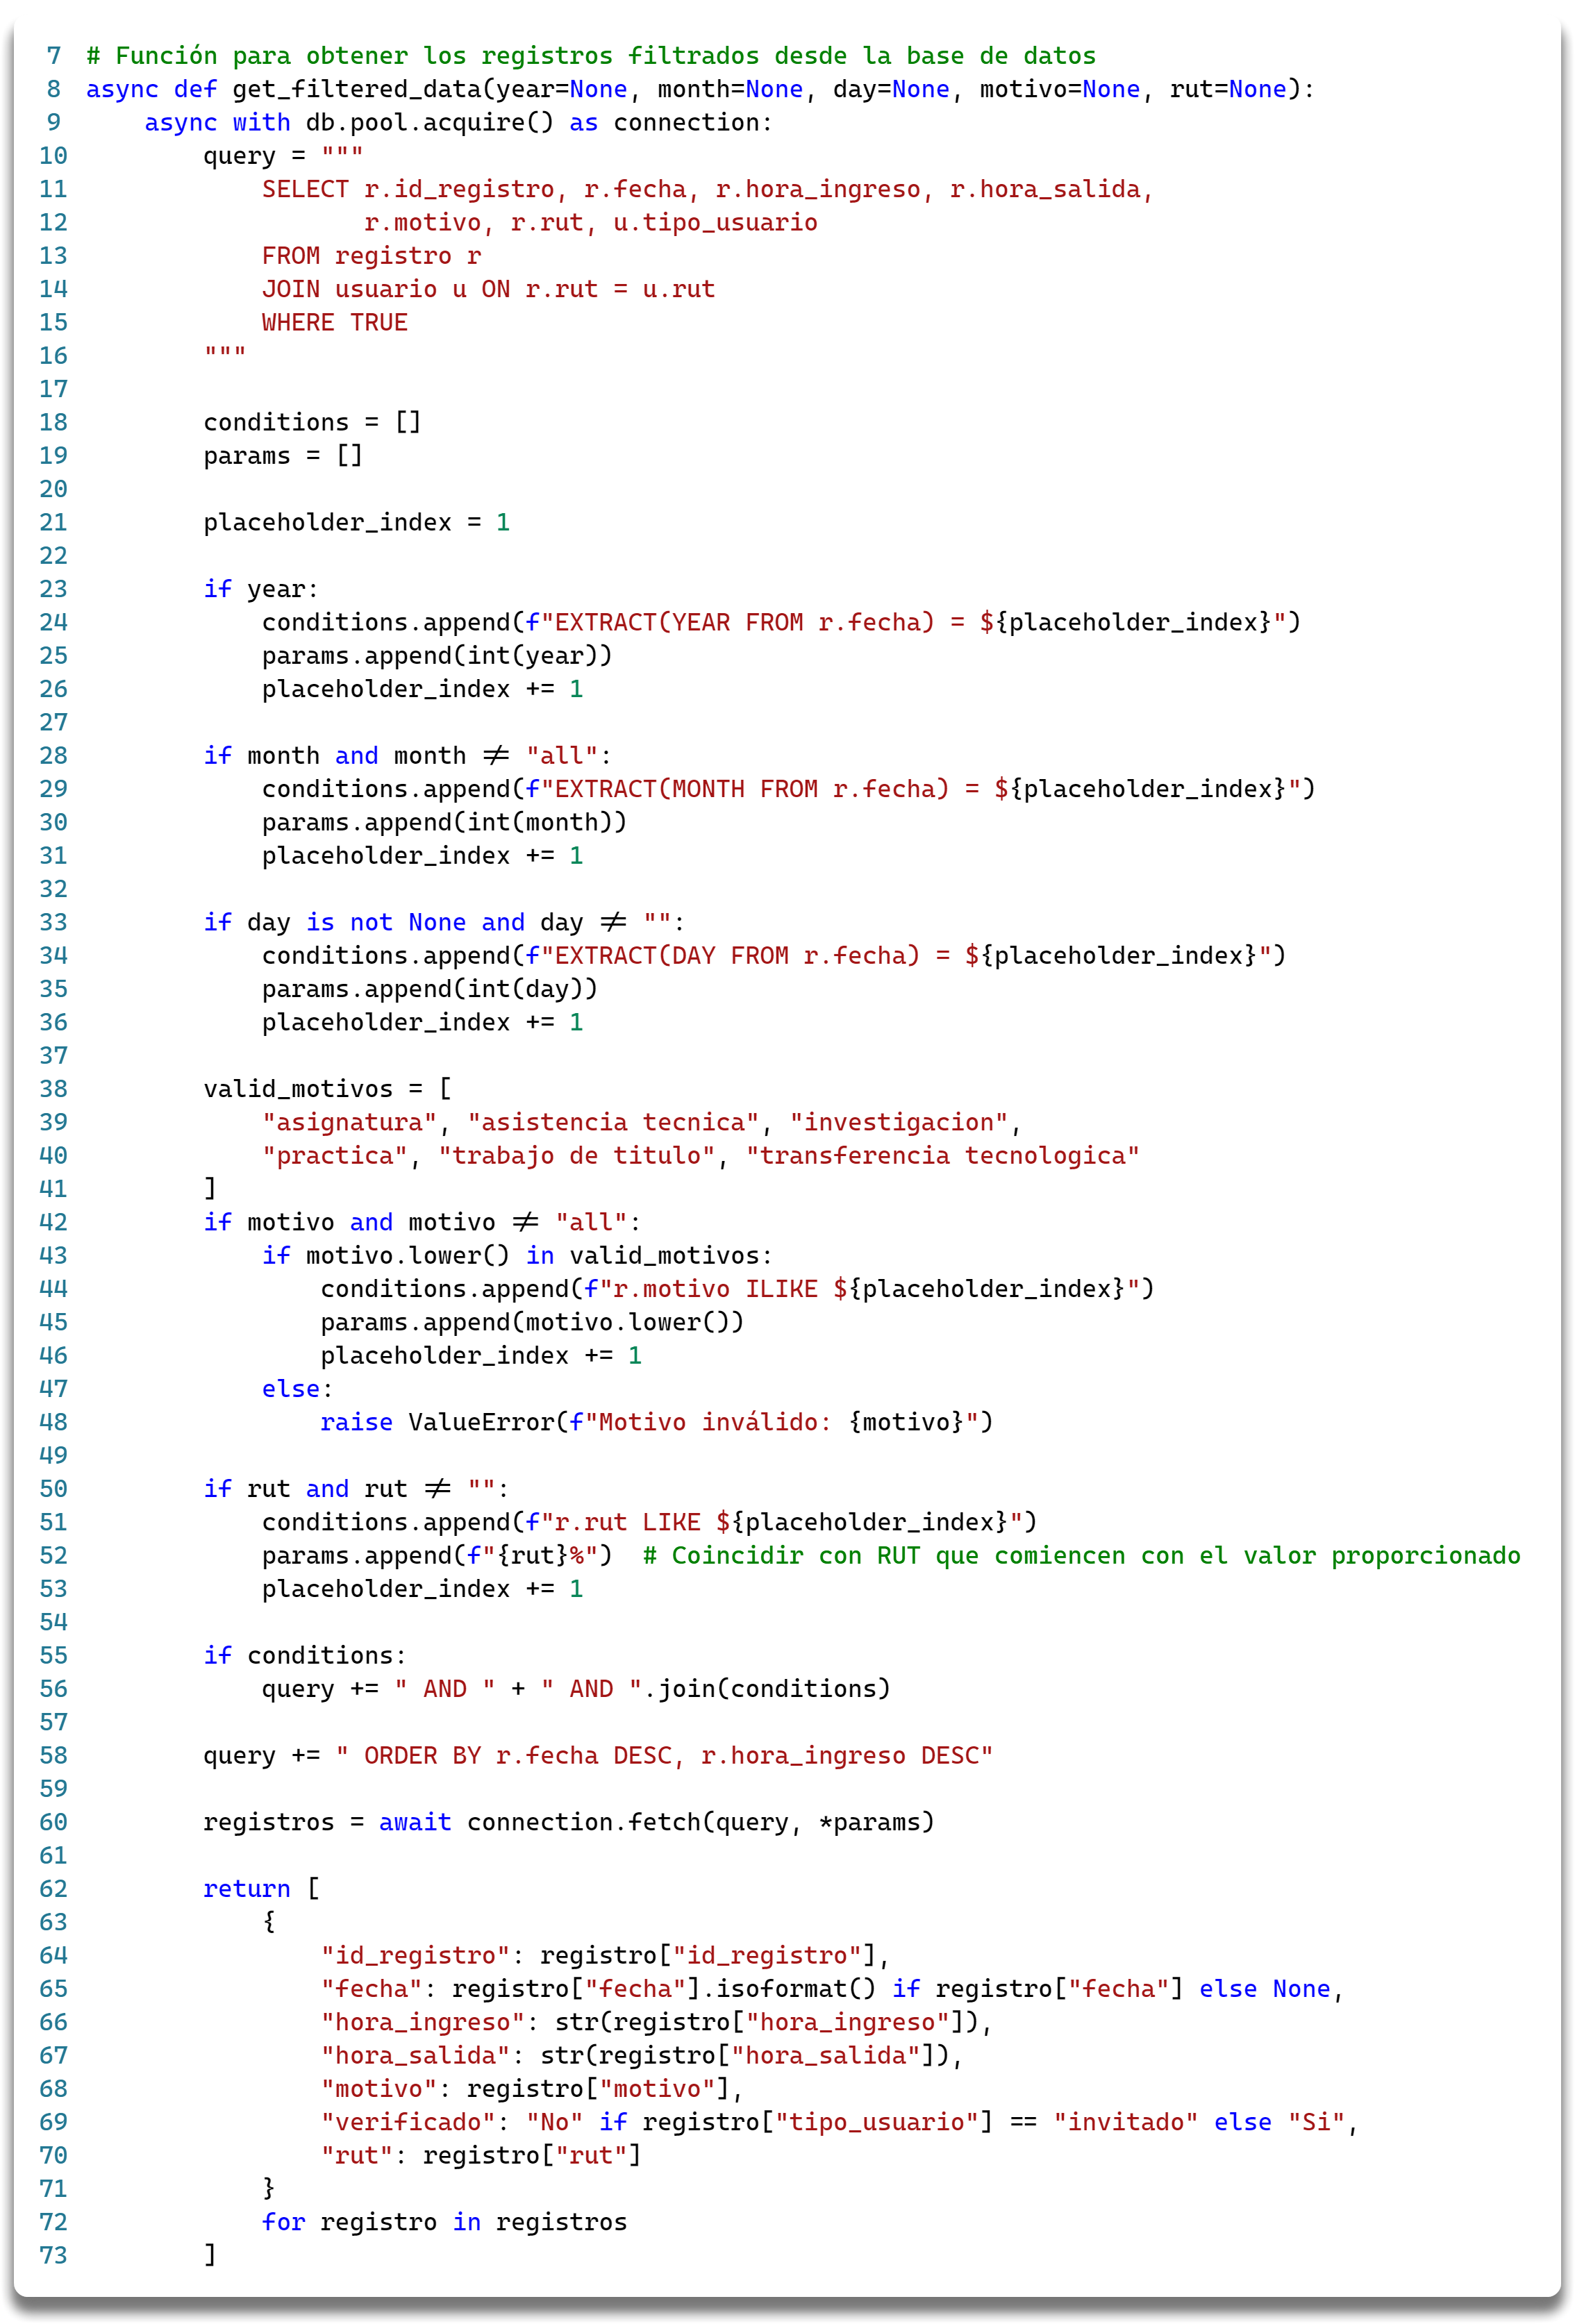
\includegraphics[width=0.9\textwidth]{img/query2.png}
			            \caption{Archivo query.py Parte II}
			            \label{fig:query2}
		            \end{figure}
		      \item Función que obtiene todos los registros de un rut entregado por parametros:
		            \begin{figure}[H]
			            \centering
			            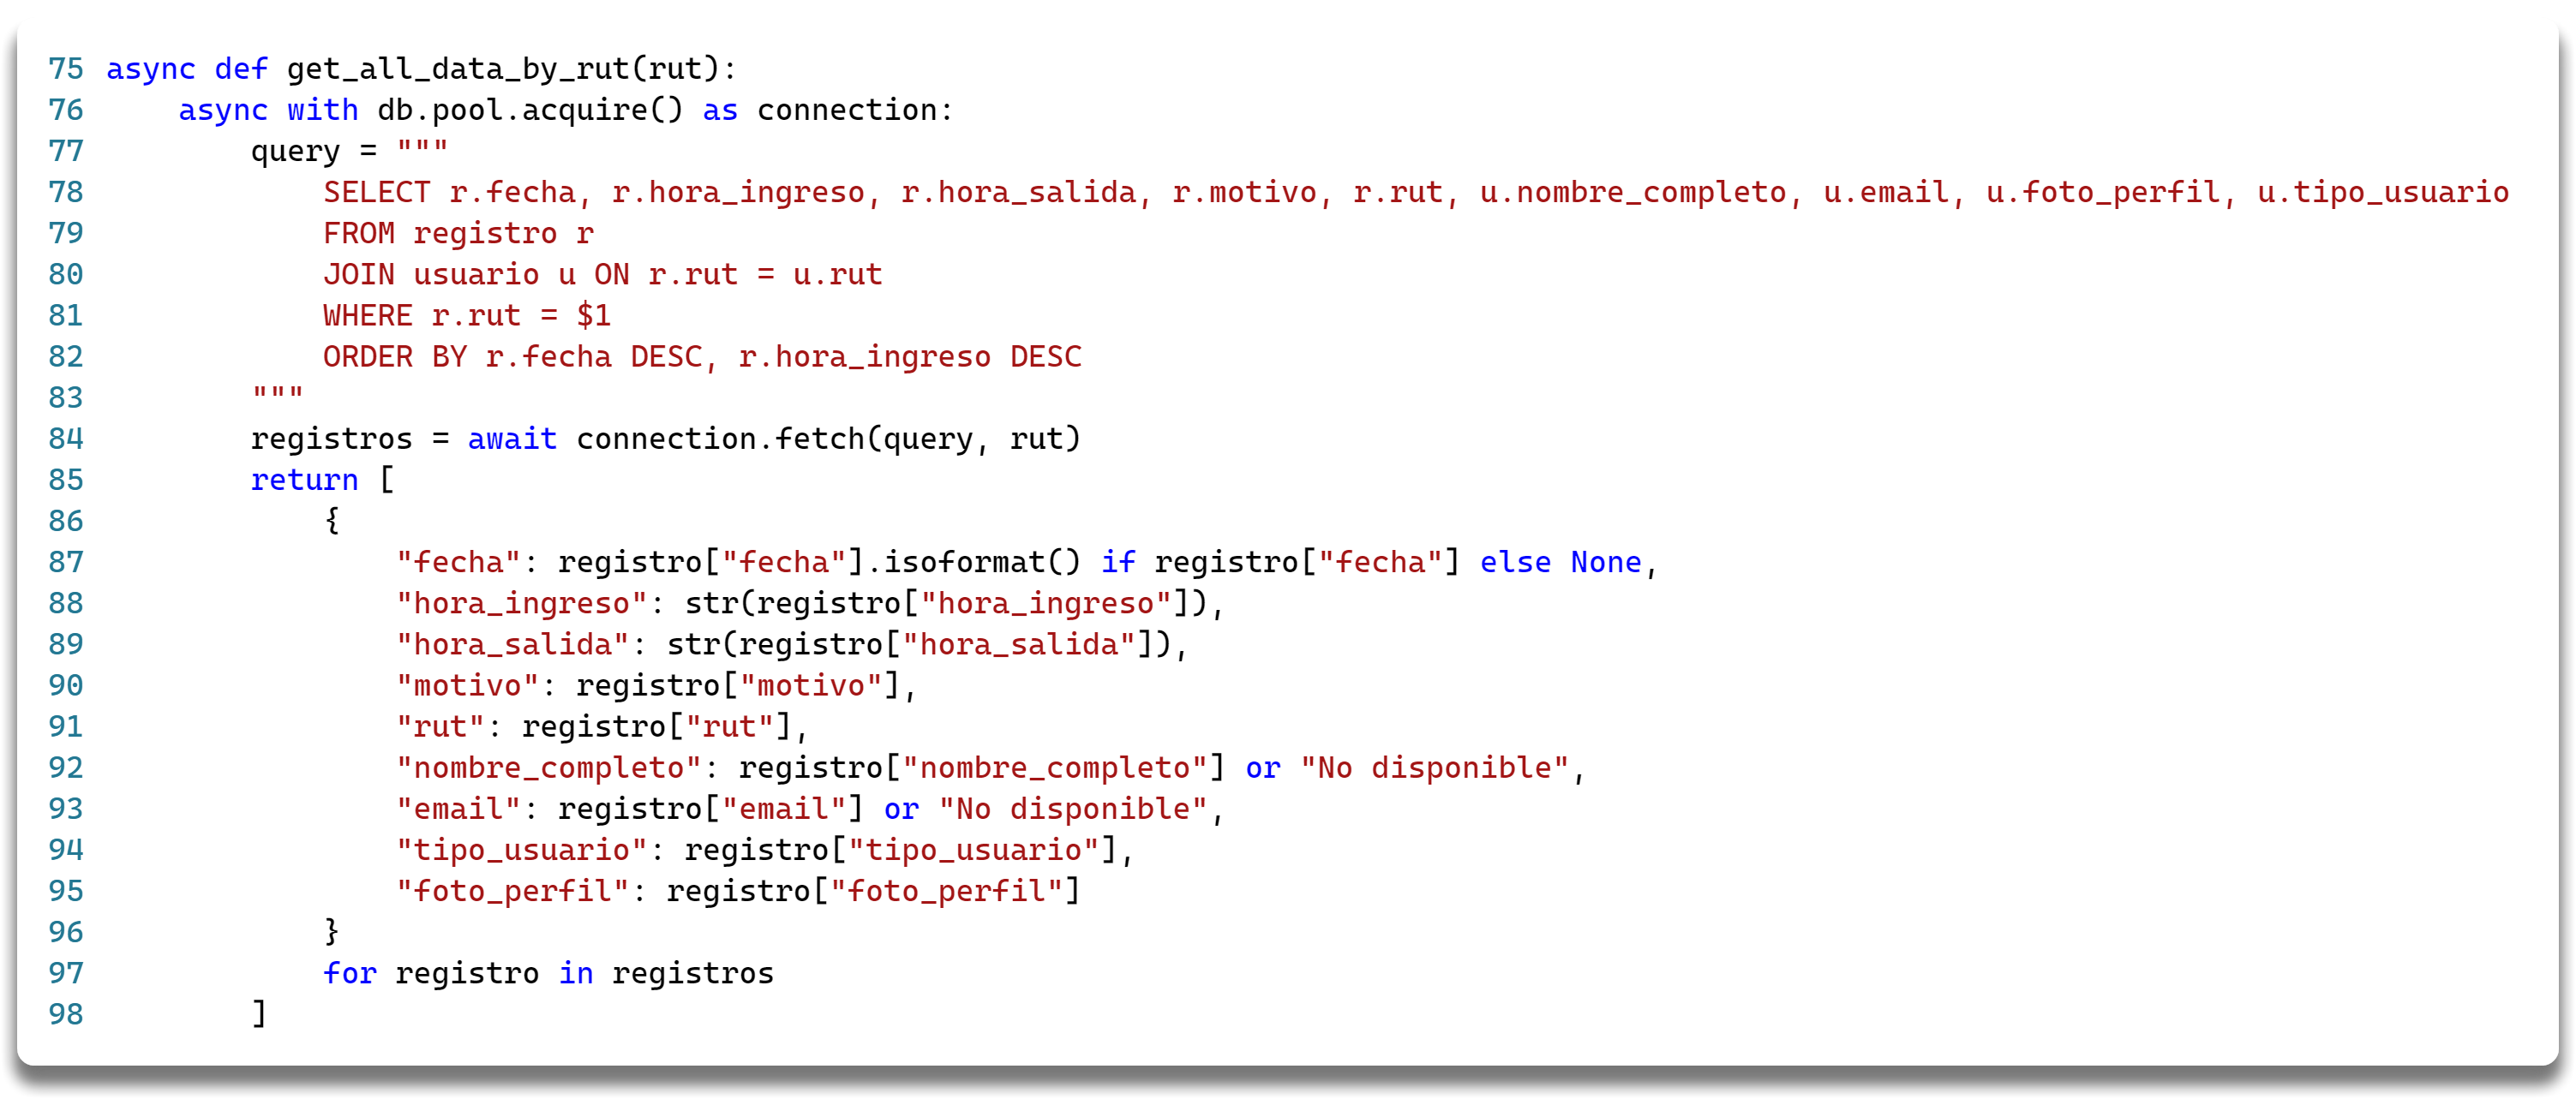
\includegraphics[width=\textwidth]{img/query3.png}
			            \caption{Archivo query.py Parte III}
			            \label{fig:query3}
		            \end{figure}
		      \item Función que verifica la existencia de un login, si no existe el objetivo es mostrarle al supervisor que las credenciales de ingreso son incorrectas:
		            \begin{figure}[H]
			            \centering
			            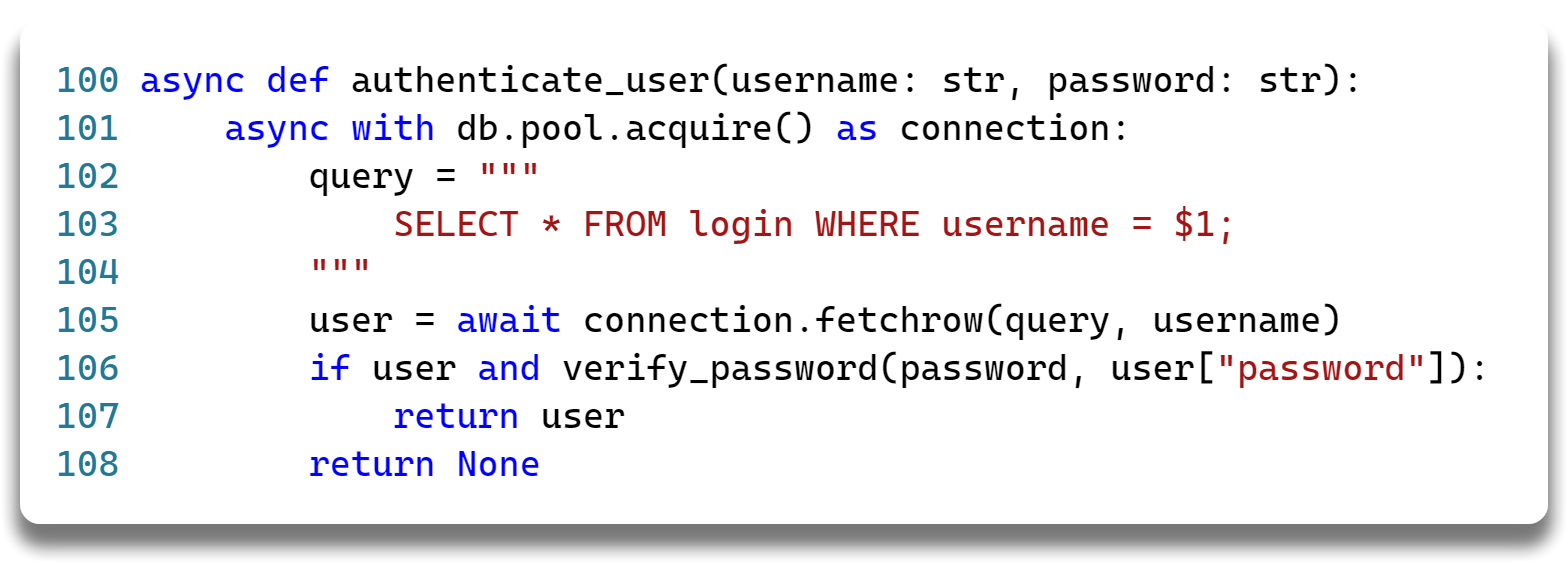
\includegraphics[width=0.75\textwidth]{img/query4.png}
			            \caption{Archivo query.py Parte IV}
			            \label{fig:query4}
		            \end{figure}
		            \newpage
		      \item Función que se encarga de obtener los mensajes de la DB, esto para notificar en la aplicación web de ingresos o salidas según corresponda:
		            \begin{figure}[H]
			            \centering
			            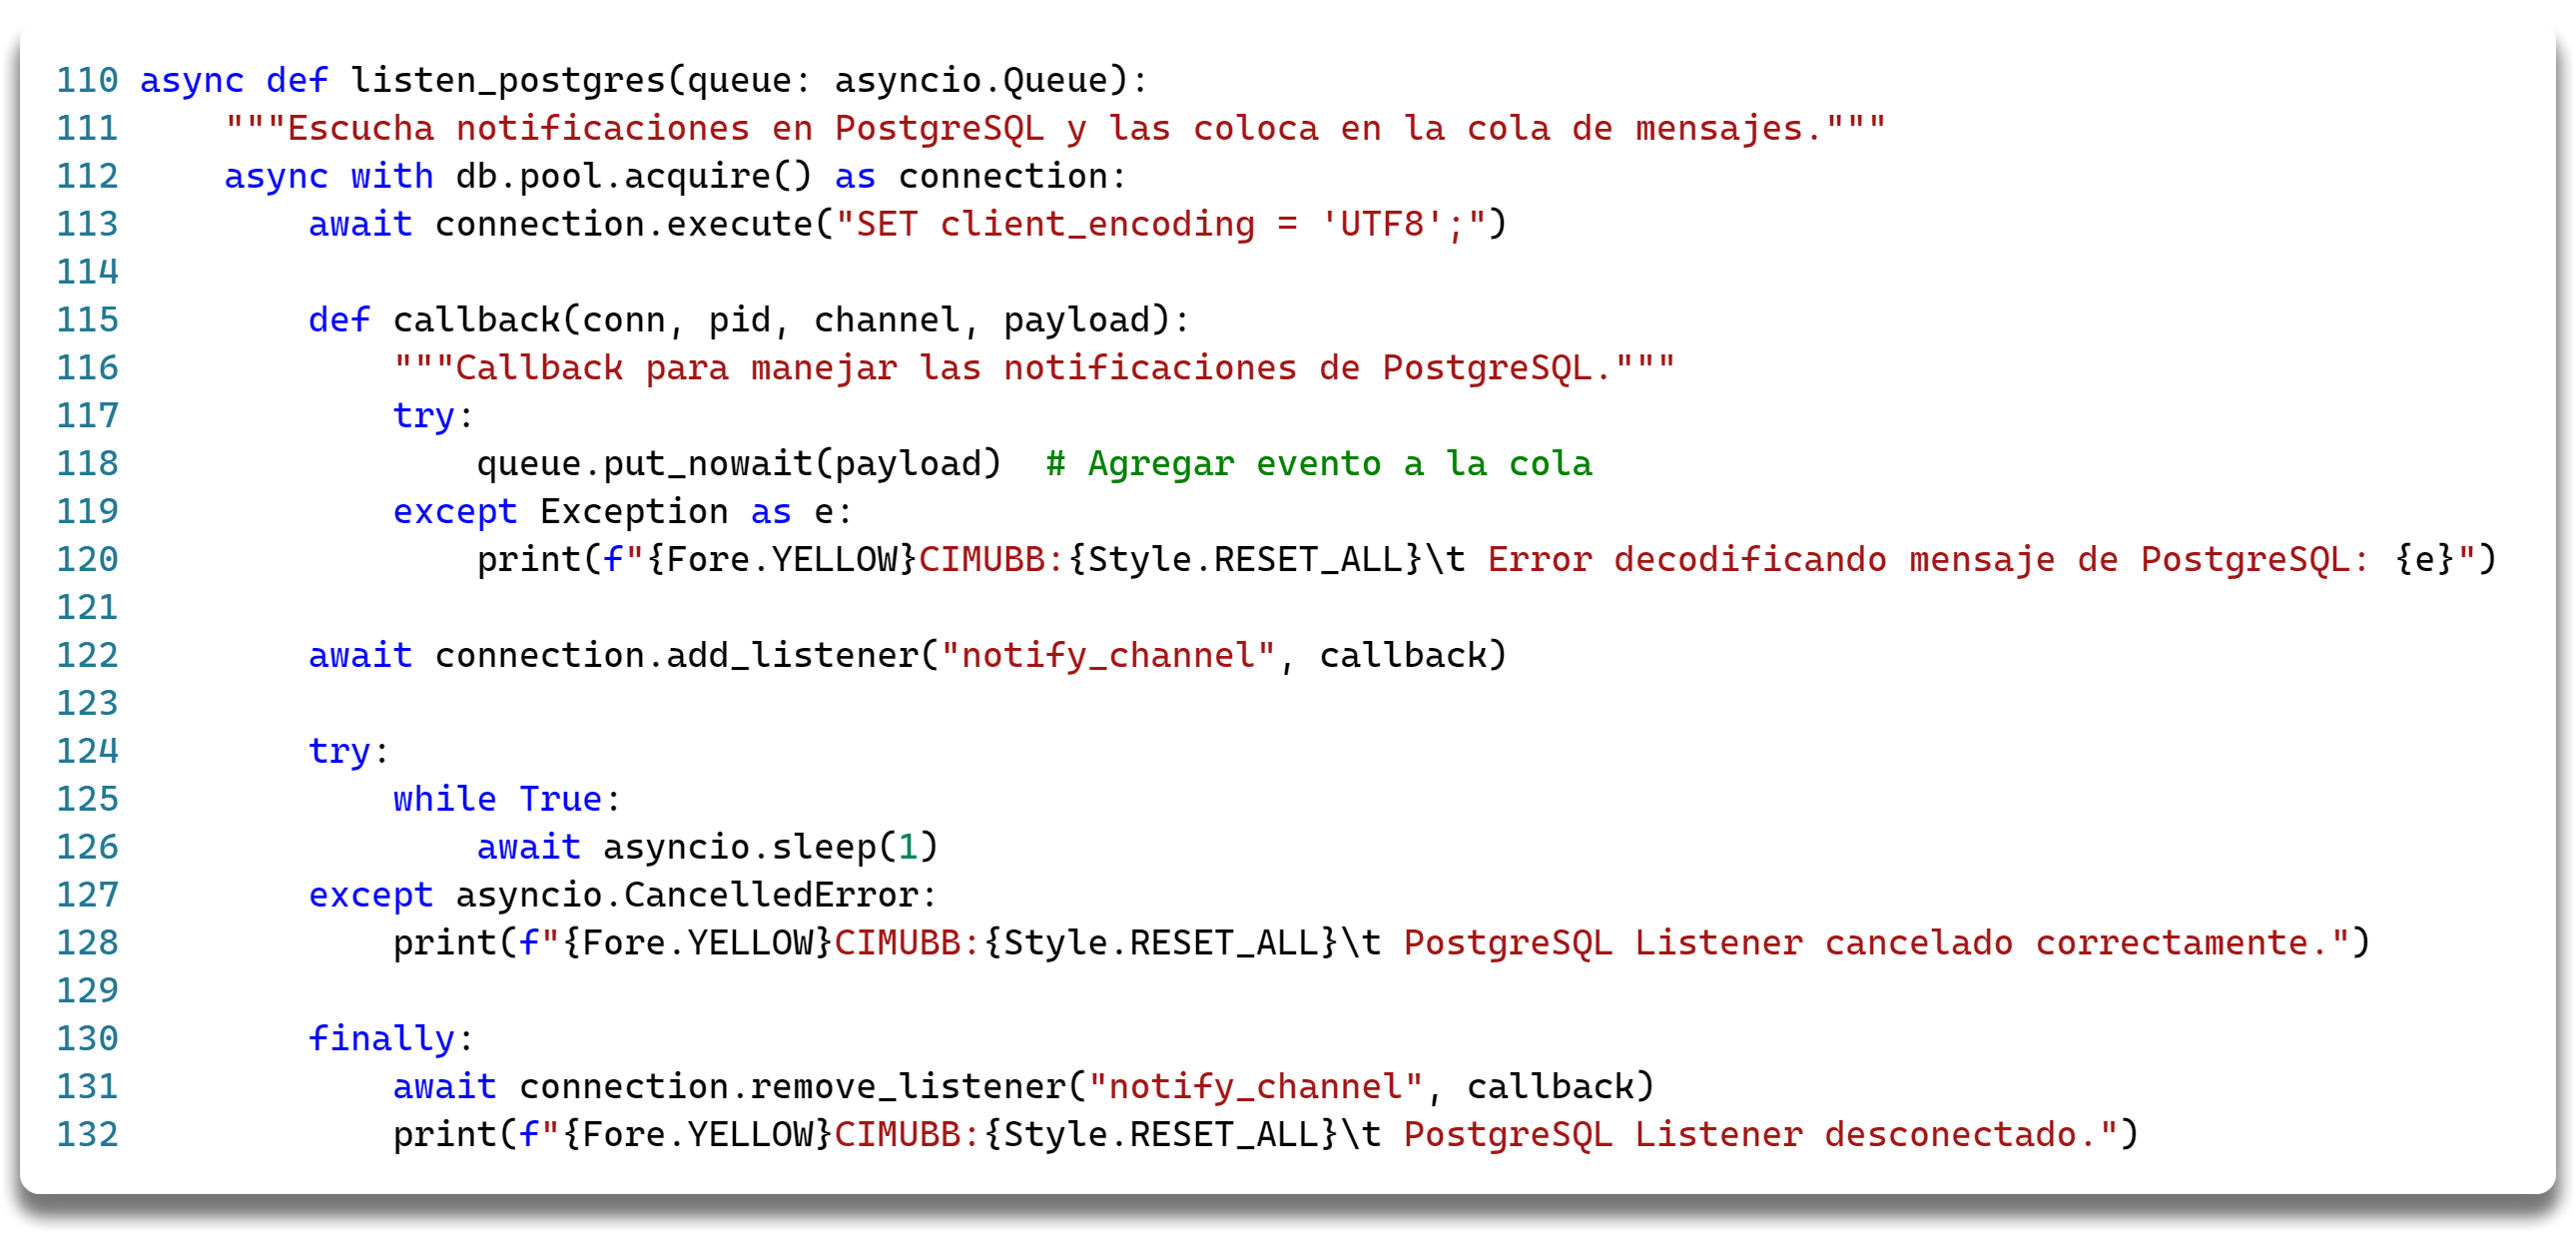
\includegraphics[width=\textwidth]{img/query5.png}
			            \caption{Archivo query.py Parte V}
			            \label{fig:query5}
		            \end{figure}
	      \end{enumerate}

	\item \textbf{main.py}:
	      \begin{enumerate}
		      \item Importación de librerías <<inserte calavera>>:
		            \begin{figure}[H]
			            \centering
			            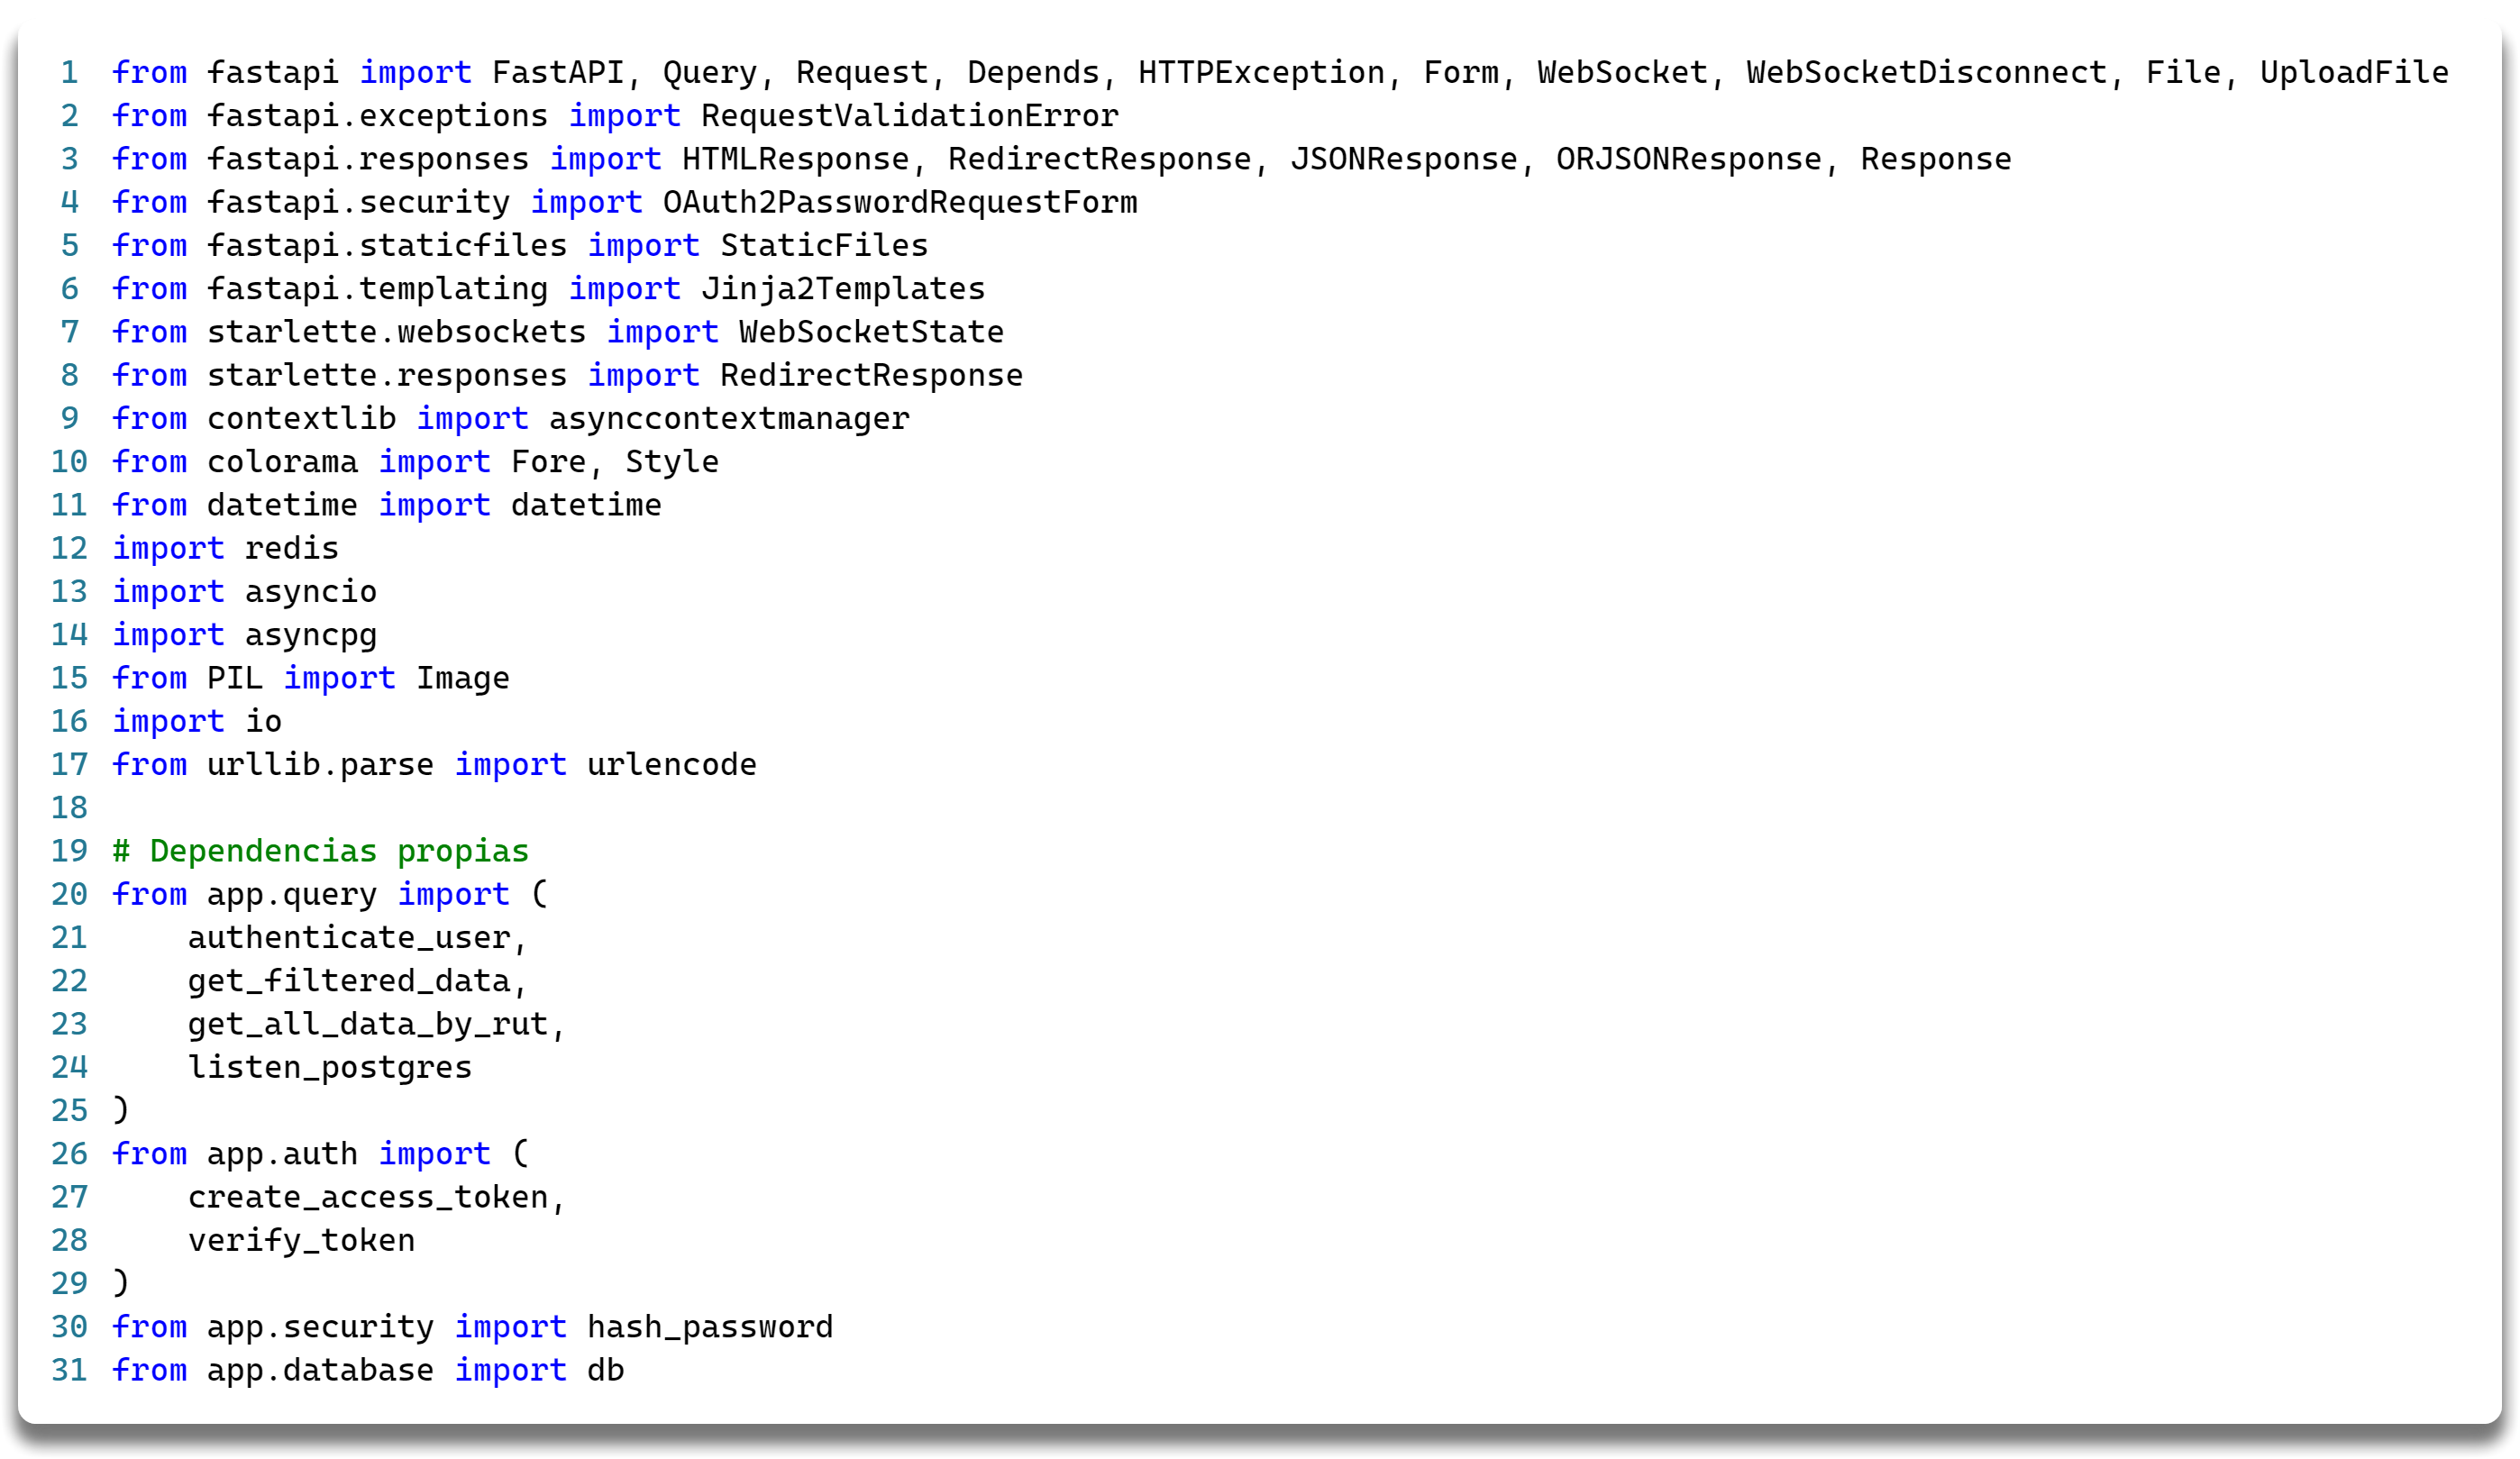
\includegraphics[width=\textwidth]{img/main1.png}
			            \caption{Archivo main.py Parte I}
			            \label{fig:main1}
		            \end{figure}
		            \newpage
		      \item Conexión con redis para manejar la cola de notificaciones:
		            \begin{figure}[H]
			            \centering
			            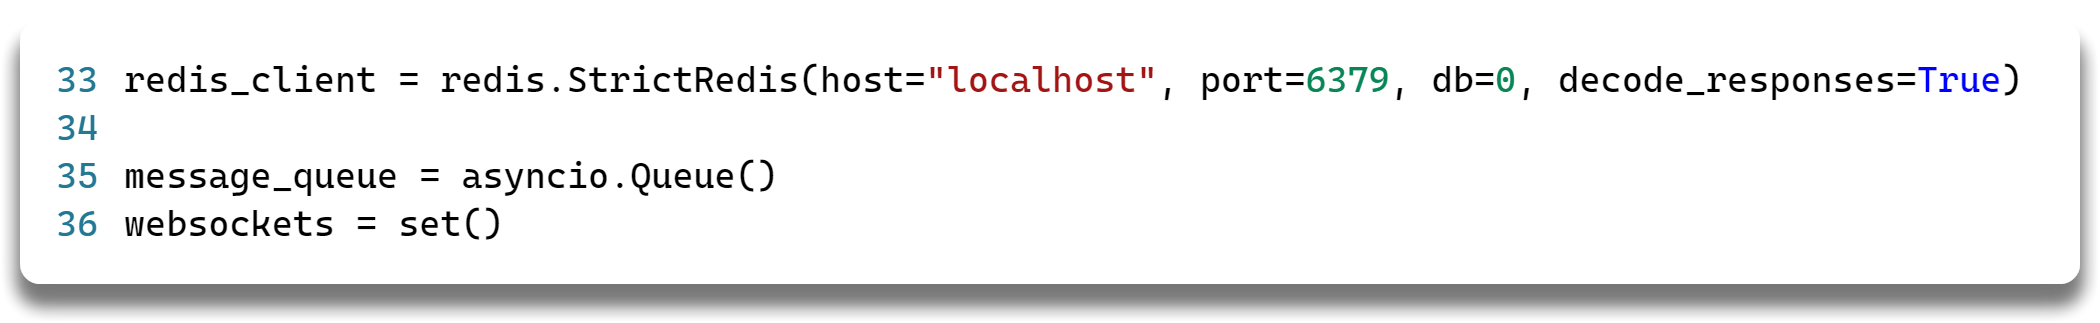
\includegraphics[width=\textwidth]{img/main2.png}
			            \caption{Archivo main.py Parte II}
			            \label{fig:main2}
		            \end{figure}

		      \item Función que decide si envia las notificaciones directamente a los WebSockets activos, de lo contrario los guardara temporalmente en redis:
		            \begin{figure}[H]
			            \centering
			            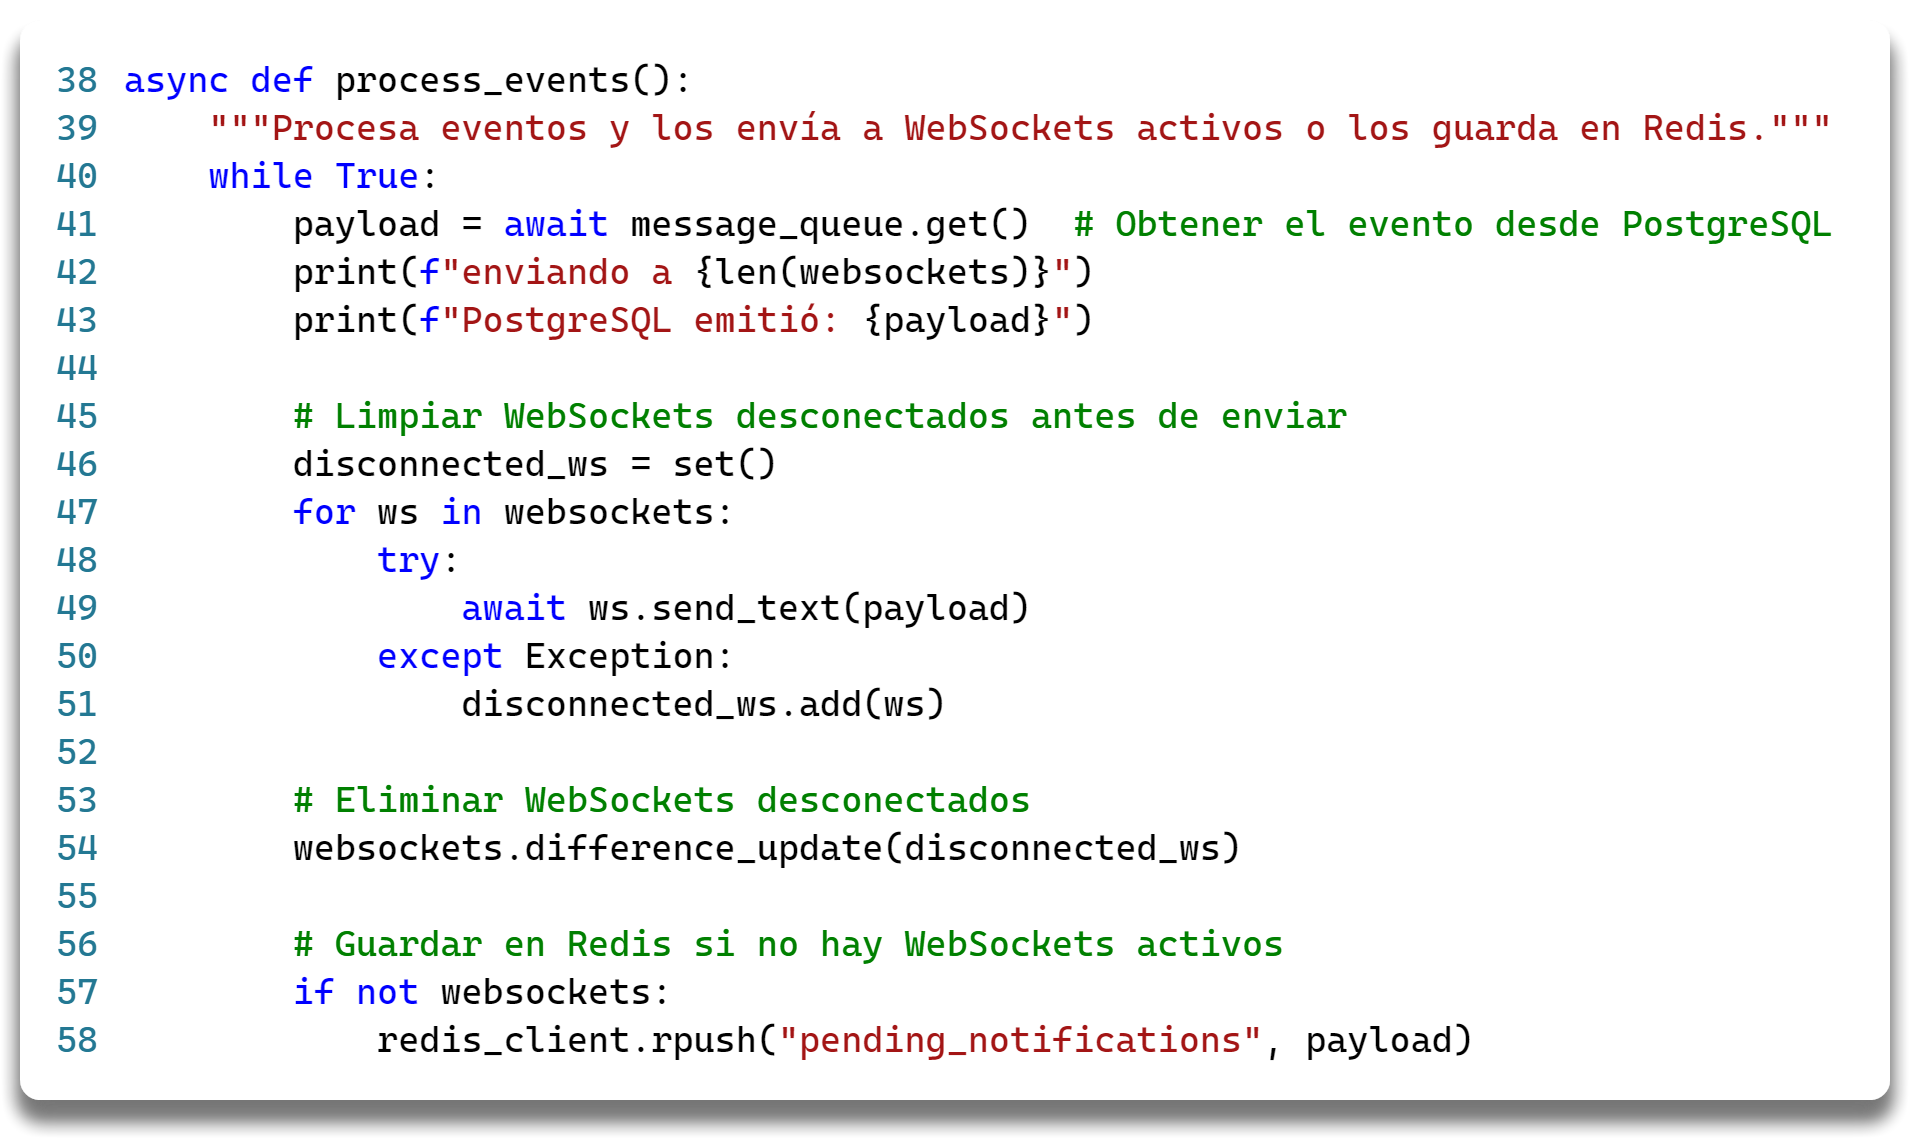
\includegraphics[width=\textwidth]{img/main3.png}
			            \caption{Archivo main.py Parte III}
			            \label{fig:main3}
		            \end{figure}
		      \item Función que valida el formato de la imagen pasada por parametros en el endpoint de register-user:
		            \begin{figure}[H]
			            \centering
			            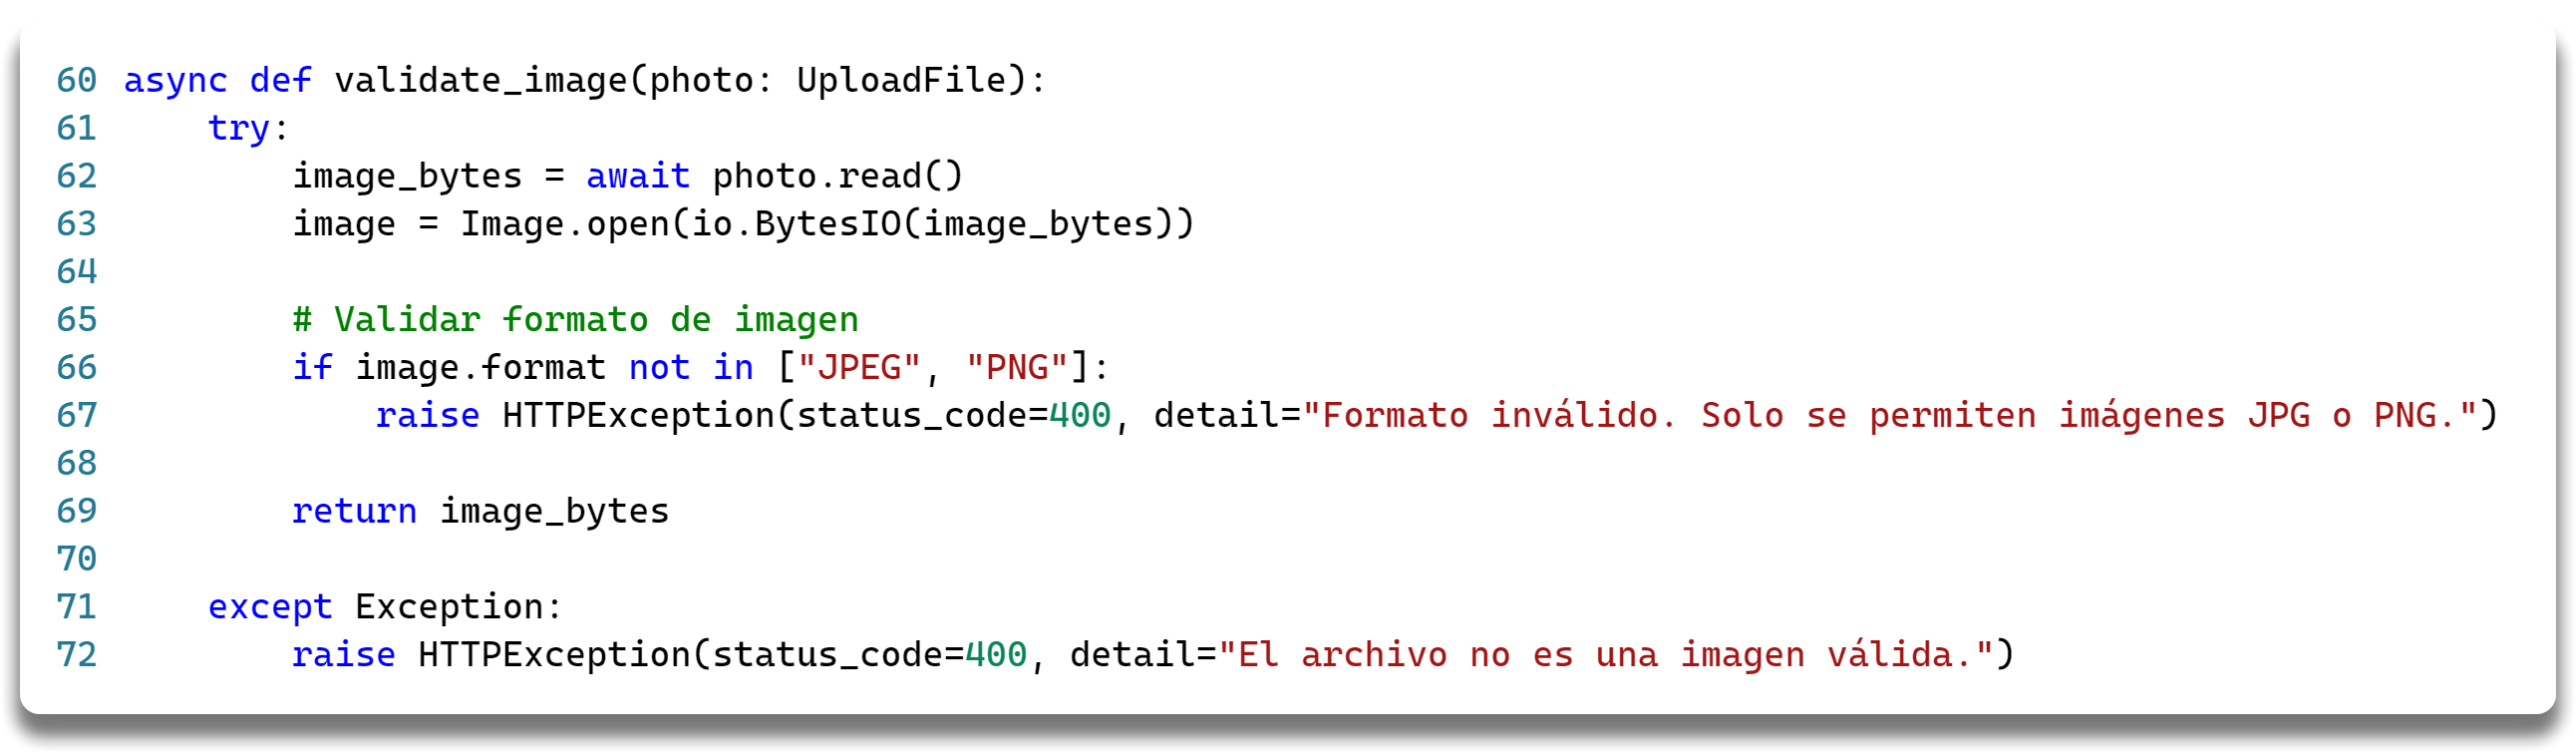
\includegraphics[width=\textwidth]{img/main4.png}
			            \caption{Archivo main.py Parte IV}
			            \label{fig:main4}
		            \end{figure}
		            \newpage
		      \item Control del ciclo de vida del software, que permite controlar y detener funciones si es que se detiene el SW:
		            \begin{figure}[H]
			            \centering
			            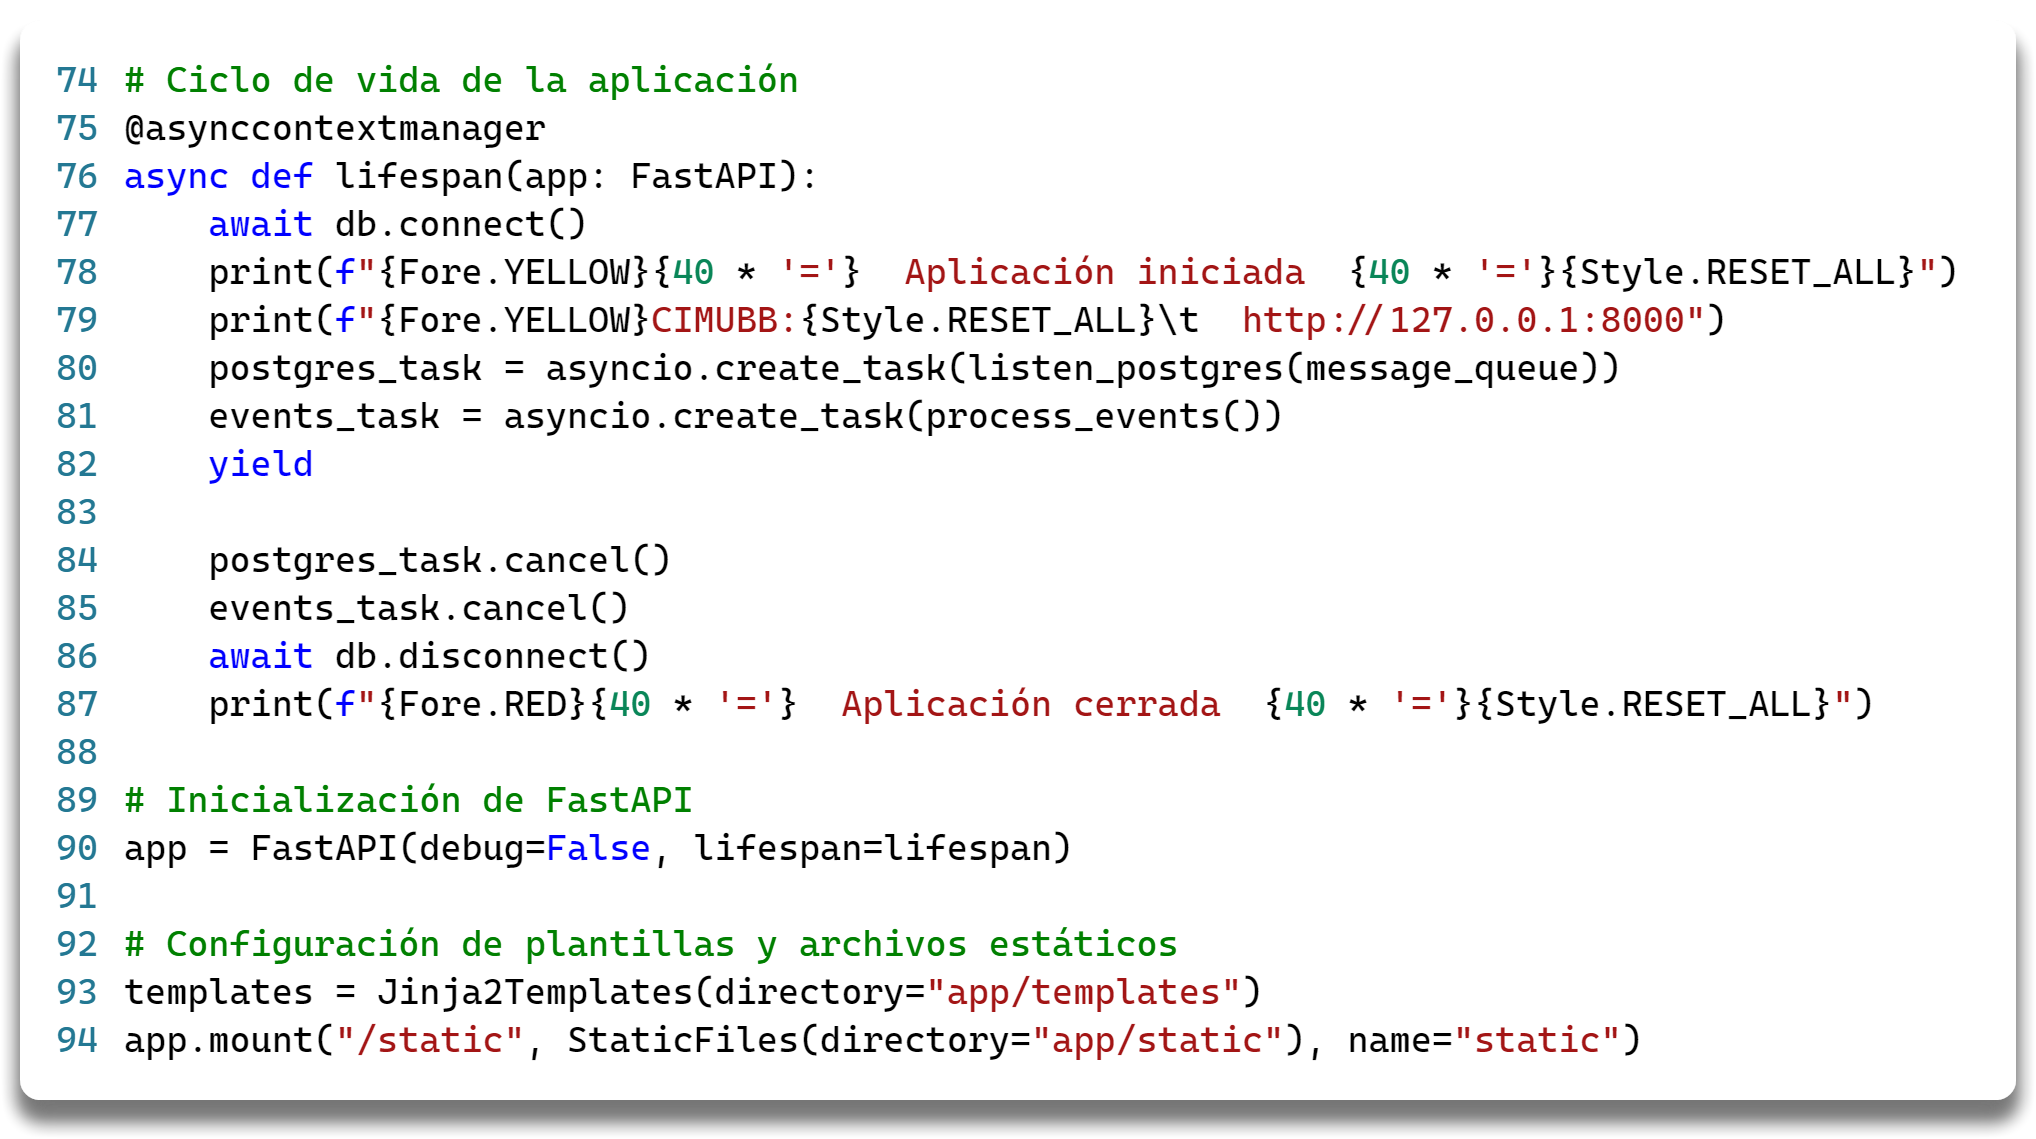
\includegraphics[width=\textwidth]{img/main5.png}
			            \caption{Archivo main.py Parte V}
			            \label{fig:main5}
		            \end{figure}

		      \item Importación de CORS y definici\'on de rutas protegidas:
		            \begin{figure}[H]
			            \centering
			            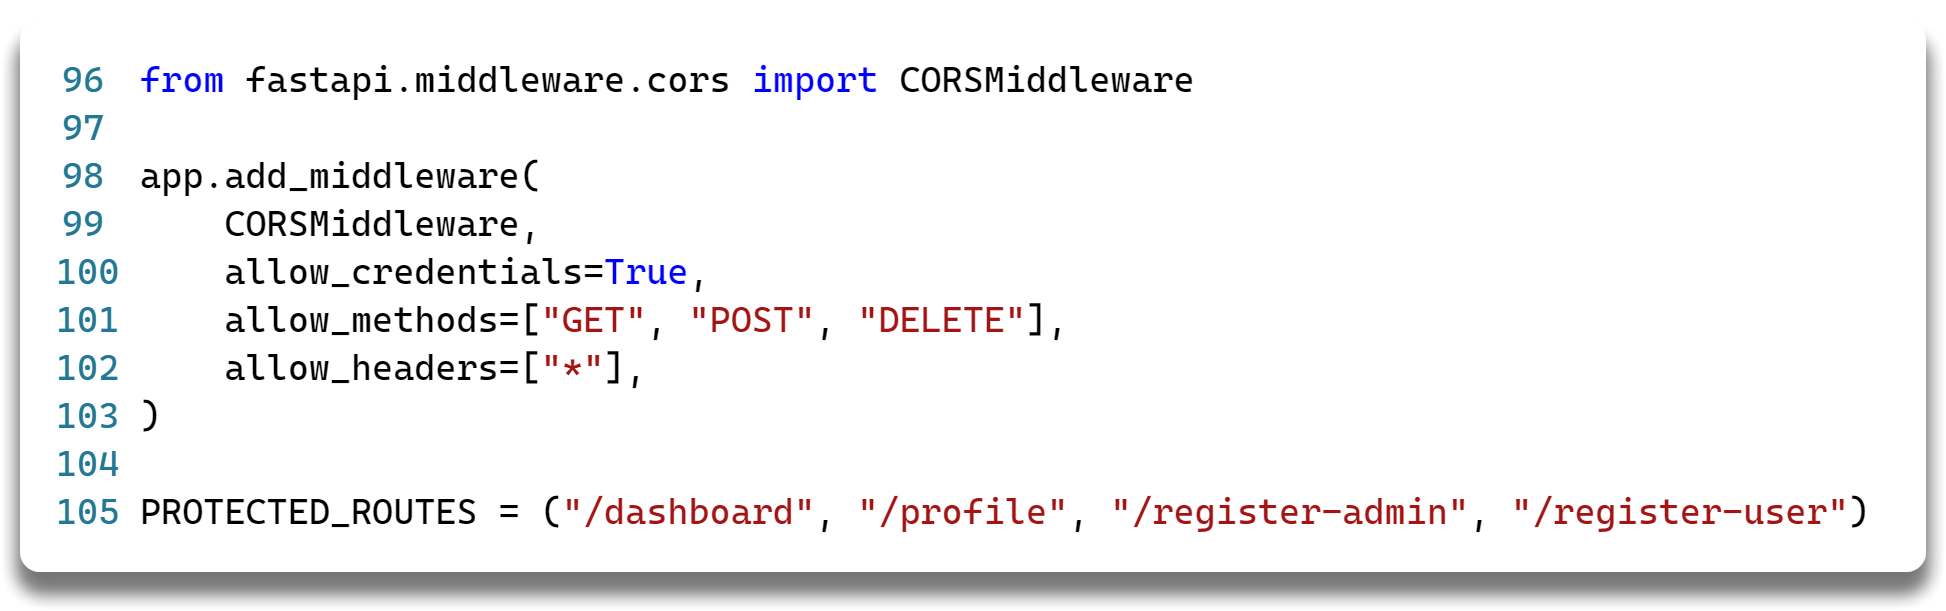
\includegraphics[width=\textwidth]{img/main6.png}
			            \caption{Archivo main.py Parte VI}
			            \label{fig:main6}
		            \end{figure}
		            \newpage
		      \item Protecci\'on del middleware, para permitir el acceso a URL especificas solo si esta validado su JWT:
		            \begin{figure}[H]
			            \centering
			            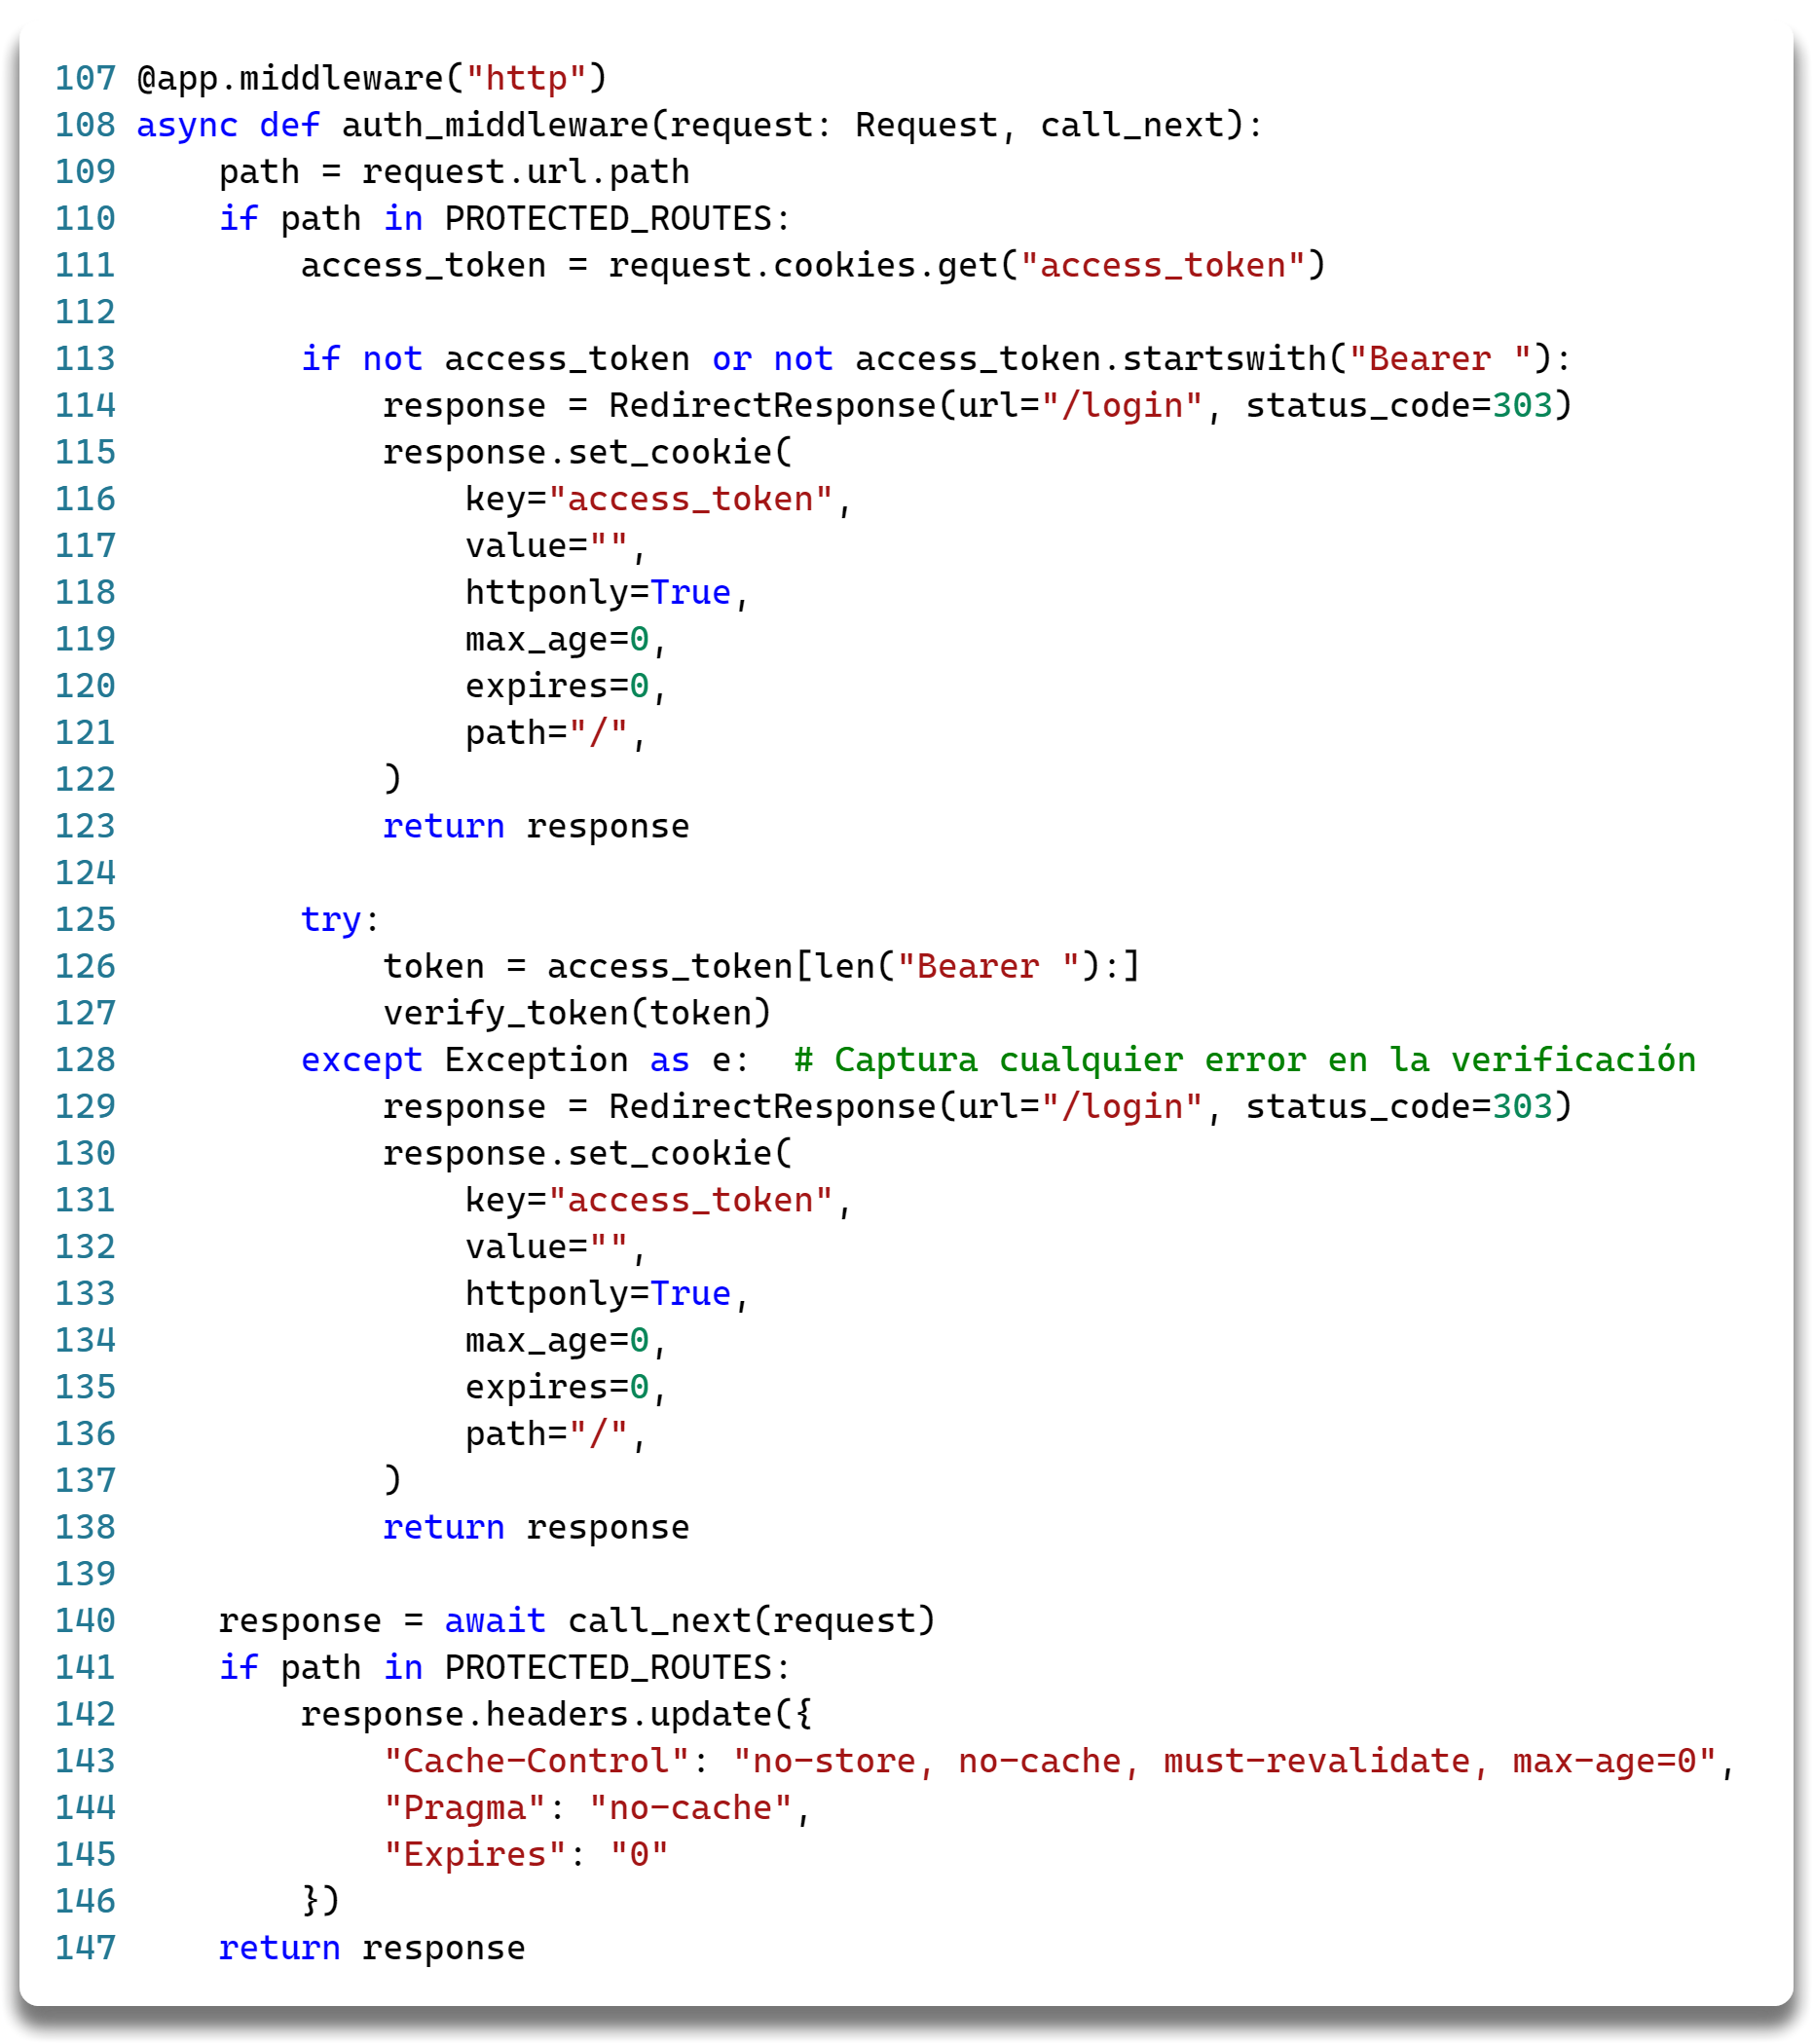
\includegraphics[width=\textwidth]{img/main7.png}
			            \caption{Archivo main.py Parte VII}
			            \label{fig:main7}
		            \end{figure}
		            \newpage
		      \item Endpoint que entrega p\'aginas html est\'aticas:
		            \begin{figure}[H]
			            \centering
			            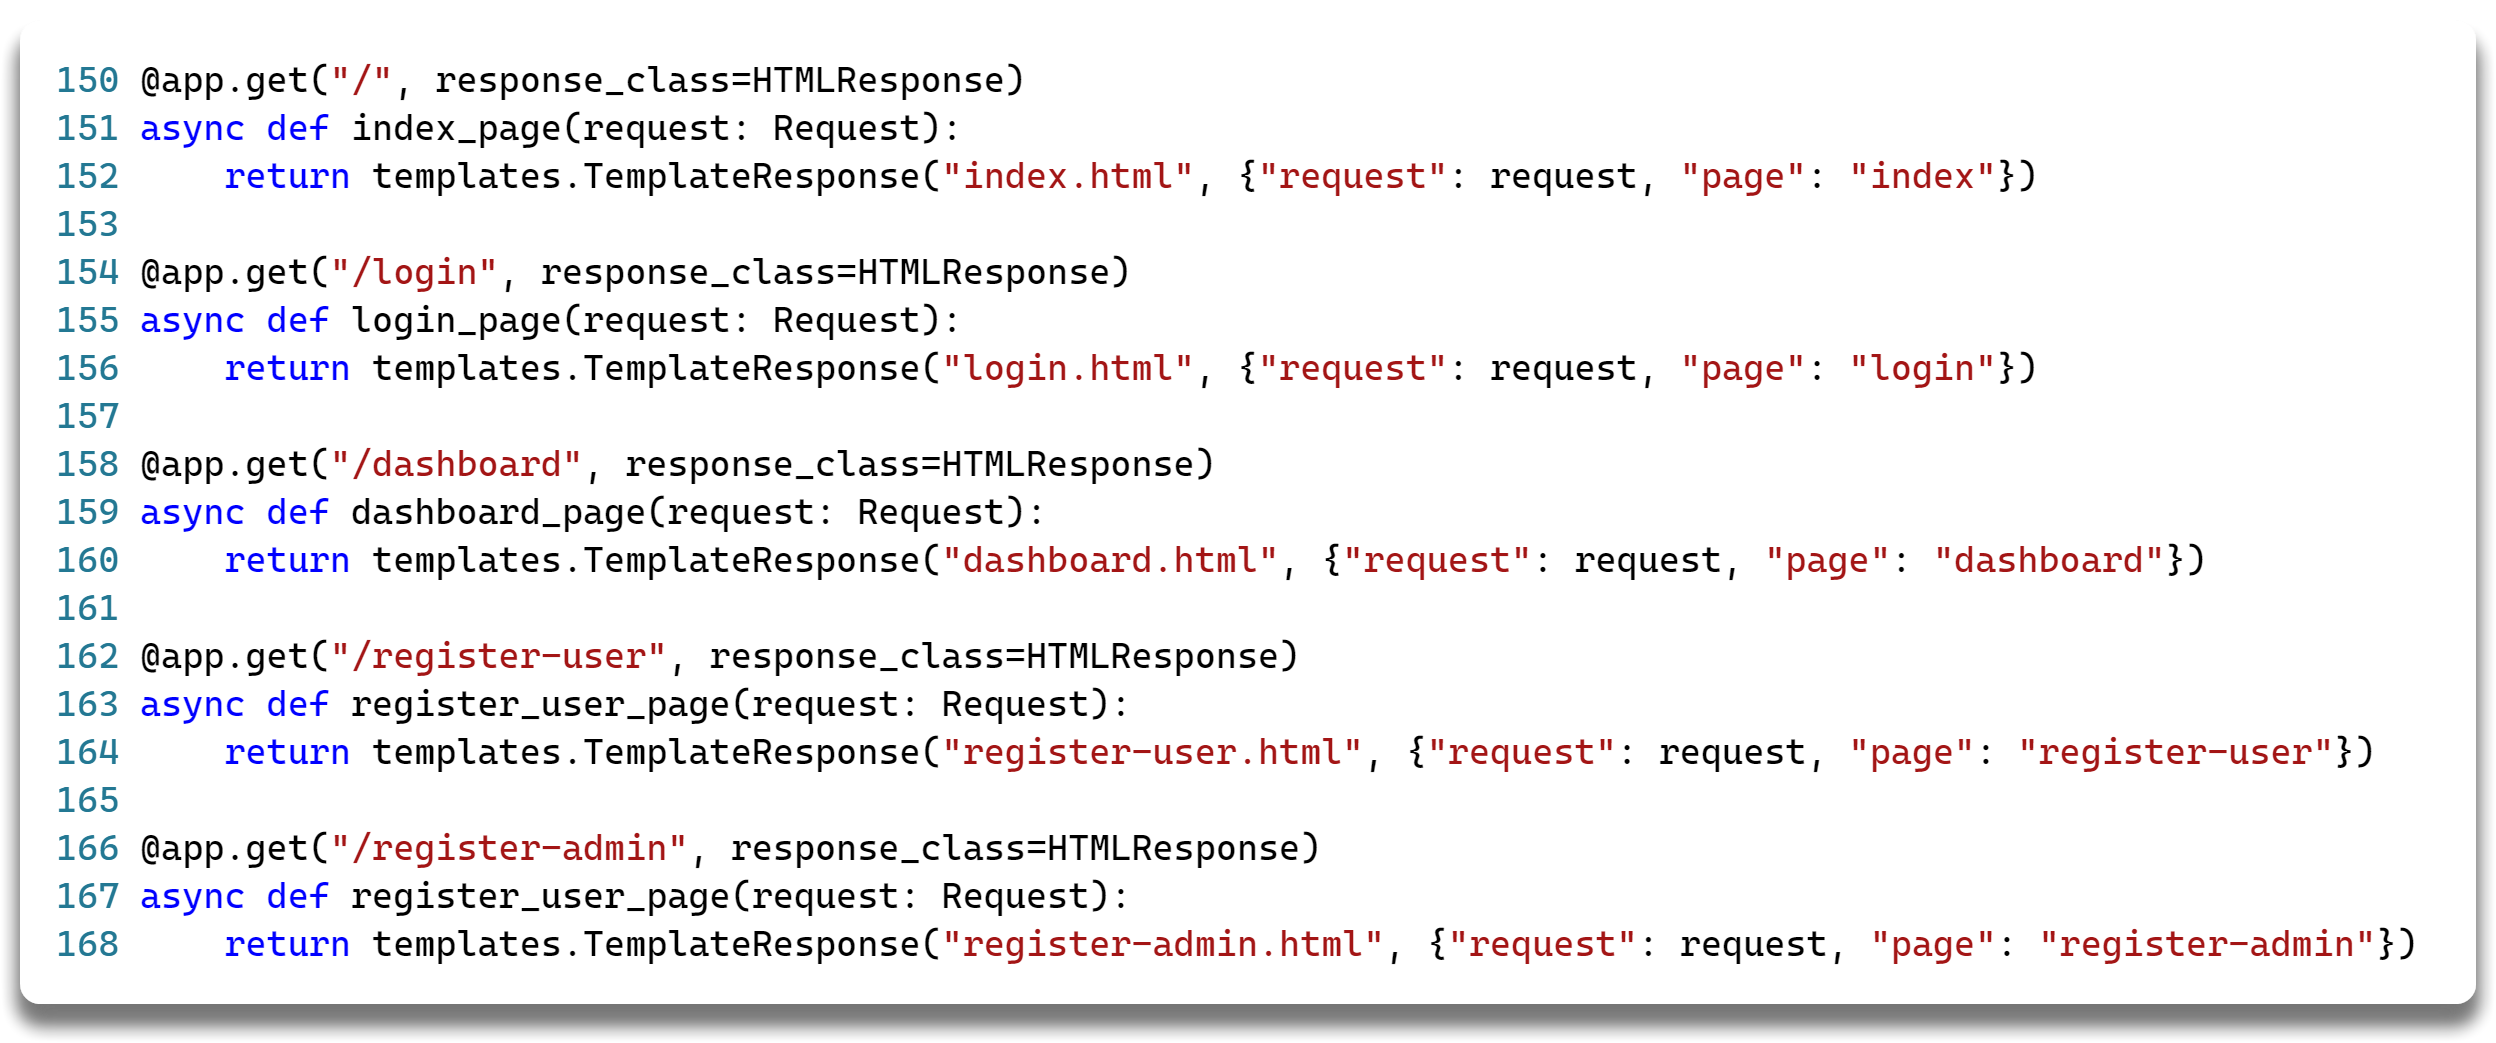
\includegraphics[width=\textwidth]{img/main8.png}
			            \caption{Archivo main.py Parte VIII}
			            \label{fig:main8}
		            \end{figure}

		      \item Endpoint para facilitar el acceso a im\'agenes de perfil que pueda poseer un usuario:
		            \begin{figure}[H]
			            \centering
			            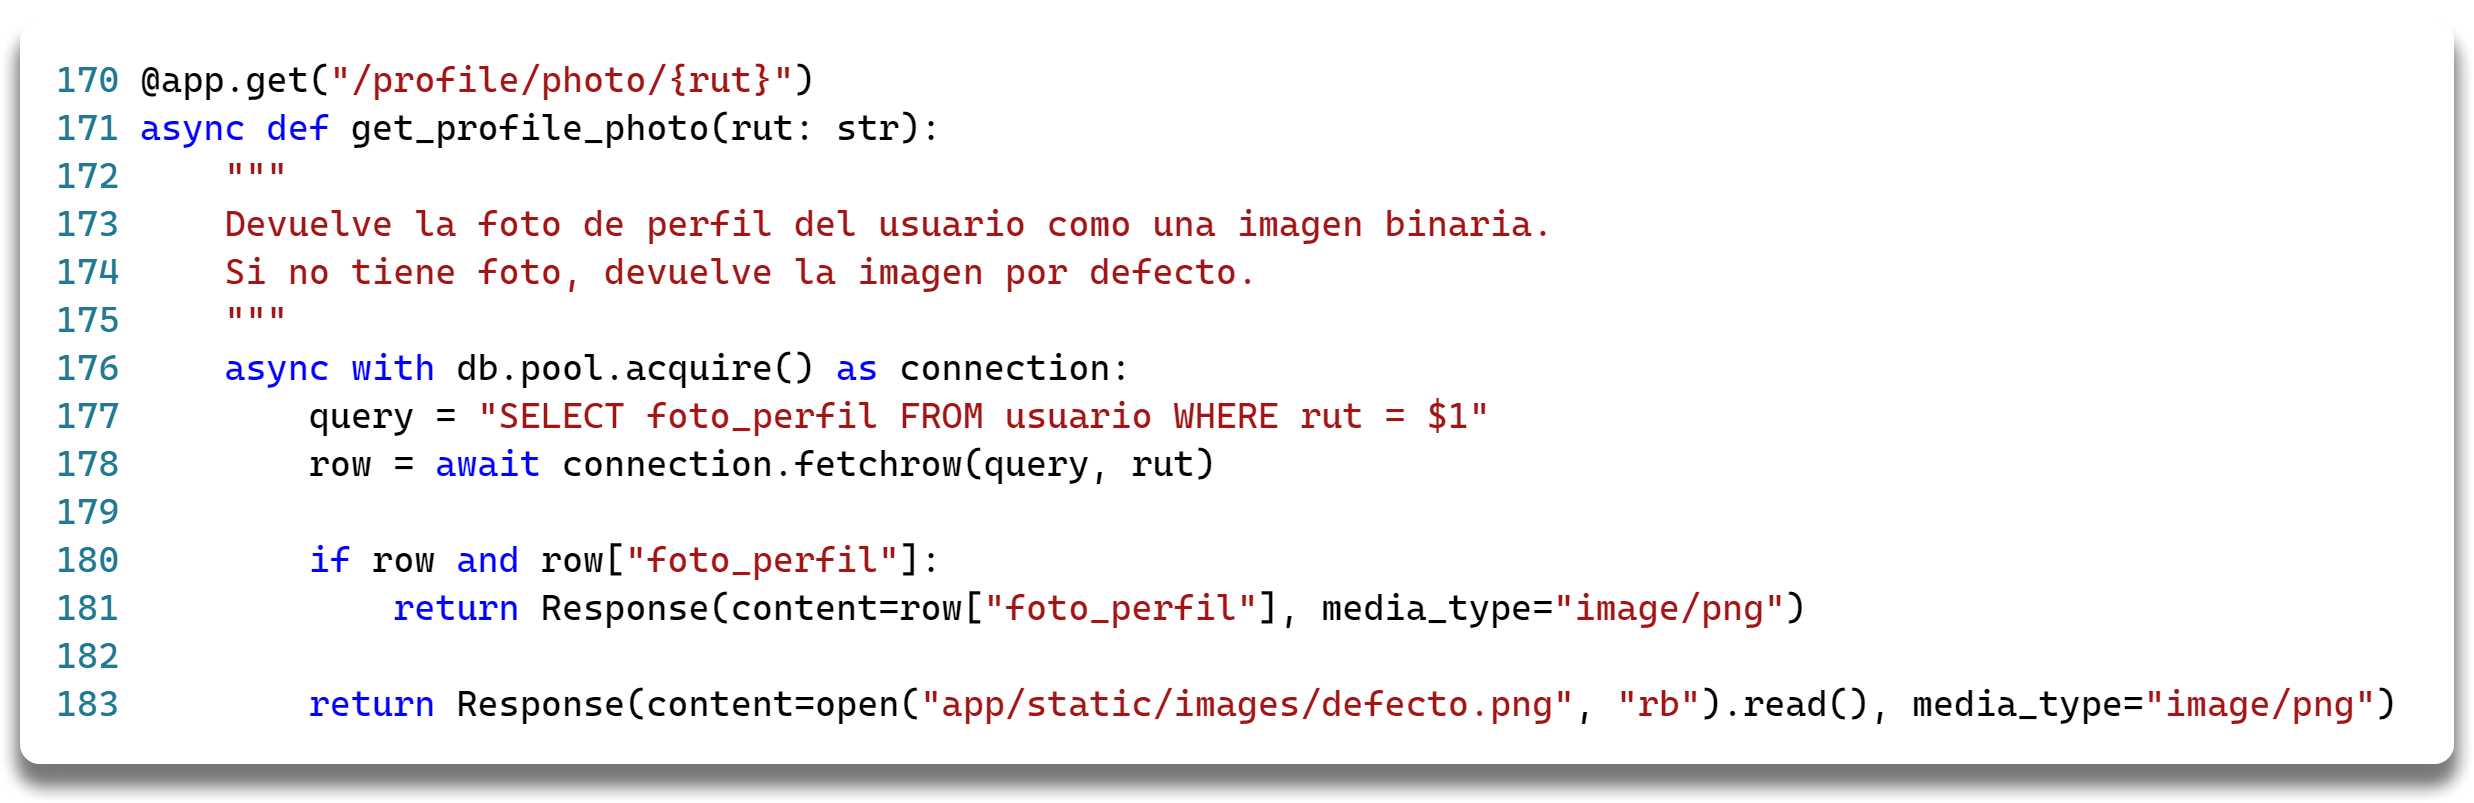
\includegraphics[width=\textwidth]{img/main9.png}
			            \caption{Archivo main.py Parte IX}
			            \label{fig:main9}
		            \end{figure}
		            \newpage
		      \item Endpoint para mostrar la p\'agina web din\'amica profile, la que mediante un rut muestra todos los registros de ese usuario:
		            \begin{figure}[H]
			            \centering
			            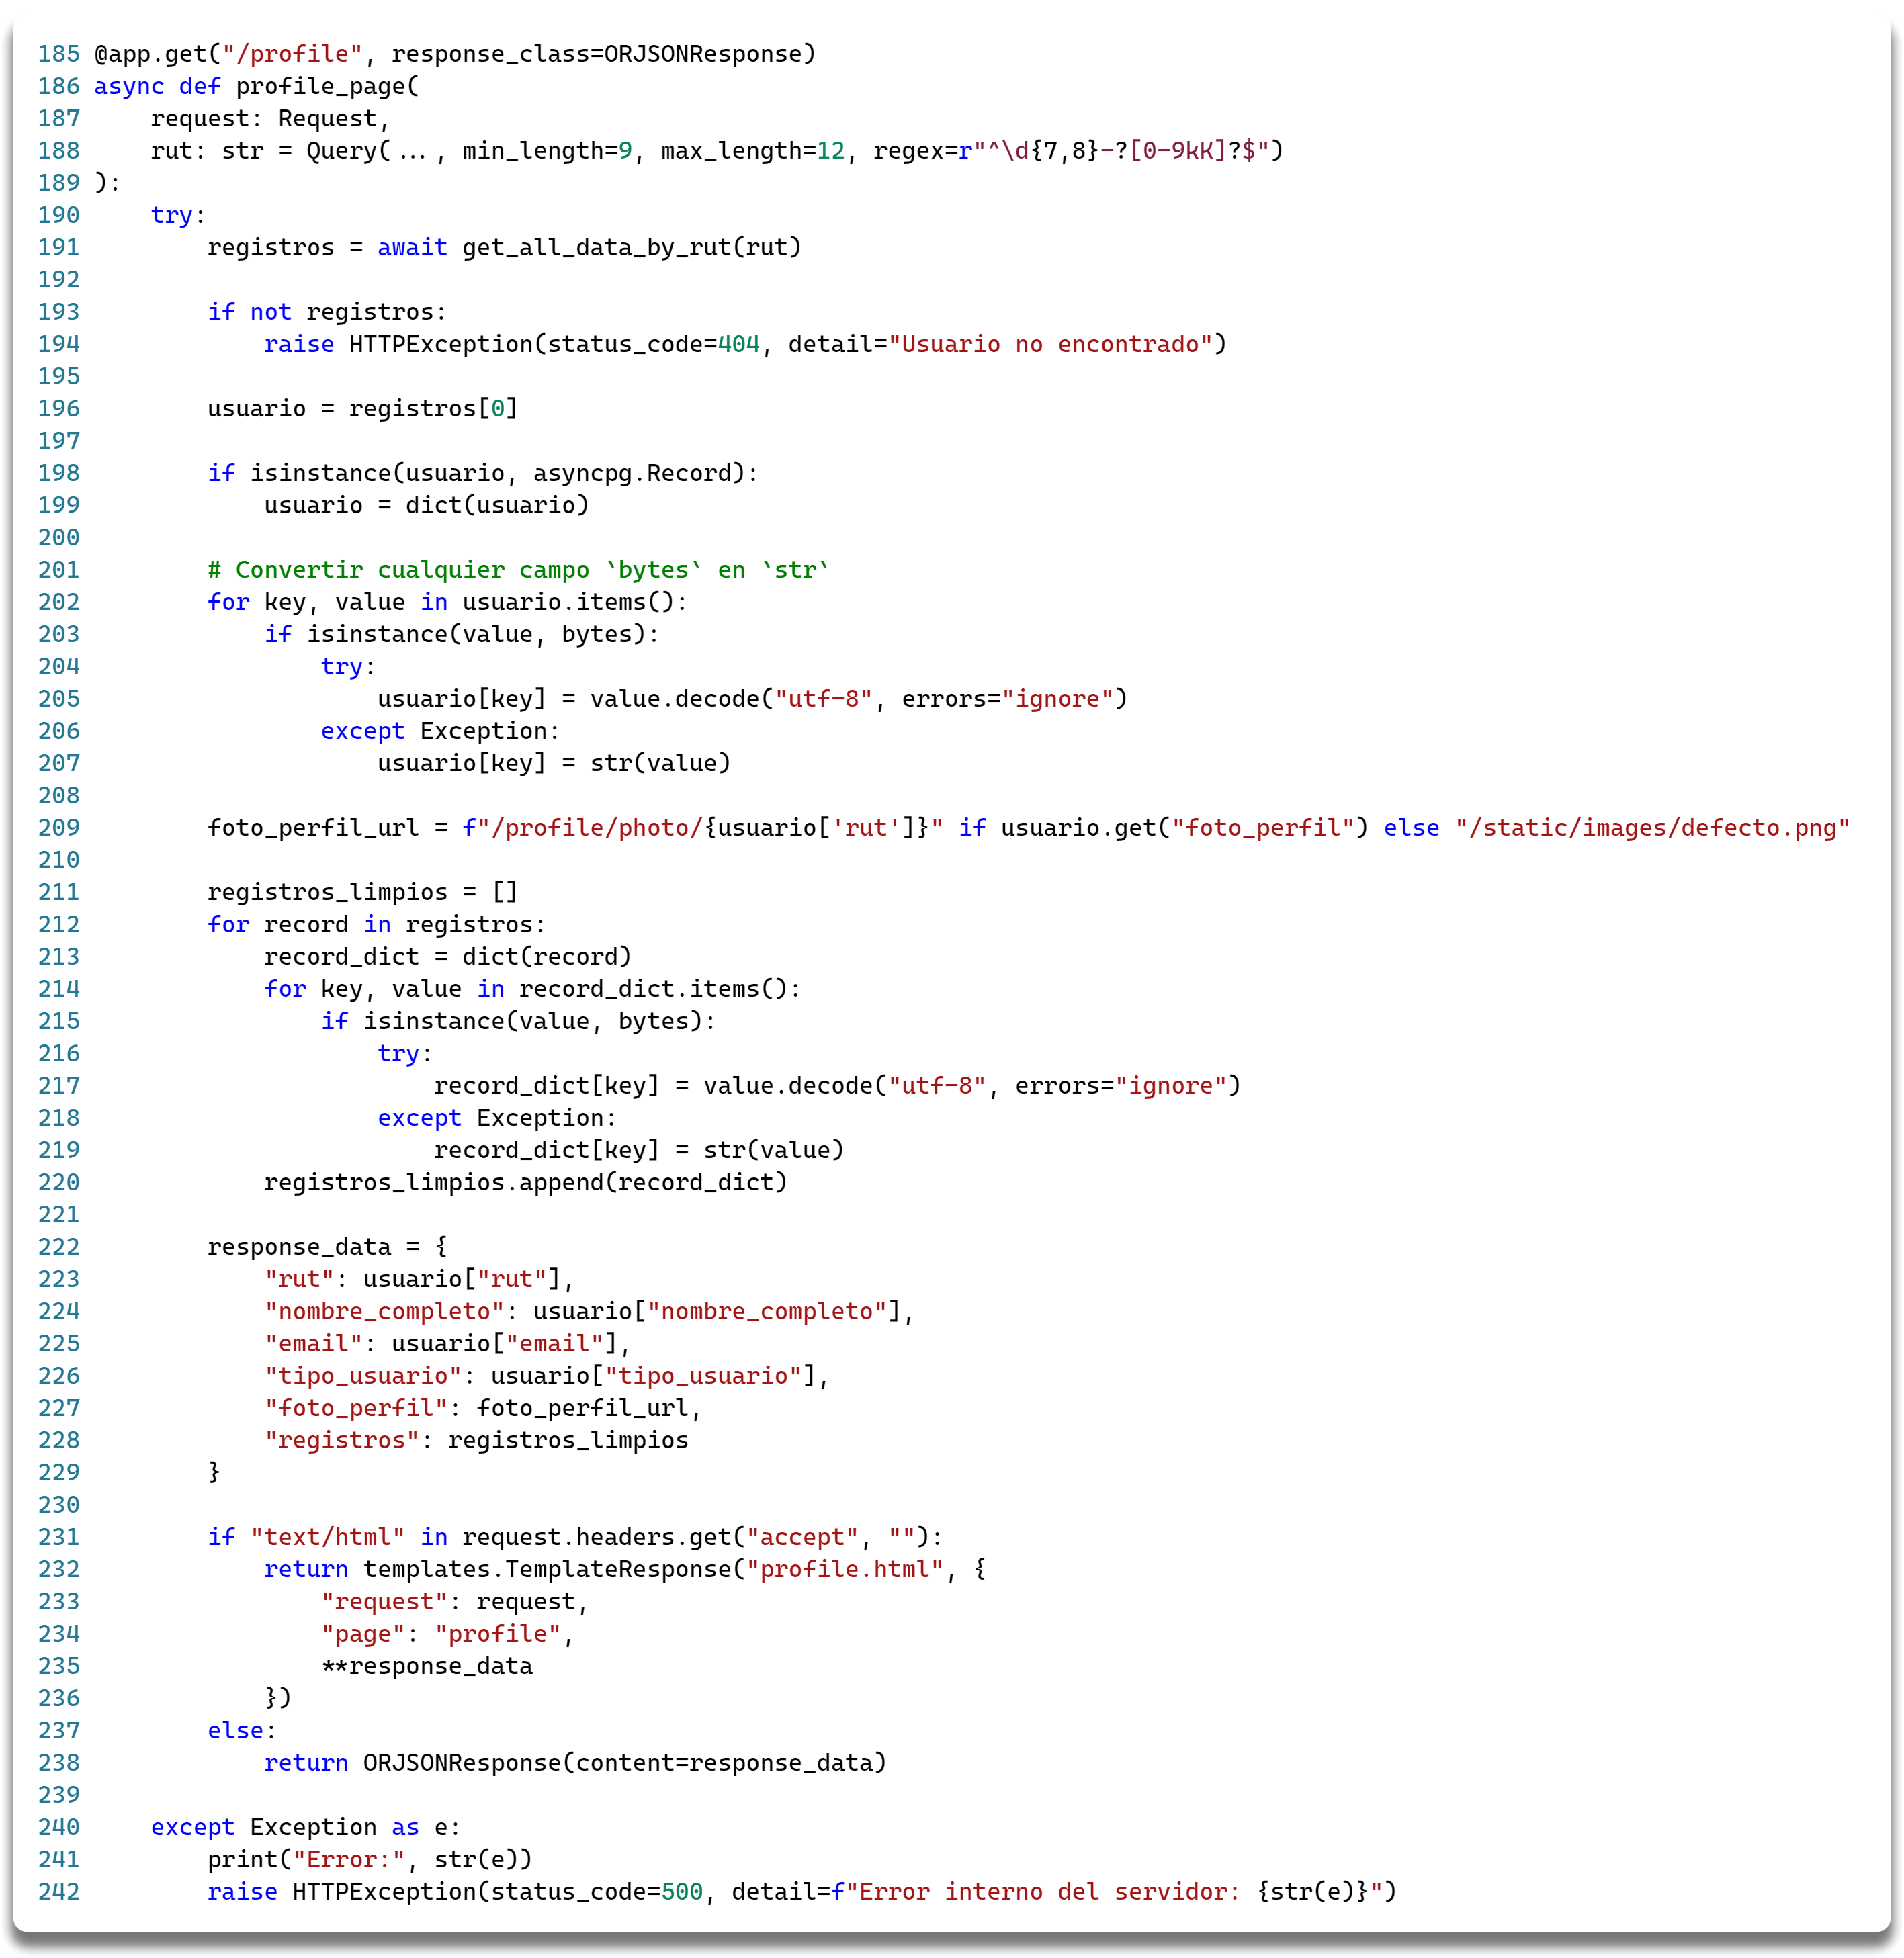
\includegraphics[width=\textwidth]{img/main10.png}
			            \caption{Archivo main.py Parte X}
			            \label{fig:main10}
		            \end{figure}
		            \newpage
		      \item Endpoint para iniciar sesion, el cual validara que el usuario exista y que las contraseña sea correcta. Luego le entregara un token JWT para poder ingresar a las páginas protegidas:
		            \begin{figure}[H]
			            \centering
			            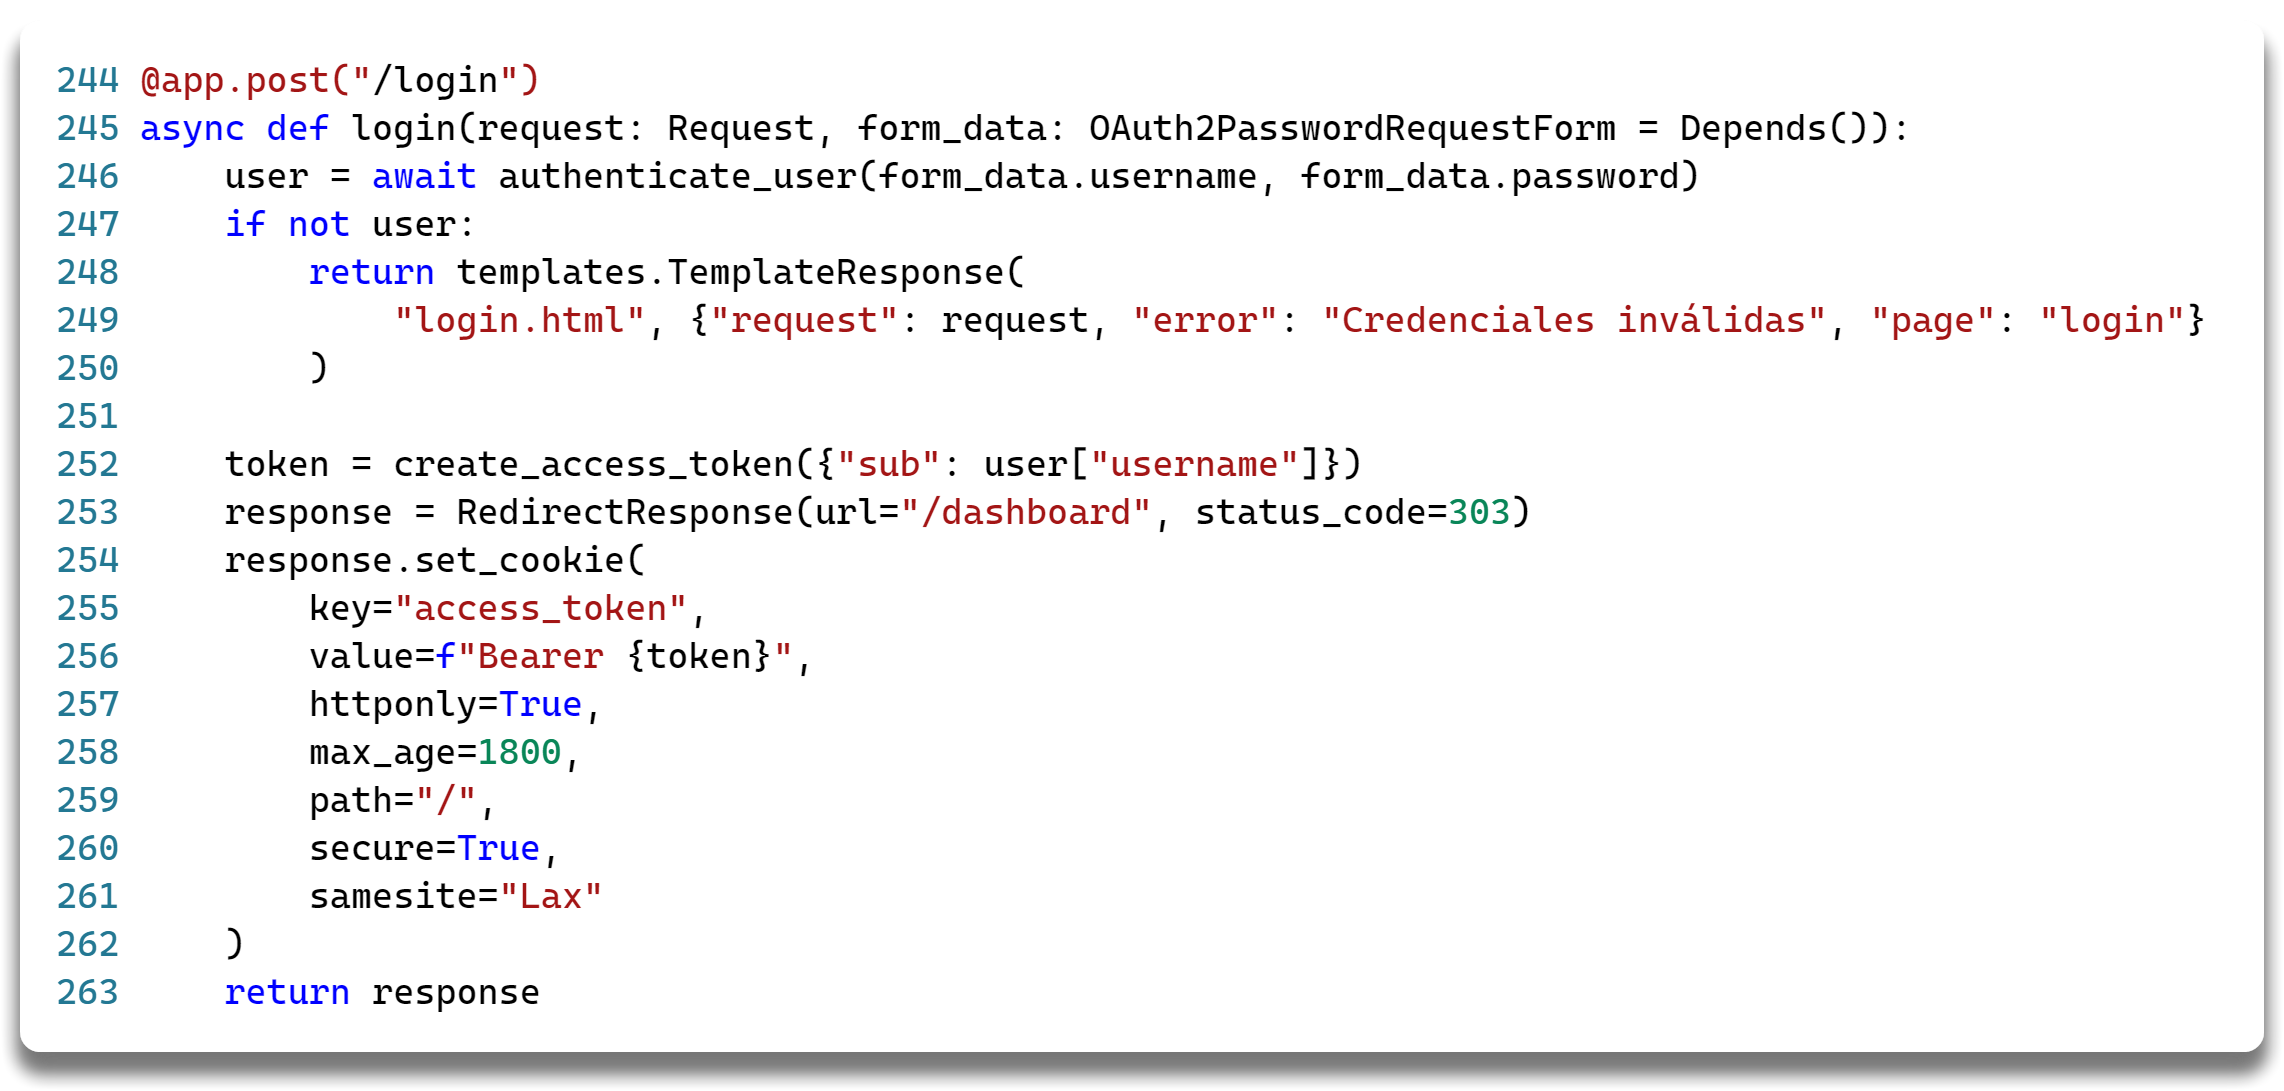
\includegraphics[width=\textwidth]{img/main11.png}
			            \caption{Archivo main.py Parte XI}
			            \label{fig:main11}
		            \end{figure}

		      \item Endpoint para cerrar sesion y eliminar el token de las cookies:
		            \begin{figure}[H]
			            \centering
			            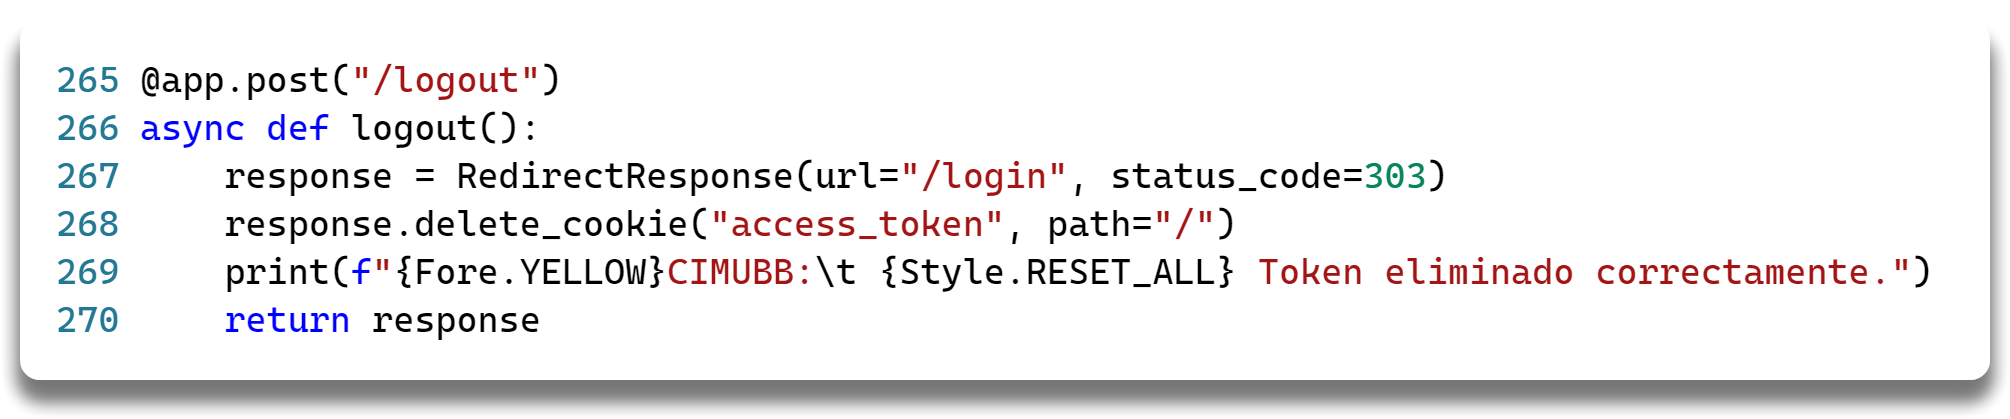
\includegraphics[width=\textwidth]{img/main12.png}
			            \caption{Archivo main.py Parte XII}
			            \label{fig:main12}
		            \end{figure}
		            \newpage
		      \item Endpoint para entregar los datos y notificaciones en el dashboard:
		            \begin{figure}[H]
			            \centering
			            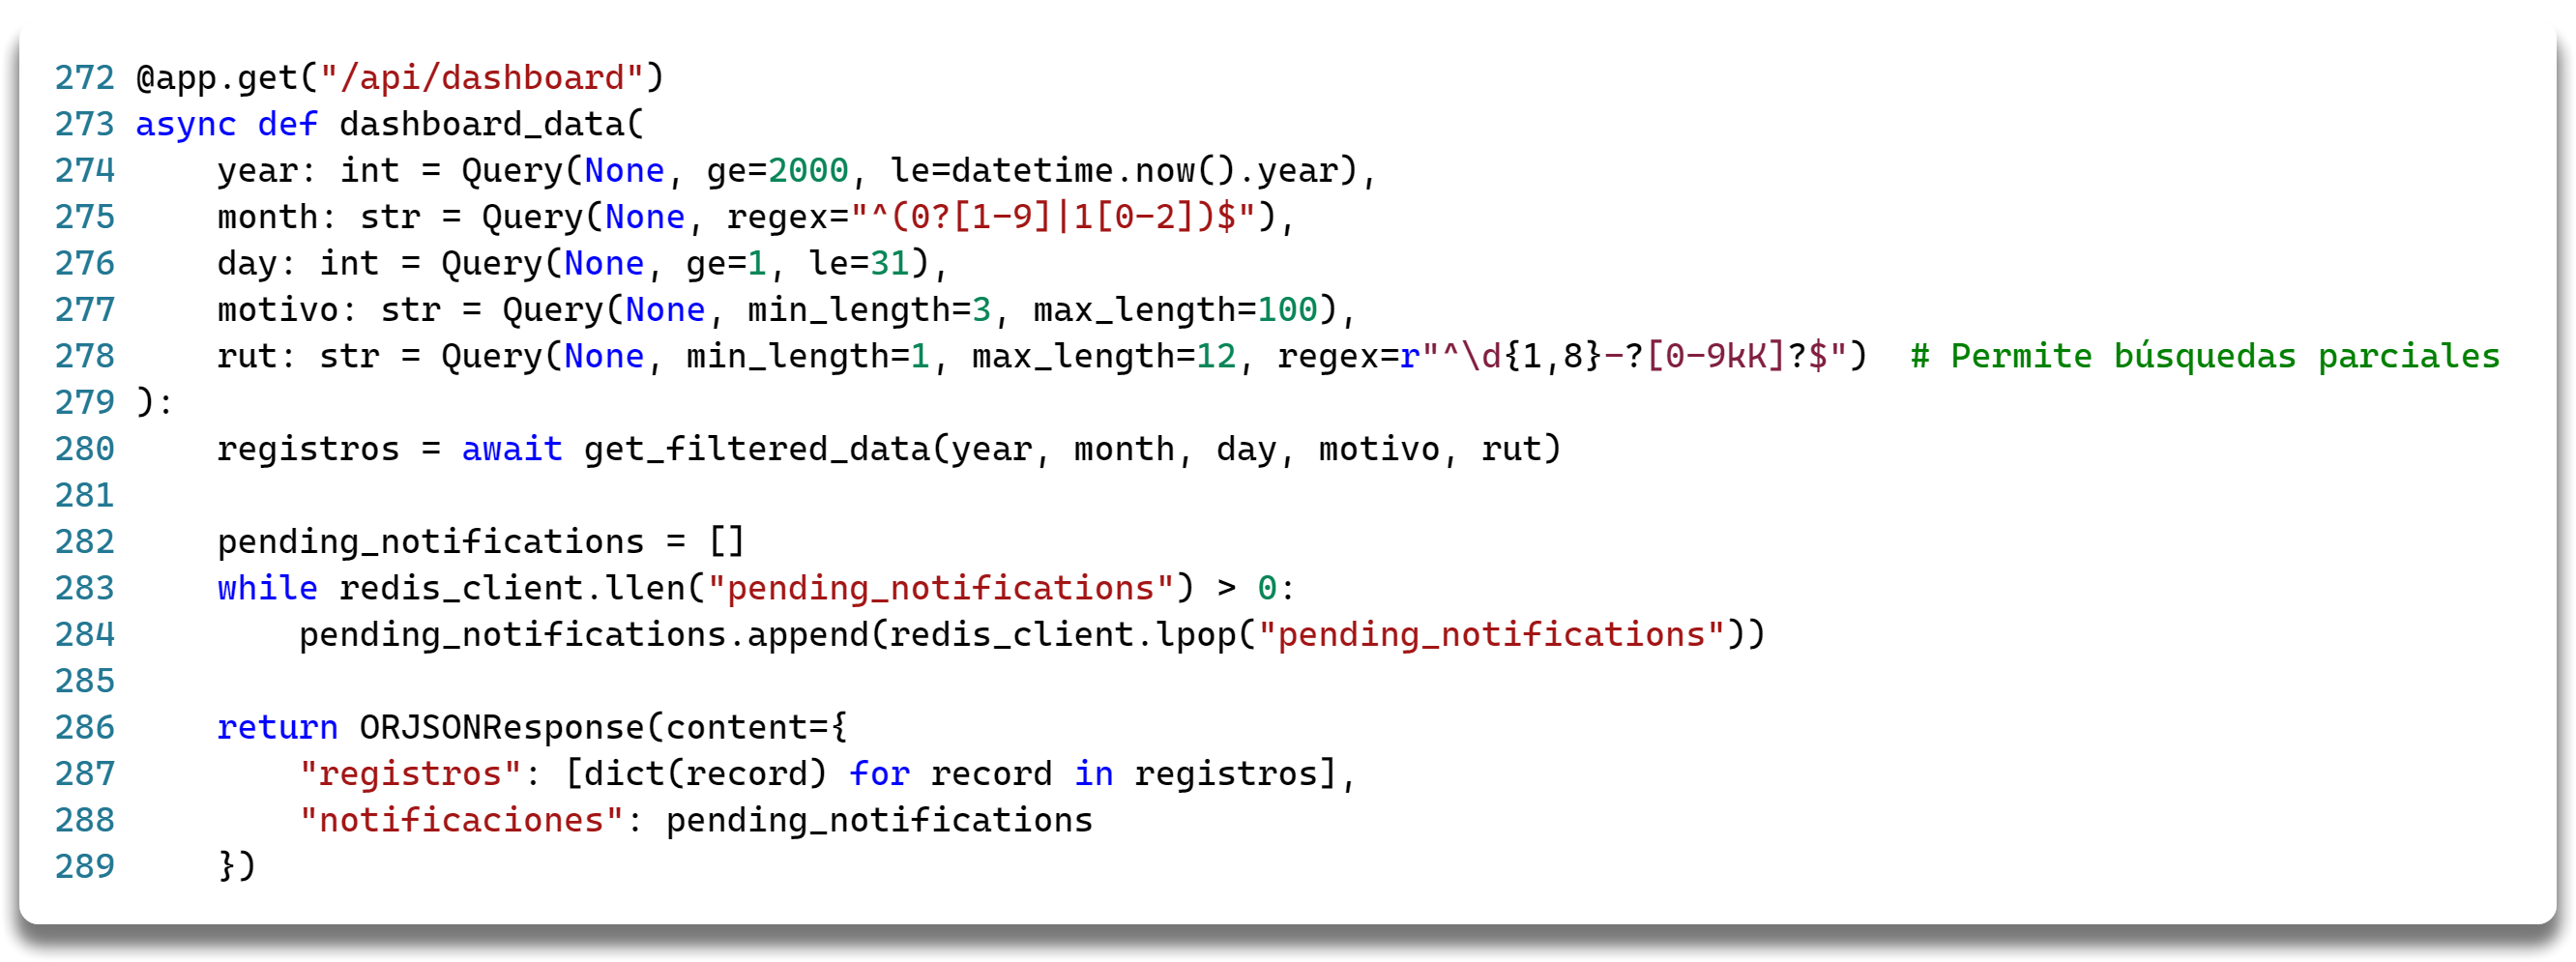
\includegraphics[width=\textwidth]{img/main13.png}
			            \caption{Archivo main.py Parte XIII}
			            \label{fig:main13}
		            \end{figure}
		      \item Endpoint para registrar un nuevo usuario desde la aplicación web:
		            \begin{figure}[H]
			            \centering
			            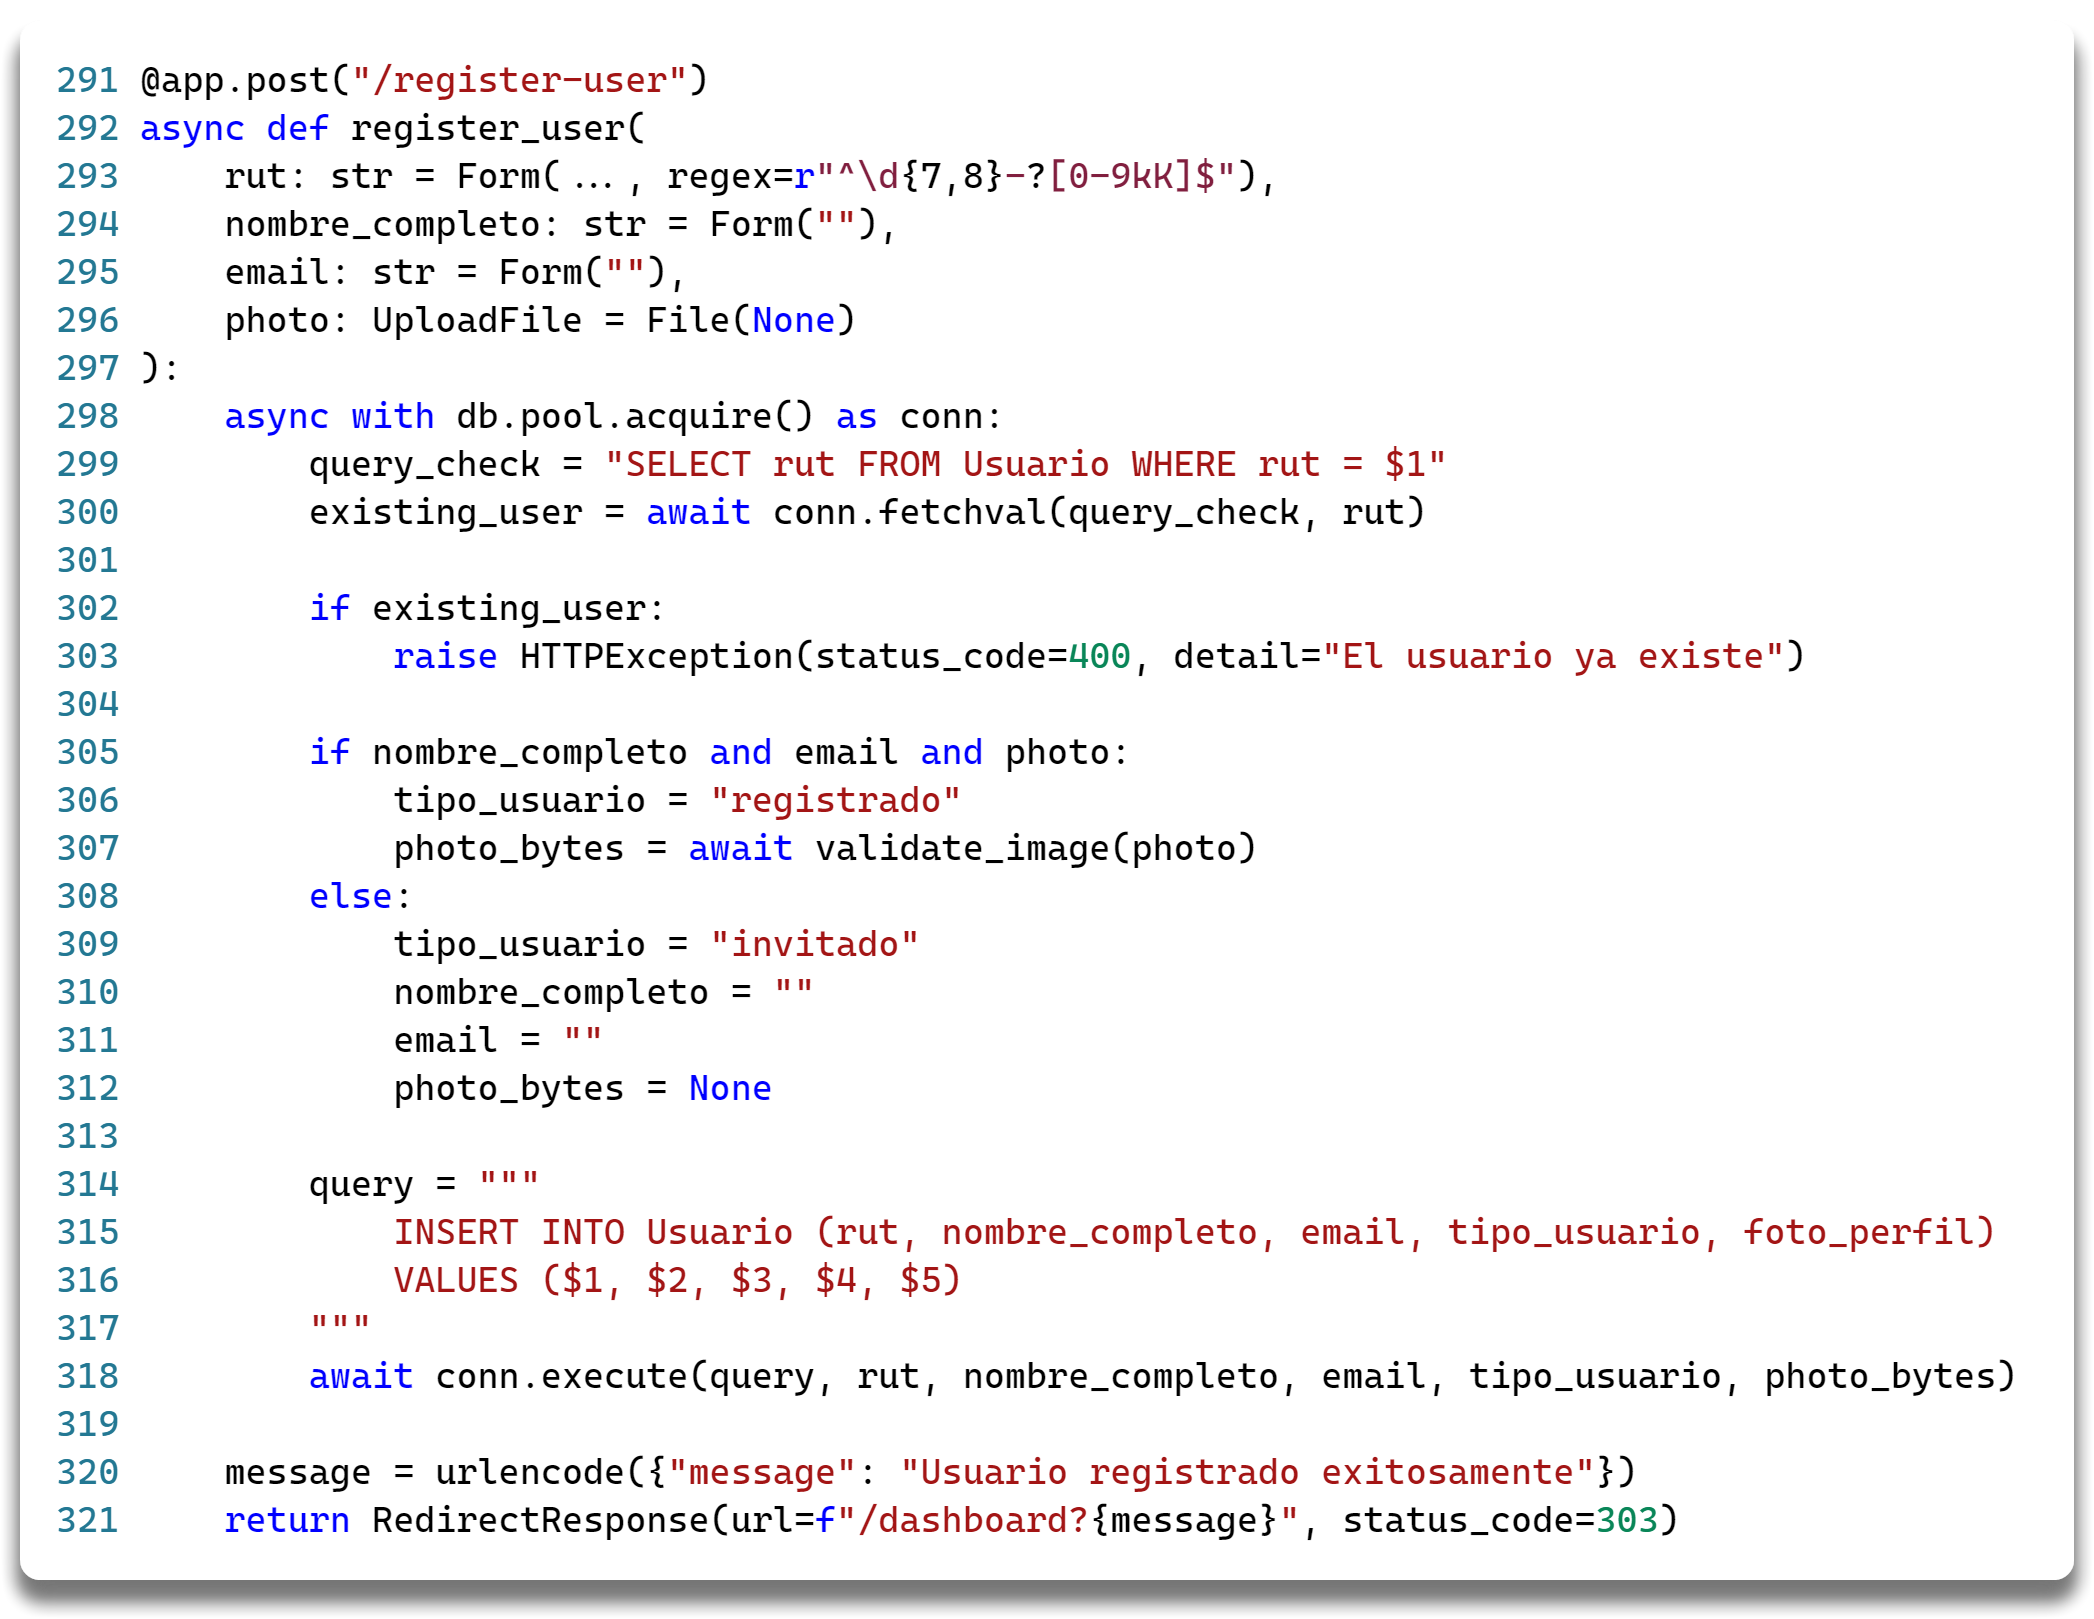
\includegraphics[width=\textwidth]{img/main14.png}
			            \caption{Archivo main.py Parte XIV}
			            \label{fig:main14}
		            \end{figure}
		            \newpage
		      \item Endpoint para registrar un nuevo administrador (LOGIN) desde la aplicación web:
		            \begin{figure}[H]
			            \centering
			            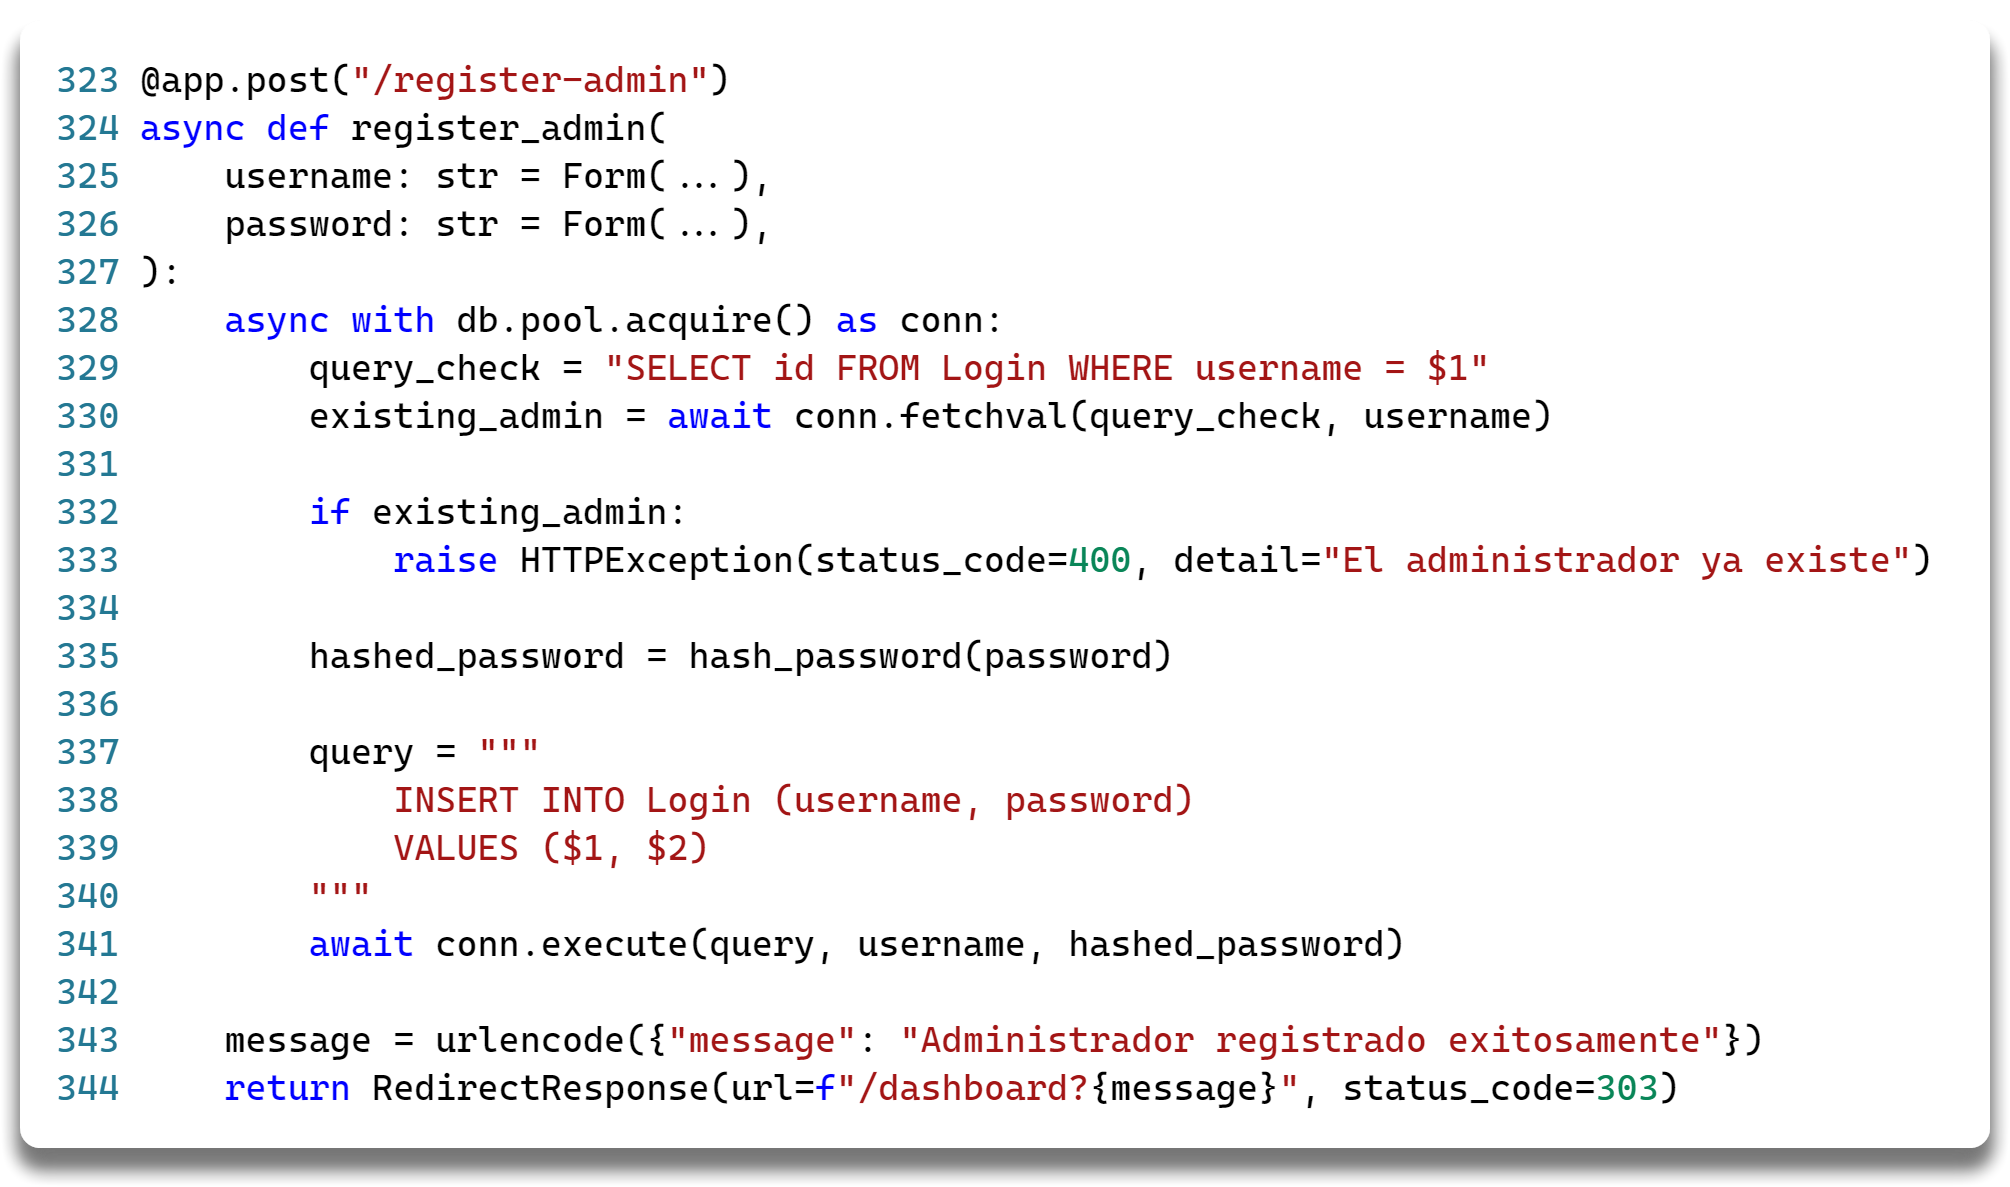
\includegraphics[width=\textwidth]{img/main15.png}
			            \caption{Archivo main.py Parte XV}
			            \label{fig:main15}
		            \end{figure}

		      \item Endpoint para agregar un nuevo WebSocket a la escucha, en el que se entregaran las notificaciones que se encuentren en cola y evitar el t\'ermino de la comunicación:
		            \begin{figure}[H]
			            \centering
			            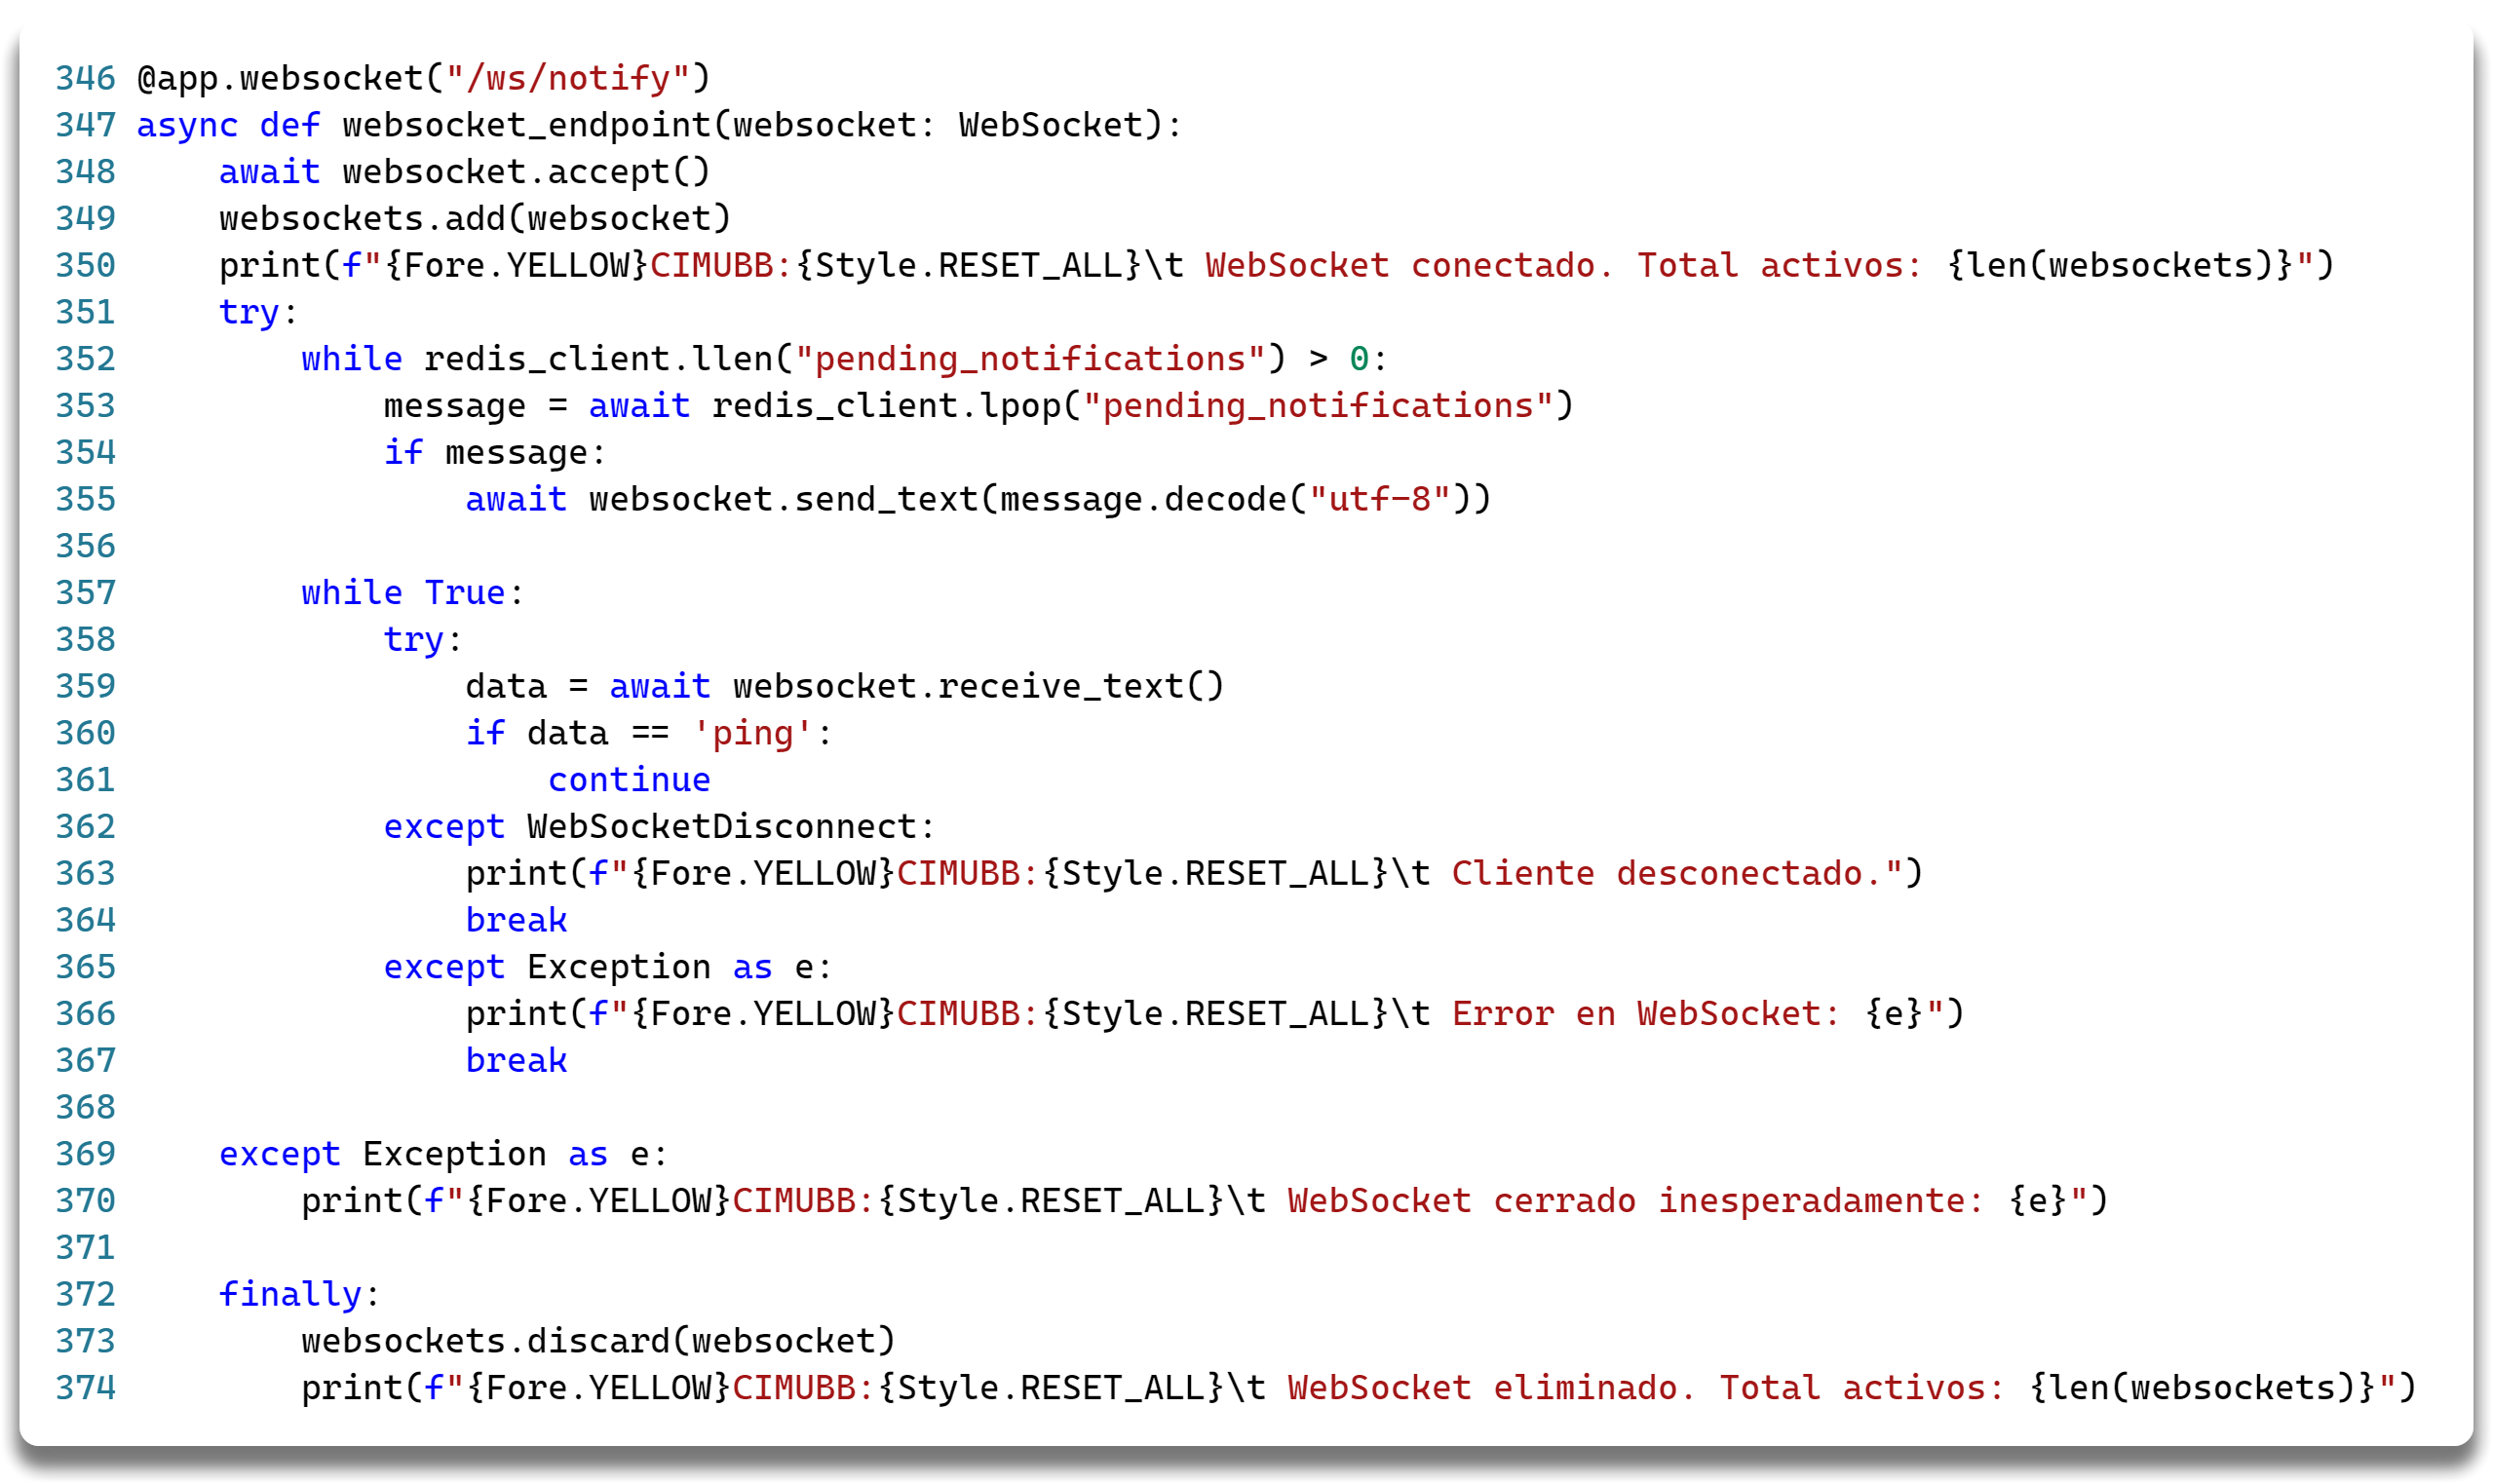
\includegraphics[width=\textwidth]{img/main16.png}
			            \caption{Archivo main.py Parte XVI}
			            \label{fig:main16}
		            \end{figure}

		      \item Excepci\'on que se encarga de mejorar el envi\'o de errores para la facil detección del campo que puede estar generando problemas:
		            \begin{figure}[H]
			            \centering
			            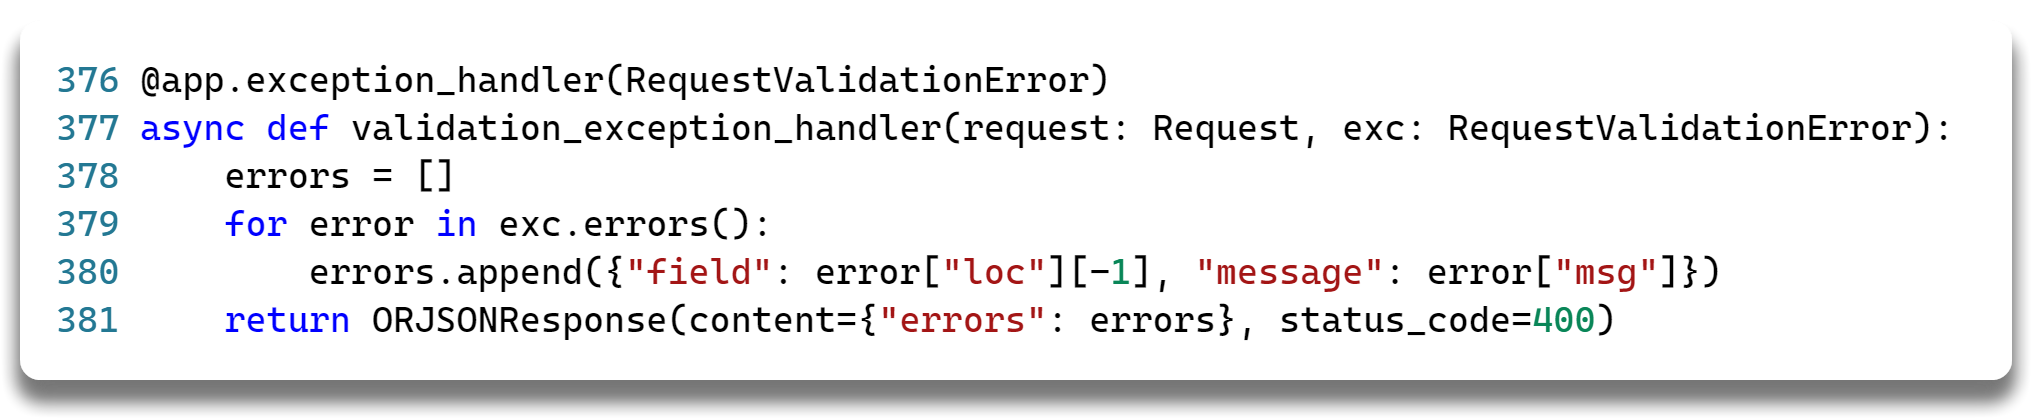
\includegraphics[width=\textwidth]{img/main17.png}
			            \caption{Archivo main.py Parte XVII}
			            \label{fig:main17}
		            \end{figure}
	      \end{enumerate}

	\item \textbf{base.html}:
	      \begin{enumerate}
		      \item En resumen es la base para el renderizado, se utiliza jinja2 el cual mediante definici\'on de bloques se puede ir ensamblando html m\'as peque\~nos, en esta base agregamos scripts y los iconos generales, reconocemos la etiqueta de la pagina y agregamos los estilos especificos:
		            \begin{figure}[H]
			            \centering
			            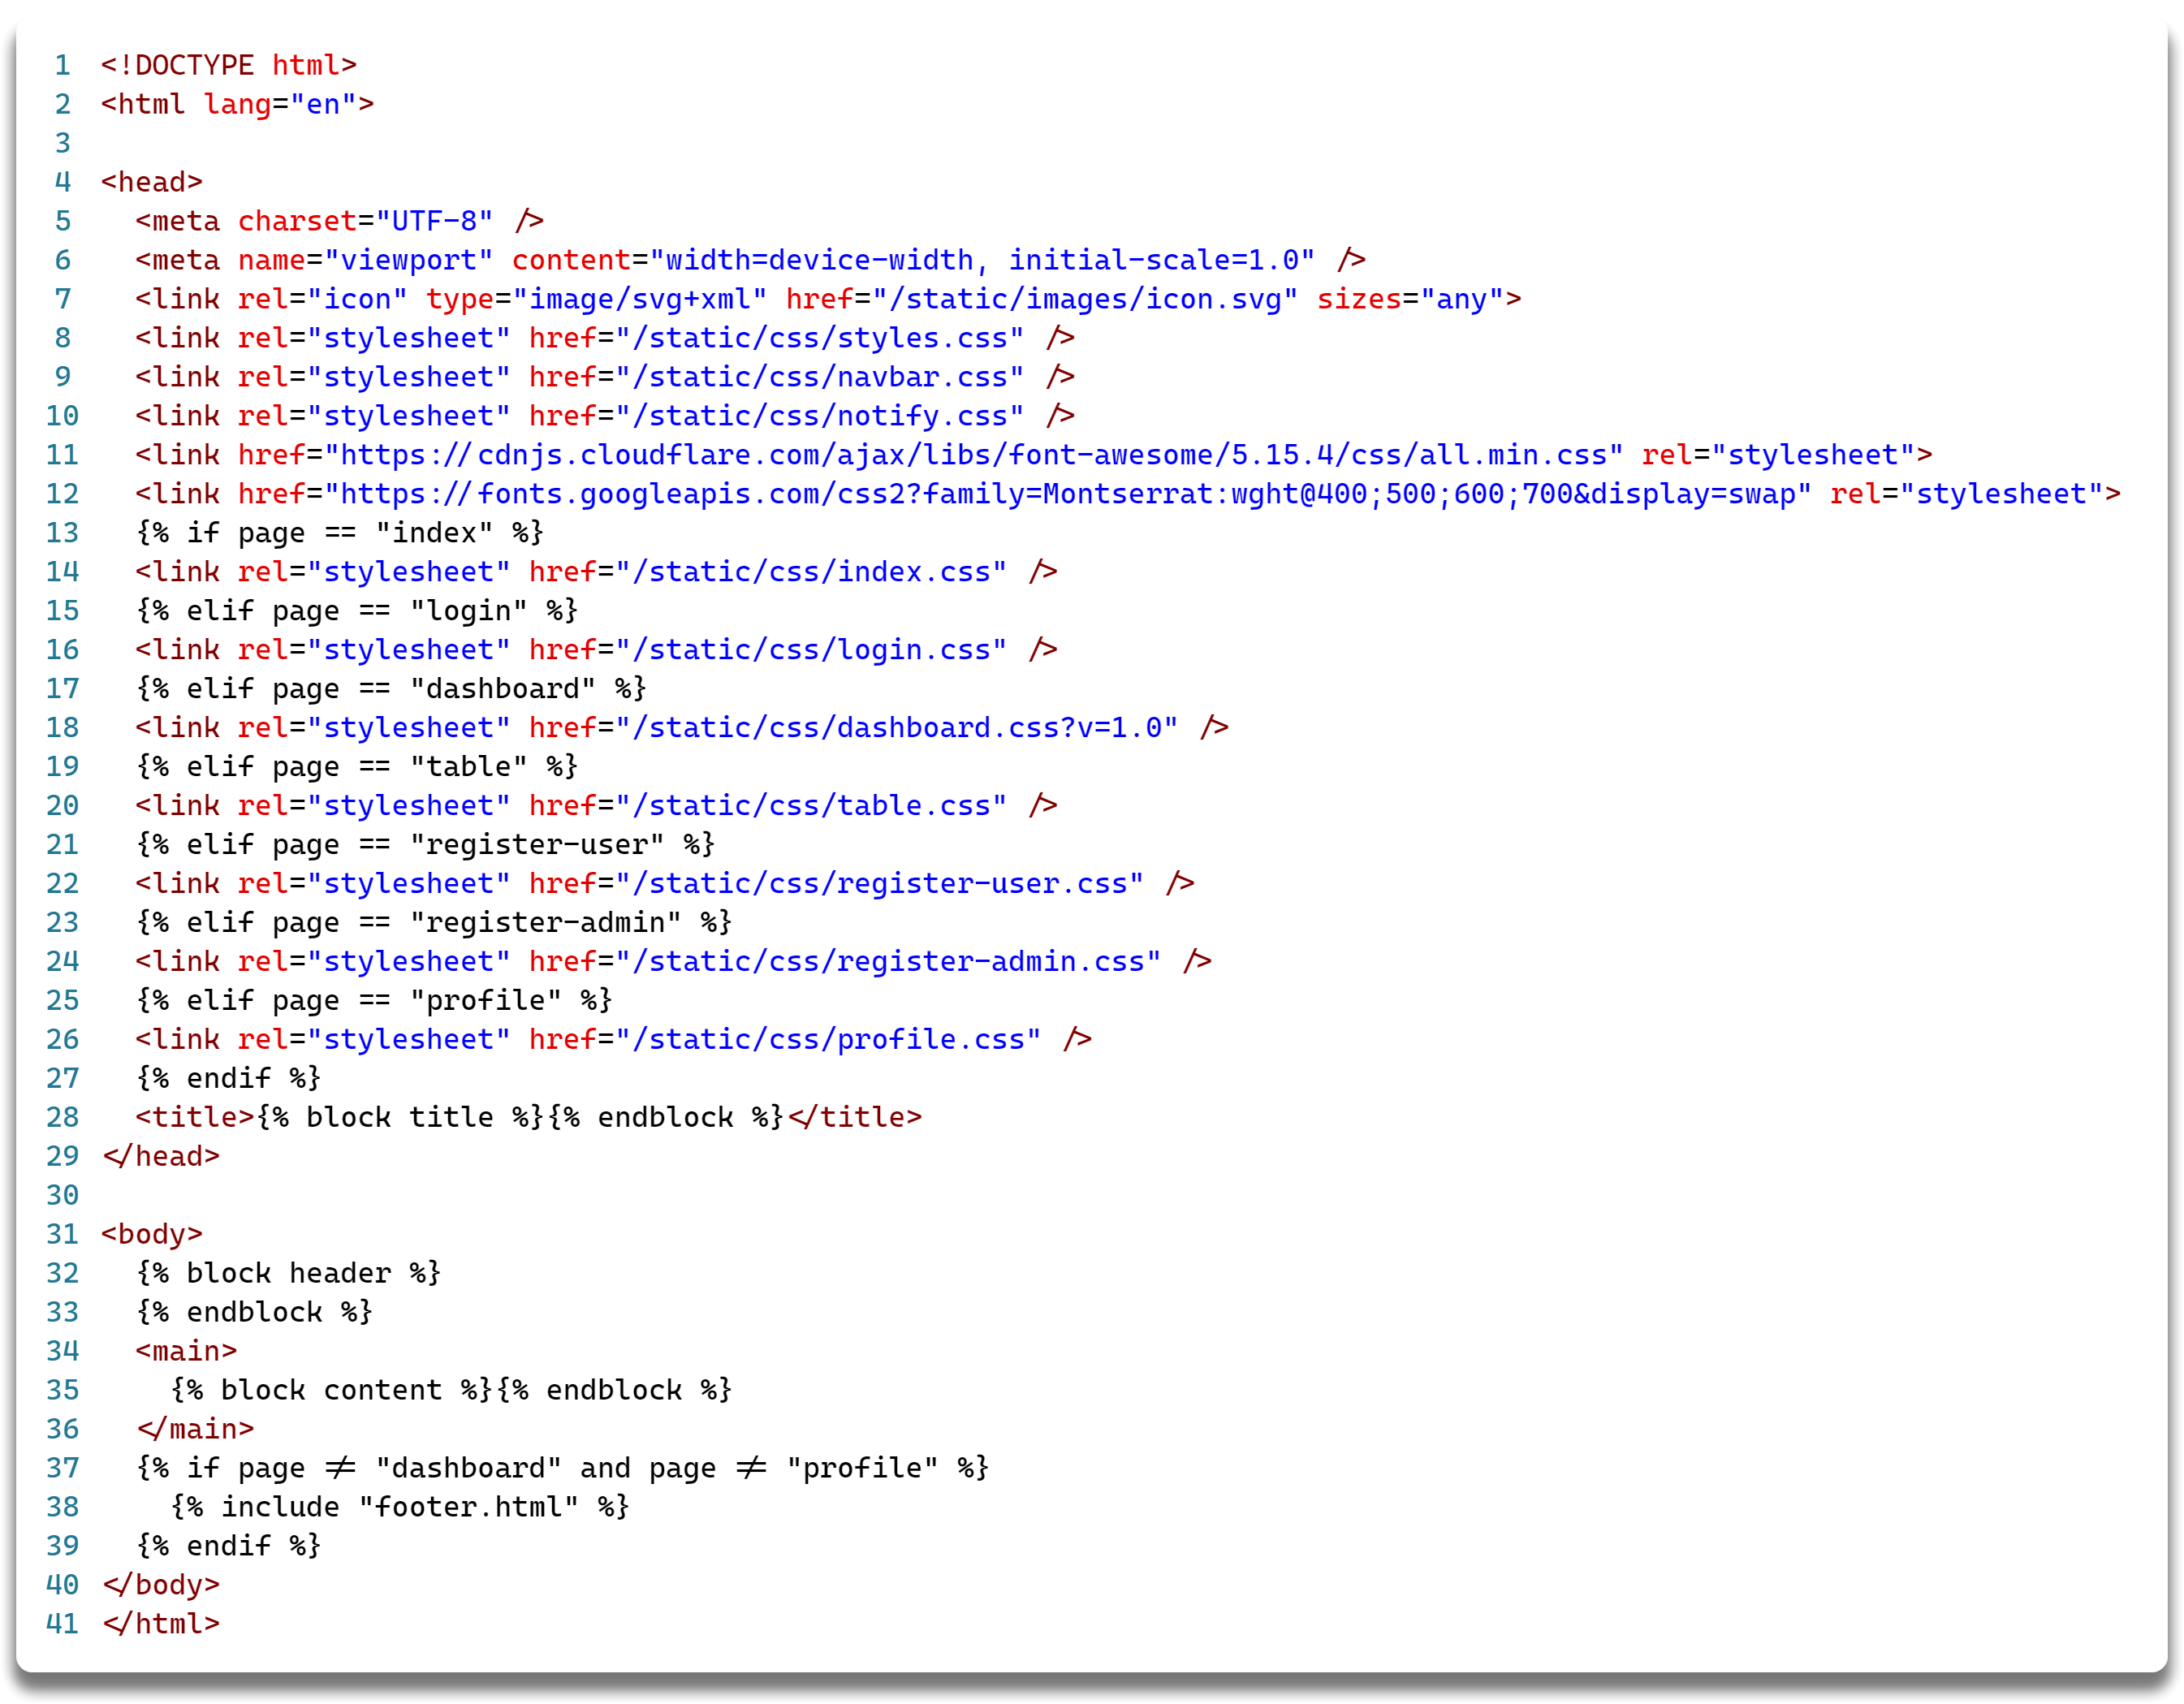
\includegraphics[width=\textwidth]{img/baseHTML.png}
			            \caption{Archivo base.html}
			            \label{fig:baseHTML}
		            \end{figure}
	      \end{enumerate}
	      \newpage
	\item \textbf{navbar.html}:
	      \begin{enumerate}
		      \item Este componente contiene las referencias a las secciones de la aplicación web:
		            \begin{figure}[H]
			            \centering
			            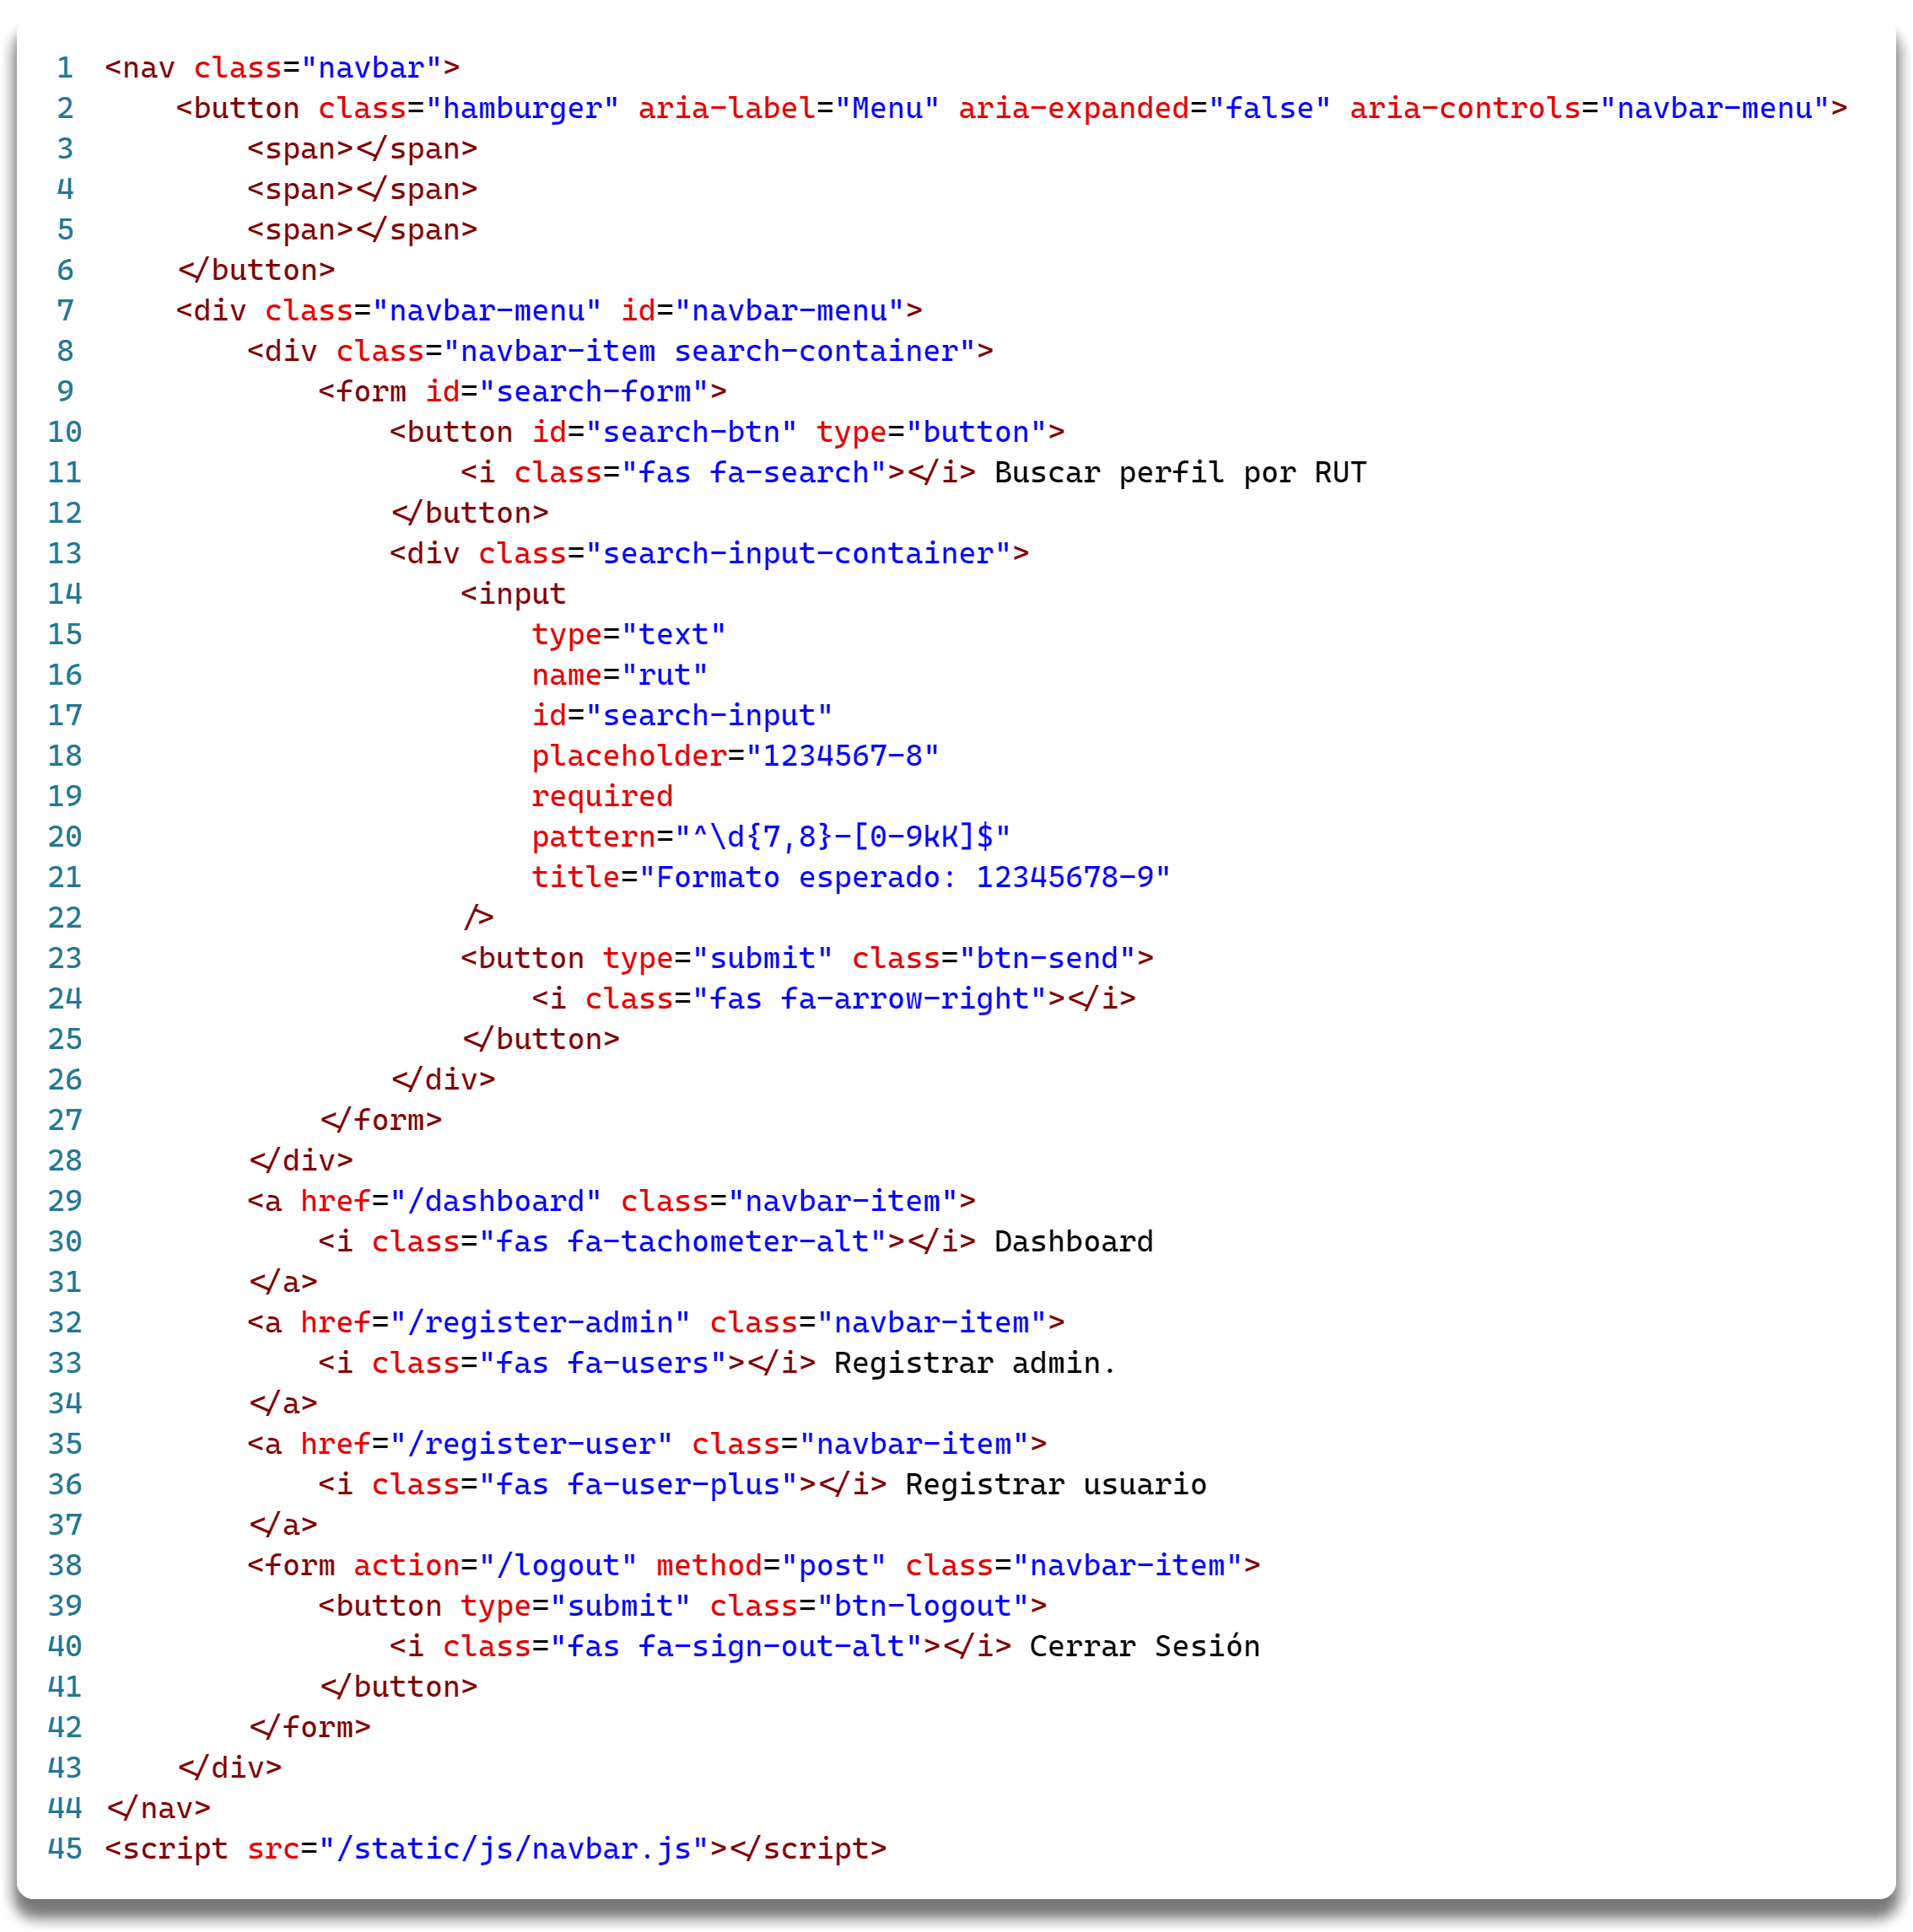
\includegraphics[width=\textwidth]{img/navbarHTML.png}
			            \caption{Archivo navbar.html}
			            \label{fig:navbarHTML}
		            \end{figure}
	      \end{enumerate}
	      \newpage
	\item \textbf{navbar.js}:
	      \begin{enumerate}
		      \item Este c\'odigo contiene la función que activa la visualización del navbar modificando su clase y por lo tanto su CSS, adem\'as de la l\'ogica para hacer funcionar el boton que busca un rut especifico:
		            \begin{figure}[H]
			            \centering
			            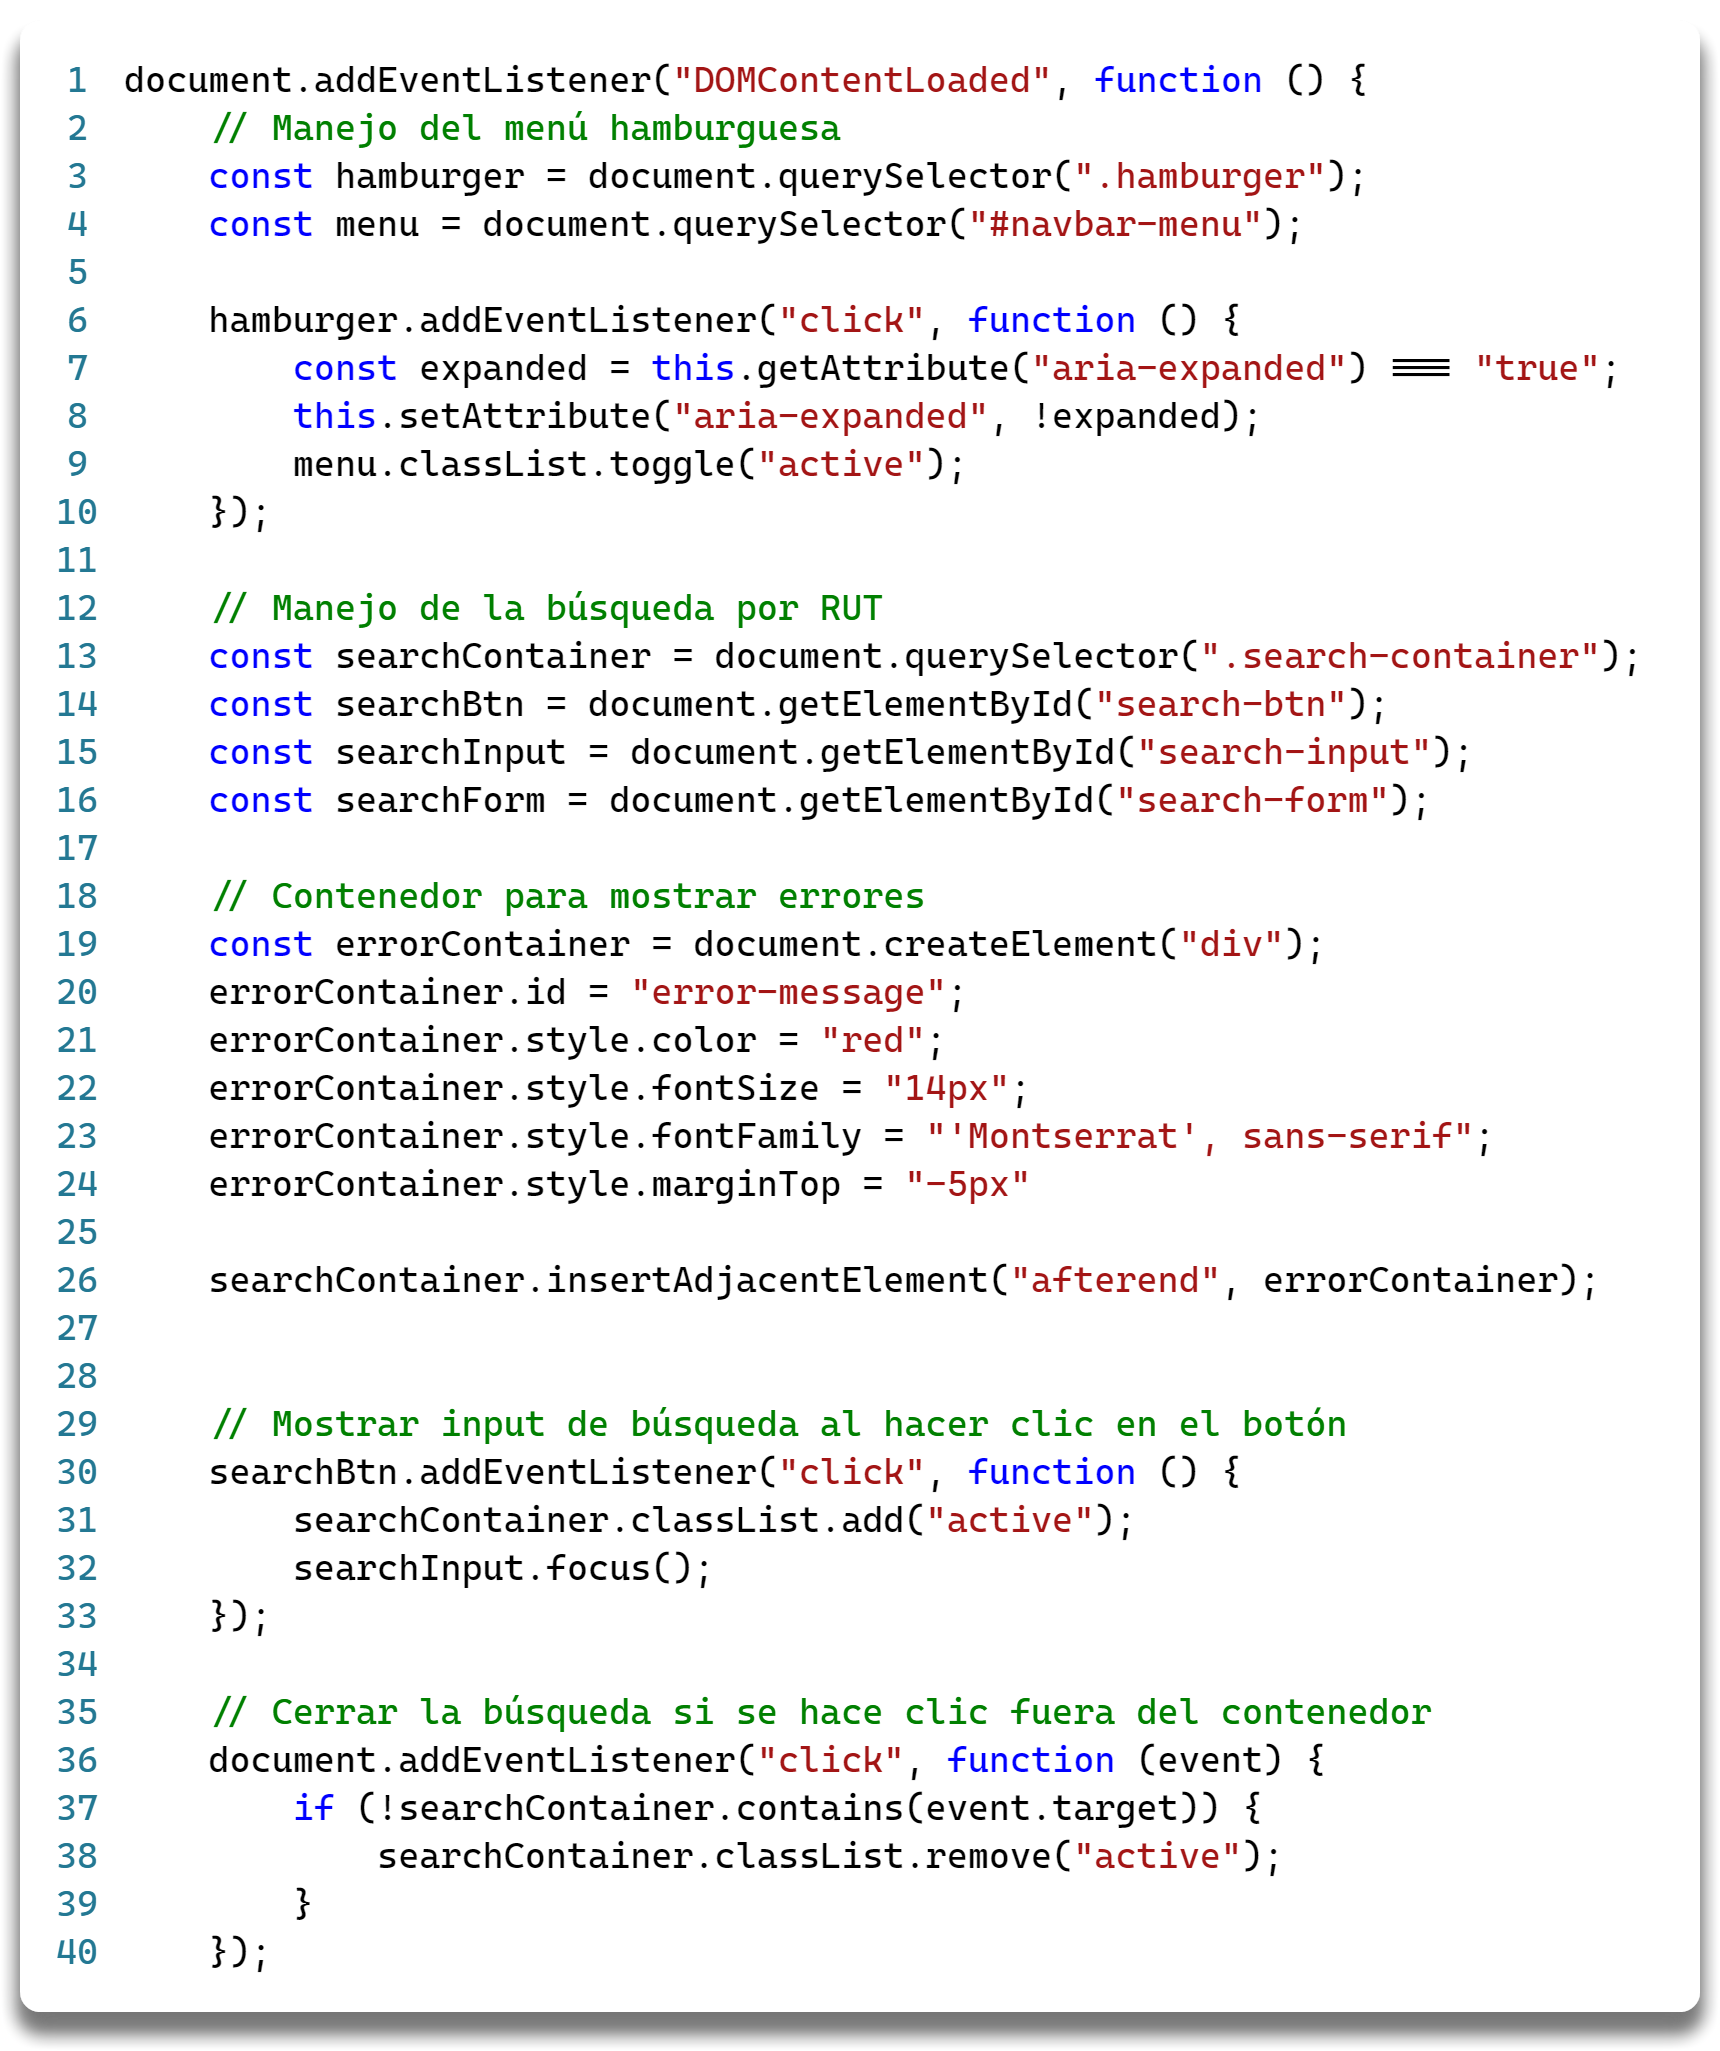
\includegraphics[width=\textwidth]{img/navbarJS1.png}
			            \caption{Archivo navbar.js Parte I}
			            \label{fig:navbarJS1}
		            \end{figure}
		            \newpage
		      \item Este c\'odigo maneja las validaciones del backend para mostrar si el rut existe o si no cumple con el formato:
		            \begin{figure}[H]
			            \centering
			            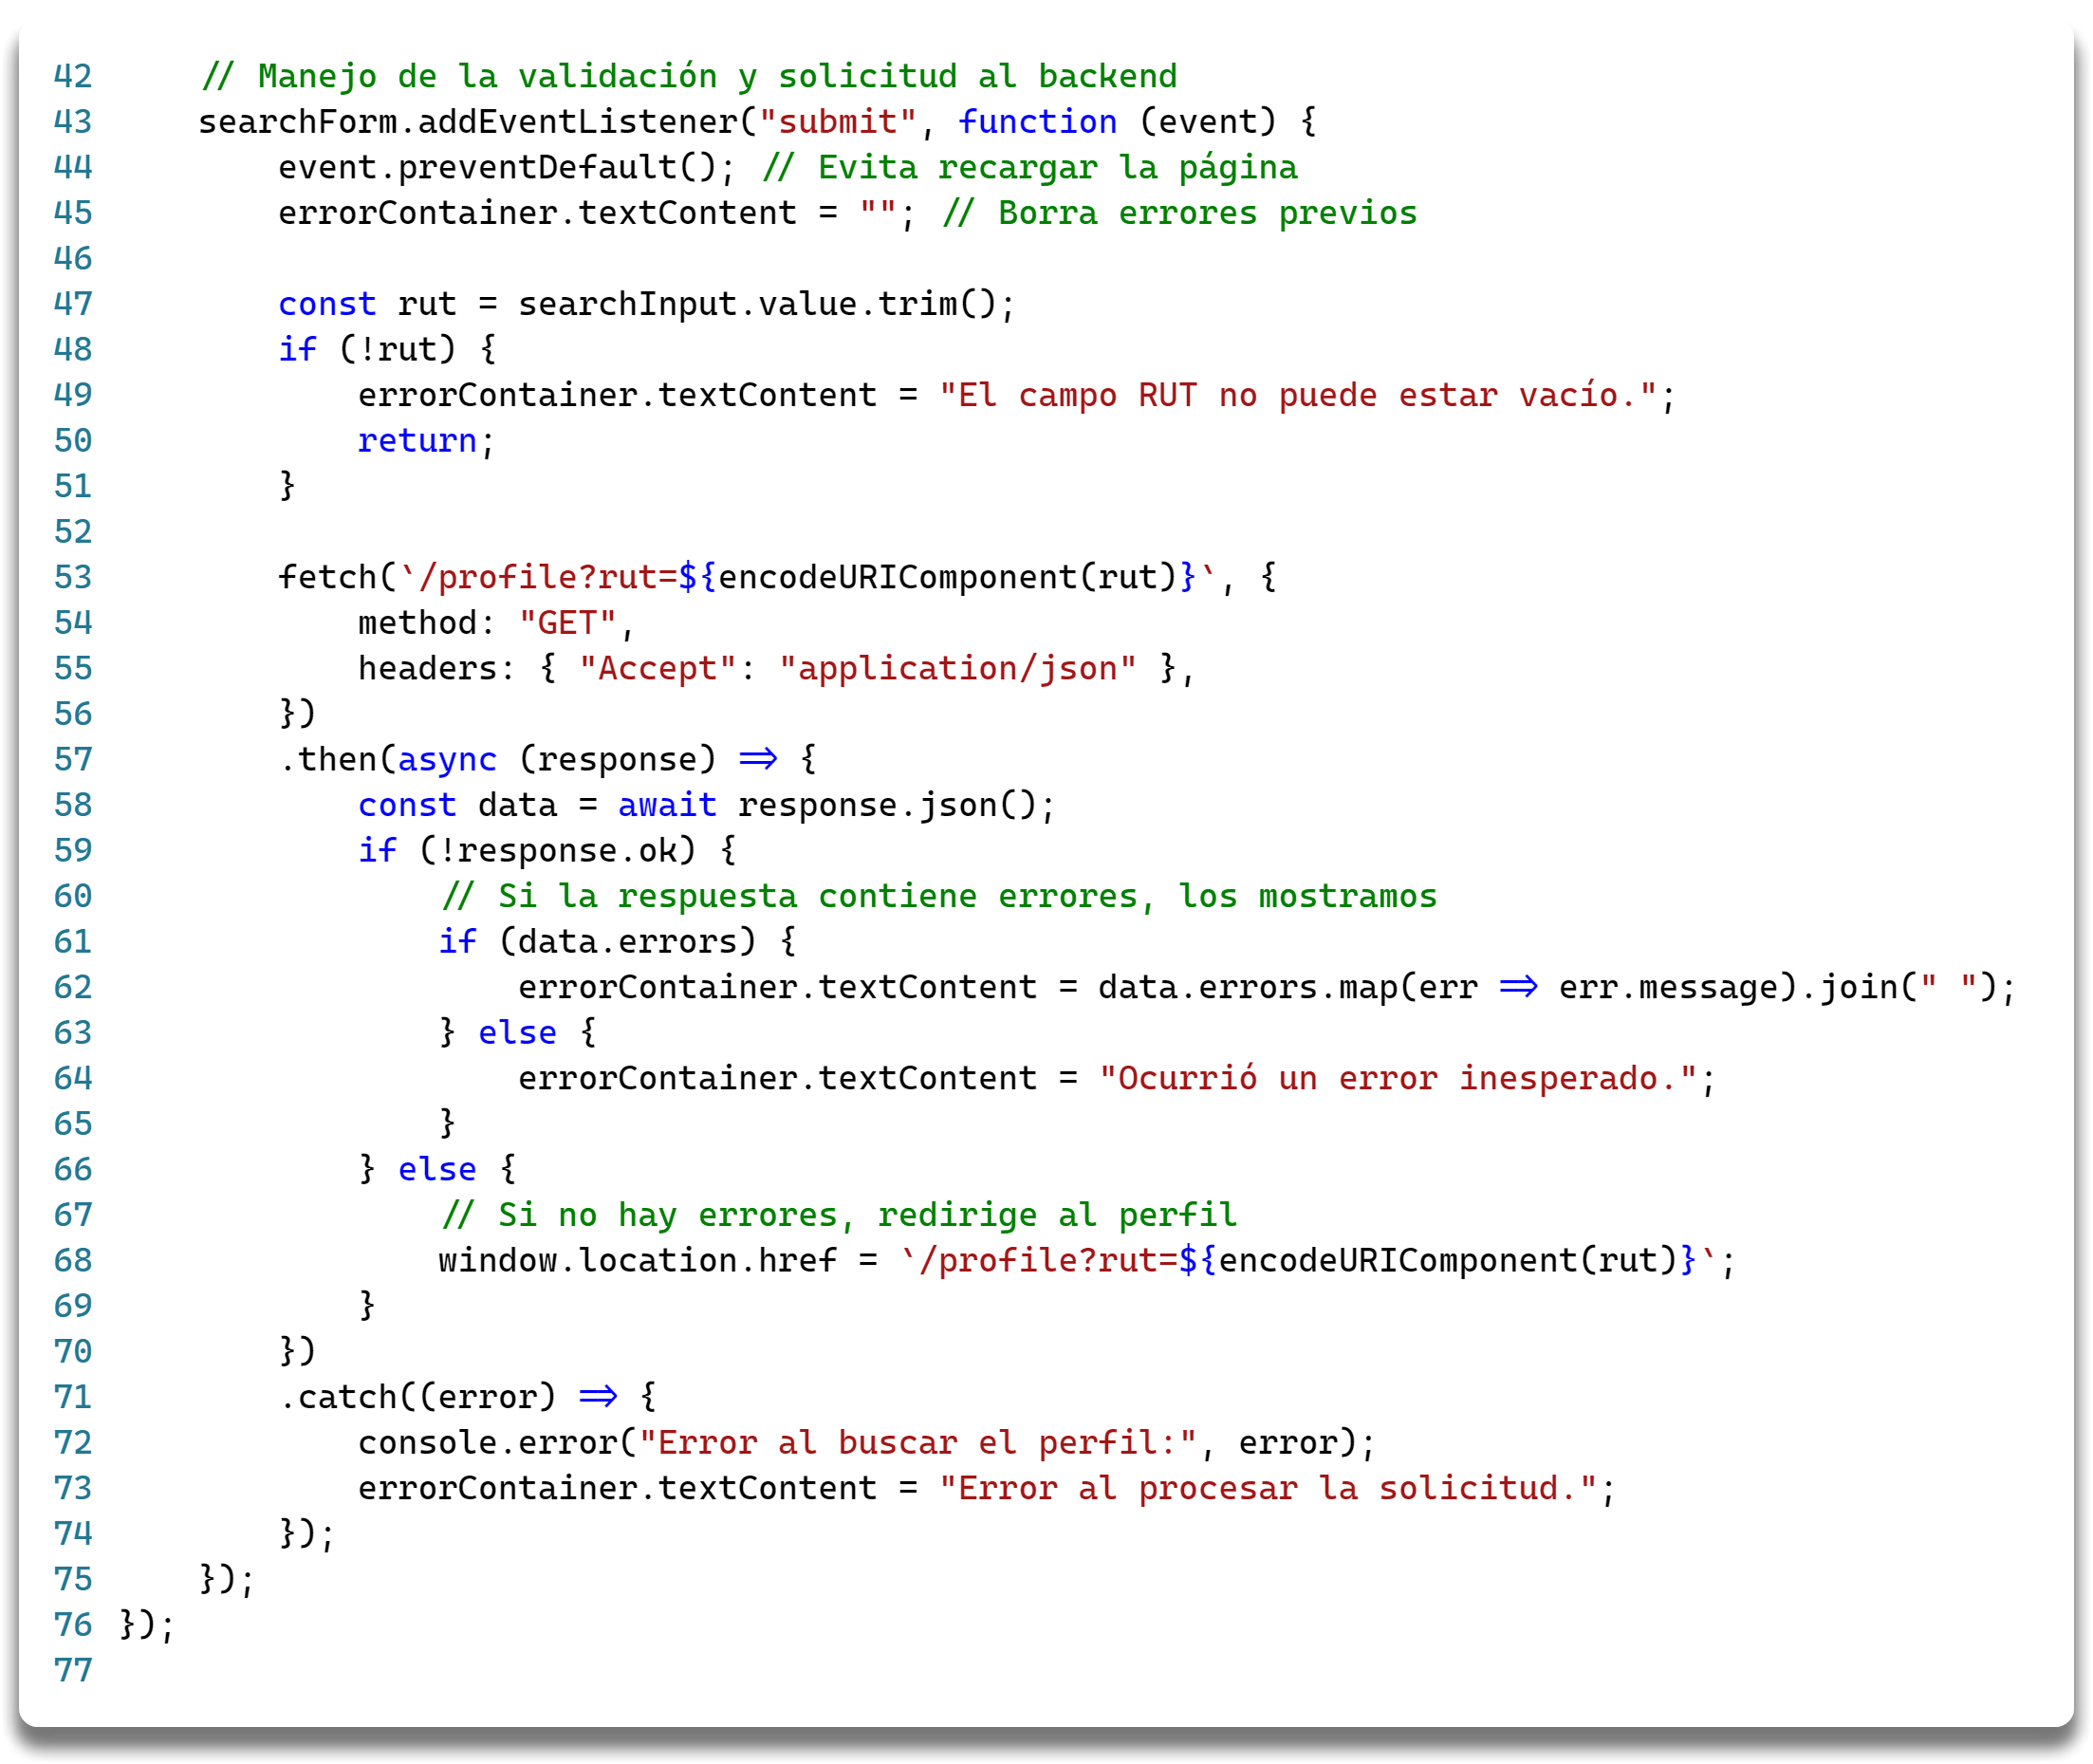
\includegraphics[width=\textwidth]{img/navbarJS2.png}
			            \caption{Archivo navbar.js Parte II}
			            \label{fig:navbarJS2}
		            \end{figure}
	      \end{enumerate}

	\item \textbf{dashboard.html}:
	      \begin{enumerate}
		      \item Se le dice a jinja2 que se utiliza base.html, se le agrega un titulo a la p\'agina y se agregan los componentes navbar y notify:
		            \begin{figure}[H]
			            \centering
			            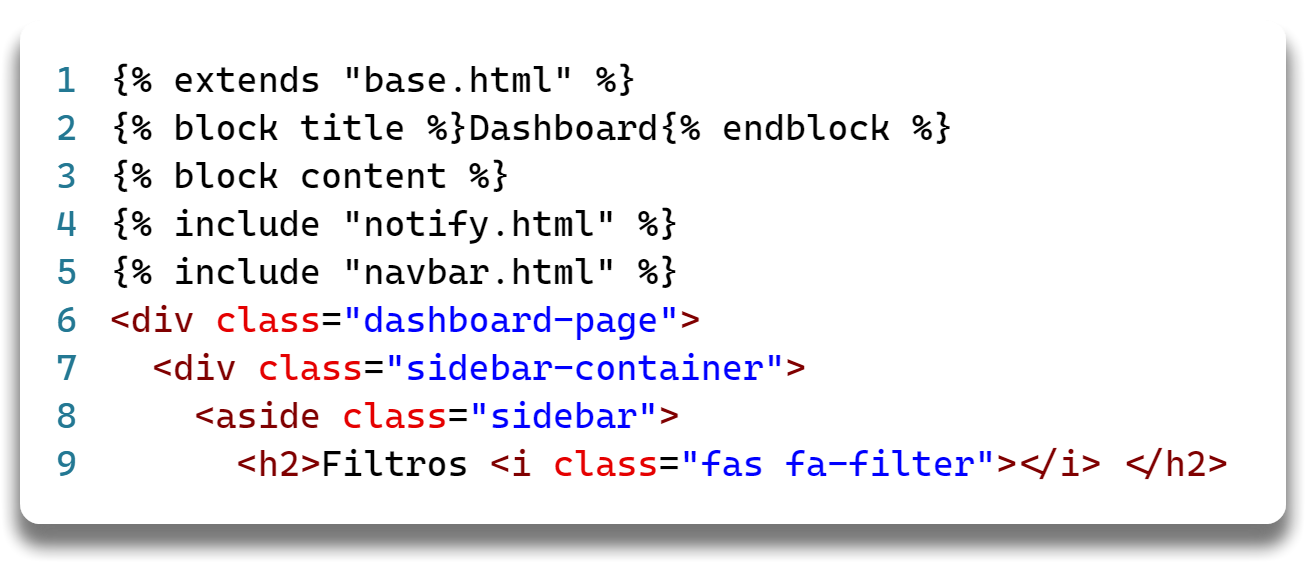
\includegraphics[width=0.6\textwidth]{img/dashboardHTML1.png}
			            \caption{Archivo dashboard.html Parte I}
			            \label{fig:dashboardHTML1}
		            \end{figure}
		      \item Se pone un filtro para el año:
		            \begin{figure}[H]
			            \centering
			            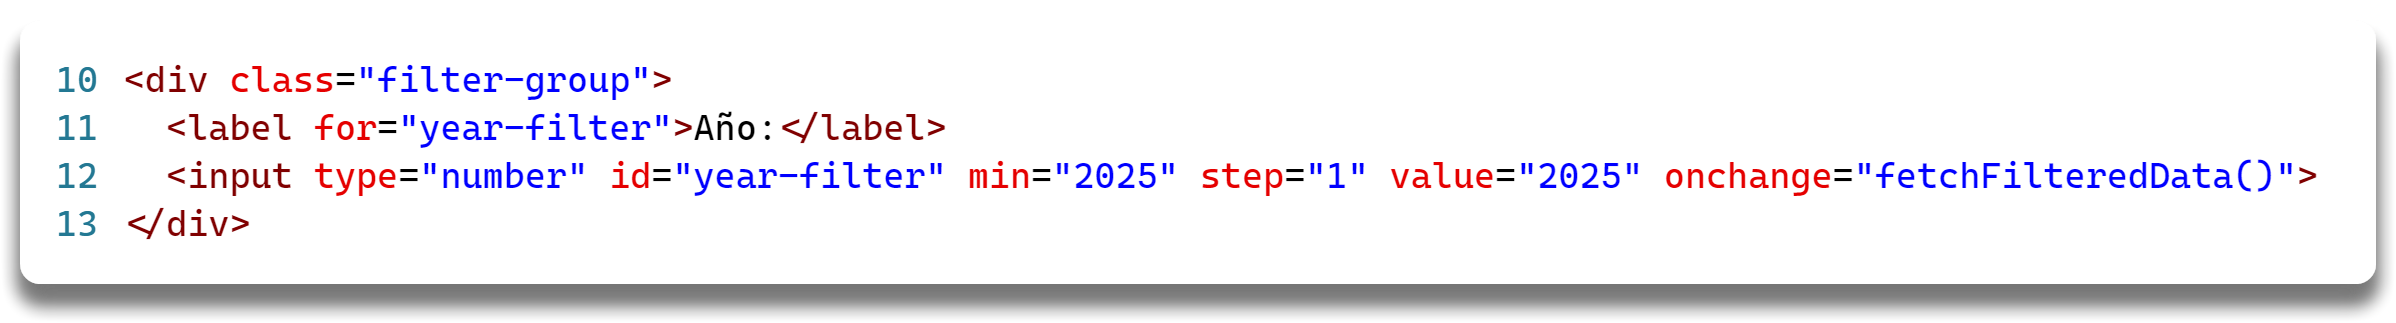
\includegraphics[width=\textwidth]{img/dashboardHTML2.png}
			            \caption{Archivo dashboard.html Parte II}
			            \label{fig:dashboardHTML2}
		            \end{figure}
		      \item Se pone un filtro para el mes:
		            \begin{figure}[H]
			            \centering
			            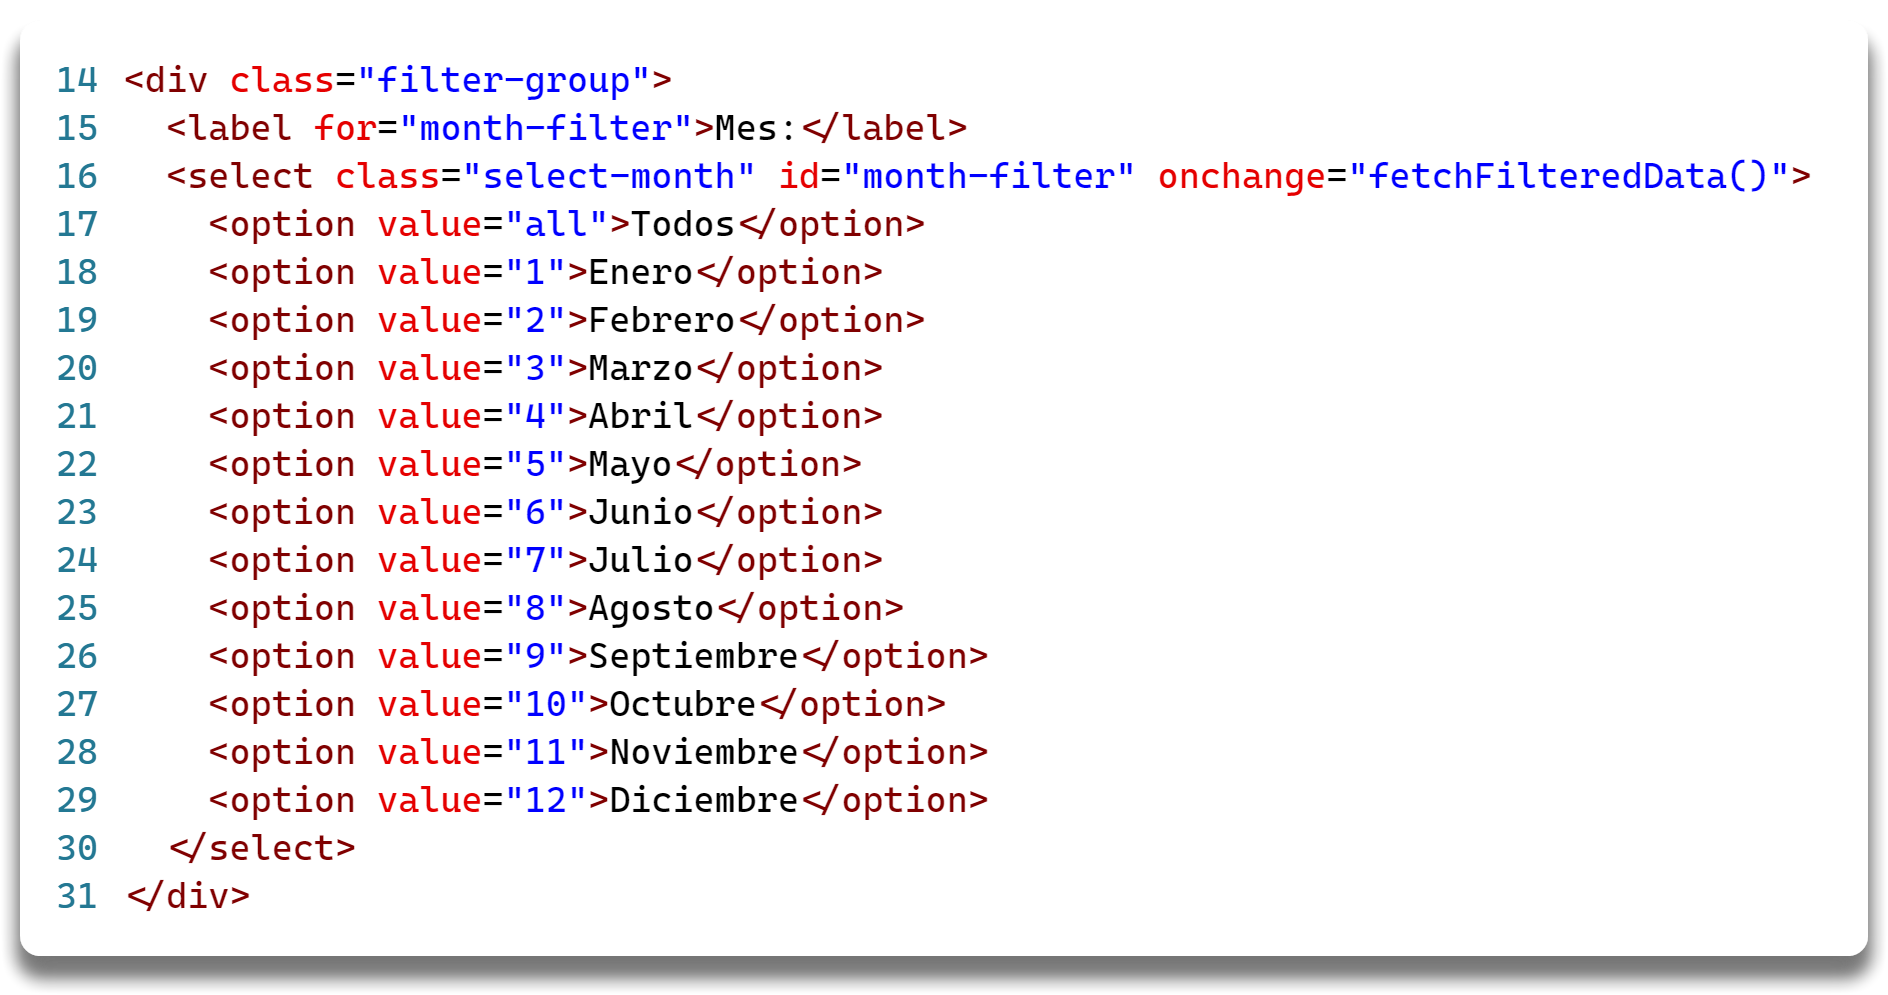
\includegraphics[width=\textwidth]{img/dashboardHTML3.png}
			            \caption{Archivo dashboard.html Parte III}
			            \label{fig:dashboardHTML3}
		            \end{figure}
		      \item Se pone un filtro para el día:
		            \begin{figure}[H]
			            \centering
			            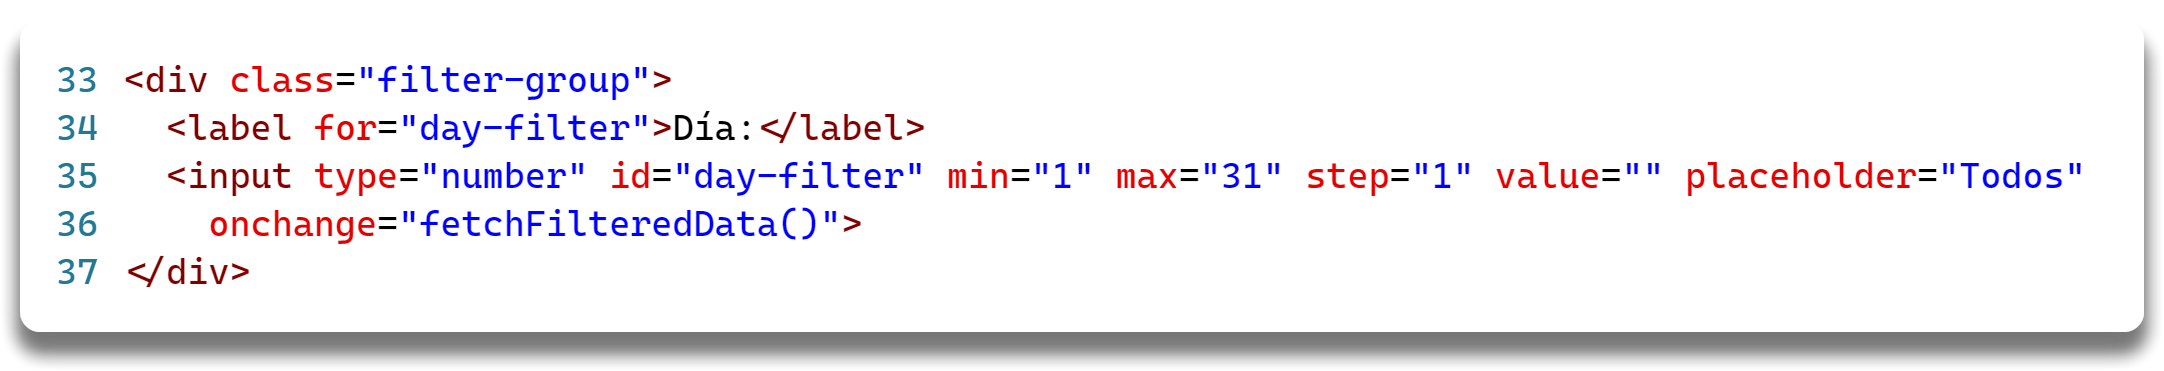
\includegraphics[width=\textwidth]{img/dashboardHTML4.png}
			            \caption{Archivo dashboard.html Parte IV}
			            \label{fig:dashboardHTML4}
		            \end{figure}
		            \newpage
		      \item Se pone un filtro para el motivo:
		            \begin{figure}[H]
			            \centering
			            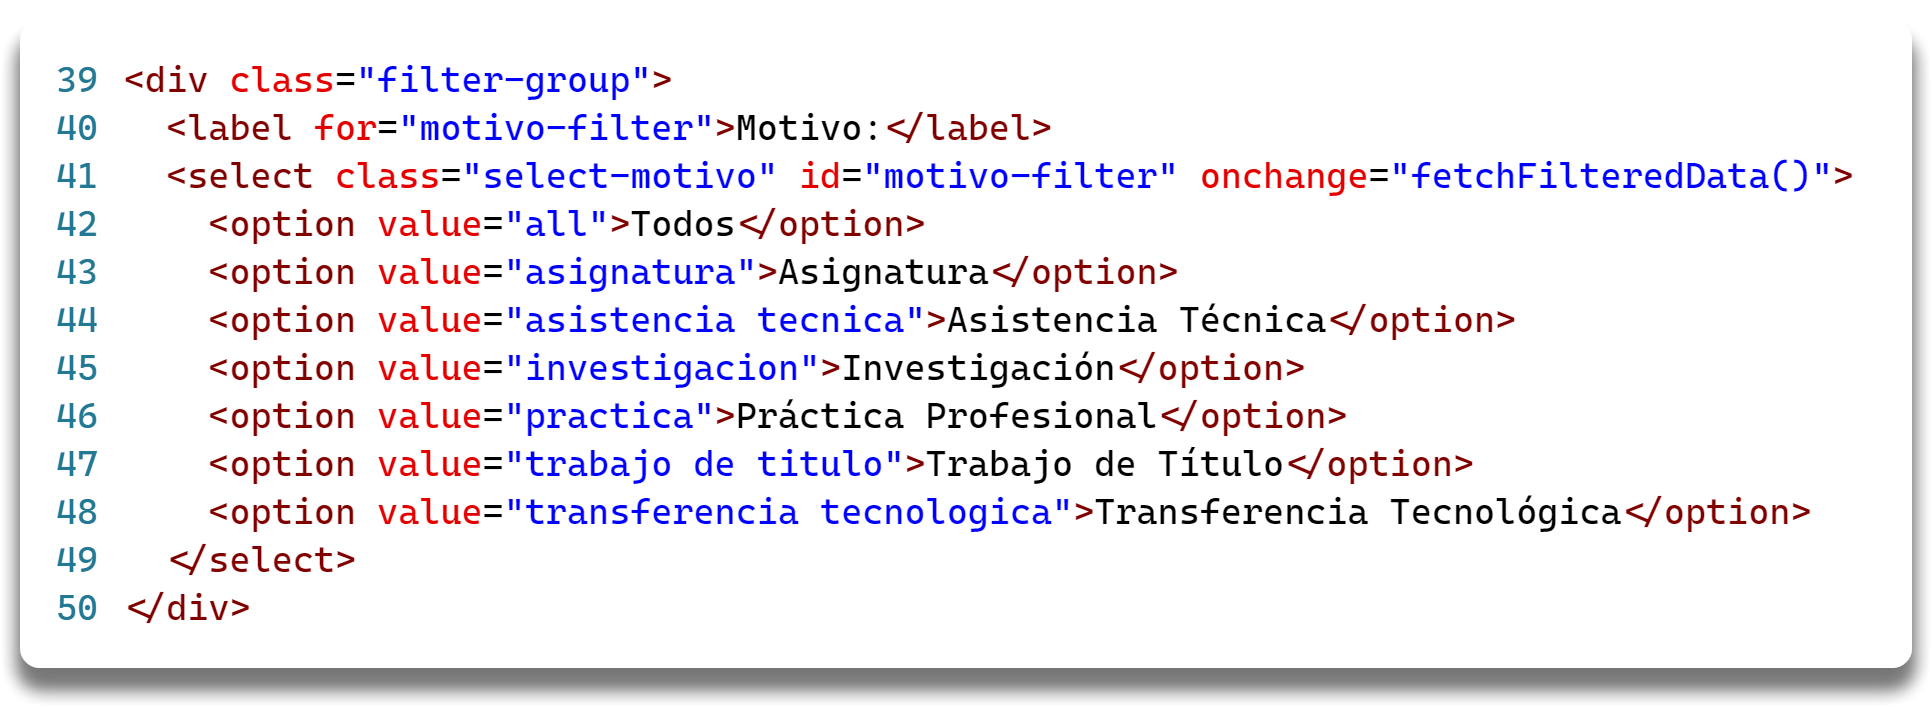
\includegraphics[width=\textwidth]{img/dashboardHTML5.png}
			            \caption{Archivo dashboard.html Parte V}
			            \label{fig:dashboardHTML5}
		            \end{figure}
		      \item Se pone un filtro para el rut:
		            \begin{figure}[H]
			            \centering
			            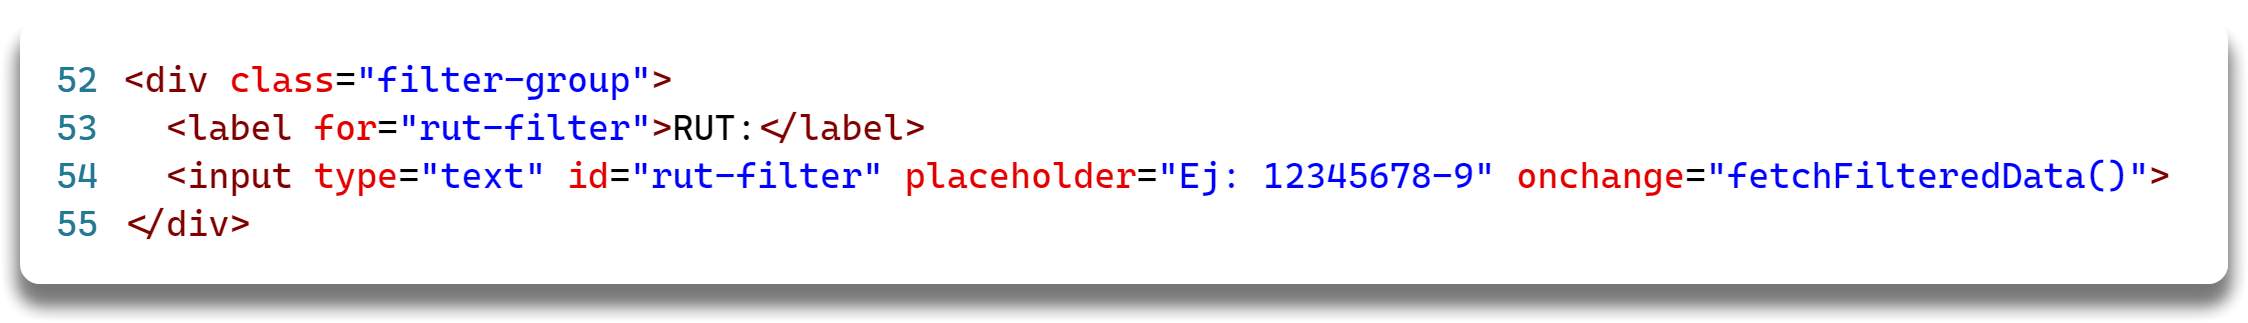
\includegraphics[width=\textwidth]{img/dashboardHTML6.png}
			            \caption{Archivo dashboard.html Parte VI}
			            \label{fig:dashboardHTML6}
		            \end{figure}
		      \item Se pone un boton para resetear los filtros a un valor por defecto:
		            \begin{figure}[H]
			            \centering
			            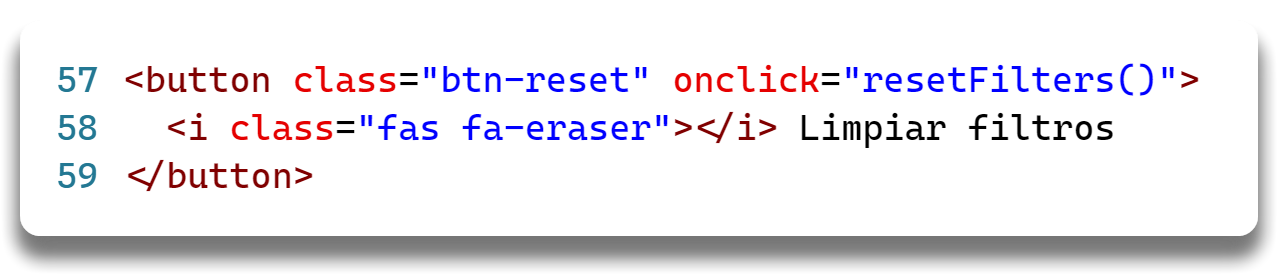
\includegraphics[width=\textwidth]{img/dashboardHTML7.png}
			            \caption{Archivo dashboard.html Parte VII}
			            \label{fig:dashboardHTML7}
		            \end{figure}
		      \item Se pone un boton para mostrar/esconder el SIDEBAR:
		            \begin{figure}[H]
			            \centering
			            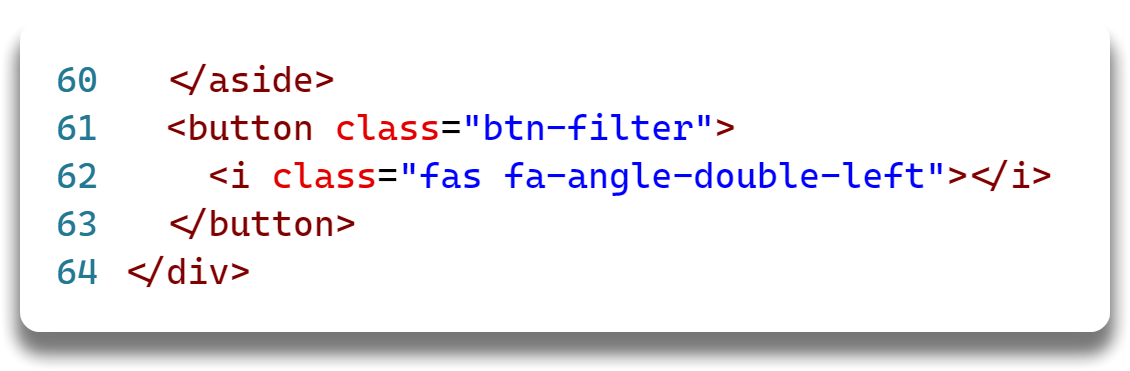
\includegraphics[width=0.6\textwidth]{img/dashboardHTML8.png}
			            \caption{Archivo dashboard.html Parte VIII}
			            \label{fig:dashboardHTML8}
		            \end{figure}
		      \item Se pone una secci\'on para mostrar la estadistica del total de horas y total de usuarios que han utilizado el laboratorio:
		            \begin{figure}[H]
			            \centering
			            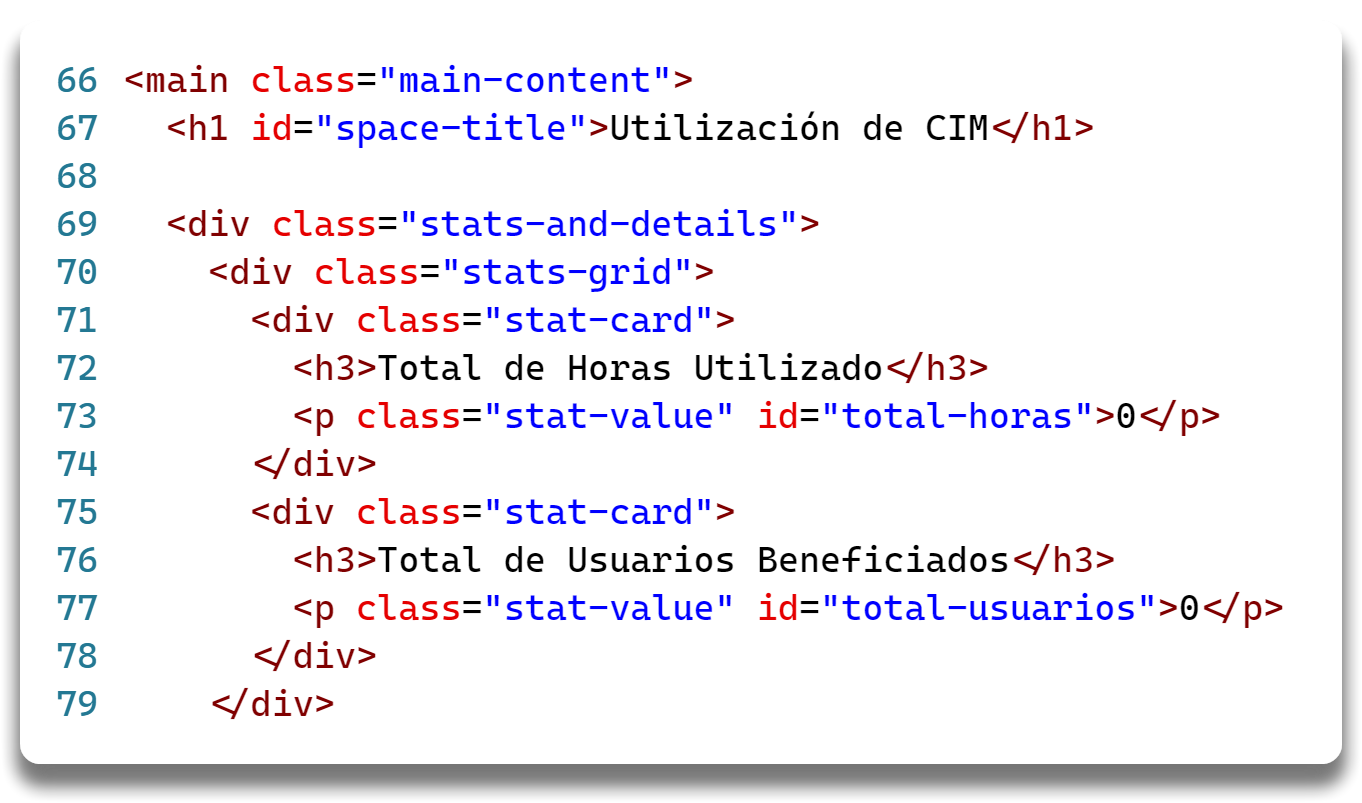
\includegraphics[width=0.8\textwidth]{img/dashboardHTML9.png}
			            \caption{Archivo dashboard.html Parte IX}
			            \label{fig:dashboardHTML9}
		            \end{figure}
		      \item Se pone una secci\'on para mostrar la tabla de registros desde el m\'as reciente al m\'as antiguo:
		            \begin{figure}[H]
			            \centering
			            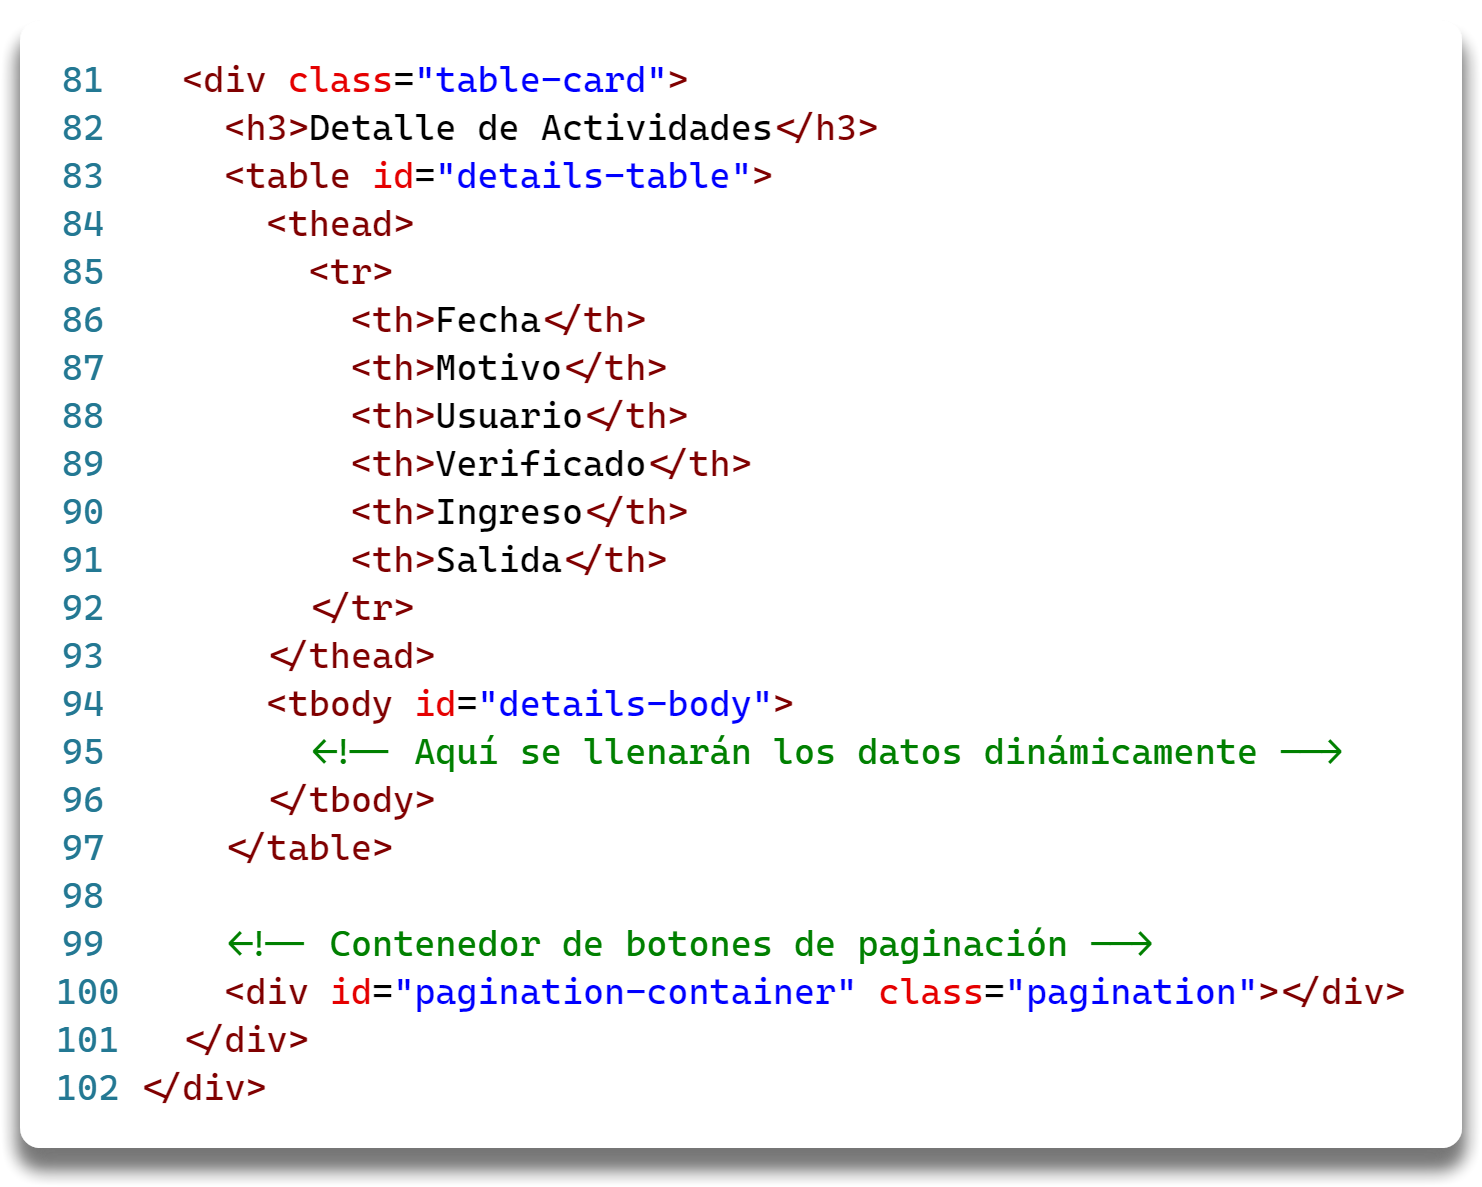
\includegraphics[width=0.8\textwidth]{img/dashboardHTML10.png}
			            \caption{Archivo dashboard.html Parte X}
			            \label{fig:dashboardHTML10}
		            \end{figure}
		            \newpage
		      \item Se pone una secci\'on para mostrar algunas gr\'aficas:
		            \begin{figure}[H]
			            \centering
			            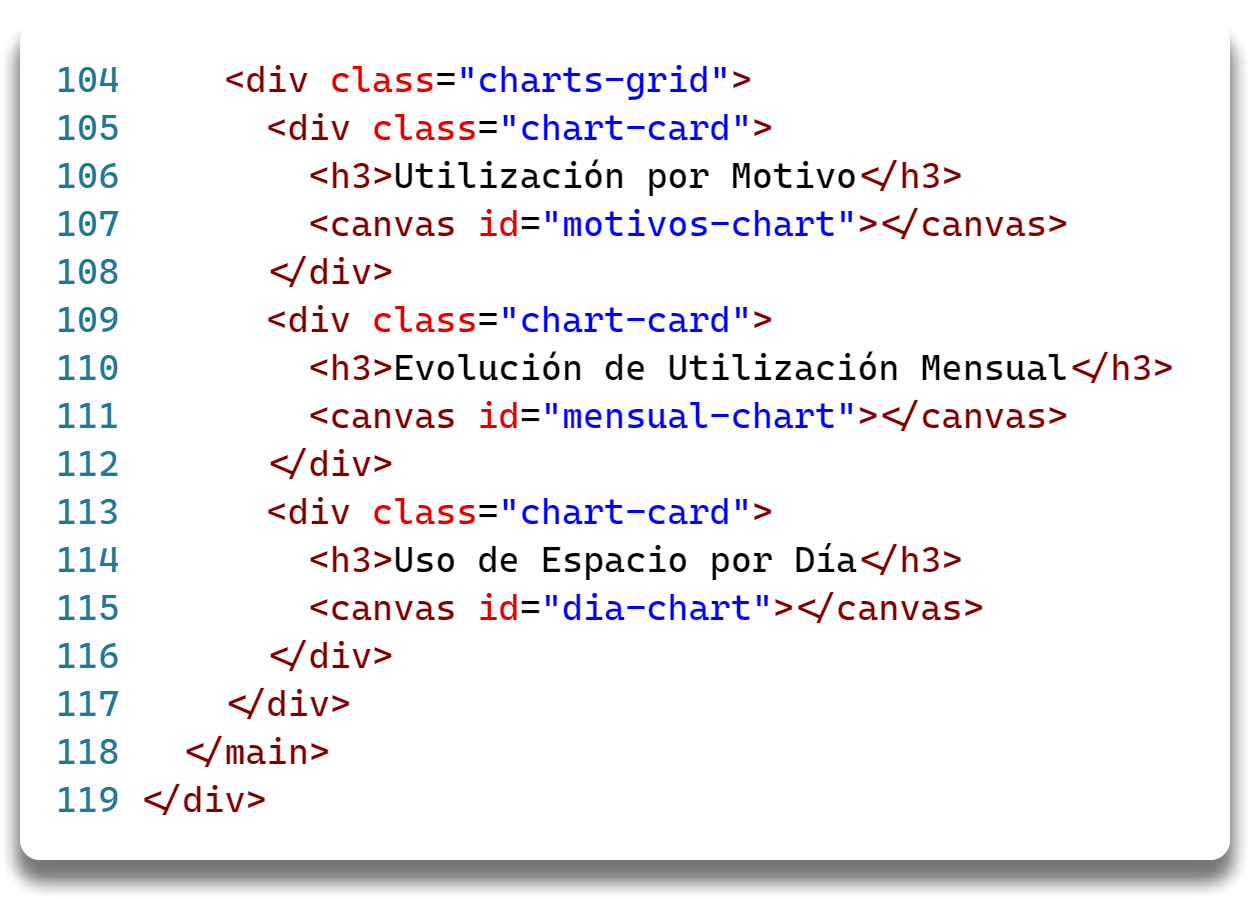
\includegraphics[width=0.8\textwidth]{img/dashboardHTML11.png}
			            \caption{Archivo dashboard.html Parte XI}
			            \label{fig:dashboardHTML11}
		            \end{figure}
		      \item Se agregan los scripts y una función para mostrar el correcto registro de un usuario o administrador:
		            \begin{figure}[H]
			            \centering
			            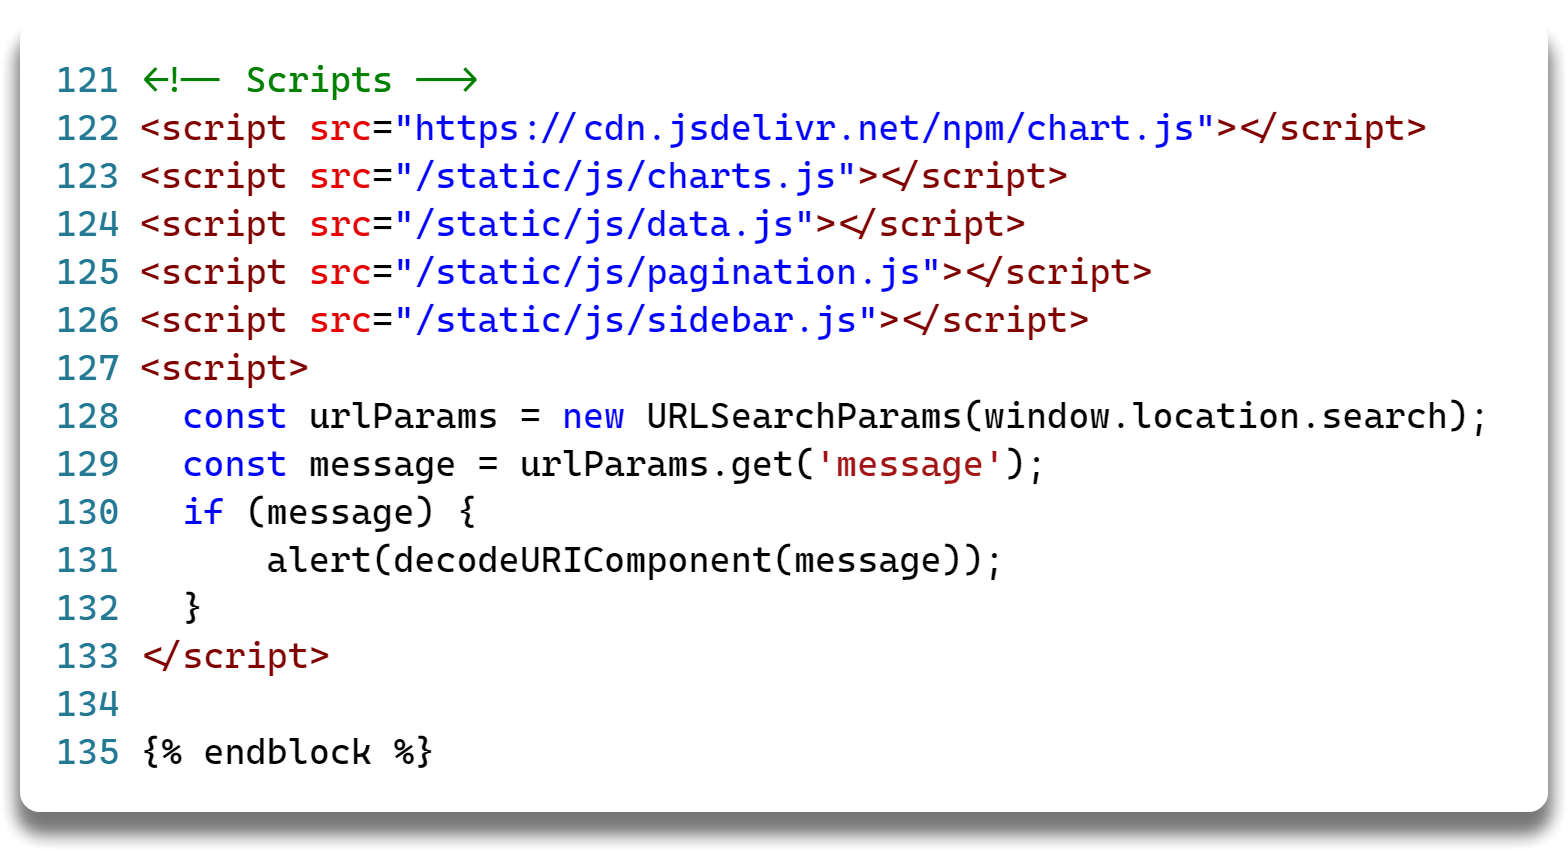
\includegraphics[width=\textwidth]{img/dashboardHTML12.png}
			            \caption{Archivo dashboard.html Parte XII}
			            \label{fig:dashboardHTML12}
		            \end{figure}
	      \end{enumerate}
	      \newpage
	\item \textbf{charts.js}:
	      \begin{enumerate}
		      \item Etiquetas para los meses:
		            \begin{figure}[H]
			            \centering
			            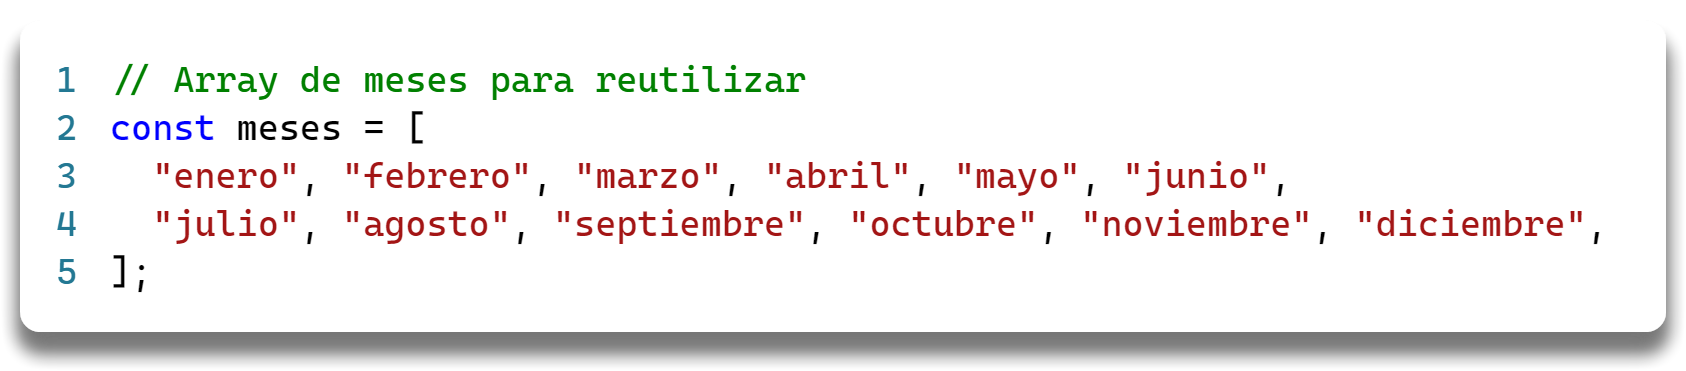
\includegraphics[width=\textwidth]{img/chartsJS1.png}
			            \caption{Archivo charts.js Parte I}
			            \label{fig:chartsJS1}
		            \end{figure}
		      \item Configuración gr\'afica de barra por motivo:
		            \begin{figure}[H]
			            \centering
			            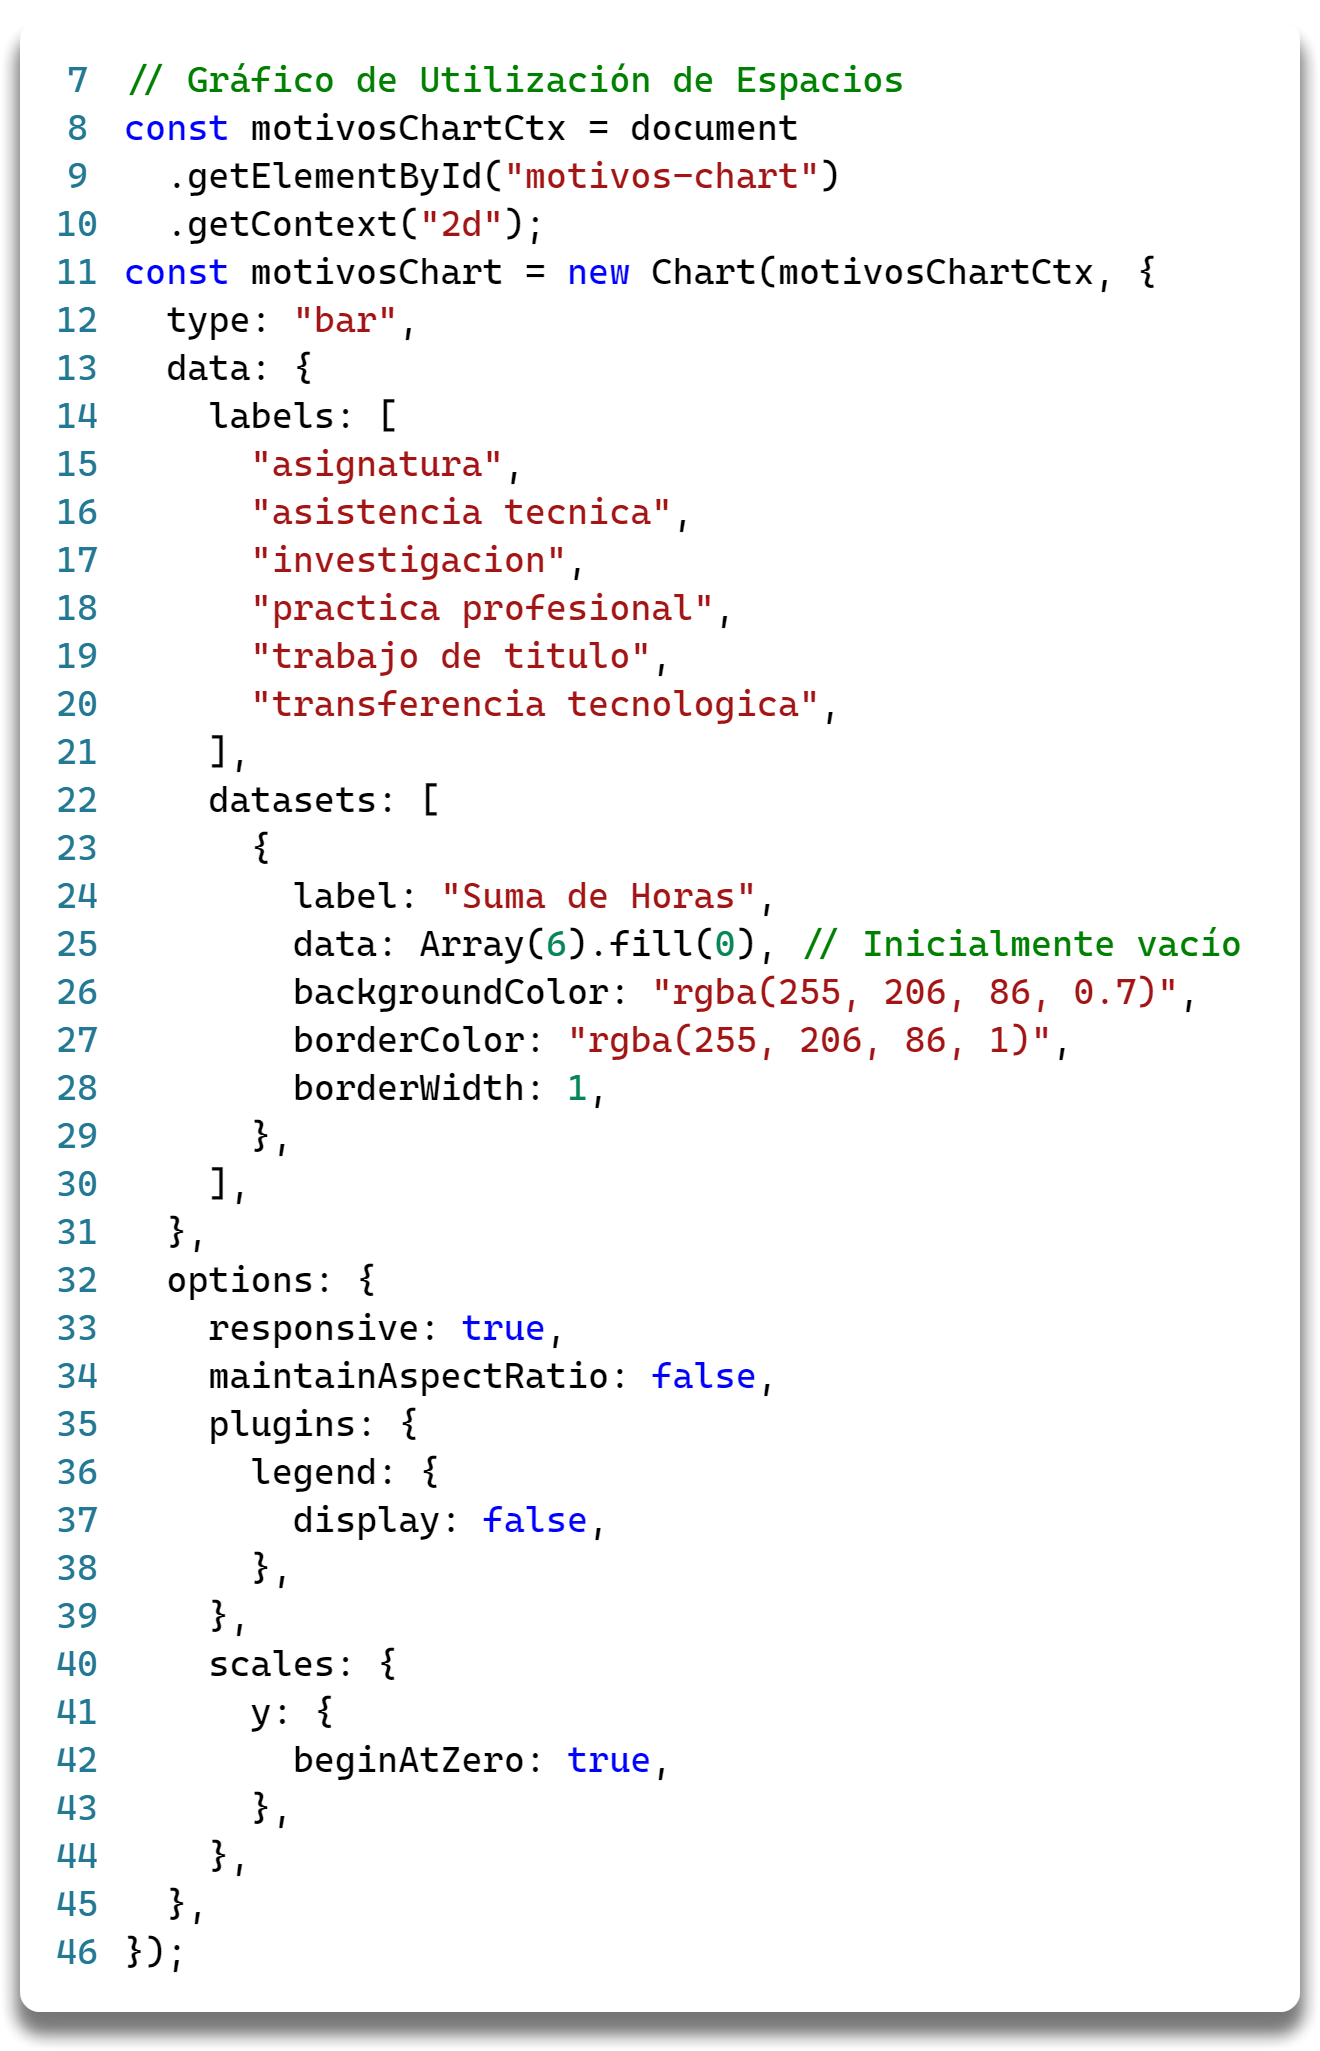
\includegraphics[width=0.6\textwidth]{img/chartsJS2.png}
			            \caption{Archivo charts.js Parte II}
			            \label{fig:chartsJS2}
		            \end{figure}
		      \item Configuración gr\'afica de puntos evoluci\'on de utilizaci\'on mensual:
		            \begin{figure}[H]
			            \centering
			            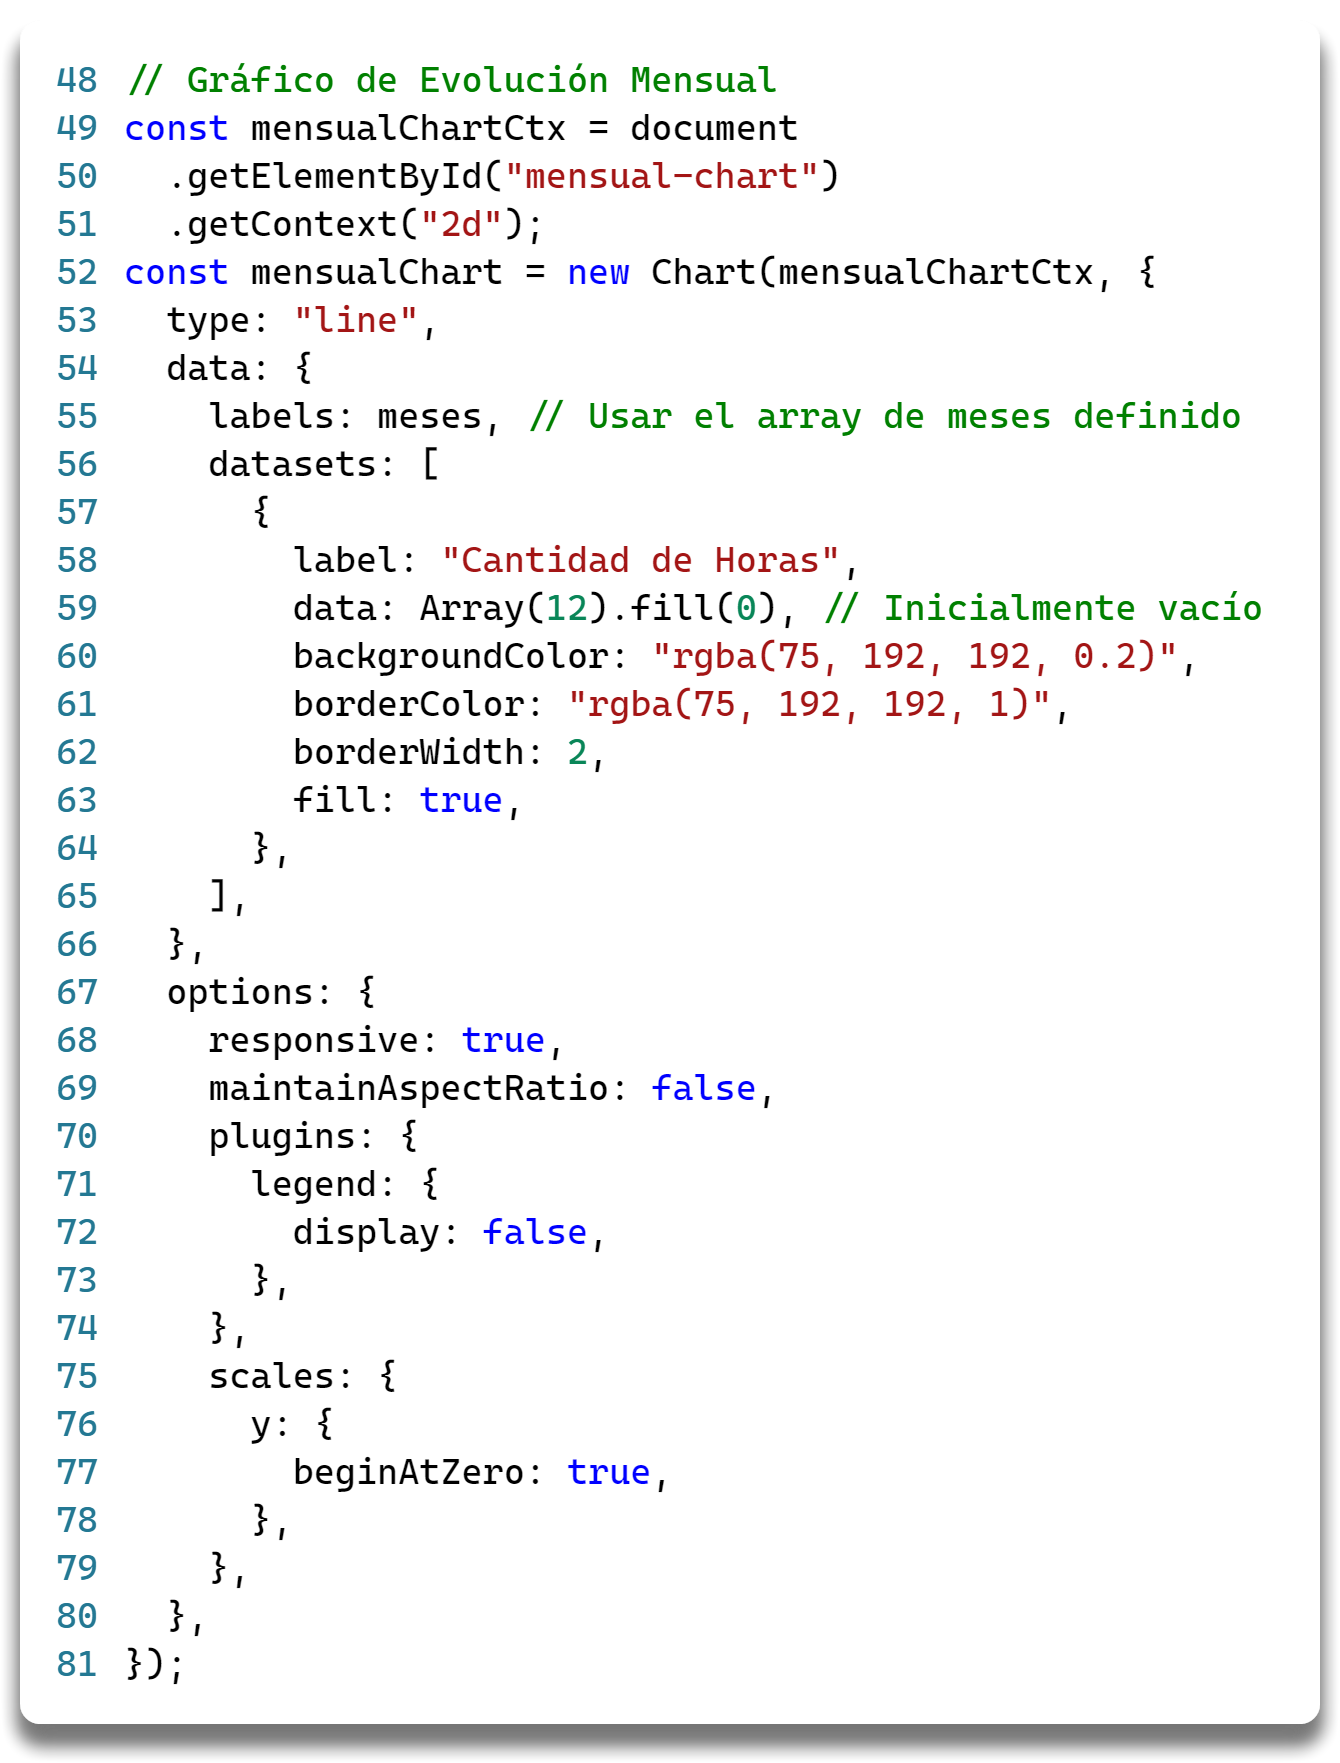
\includegraphics[width=\textwidth]{img/chartsJS3.png}
			            \caption{Archivo charts.js Parte III}
			            \label{fig:chartsJS3}
		            \end{figure}
		            \newpage
		      \item Configuración gr\'afica de barra por uso de d\'ia:
		            \begin{figure}[H]
			            \centering
			            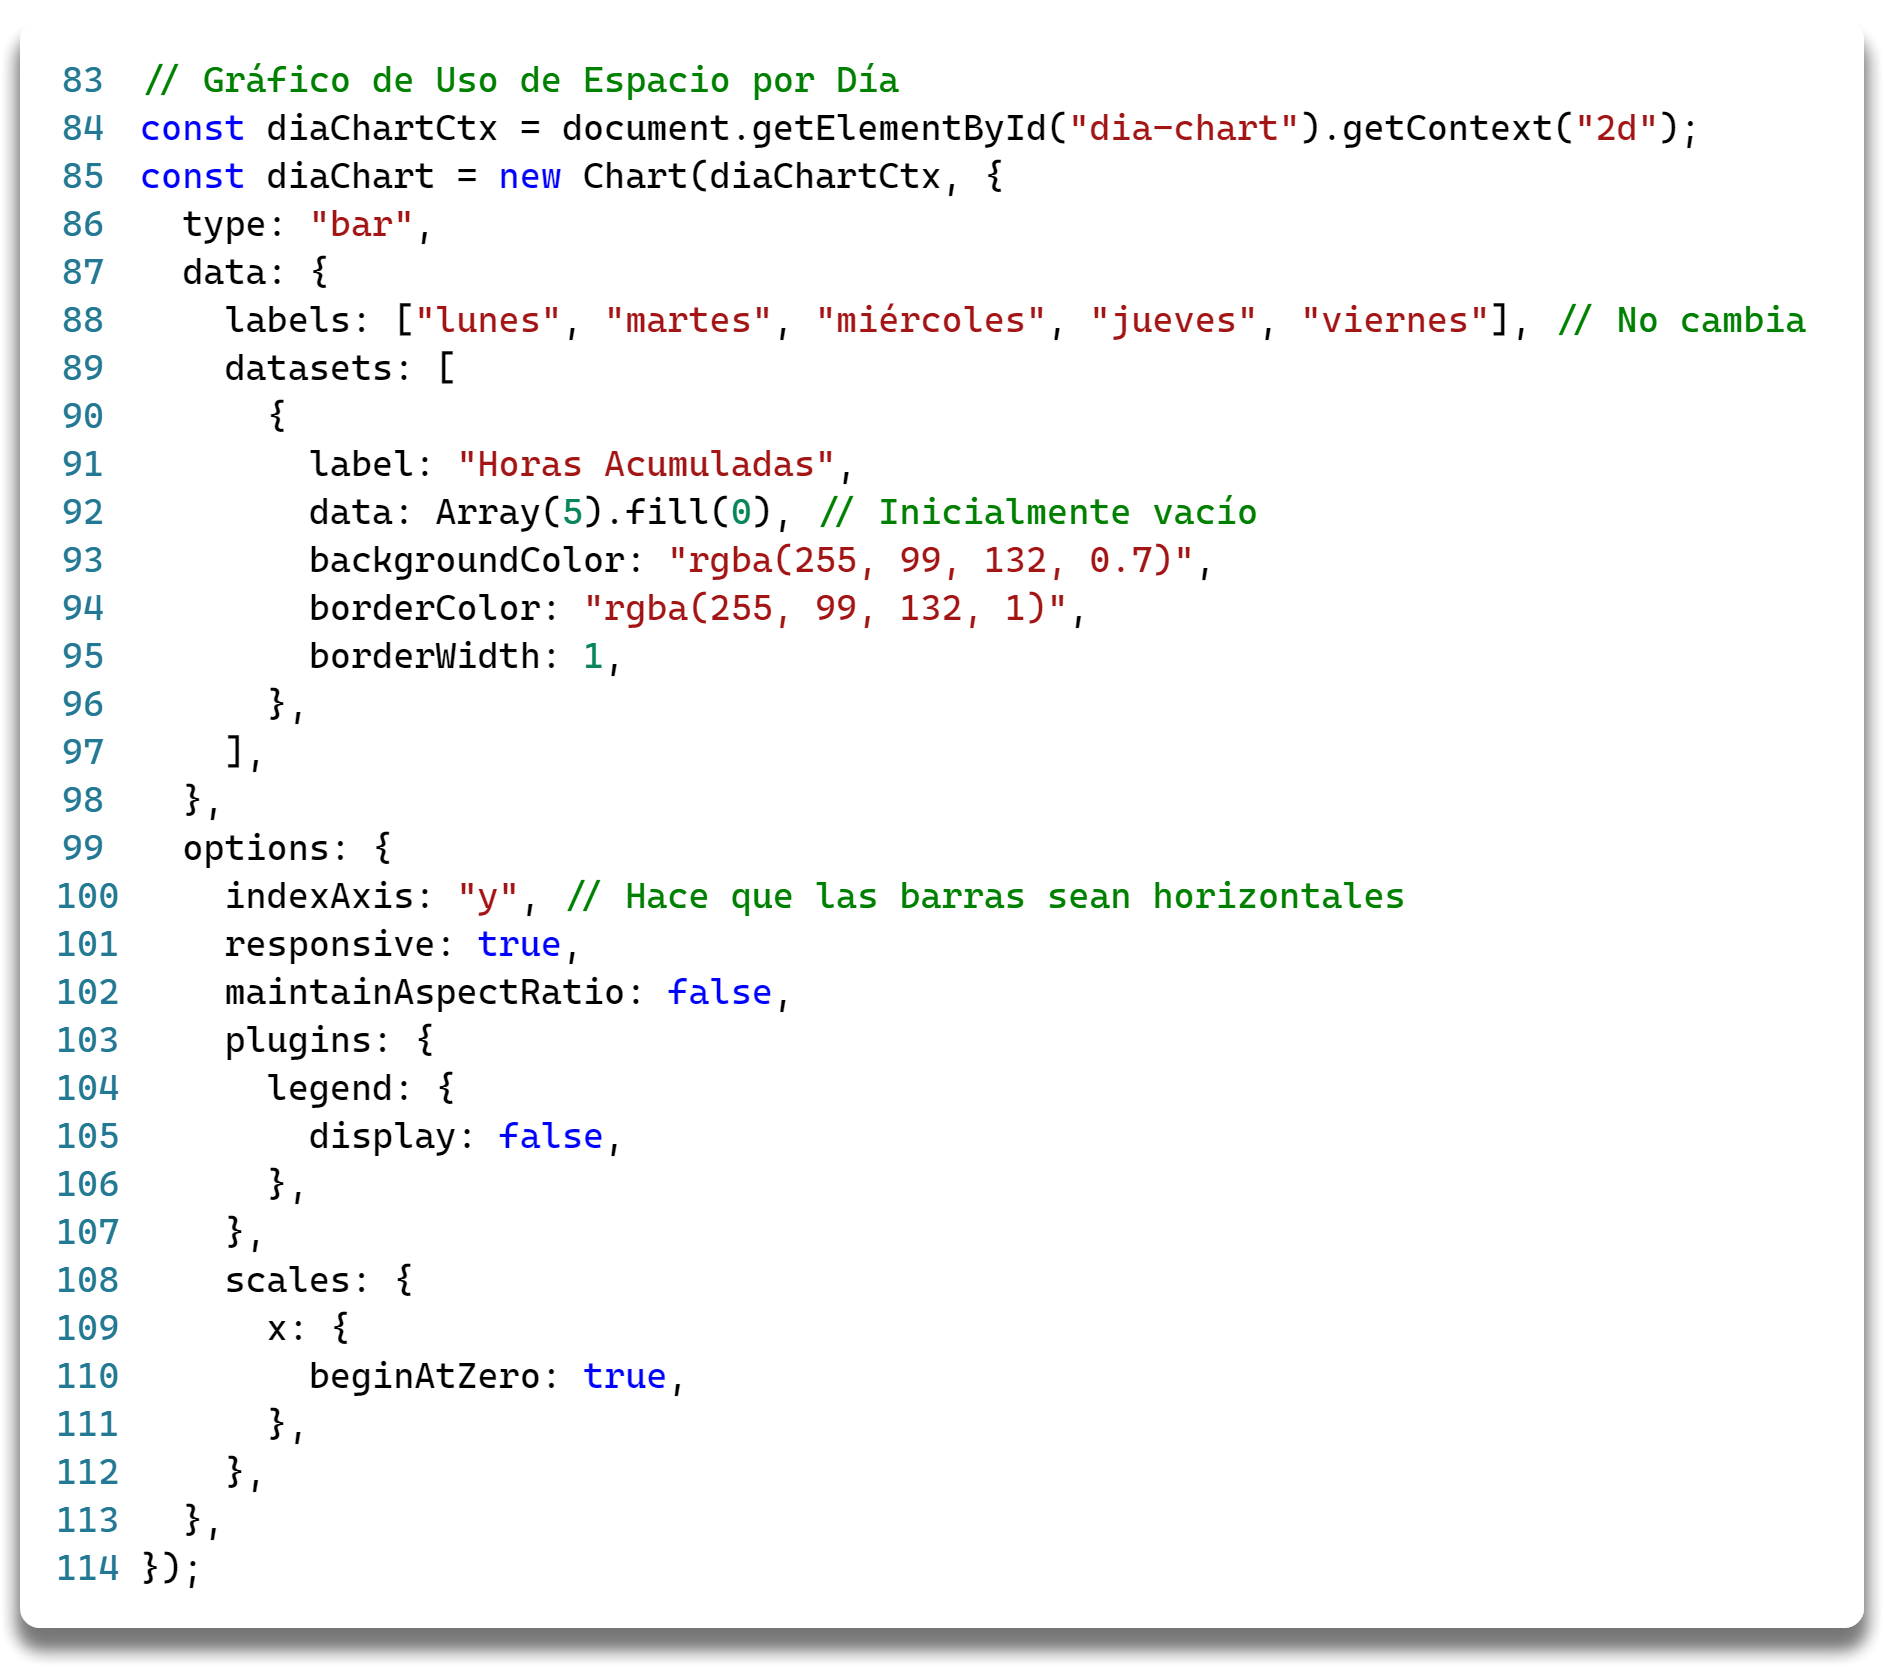
\includegraphics[width=\textwidth]{img/chartsJS4.png}
			            \caption{Archivo charts.js Parte IV}
			            \label{fig:chartsJS4}
		            \end{figure}
	      \end{enumerate}
\newpage
		  \item \textbf{data.js}:
		  \begin{enumerate}
			\item Función que se encarga de obtener los valores de los filtros, crear la petici\'on a la API y actualizar los datos:
			\begin{figure}[H]
				\centering
				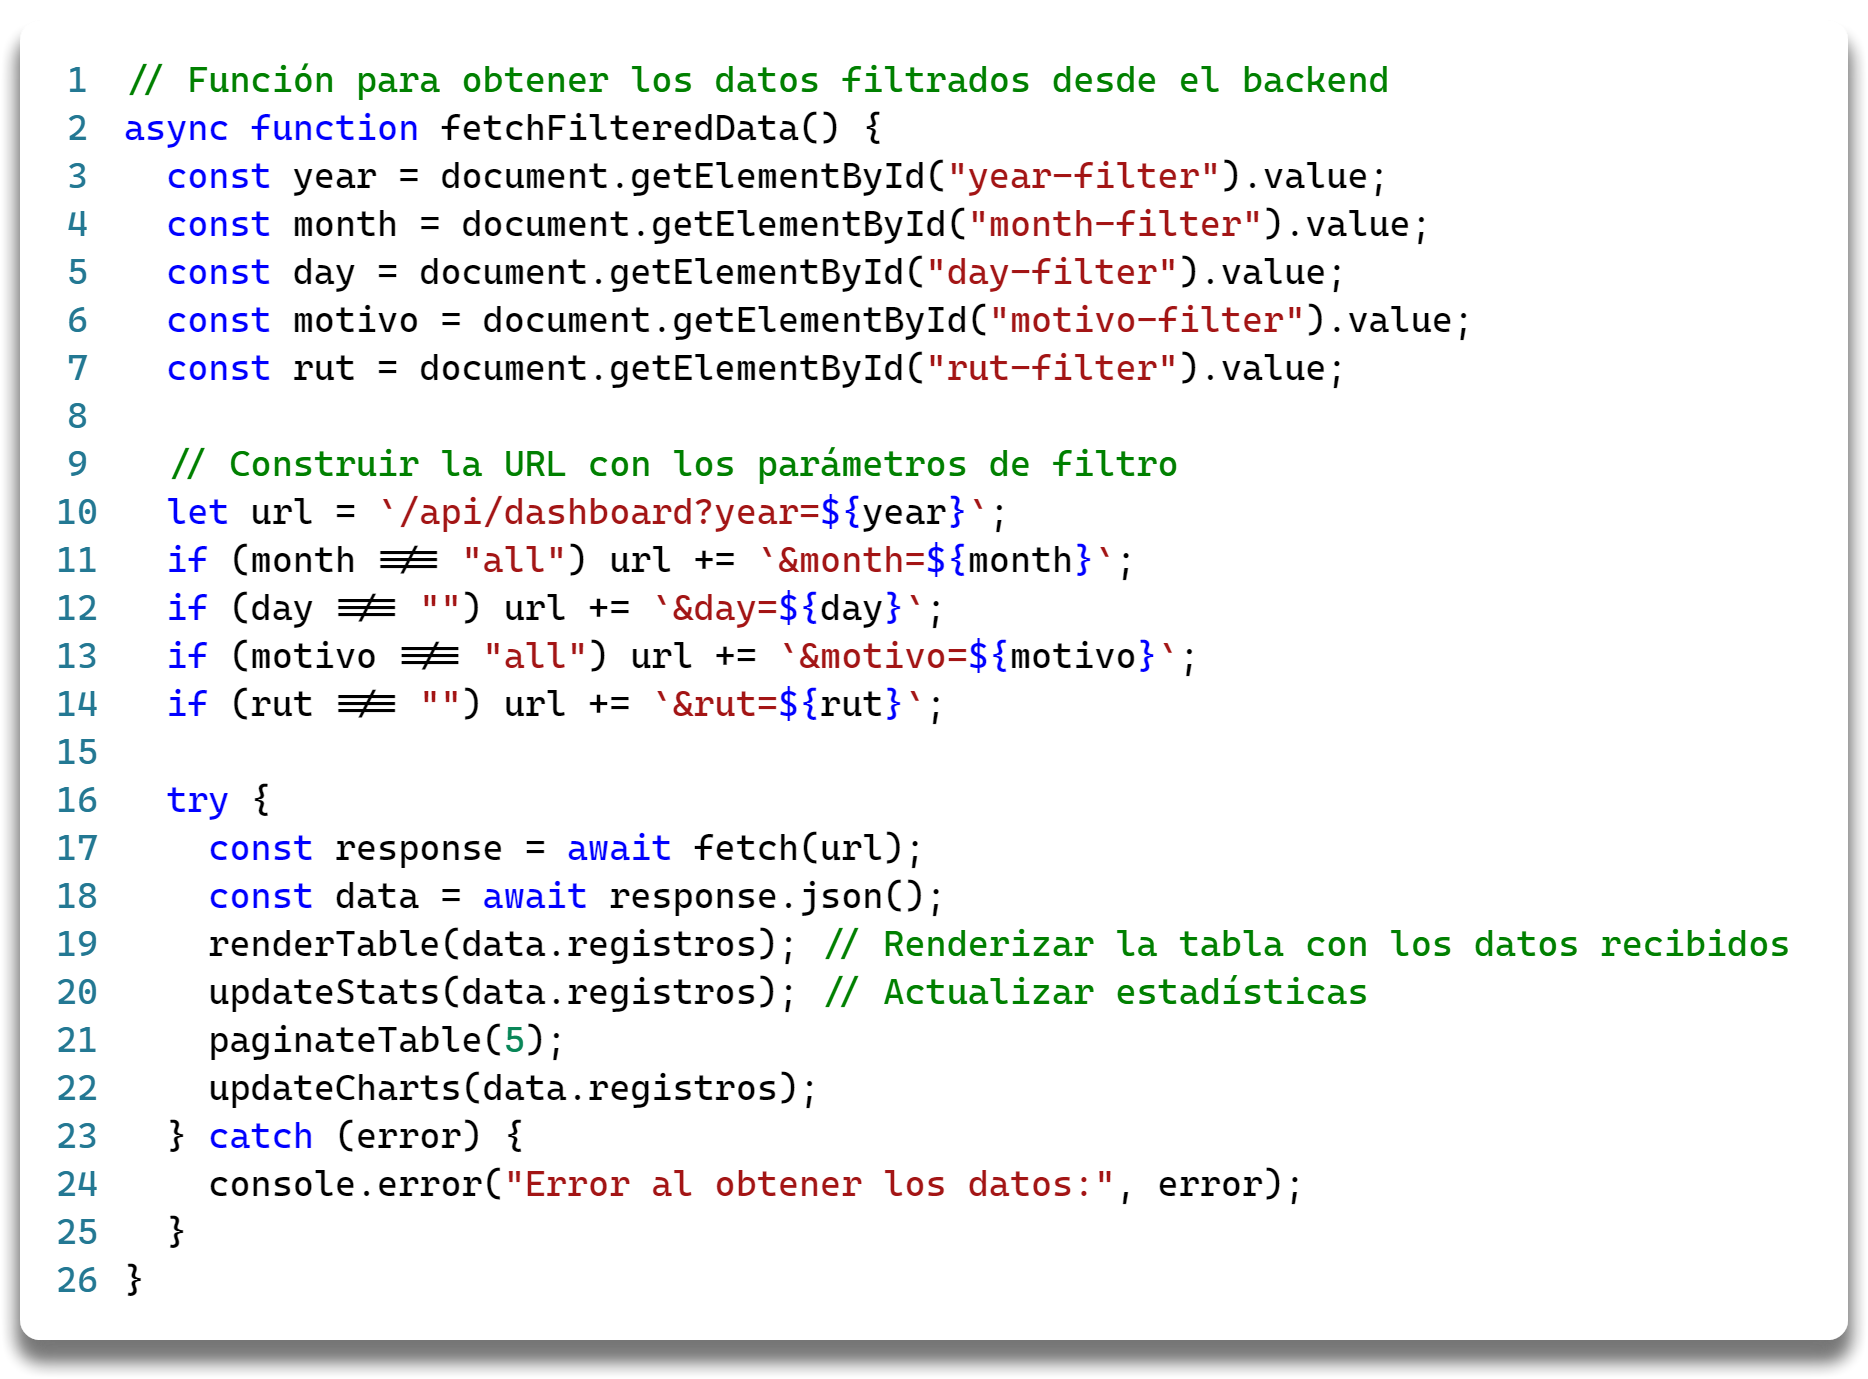
\includegraphics[width=\textwidth]{img/dataJS1.png}
				\caption{Archivo data.js Parte I}
				\label{fig:dataJS1}
			\end{figure}
			\newpage
			\item Función que se encarga de renderizar y formatear los datos de la tabla:
			\begin{figure}[H]
				\centering
				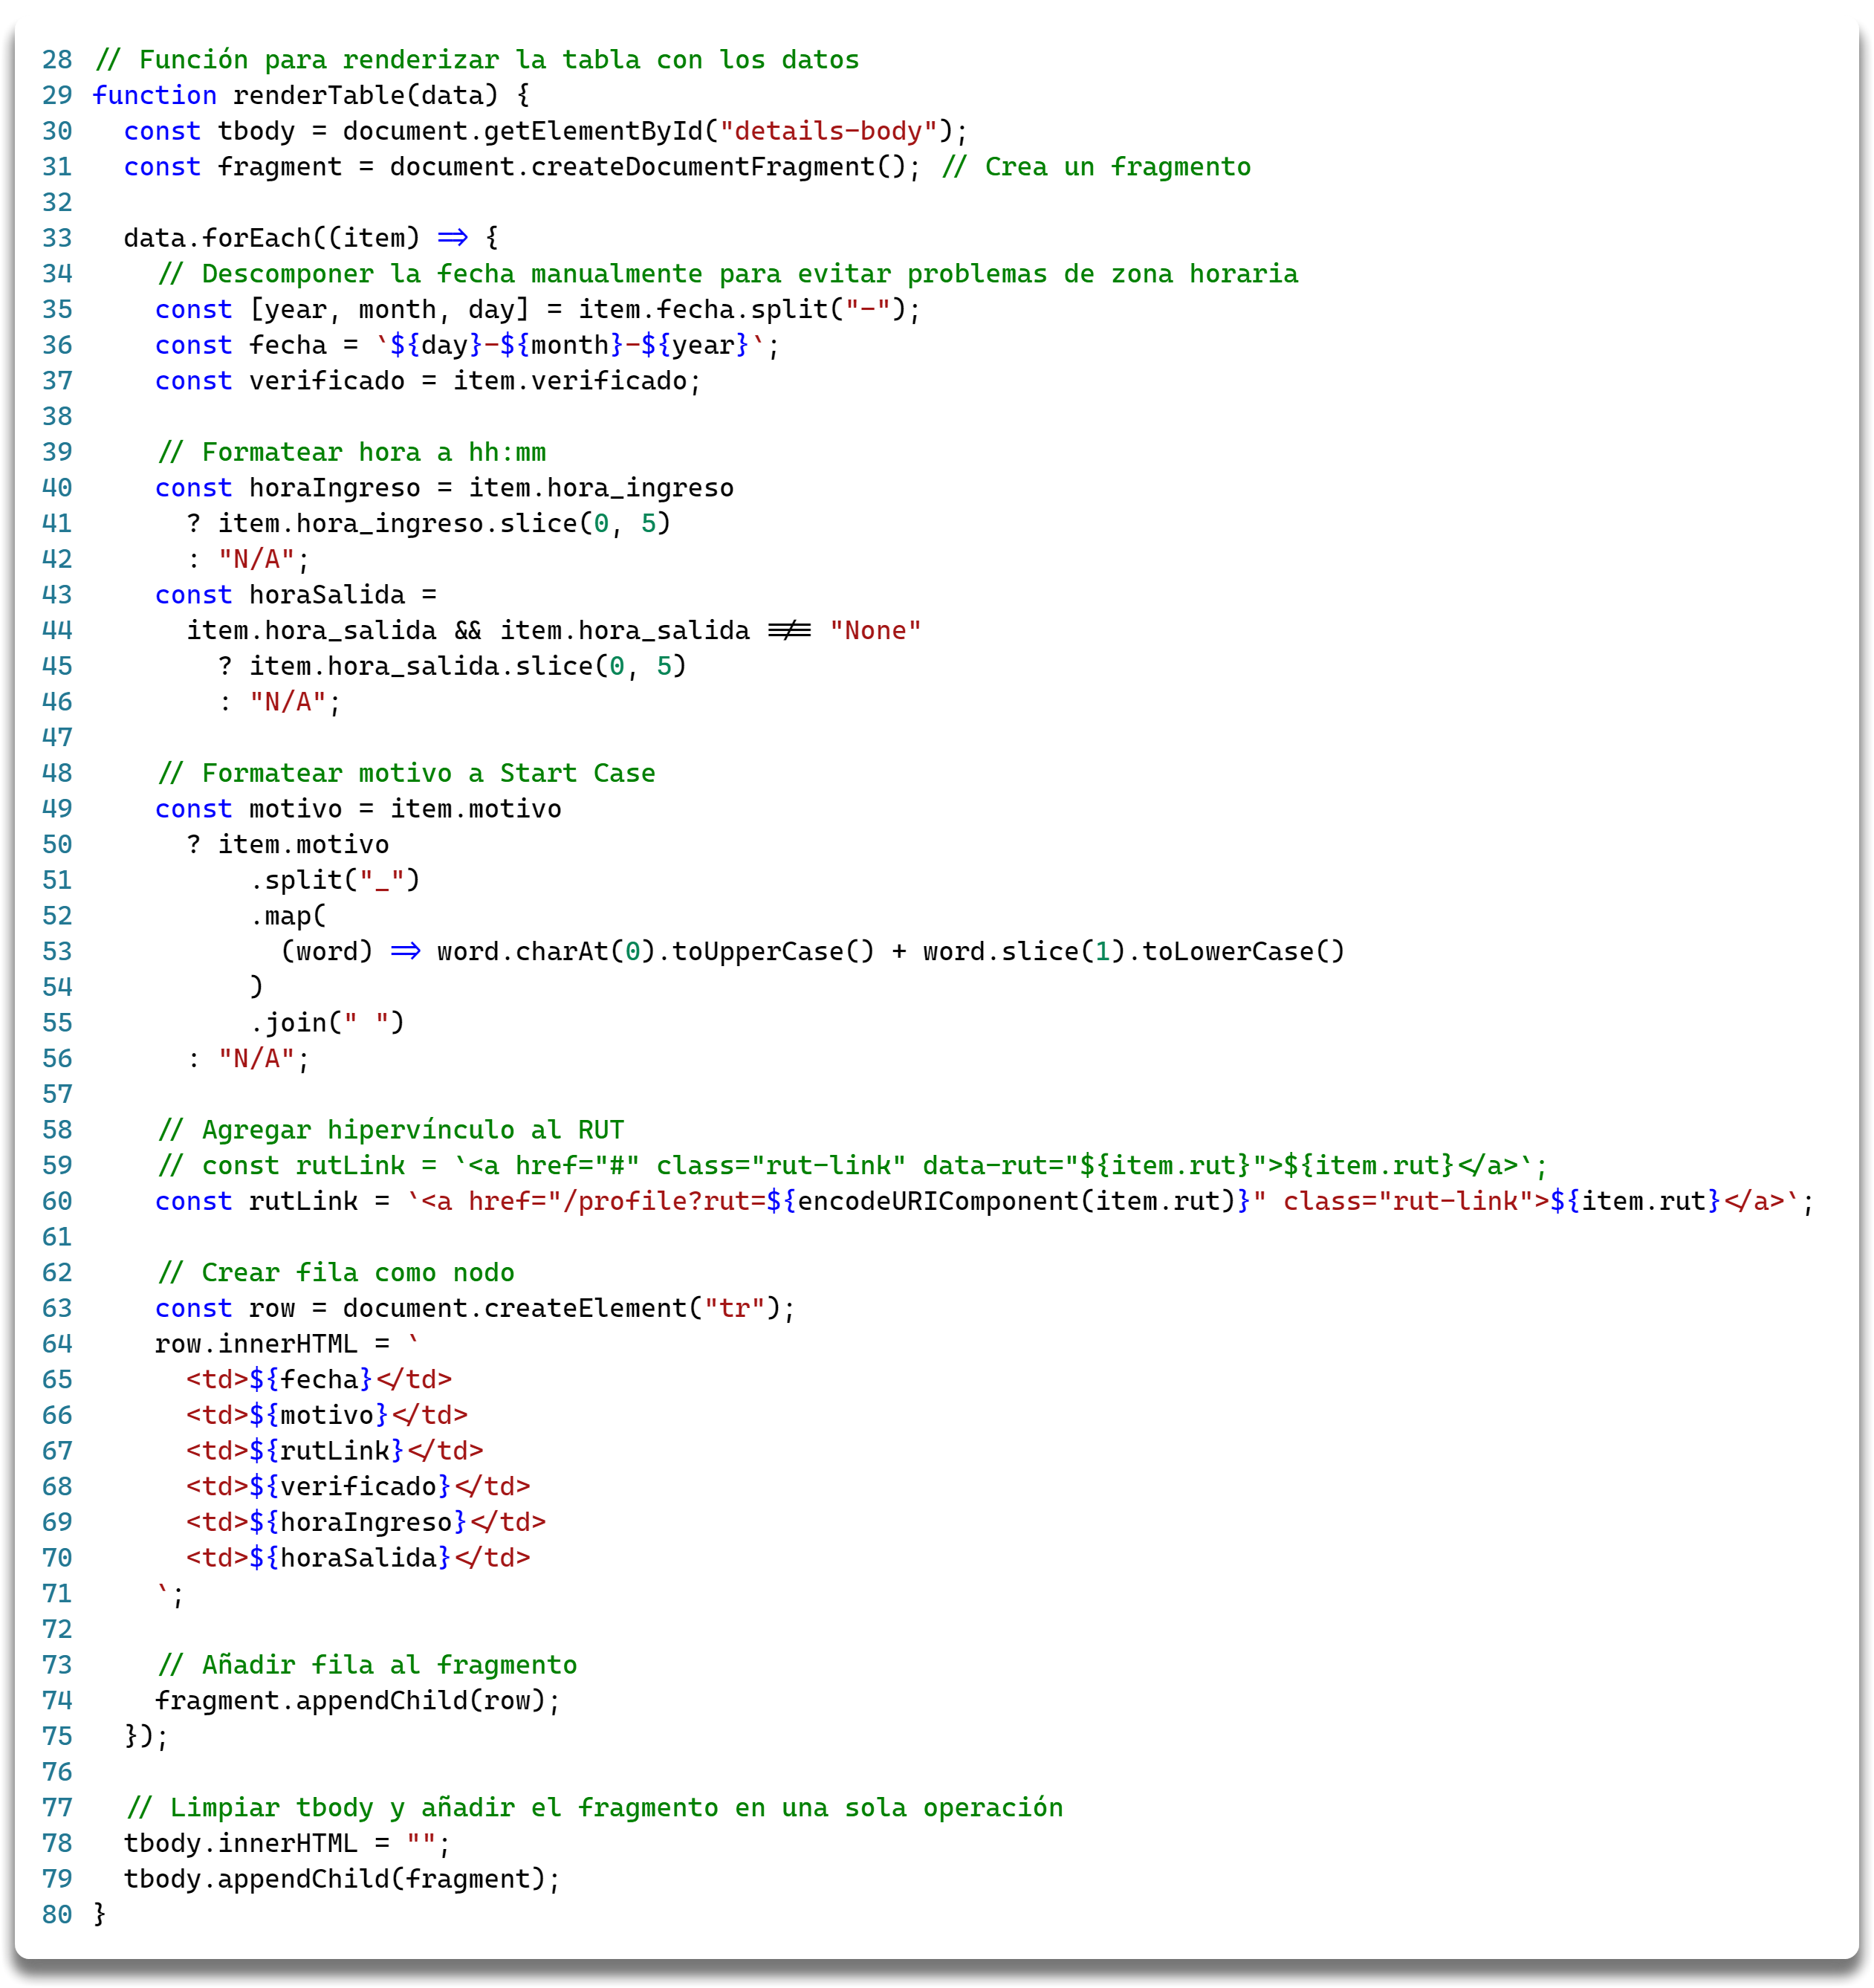
\includegraphics[width=\textwidth]{img/dataJS2.png}
				\caption{Archivo data.js Parte II}
				\label{fig:dataJS2}
			\end{figure}
			\newpage
			\item Funci\'on que se encarga de calcular las estadisticas del total de usuarios y la cantidad de horas:
			\begin{figure}[H]
				\centering
				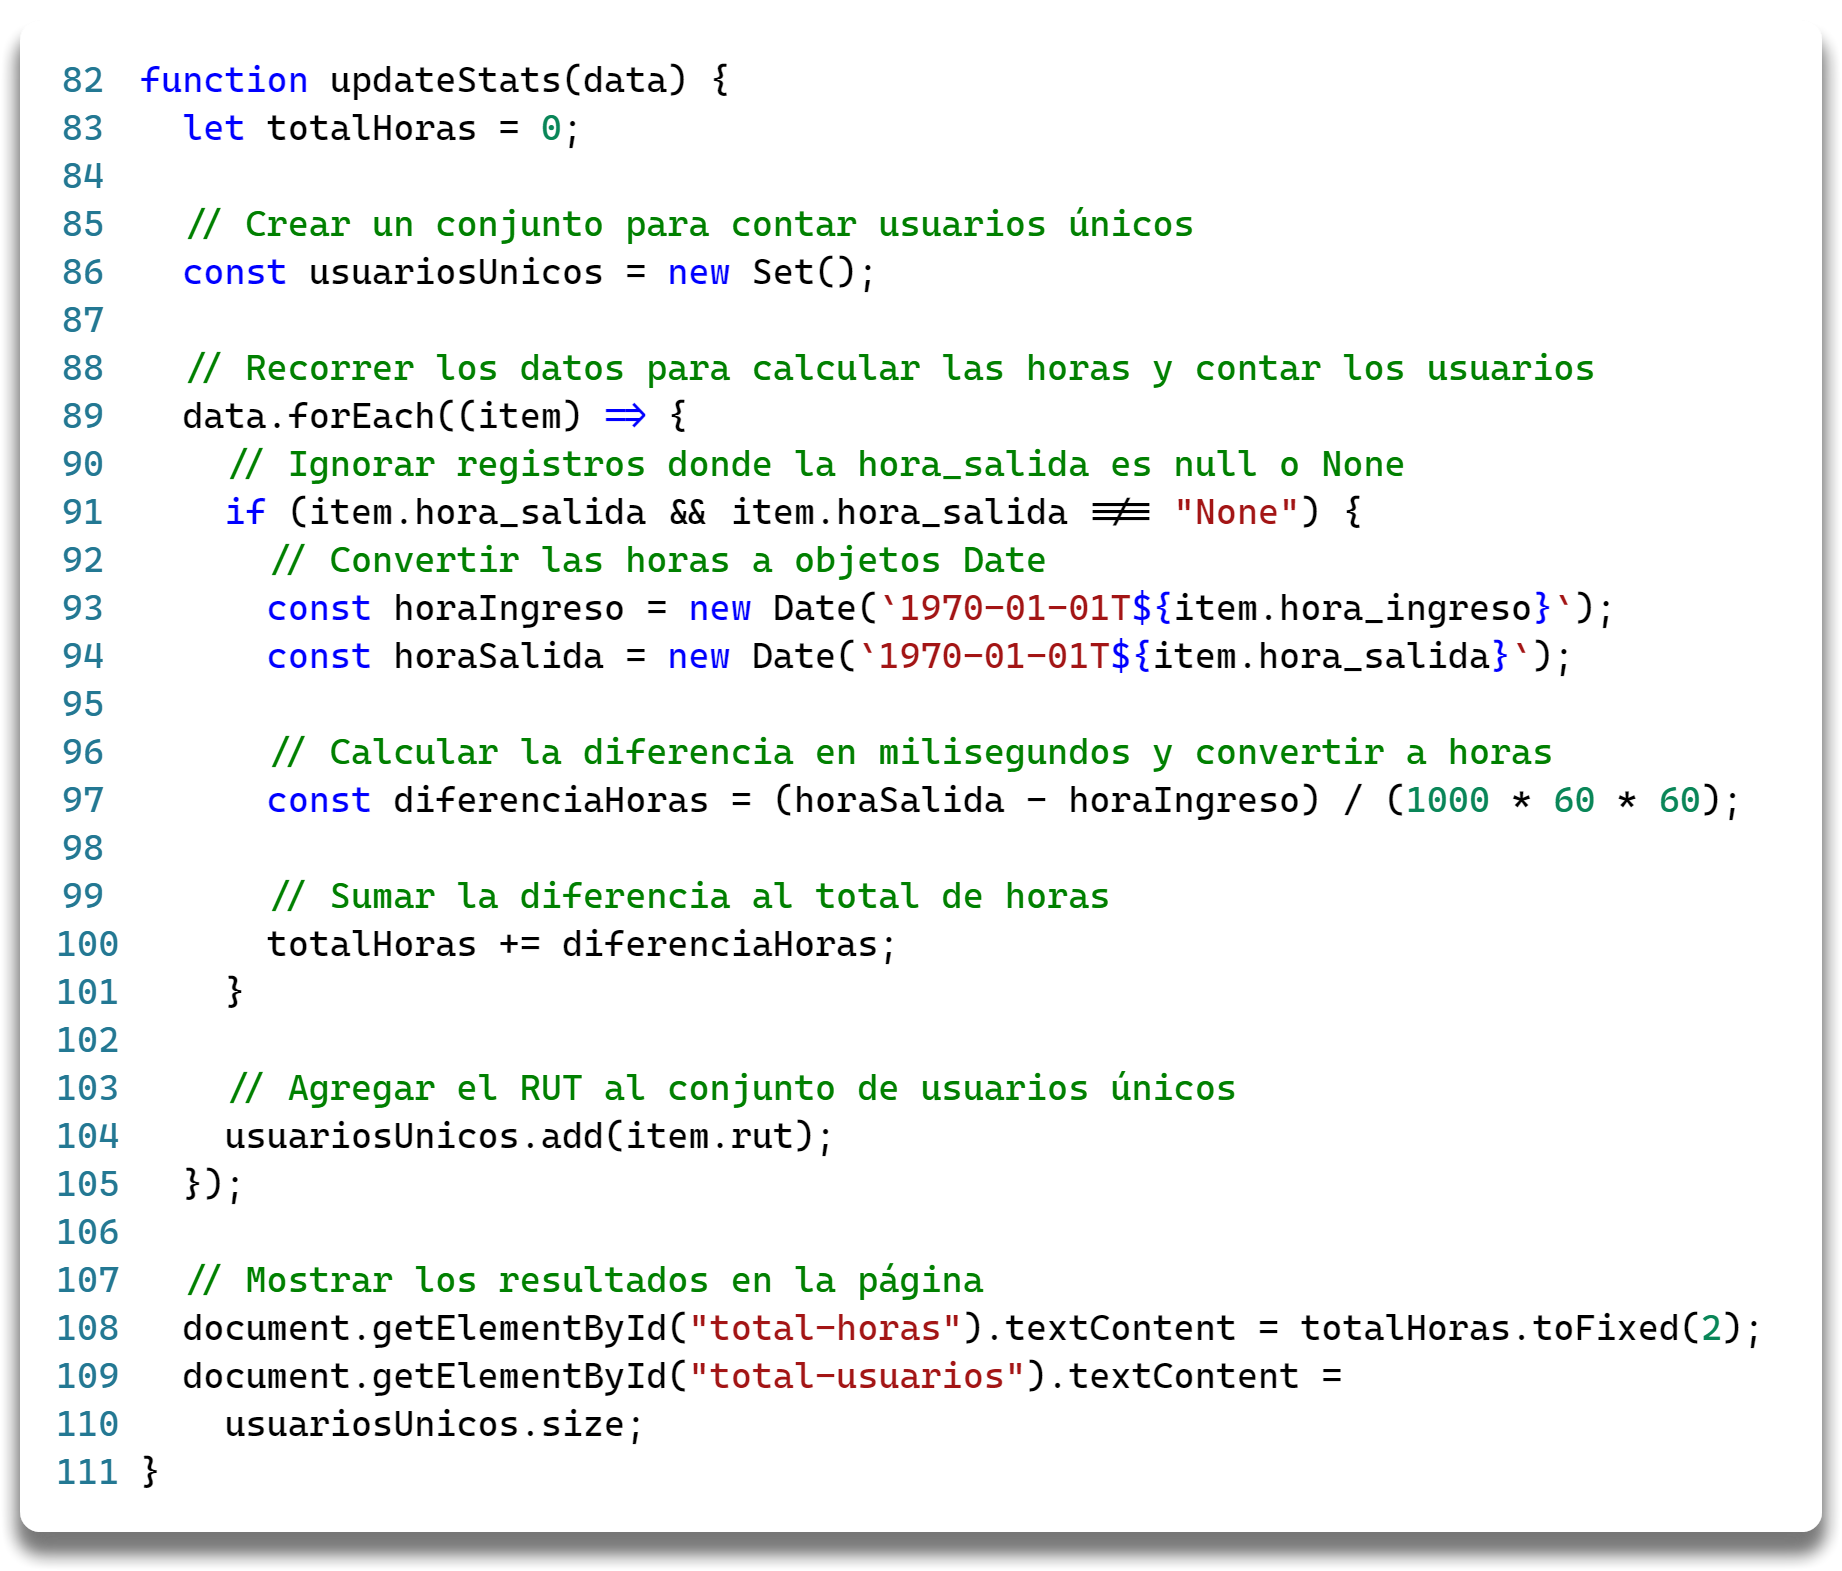
\includegraphics[width=\textwidth]{img/dataJS3.png}
				\caption{Archivo data.js Parte III}
				\label{fig:dataJS3}
			\end{figure}
			\newpage
			\item Función que se encarga de actualizar la información de las gr\'aficas, definici\'on de etiquetas par temas de acentos:
			\begin{figure}[H]
				\centering
				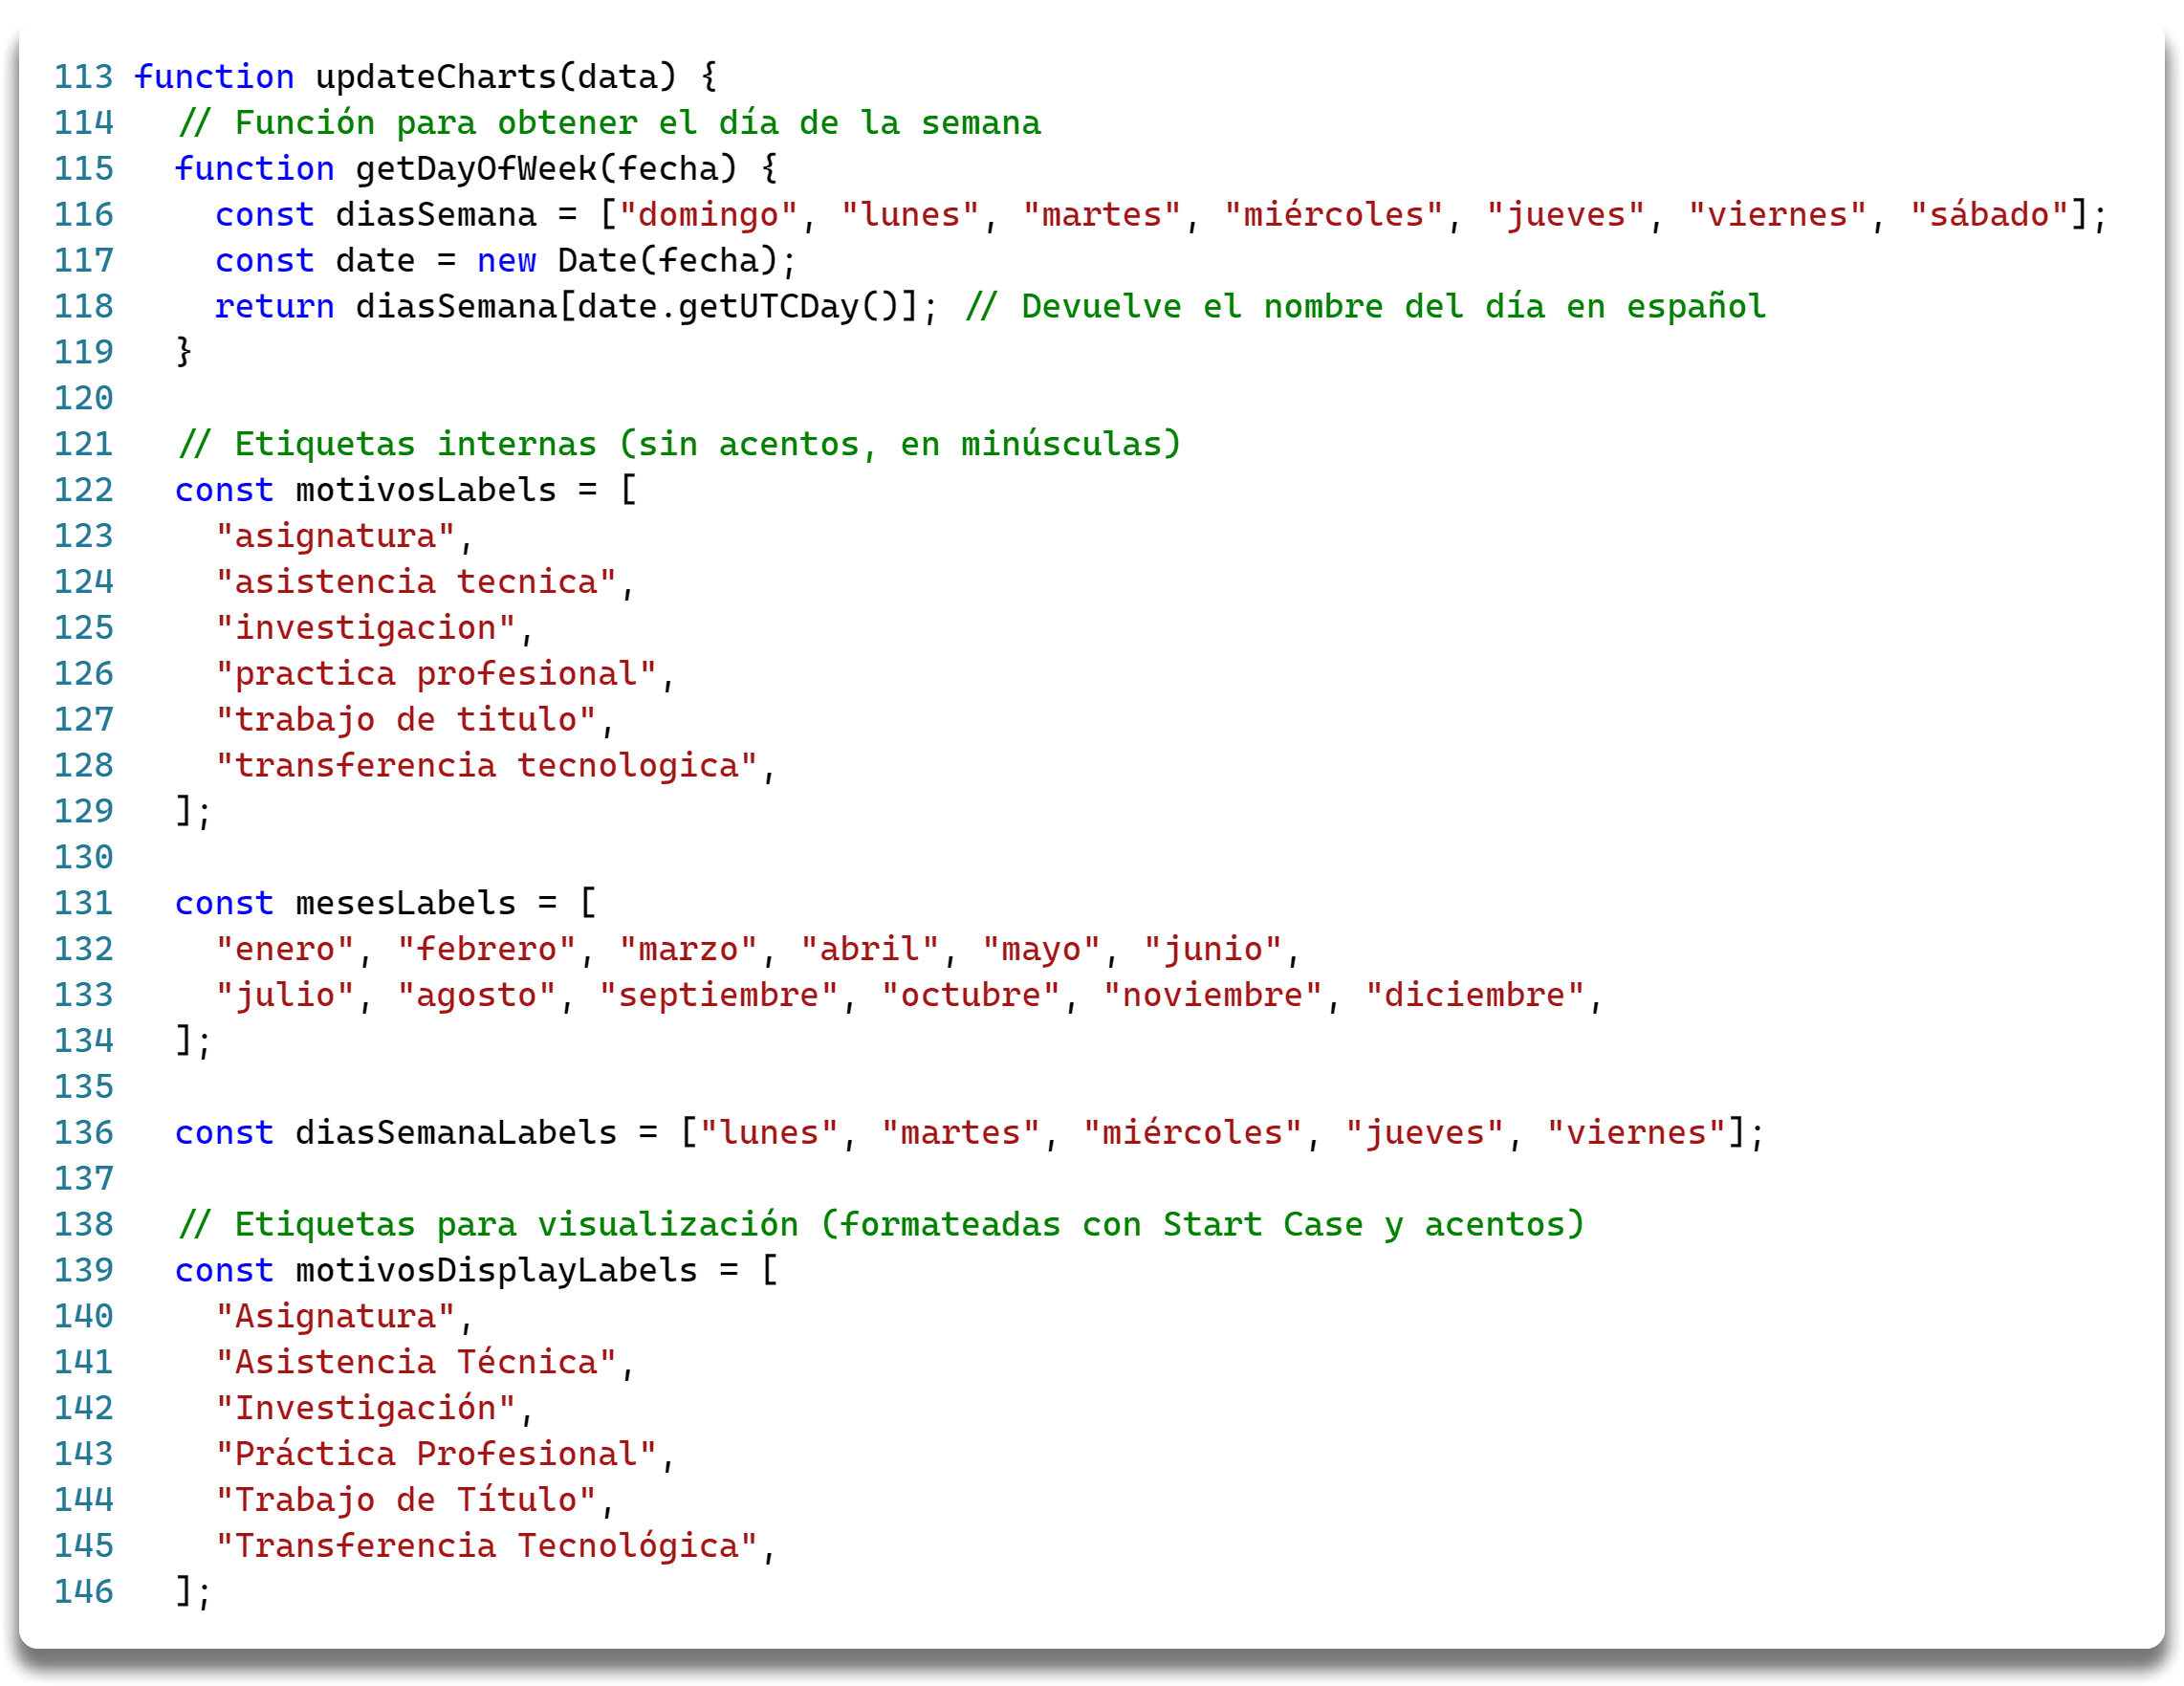
\includegraphics[width=\textwidth]{img/dataJS4.png}
				\caption{Archivo data.js Parte IV}
				\label{fig:dataJS4}
			\end{figure}
			\newpage
			\item Función que se encarga de actualizar las gr\'aficas, procesando los datos y insertandolos en las gr\'aficas:
			\begin{figure}[H]
				\centering
				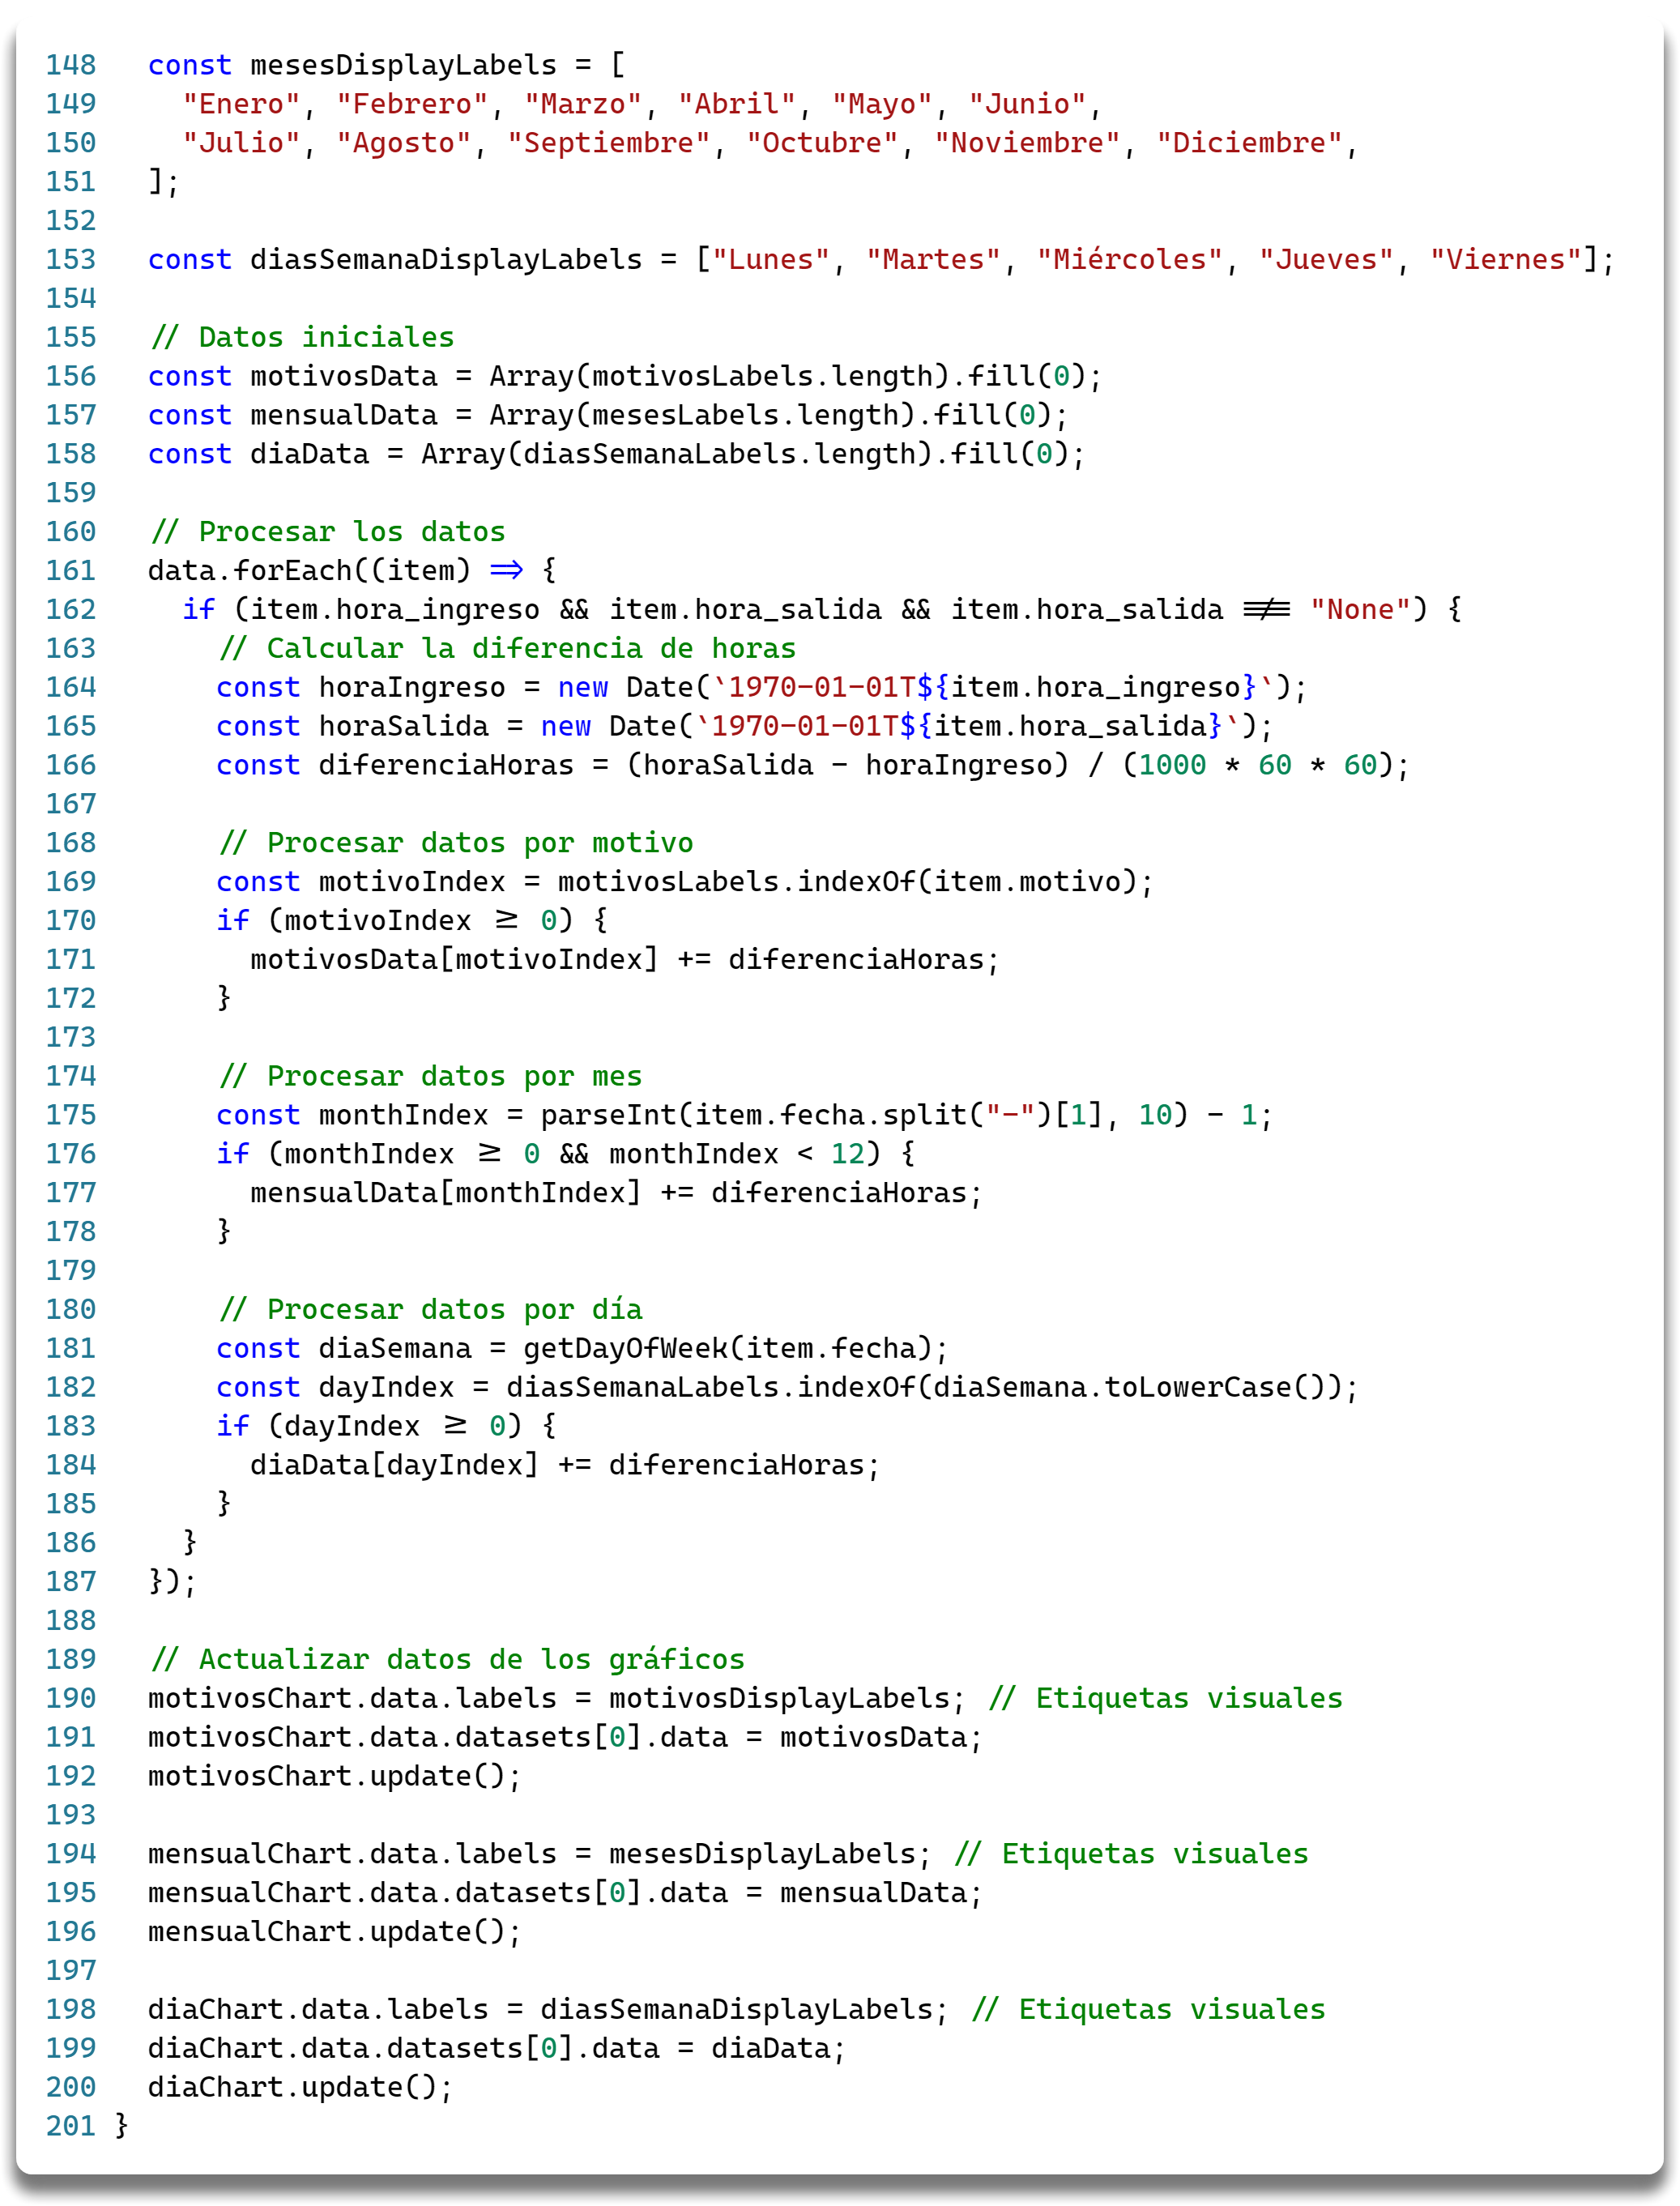
\includegraphics[width=\textwidth]{img/dataJS5.png}
				\caption{Archivo data.js Parte V}
				\label{fig:dataJS5}
			\end{figure}
			\newpage
			\item Función para resetear los valores de los filtros:
			\begin{figure}[H]
				\centering
				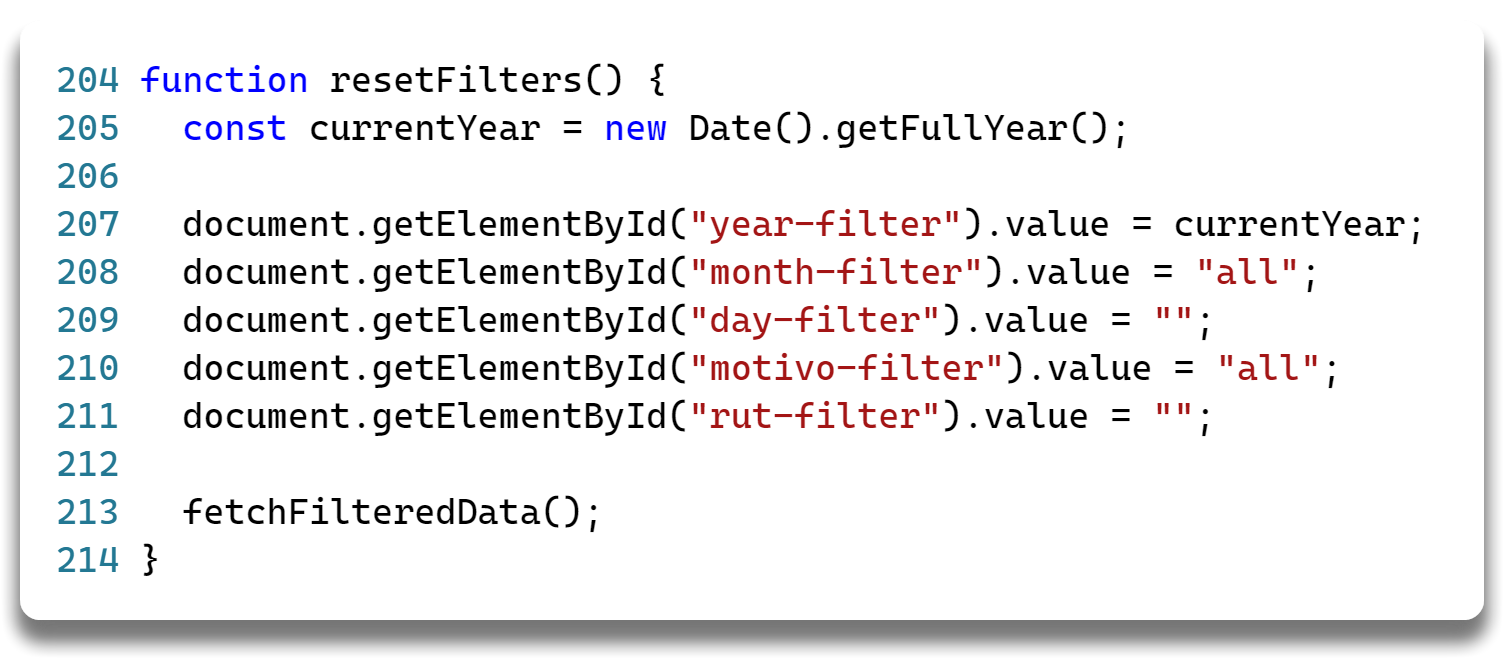
\includegraphics[width=\textwidth]{img/dataJS6.png}
				\caption{Archivo data.js Parte VI}
				\label{fig:dataJS6}
			\end{figure}
			\item C\'odigo que verifica que solo los rut con href puedan tener una referencia:
			\begin{figure}[H]
				\centering
				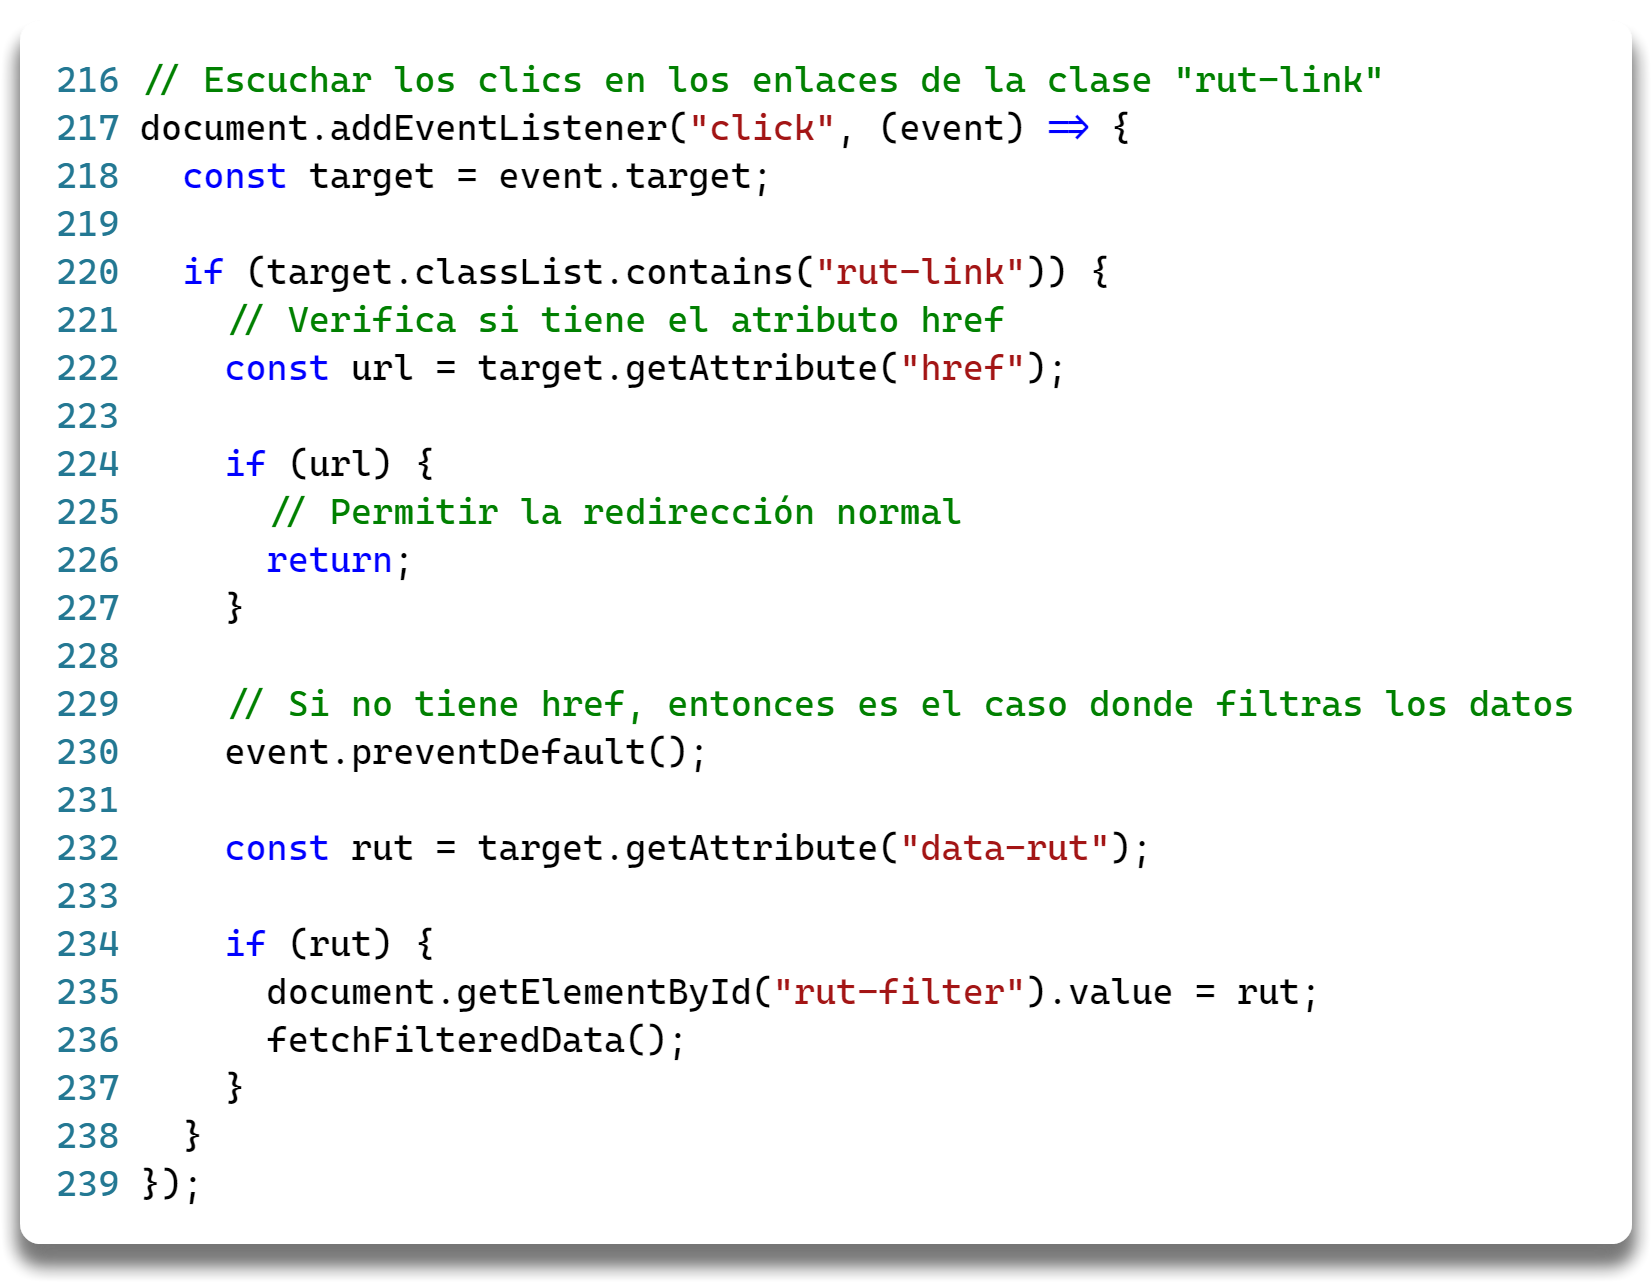
\includegraphics[width=\textwidth]{img/dataJS7.png}
				\caption{Archivo data.js Parte VII}
				\label{fig:dataJS7}
			\end{figure}
			\newpage
			\item Se vinculan los filtros a la función para que cada vez que ocurra algun cambio dentro de sus valores se active la función:
			\begin{figure}[H]
				\centering
				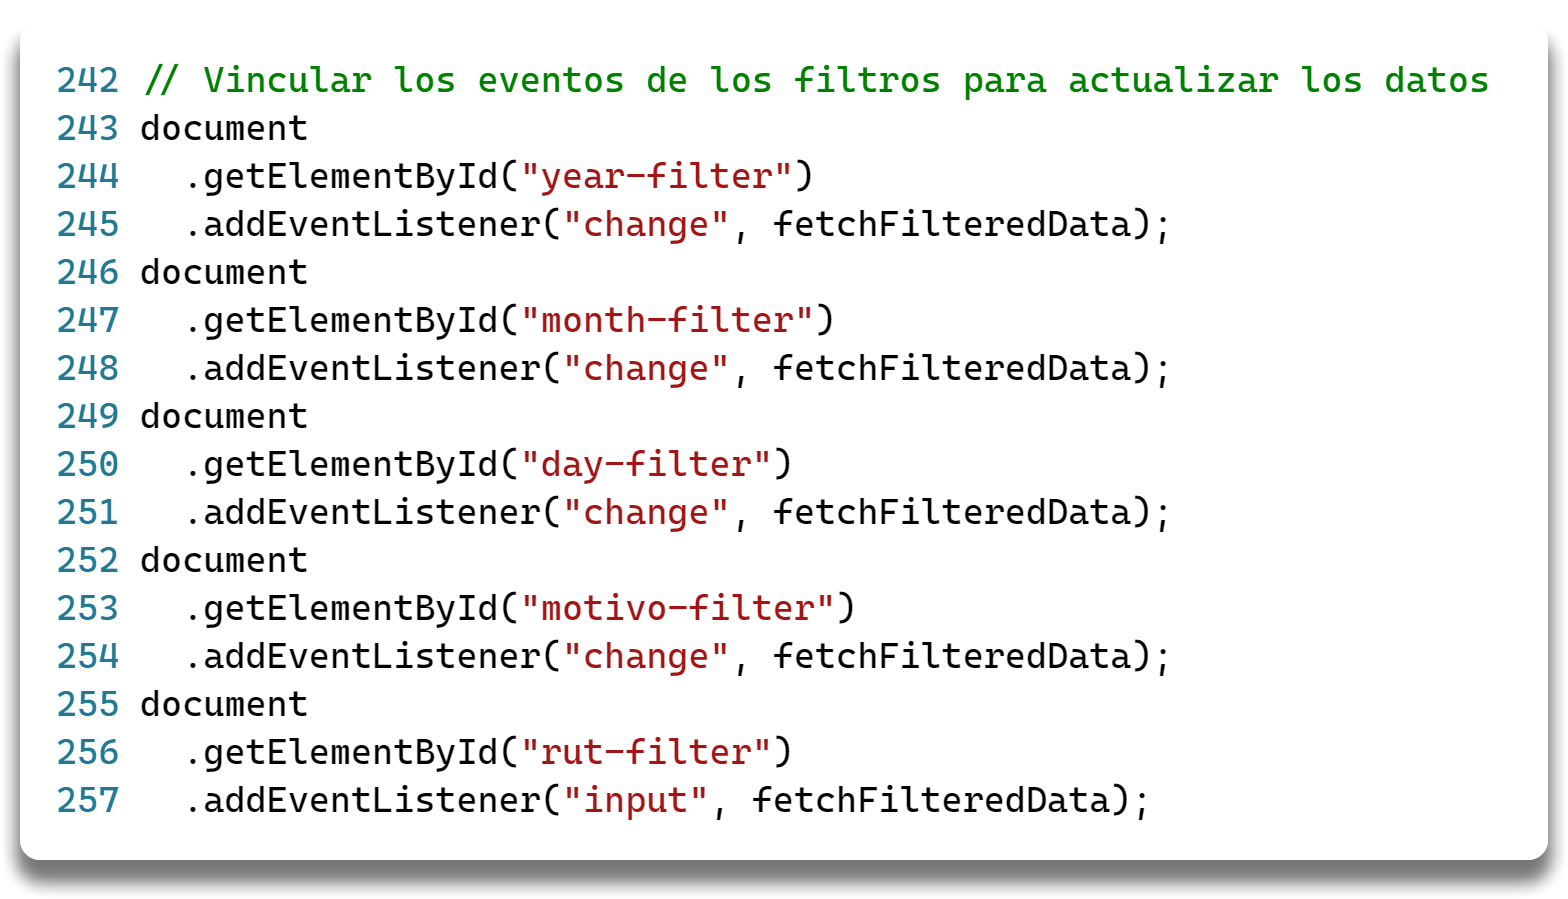
\includegraphics[width=\textwidth]{img/dataJS8.png}
				\caption{Archivo data.js Parte VIII}
				\label{fig:dataJS8}
			\end{figure}
			\item Cargamos los datos:
			\begin{figure}[H]
				\centering
				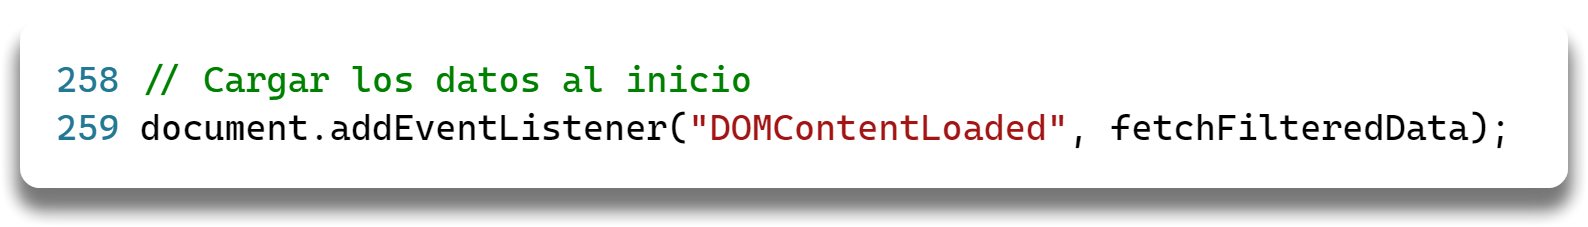
\includegraphics[width=\textwidth]{img/dataJS9.png}
				\caption{Archivo data.js Parte IX}
				\label{fig:dataJS9}
			\end{figure}
		  \end{enumerate}

		  \item \textbf{pagination.js}:
		  \begin{enumerate}
			\item Se muestra la tabla con 5 filas de datos:
			\begin{figure}[H]
				\centering
				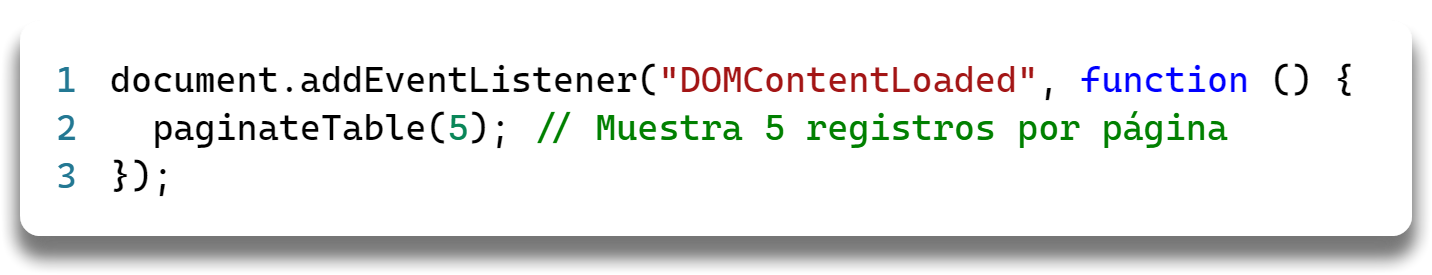
\includegraphics[width=\textwidth]{img/paginationJS1.png}
				\caption{Archivo pagination.js Parte I}
				\label{fig:paginationJS1}
			\end{figure}
			\newpage
			\item Función que renderiza inicialmente la tabla calculando la cantidad de filas a mostrar:
			\begin{figure}[H]
				\centering
				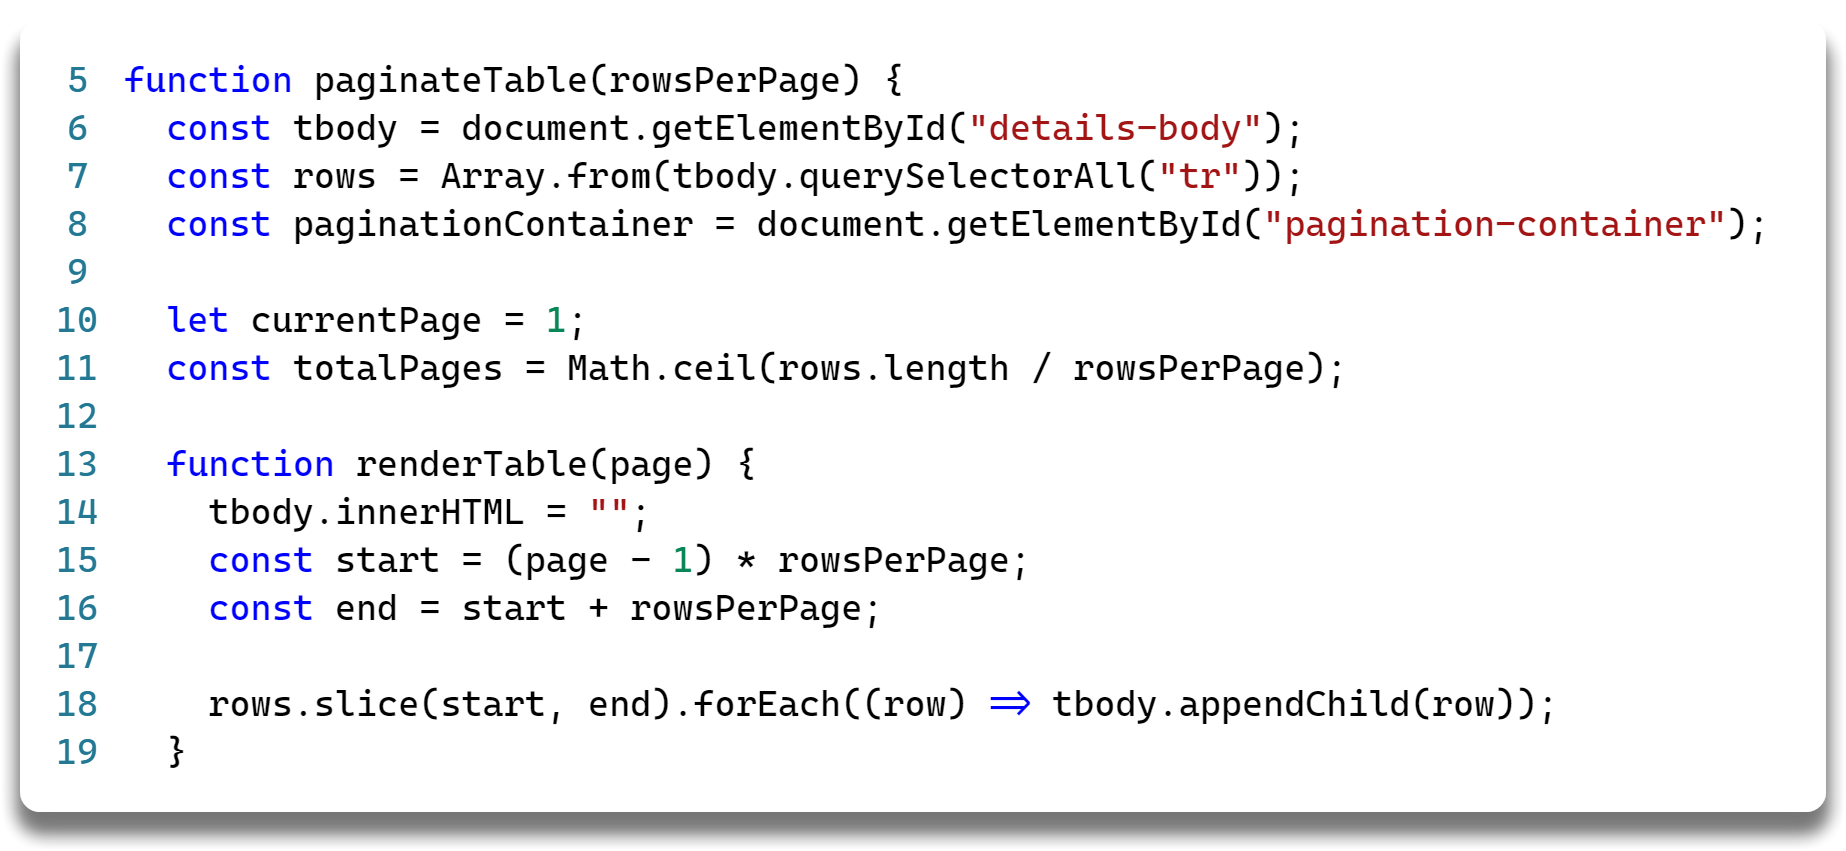
\includegraphics[width=\textwidth]{img/paginationJS2.png}
				\caption{Archivo pagination.js Parte II}
				\label{fig:paginationJS2}
			\end{figure}
			\item Función que renderiza los botones de la paginaci\'on, en este caso el bot\'on para Primera P\'agina:
			\begin{figure}[H]
				\centering
				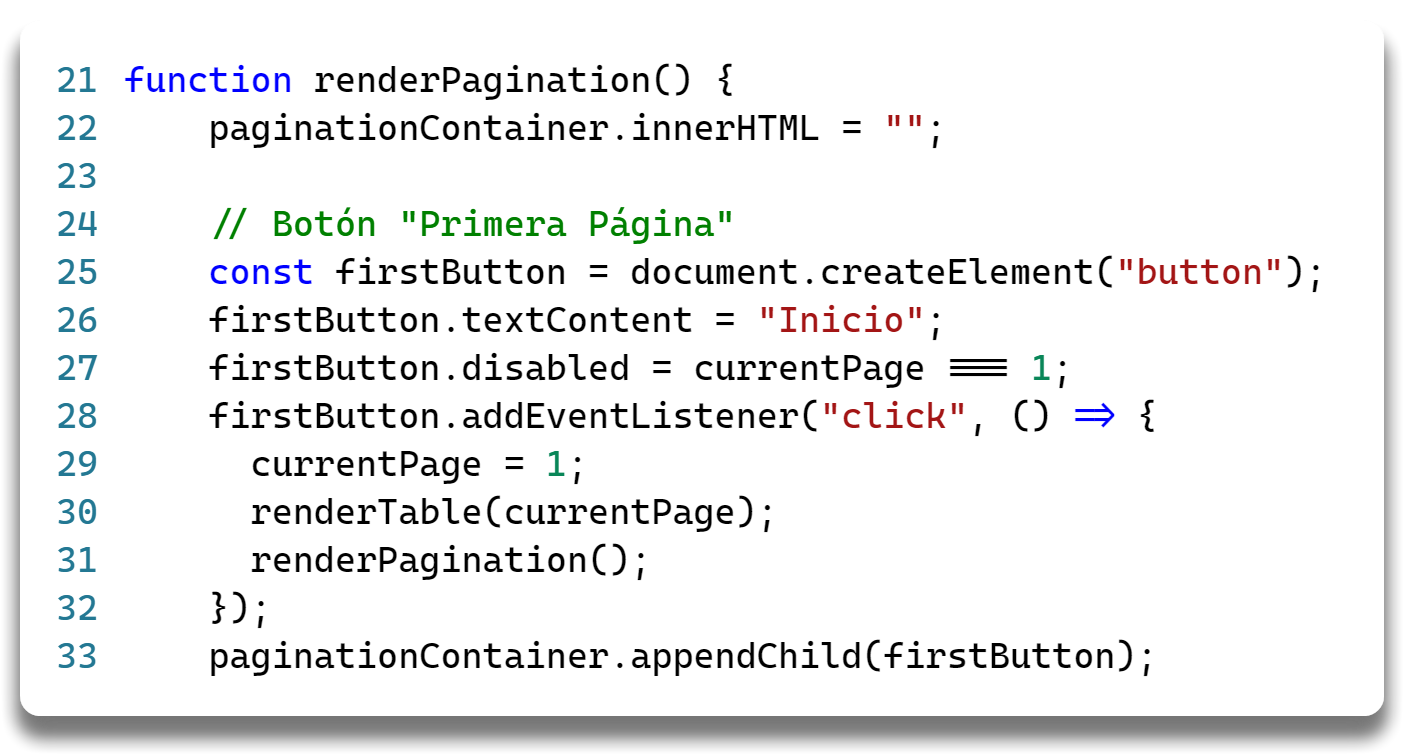
\includegraphics[width=\textwidth]{img/paginationJS3.png}
				\caption{Archivo pagination.js Parte III}
				\label{fig:paginationJS3}
			\end{figure}
			\newpage
			\item Se renderiza el bot\'on Anterior:
			\begin{figure}[H]
				\centering
				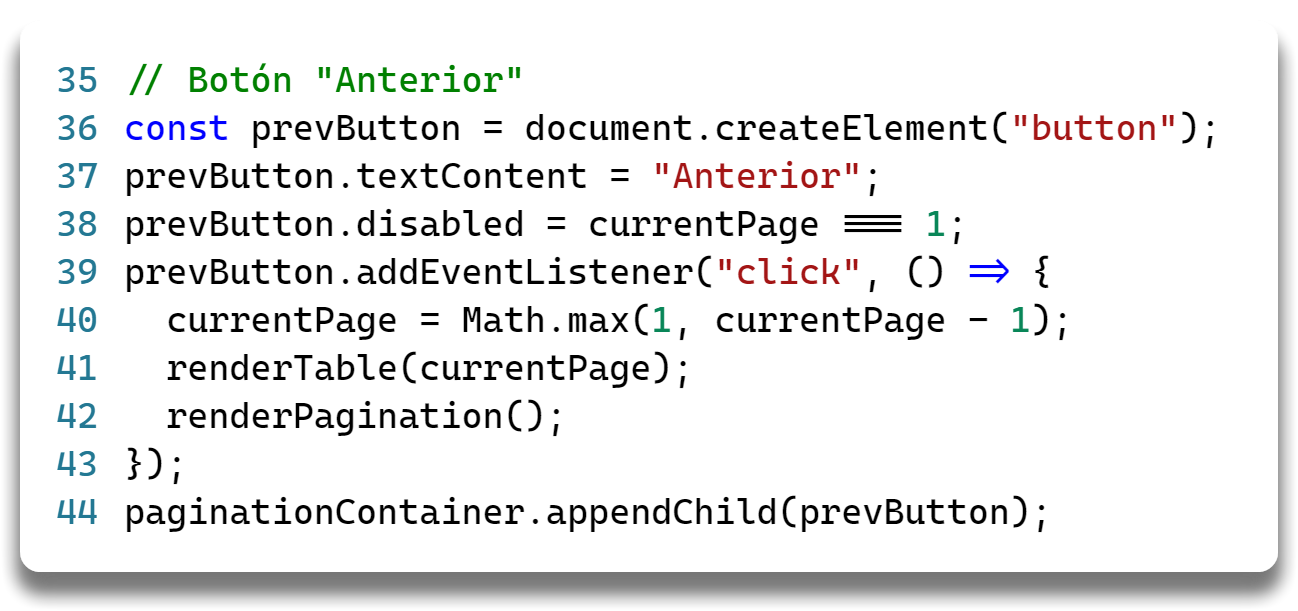
\includegraphics[width=\textwidth]{img/paginationJS4.png}
				\caption{Archivo pagination.js Parte IV}
				\label{fig:paginationJS4}
			\end{figure}
			\item Se renderiza el input para mostrar la paginaci\'on actual o elegir una:
			\begin{figure}[H]
				\centering
				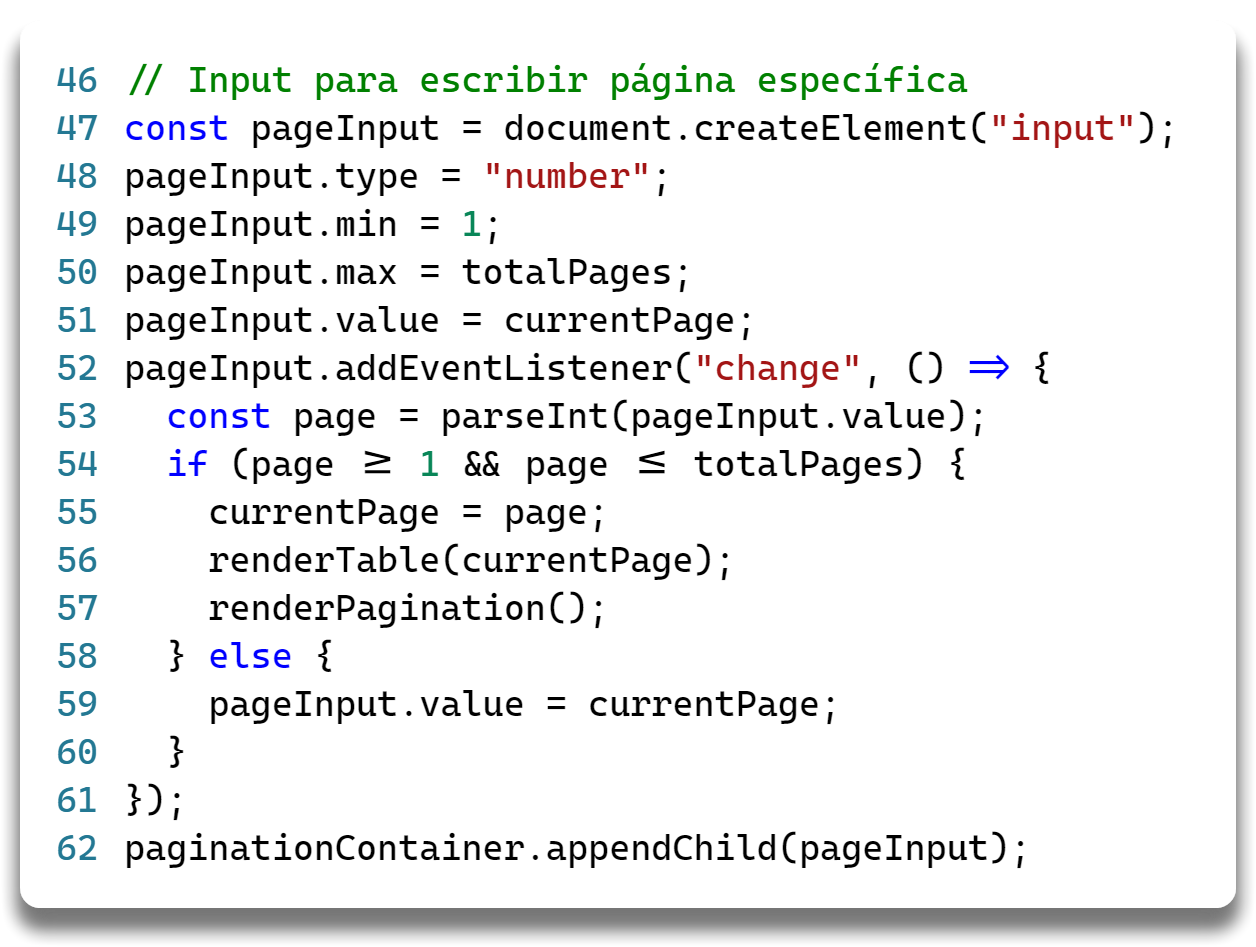
\includegraphics[width=\textwidth]{img/paginationJS5.png}
				\caption{Archivo pagination.js Parte V}
				\label{fig:paginationJS5}
			\end{figure}
			\item Se renderiza el boto\'on Siguiente:
			\begin{figure}[H]
				\centering
				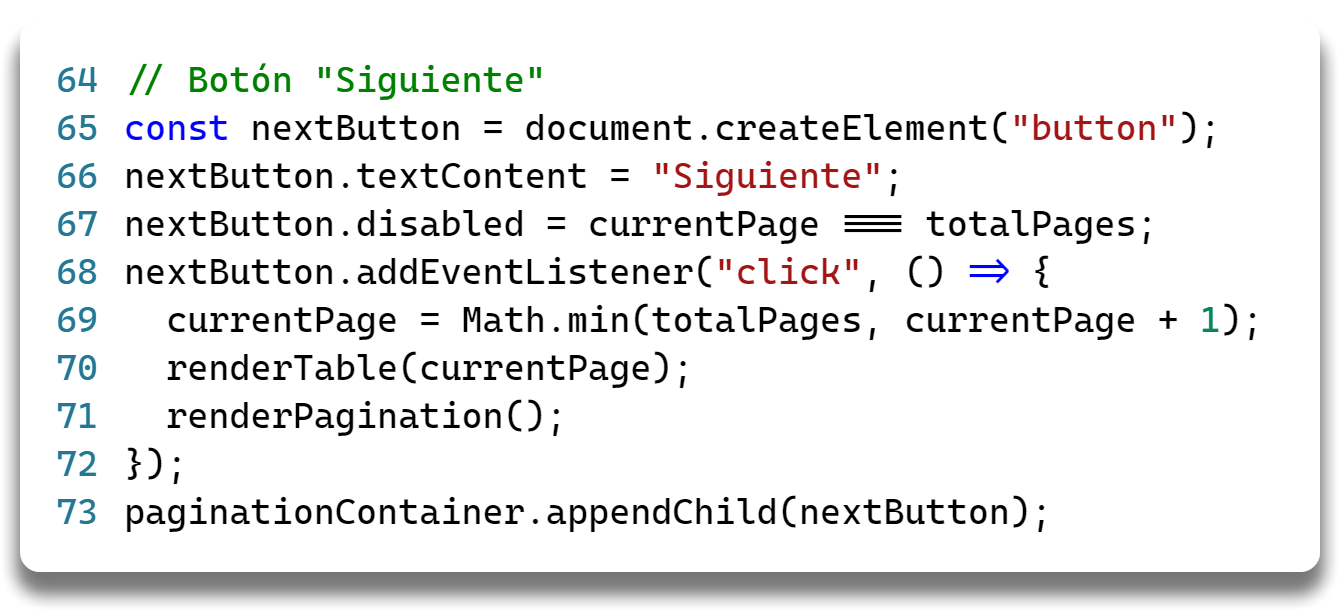
\includegraphics[width=\textwidth]{img/paginationJS6.png}
				\caption{Archivo pagination.js Parte VI}
				\label{fig:paginationJS6}
			\end{figure}
			\item Se renderiza el bot\'on \'Ultima P\'agina:
			\begin{figure}[H]
				\centering
				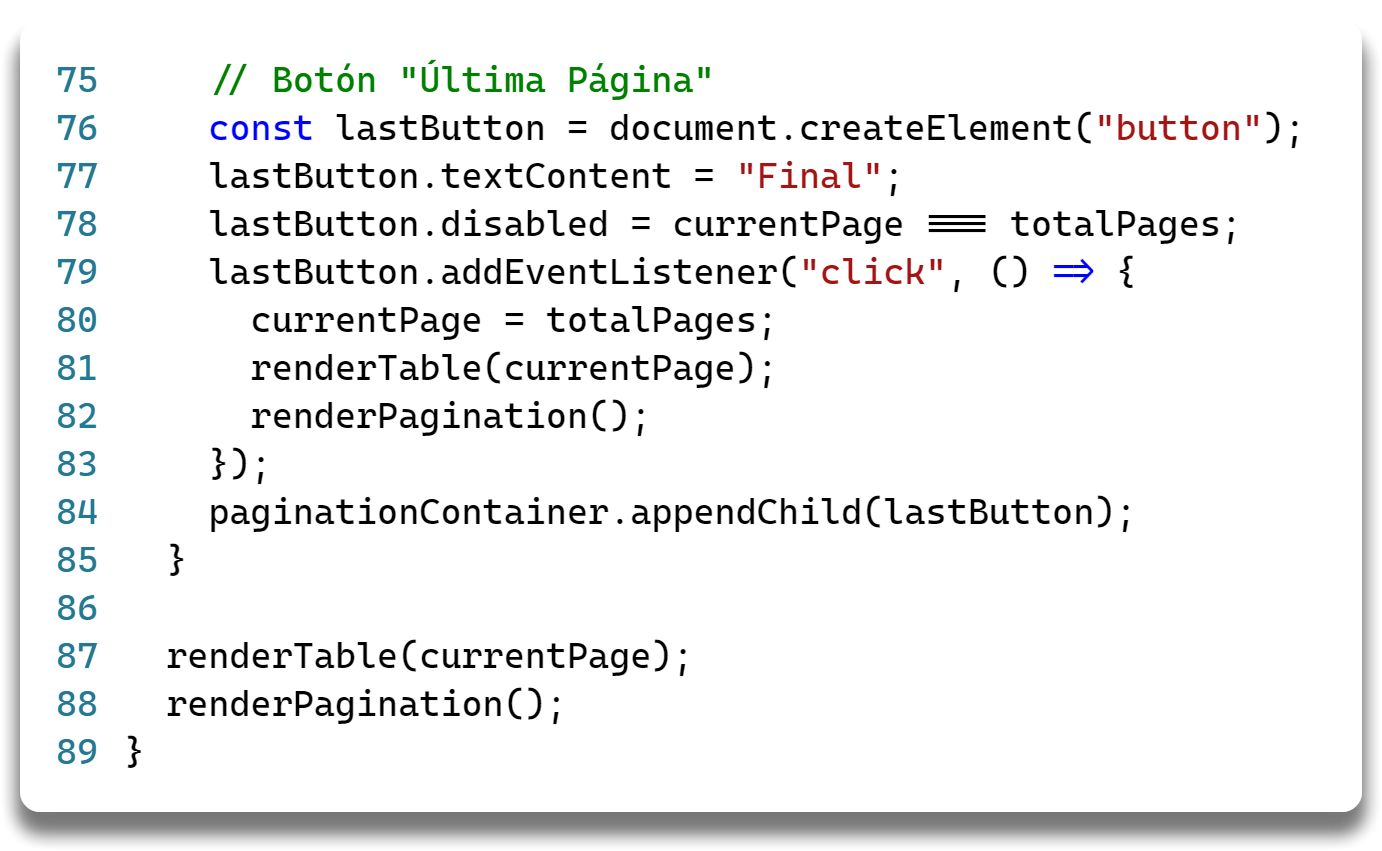
\includegraphics[width=\textwidth]{img/paginationJS7.png}
				\caption{Archivo pagination.js Parte VII}
				\label{fig:paginationJS7}
			\end{figure}
		  \end{enumerate}
		  \newpage
		  \item \textbf{sidebar.js}:
		  \begin{enumerate}
			\item Función para mostrar/esconder el SIDEBAR:
			\begin{figure}[H]
				\centering
				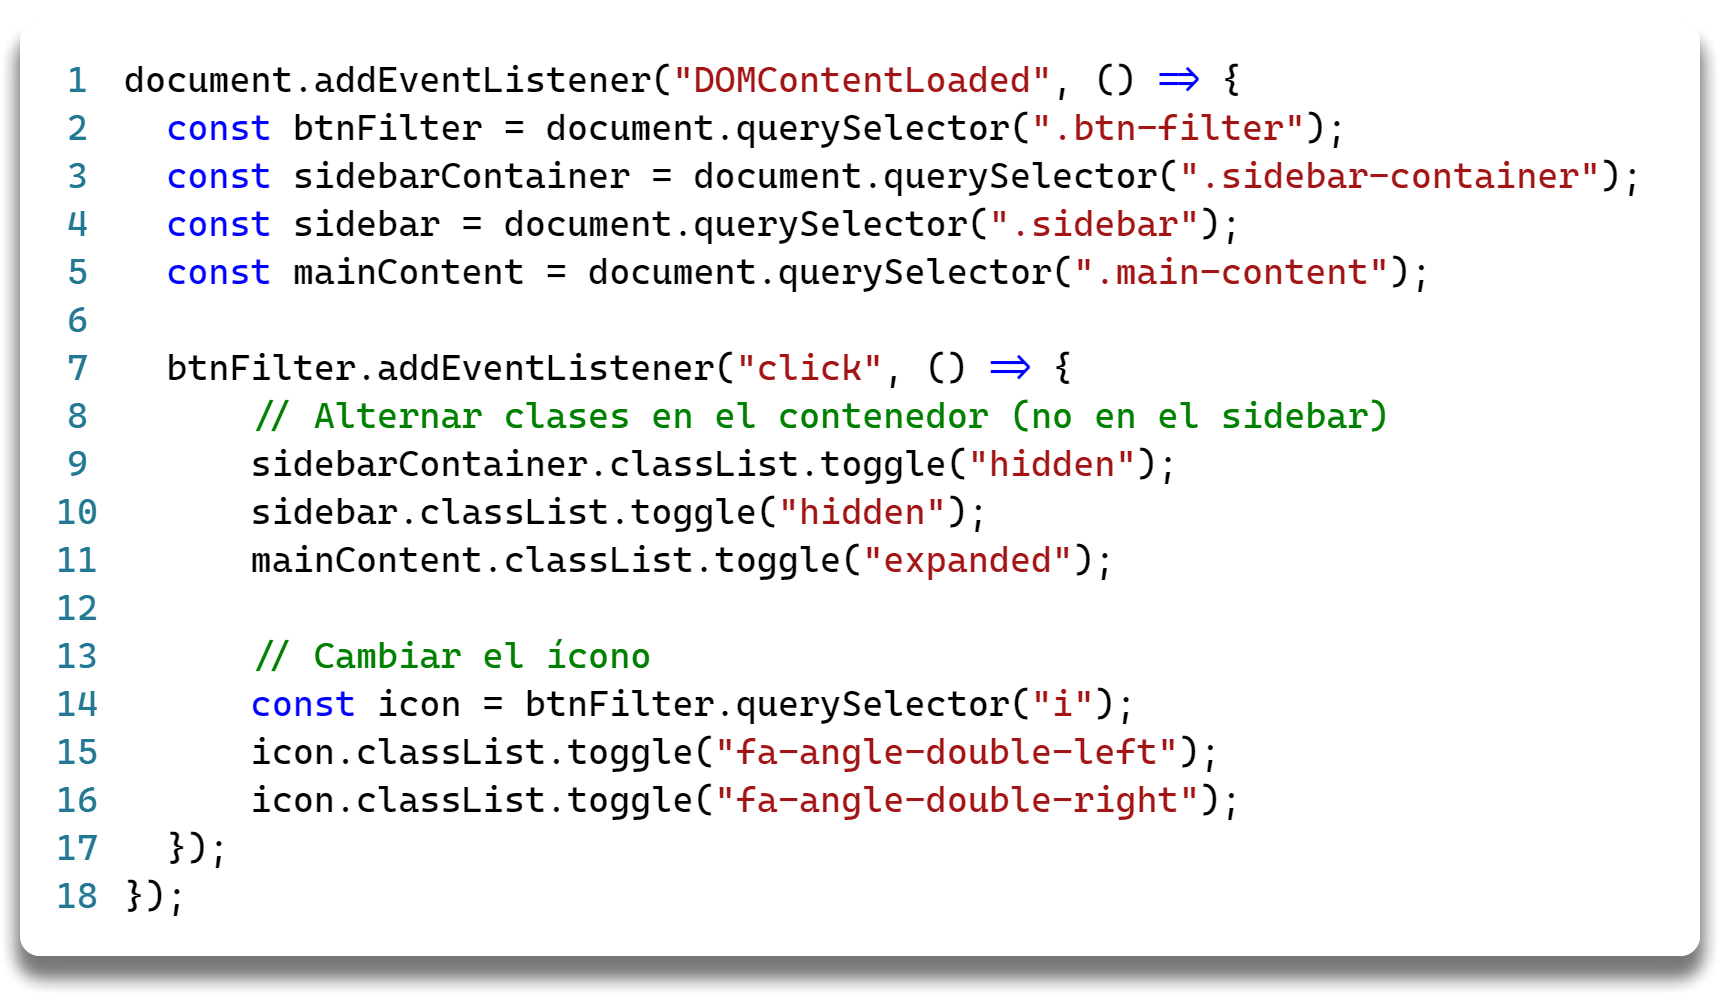
\includegraphics[width=\textwidth]{img/sidebarJS.png}
				\caption{Archivo sidebar.js}
				\label{fig:sidebarJS}
			\end{figure}
		  \end{enumerate}
\end{enumerate}
\subsection{Software registro de asistencia}
\subsubsection{Librerías}
\newpage
\section{Repositorio de GitHub}
\begin{figure}[H]
	\centering
	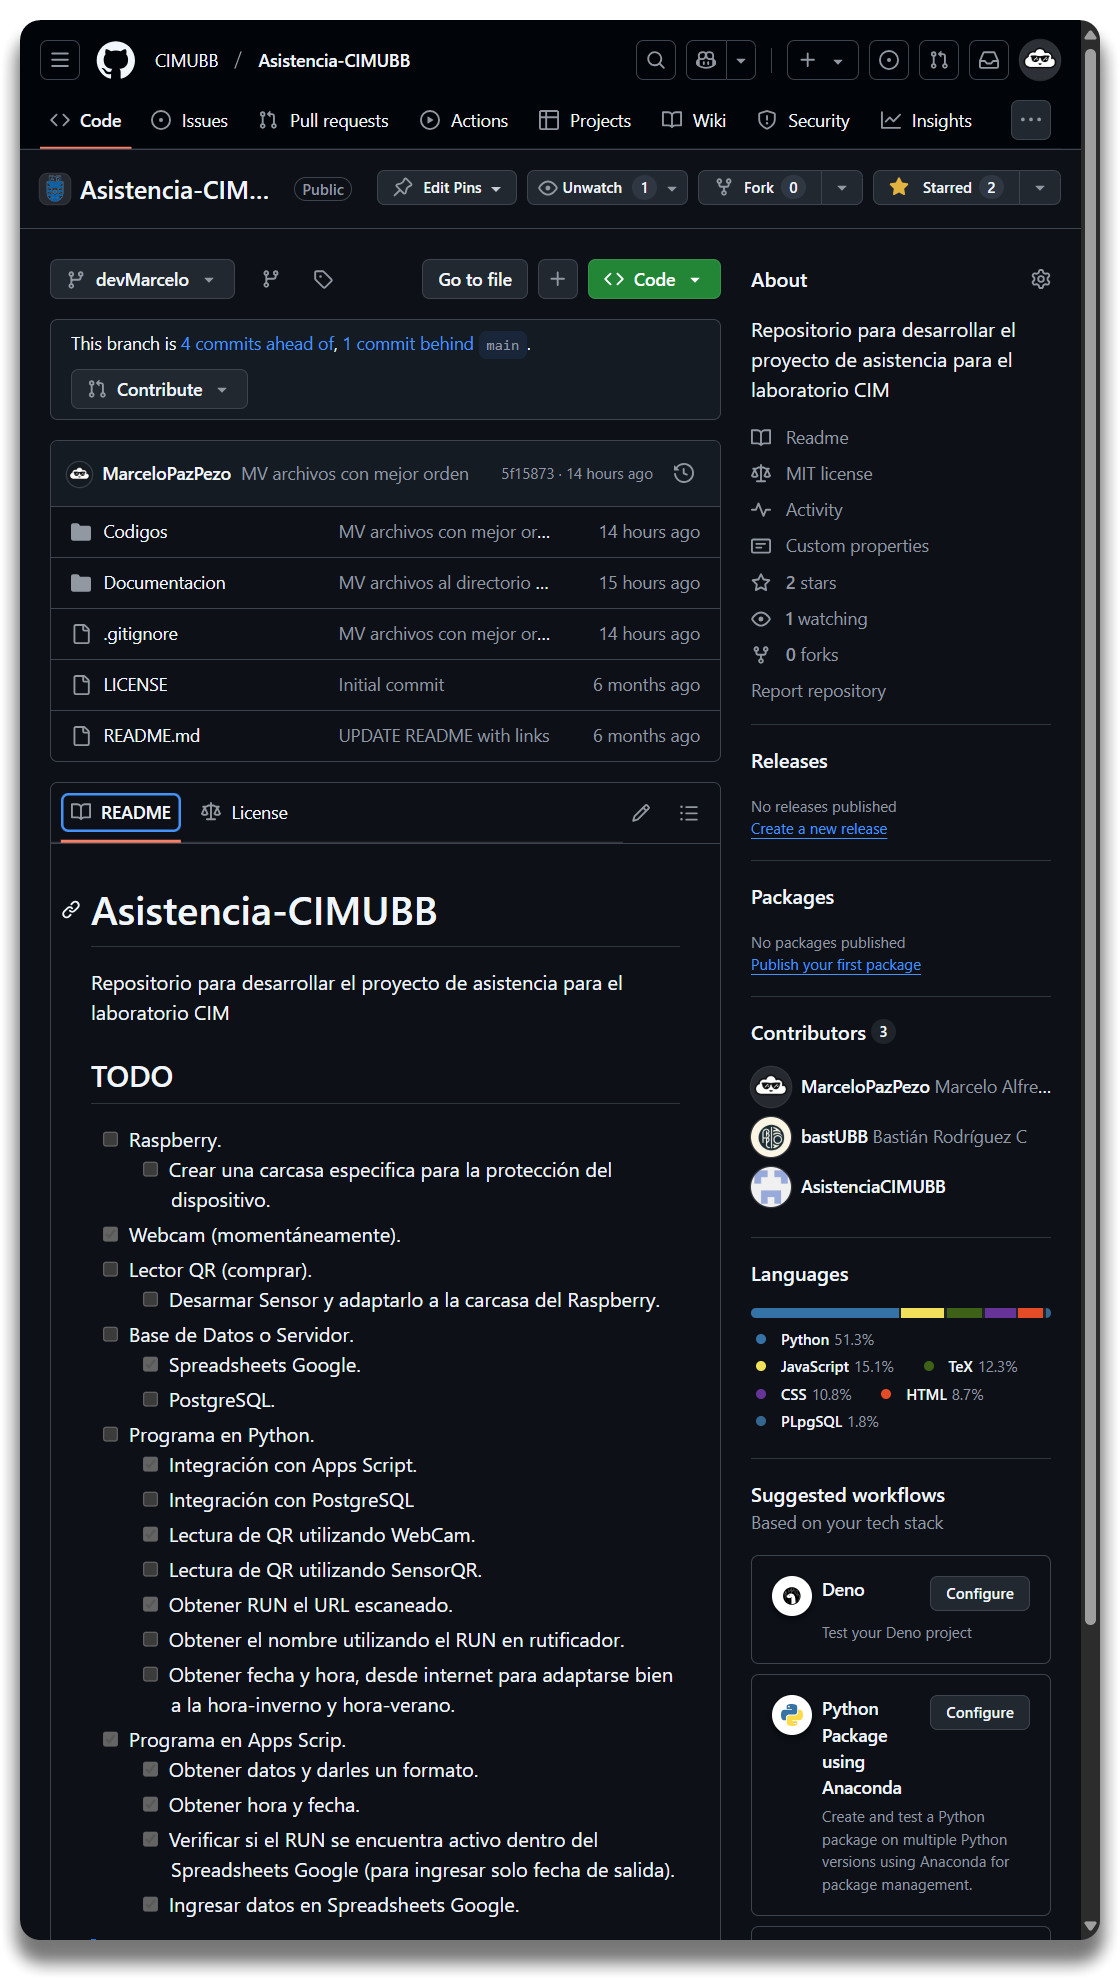
\includegraphics[scale=0.4]{img/capturaGitHub.png}
	\caption{Repositorio del proyecto \cite{githubRepositorio}}
	\label{fig:githubRepositorio}
\end{figure}
\newpage
\begin{thebibliography}{99}
	\bibitem{raspberryPi} Raspberry Pi 4 Model B 8 GB RAM \url{https://www.raspberrypi.com/products/raspberry-pi-4-model-b/}
	\bibitem{webcam} Logitech HD Webcam C270 \url{https://www.logitech.com/es-roam/products/webcams/c270-hd-webcam.960-000947.html?srsltid=AfmBOoqdKlo4lP1JIkMP6cvLw_Y6Kj5oKXIW-8gIEuyMUwLZRGhJMIwS}
	\bibitem{GM811} Documentación sensor QR GM811 \url{https://robu.in/wp-content/uploads/2024/08/GM811.pdf}
	\bibitem{randomString} Generate Random Strings and Numbers \url{https://www.browserling.com/tools/random-string}
	\bibitem{githubRepositorio} Asistencia-CIMUBB \url{https://github.com/CIMUBB/Asistencia-CIMUBB}
\end{thebibliography}
\end{document}